% svn info. These are modified by svn at checkout time.
% The last version of these macros found before the maketitle will be the one on the front page,
% so only the main file is tracked.
% Do not edit by hand!
\RCS$Revision: 1.43 $
%\RCS$HeadURL: svn+ssh://svn.cern.ch/reps/tdr2/notes/AN-11-higgs/trunk/AN-11-higgs.tex $
\RCS$Id: AN-11-higgs.tex,v 1.43 2011/09/19 20:49:23 psilva Exp $
%%%%%%%%%%%%% ptdr definitions %%%%%%%%%%%%%%%%%%%%%
\input{ptdr-definitions}

%extra-definitions
\newcolumntype{w}[1]{>{\raggedright\hspace{0pt}}p{#1}}
\providecommand{\ttbar}{{$t\bar{t}$}}
\providecommand{\Pythia}{{\textsc{Pythia}}\xspace}
\providecommand{\Tauola}{{\textsc{Tauola}}\xspace}
\providecommand{\Madgraph}{{\textsc{MadGraph}}\xspace}
\providecommand{\Alpgen}{{\textsc{Alpgen}}\xspace}
\providecommand{\Powheg}{{\textsc{Powheg}}\xspace}
\providecommand{\Sherpa}{{\textsc{Sherpa}}\xspace}
\providecommand{\MCatNLO}{{\textsc{MCatNLO}}\xspace}
\providecommand{\CMSSW}{{\textsc{CMSSW}}\xspace}
\providecommand{\pfMET}{{\textsc{pfMET}}\xspace}
\providecommand{\pflow}{{\textsc{pFlow}}\xspace}
\providecommand{\pfJET}{{\textsc{pfJET}}\xspace}
\providecommand{\Roofit}{{\textsc{Roofit}}\xspace}
\providecommand{\MET}{{$E_{T}^{miss}$}\xspace}
\providecommand{\centralMET}{{${\rm central}-E_{T}^{miss}$}\xspace}
\providecommand{\assocOvMET}{{${\rm assoc-}E_{T}^{miss} ({\rm other vtx})$}\xspace}
\providecommand{\assocMET}{{${\rm assoc-}E_{T}^{miss}$}\xspace}
\providecommand{\assocChMET}{{${\rm assoc-}E_{T}^{miss}({\rm charged})$}\xspace}
\providecommand{\cleanMET}{{${\rm clean-}E_{T}^{miss}$}\xspace}
\providecommand{\projMET}{{${\rm proj-}E_{T}^{miss}$}\xspace}
\providecommand{\RMET}{{${\rm red-}\vec{E}_{T}^{miss}$}\xspace}
\providecommand{\MC}{{\textsc{MC}}\xspace}
\providecommand{\PDF}{$\mathcal{P}_{df}$\xspace}

\linenumbers

%%%%%%%%%%%%%%%  Title page %%%%%%%%%%%%%%%%%%%%%%%%
\cmsNoteHeader{AN-11-higgs} % This is over-written in the CMS environment: useful as preprint no. for export versions
\title{Contribution to the search for the Higgs boson\\ in the ZZ$\rightarrow$ 2l2$\nu$ final state\\ with $\sqrt{s}=$7~TeV data}

%Author is always "The CMS Collaboration" for PAS and papers, so author, etc, below will be ignored in those cases

\address[cern]{CERN, Geneva, Switzerland}
%\author[cern]{The CMS Collaboration}
\author[cern]{P.~Silva}
\author[cern]{G.~Cerminara}
\author[cern]{L.~Quertenmont}
\author[cern]{M.~Mannelli}
\author[cern]{M.~Mulders}


% please supply the date in yyyy/mm/dd format. Today has been
% redefined to do so, but it should be fixed as of the final release date.
% For papers and PAS, \today is taken as the date the head file (this one) was last modified according to svn: see the RCS Id string above.
\date{\today}

% Abstract processing:
% 1. **DO NOT use \include or \input** to include the abstract: our abstract extractor will not search through other files than this one.
% 2. **DO NOT use %** to comment out sections of the abstract: the extractor will still grab those lines (and they won't be comments any longer!).
% 3. **DO NOT use tex macros** in the abstract: External TeX parsers used on the abstract don't understand them.
\abstract{
We summarize our contribution to the search for the Higgs boson in the high mass range ($m_H>$200~GeV/c$^2$)
using the CMS detector and the proton-proton collision data acquired in the 2011 run at a center-of-mass energy of 7~TeV.
The decay channel $H\rightarrow VV\rightarrow 2l2\nu$ where V is a vector boson (W or Z) is considered in the dilepton mass range of 76 to 106 GeV/c$^2$.
A dedicated event selection is outlined with the main purposes of
reducing the instrumental background resulting from the mismeasurement of missing transverse energy and exploring the kinematics of the Higgs events. 
In our search no excess is observed in data with respect to the Standard Model predictions
as well as in the presence of a sequential fourth family of high mass fermions
or in the fermio-phobic Higgs decay scenario.
Limits are set for the production of the Higgs boson in each one of the referred contexts.
}

% Do not comment out the following hypersetup lines (metadata). They will disappear in NODRAFT mode and are needed by CDS.
% Also: make sure that the values of the metadata items are sensible. For APS submissions, they are automatically converted to APS keywords.
\hypersetup{%
pdfauthor={CMG group},%
pdftitle={Searching for the Higgs in the ZZ to 2 leptons + 2 neutrinos final state with sqrt{s}=7 TeV data},%
pdfsubject={CMS},%
pdfkeywords={CMS, physics, Higgs boson, missing transverse energy}}

\maketitle %maketitle comes after all the front information has been supplied

\begin{small}
\tableofcontents
\end{small}

\newpage

%
% INTRODUCTION
%
\section{Introduction}
\label{sec:introduction}

We summarize our contribution to the search for the Higgs boson in the high mass range ($m_H>$200~GeV/c$^2$)
using the CMS detector and the proton-proton collision data acquired in the 2011 run at a center-of-mass energy of 7~TeV.
The decay channel $H\rightarrow VV\rightarrow 2l2\nu$ where V is a vector boson (W or Z) is considered in the dilepton mass range of 76 to 106 GeV/c$^2$.
A dedicated event selection is outlined with the main purposes of
reducing the instrumental background resulting from the mismeasurement of missing transverse energy and exploring the kinematics of the Higgs events. 
In our search no excess is observed in data with respect to the Standard Model predictions
as well as in the presence of a sequential fourth family of high mass fermions
or in the fermio-phobic Higgs decay scenario.
Limits are set for the production of the Higgs boson in each one of the referred contexts.

Our manuscript is organized as follows: we start by describing the general strategy adopted
to pre-select events under the $Z$-mass peak in Sec.~\ref{sec:triggerevselection};
dedicated studies for the reconstruction and resilience of the \MET measurement against mismeasurement of the hadronic recoil
and the contamination from pileup are detailed in Sec.~\ref{sec:met};
using the pre-selected events and what we find to be the most robust \MET measurement 
we develop a dedicated event selection for the search for the Higgs boson in the $2\ell2\nu$ sample in Sec~\ref{sec:higgssearch}.
After presenting the results obtained from 2011 data 
we discuss the selection efficiencies, data-driven background determination methods and the systematic uncertainties associated to our search.
In the final section (Sec.~\ref{sec:excllimits}) we perform the statistical analysis of the results obtained and set limits on the production
of the Higgs boson from the observed properties of the $2\ell2\nu$ sample. The procedure can be furthermore adopted to set limits on the
resonant production of di-boson final states decaying in the $2\ell2\nu$ sample where the dilepton invariant mass is restricted to the $Z$ boson resonant peak.


%
% EVENT SELECTION
%
\clearpage
\section{Trigger and event selection}
\label{sec:triggerevselection}

This section summarizes the trigger and tecniques explored for the dilepton event selection in data.
The data and MC samples used are also described.

%%
%% SAMPLES
%%
\subsection{Samples}
\label{subsec:samples}

As detailed in the introduction, all processes which are expected to produce at least one prompt lepton
have to be considered as relevant concurrent processes with the Higgs dileptonic sample. 
Due to the expected hadronic activity resulting from radiation and from the proton remnants,
a second lepton may be mimicked by a mismeasured jet.
This is the case for W+jets production and QCD.
Even if the lepton fake rate is expected to be low, these two processes have large cross sections
when compared with the expected production cross section for the Higgs boson.
Z boson production is however the most important concurrent process
as it produces two prompt leptons in the mass window of interest for this study.
Top quark and di-boson (WW,WZ,ZZ) production are also relevant but with much smaller cross section.
In particular top quark and WW boson production contribute to the non-resonant component of the dilepton spectrum.

Table~\ref{tab:mcsamples} summarizes the simulation samples which are used for all standard model processes
and which may mimick the signal under study.Table~\ref{tab:mcsignalsamples} summarizes the simulation samples used
to model the Higgs signal. Both gluon-gluon and vector boson fusion processes are considered as well as ZZ and WW decays of the Higgs boson.
The global tag START42\_V13 has been used to process \MC with
version 4\_2\_4 of the CMS official software (CMSSW).

\begin{table}[htp]
\caption{List of the SM Monte Carlo samples used in the comparison with 7~TeV data.
For the different processes (signal and background) considered 
the expected cross sections and the corresponding total integrated luminosity are quoted.
S11-S4 is used as a shortname for Summer11-PU\_S4\_START42\_V11.}
\label{tab:mcsamples}
\begin{center}
\hspace*{-1.5cm}
\begin{tabular}{llll} \hline\hline
\multicolumn{4}{c}{\bf Background processes} \\
Process                      & Dataset                                                                & $\sigma\cdot BR\cdot k$ (pb) & $\int \mathcal{L}$~(fb$^{-1}$)\\\hline
W+jets                       & /WJetsToLNu\_TuneZ2\_7TeV-madgraph-tauola/S11-S4-v1                    & 31314                        & 2.1\\
$Z/\gamma^{*}\rightarrow ll$ & /DYJetsToLL\_TuneZ2\_M-50\_7TeV-madgraph-tauola/S11-S4-v1              & 3048                         & 10.8\\
\ttbar                       & /TTJets\_TuneZ2\_7TeV-madgraph-tauola/S11-S4-v1                        & 165                          & 19.3 \\
\multirow{6}{*}{Single top}  & /T\_TuneZ2\_tW-channel-DR\_7TeV-powheg-tauola/S11-S4-v1 ($t$)          & 7.87                         & 78 \\
                             & /Tbar\_TuneZ2\_tW-channel-DR\_7TeV-powheg-tauola/S11-S4-v1 ($\bar{t}$) & 7.87                         & 103 \\
                             & /T\_TuneZ2\_t-channel\_7TeV-powheg-tauola/S11-S4-v1 ($t$)              & 41.92                        & 79 \\
                             & /Tbar\_TuneZ2\_t-channel\_7TeV-powheg-tauola/S11-S4-v1 ($\bar{t}$)     & 22.6                         & 64 \\
                             & /T\_TuneZ2\_s-channel\_7TeV-powheg-tauola/S11-S4-v1 ($t$)              & 3.19                         & 81 \\
                             & /Tbar\_TuneZ2\_s-channel\_7TeV-powheg-tauola/S11-S4-v1 ($\bar{t}$)     & 1.44                         & 26 \\
\multirow{3}{*}{Dibosons}    & /ZZ\_TuneZ2\_7TeV\_pythia6\_tauola/S11-v1                              & 5.9                          & 693 \\
                             & /WW\_TuneZ2\_7TeV\_pythia6\_tauola/S11-v1                              & 43                           & 98 \\
                             & /WZ\_TuneZ2\_7TeV\_pythia6\_tauola/S11-v1                              & 18.2                         & 234 \\\hline\hline
\end{tabular}
\end{center}
\end{table}

\begin{table}[htp]
\caption{List of the SM Monte Carlo samples used to model the Higgs signal.
The expected cross sections and branching ratios according to~\cite{LHCHiggsCrossSectionWorkingGroup:2011ti} are quoted in the table.
S11-S4 is used as a shortname for Summer11-PU\_S4\_START42\_V11;
ggHZZ, ggHWW, qqHZZ, qqHWW are used as shortnames for
GluGluToHToZZTo2L2Nu, GluGluToHToWWTo2L2Nu, VBF\_ToHToZZTo2L2NU, VBF\_HToWWTo2L2Nu correspondingly;
7TeV is used as shortname for 7TeV-powheg-pythia6.}
\label{tab:mcsignalsamples}
\begin{center}
\hspace*{-1cm}
\begin{tabular}{lllll} \hline\hline
\multicolumn{4}{c}{\bf Background processes} \\
Higgs mass (GeV/c$^2$)       & Dataset                        & $\sigma$ (pb)            & $BR(H\rightarrow VV)$ & $BR(VV\rightarrow 2l2\nu)$\\\hline
\multirow{4}{*}{200}         & /ggHZZ\_M-200\_7TeV/S11-S4-v1  & \multirow{2}{*}{5.27}    & 0.256                 & 0.0404 \\
                             & /ggHWW\_M-200\_7TeV/S11-S4-v1  &                          & 0.741                 & 0.0467 \\
                             & /qqHZZ\_M-200\_7TeV/S11-S4-v1  & \multirow{2}{*}{0.6371}  & 0.256                 & 0.0404 \\
                             & /qqHWW\_M-200\_7TeV/S11-S4-v1  &                          & 0.741                 & 0.0467 \\\hline
\multirow{4}{*}{300}         & /ggHZZ\_M-300\_7TeV/S11-S4-v1  & \multirow{2}{*}{2.422}   & 0.307                 & 0.0404 \\
                             & /ggHWW\_M-300\_7TeV/S11-S4-v1  &                          & 0.692                 & 0.0467 \\
                             & /qqHZZ\_M-300\_7TeV/S11-S4-v1  & \multirow{2}{*}{0.298}   & 0.307                 & 0.0404 \\
                             & /qqHWW\_M-300\_7TeV/S11-S4-v1  &                          & 0.692                 & 0.0467 \\\hline
\multirow{4}{*}{400}         & /ggHZZ\_M-400\_7TeV/S11-S4-v1  & \multirow{2}{*}{2.03}    & 0.269                 & 0.0404 \\
                             & /ggHWW\_M-400\_7TeV/S11-S4-v1  &                          & 0.582                 & 0.0467 \\
                             & /qqHZZ\_M-400\_7TeV/S11-S4-v1  & \multirow{2}{*}{0.161}   & 0.269                 & 0.0404 \\
                             & /qqHWW\_M-400\_7TeV/S11-S4-v1  &                          & 0.582                 & 0.0467 \\\hline
\multirow{4}{*}{500}         & /ggHZZ\_M-500\_7TeV/S11-S4-v1  & \multirow{2}{*}{0.865}   & 0.261                 & 0.0404 \\
                             & /ggHWW\_M-500\_7TeV/S11-S4-v1  &                          & 0.0946                & 0.0467 \\
                             & /qqHZZ\_M-500\_7TeV/S11-S4-v1  & \multirow{2}{*}{0.6371}  & 0.261                 & 0.0404 \\
                             & /qqHWW\_M-500\_7TeV/S11-S4-v1  &                          & 0.0946                & 0.0467 \\\hline
\multirow{4}{*}{600}         & /ggHZZ\_M-600\_7TeV/S11-S4-v1  & \multirow{2}{*}{0.3267}  & 0.272                 & 0.0404 \\
                             & /ggHWW\_M-600\_7TeV/S11-S4-v1  &                          & 0.558                 & 0.0467 \\
                             & /qqHZZ\_M-600\_7TeV/S11-S4-v1  & \multirow{2}{*}{0.05771} & 0.272                 & 0.0404 \\
                             & /qqHWW\_M-600\_7TeV/S11-S4-v1  &                          & 0.558                 & 0.0467 \\\hline\hline                          
\end{tabular}
\end{center}
\end{table}


Table~\ref{tab:datasamples} summarizes the data samples which are used for this study.
The global tag GR\_R\_42\_V20 has been used to process data with
version 4\_2\_4 of the CMS official software (CMSSW).
Residual jet energy corrections are applied to data.

\begin{table}[htp]
\caption{List of the primary datasets analyzed.
PD is used as a shortname for the primary datasets used, i.e. DoubleElectron, DoubleMu, MuEG and SingleMu.
The integrated luminosity and the run range corresponding to different data are shown in the rightmost columns.}
\label{tab:datasamples}
\begin{center}
\begin{tabular}{lll} \hline\hline
\multicolumn{3}{c}{\bf Data samples} \\
Dataset                         & $\int \mathcal{L}$ (pb$^{-1}$)  & Run range \\\hline
/PD/Run2011A-May10ReReco-v1/AOD & 215.2                           & {\small 160431-163869} \\
/PD/Run2011A-PromptReco-v4/AOD  & 930.7                           & {\small 165088-167913} \\
/PD/Run2011A-05Aug2011-v1/AOD   & 410.6                           & {\small 170722-172619} \\
/PD/Run2011A-PromptReco-v6/AOD  & 450.6                           & {\small 172620-173244} \\\hline
{\bf Total}                     & 2007.1                          &  \\
\hline\hline
\end{tabular}
\end{center}
\end{table}

The next section summarize the strategy adopted for the trigger, pre-selection, reconstruction and event selection.

%%
%% TRIGGER RECONSTRUCTION EVENT SELECTION
%%
\subsection{Trigger, reconstruction and event selection}
\label{subsec:trigrec}

The main aspects of the event selection are summarized as follows:

\begin{description}

%%% TRIGGER
\item[Trigger] unprescaled double lepton triggers available are used.
Unprescaled single muon triggers are also considered in order to recover possible inefficiencies from the trigger system acceptance
for larger values of the pseudo-rapidity ($|\eta|>$2.1).
Whenever possible, trigger thresholds are chosen below the nominal cut used for the offline reconstruction of electrons and muons.
Table~\ref{tab:datatrigger} summarizes the triggers used in data and in the \MC sample.
In the data triggers are vetoed sequentially in order to remove overlaps between the primary datasets~\cite{CMS-TWIKI-PDWG}.

\begin{table}[htp]
\caption{Triggers used in data and simulated in the \MC.
In data the version of the trigger depends on the dataset period. The HLT prefix has been omitted for simplicity all in the trigger names.
cI*Iso* is used as a shortname for CaloId*\_CaloIso* and tkI*Iso* as a short name for TrkId*\_TrkIso* where *=VL,L,T,VT.}
\label{tab:datatrigger}
\begin{center}
\hspace*{-1cm}
\begin{tabular}{lllll} \hline\hline
Trigger                                            & \multicolumn{4}{c}{Primary dataset/dilepton channel} \\\hline
\multicolumn{5}{c}{\bf Data} \\\hline
                                                                   & DoubleElectron & DoubleMu & MuEG & SingleMu  \\
{\small Ele17\_cILIsoVL\_Ele8\_cILIsoVL}                           & yes            & veto     & veto & veto      \\
{\small Ele17\_cITIsoVL\_tkIVLIsoVL\_Ele8\_\_cITIsoVL\_tkIVLIsoVL} & yes & veto     & veto & veto      \\
{\small DoubleMu7, Mu13\_Mu8}                                      & -              & yes      & veto & veto      \\
{\small Mu17\_Ele8\_cIL, Mu8\_Ele17\_cIL}                          & -              & -        & yes & veto       \\
{\small Mu17\_Ele8\_cITIsoVL}                                      & -              & -        & yes & veto       \\
{\small Mu8\_Ele17\_cITIsoVL}                                      & -              & -        & yes & veto       \\
{\small IsoMu17,IsoMu24}                                           & -              & -        & -   & yes      \\\hline
\multicolumn{5}{c}{\bf \MC} \\\hline
                                                                   & $ee$ & $\mu\mu$ & $e\mu$ &  \\
{\small Ele17\_cILIsoVL\_Ele8\_cILIsoVL\_v2}                       & yes  & -        & -      & \\
{\small DoubleMu7}                                                 & -    & yes      & -      & \\
{\small IsoMu17\_v5}                                               & -    & yes      & yes    & \\
{\small Mu8\_Ele17\_cIL\_v2}                                       & -    & -        & yes    & \\
{\small Mu10\_Ele10\_cIL\_v3}                                      & -    & -        & yes    & \\
{\small Mu17\_Ele8\_cIL\_v2}                                       & -    & -        & yes    & \\\hline\hline
\end{tabular}
\end{center}
\end{table}

%%% PRE-SELECTION
\item[Pre-selection filters] are applied to minimize the contamination from beam-gas interactions, beam-halo and calorimeter noise.
Table~\ref{tab:preselflow} summarizes the number of events in data which are found passing each filter.
It can be seen that the beam halo filter mostly affects the muon sample, as expected, as it is based on the signals
left in the CSC's by halo muons.

\begin{table}[htp]
\caption{Events selected after each pre-selection step for the different datasets considered.
The last column summarizes the \% of the original primary dataset considered after applying all the event filters.}
\label{tab:preselflow}
\begin{center}
\begin{tabular}{lllllll} \hline\hline
\multirow{2}{*}{Sample} & \multicolumn{5}{c}{Events accepted (10$^7$)} \\
                        & in PD          &  no scrap  & $\geq$ 1 vertex & no HBHE noise & no beam halo & \% pre-filtered\\\hline
DoubleMu                & 3.365          & 3.365      & 3.298           & 3.296         & 3.260        & 96.9\% \\
SingleMu                & 7.380          & 7.380      & 7.374           & 7.372         & 7.314        & 99.1\% \\
DoubleElectron          & 4.272          & 4.272      & 4.272           & 4.271         & 4.263        & 99.7\% \\
MuEG                    & 2.829          & 2.829      & 2.829           & 2.828         & 2.823        & 99.8\% \\\hline\hline
\end{tabular}
\end{center}
\end{table}

%%% PRIMARY VERTICES
\item[Primary vertices] must be found within maximum range of 24~cm along the beam line (z) and within a 2~cm cylinder around the beam line ($\rho$)..
The minimum number of degrees of freedom (n.d.o.f.) of the vertex fit is required to be 4.
In case of multiple primary vertices the primary vertex is chosen has the one with highest flux of charged particles in the transverse plane,
i.e. the vertex with highest $\displaystyle{\sum_{tracks}} p_T^2$ flux.
Fig.~\ref{fig:vertexcontrol} shows two control distributions for the selected vertices in data and in the simulation:
the vertex multiplicity and the transverse momentum resulting from the sum of all the charged particle flow candidates which are associated to the primary vertex of the event.
Overall a fair agreement is found between data and \MC but it is visible that the procedure used to re-weight the pileup in the simulation
does not reproduce fully the real pileup scenario which evolved throughout different stages during the 2011 run data taking.
The sum of the charged particle flow candidates associated to the primary vertex is a quantity which is expected to be robust against pileup variations
and which shows sensitivity to processes in which undetectable particles are produced such as : $W$, top quark and di-boson production.
In both distributions the \MC does not include the low mass Drell-Yan contribution which contributes to an overall scale-factor of $\approx$ 10\%. 

\begin{figure}[htp]
\begin{center}
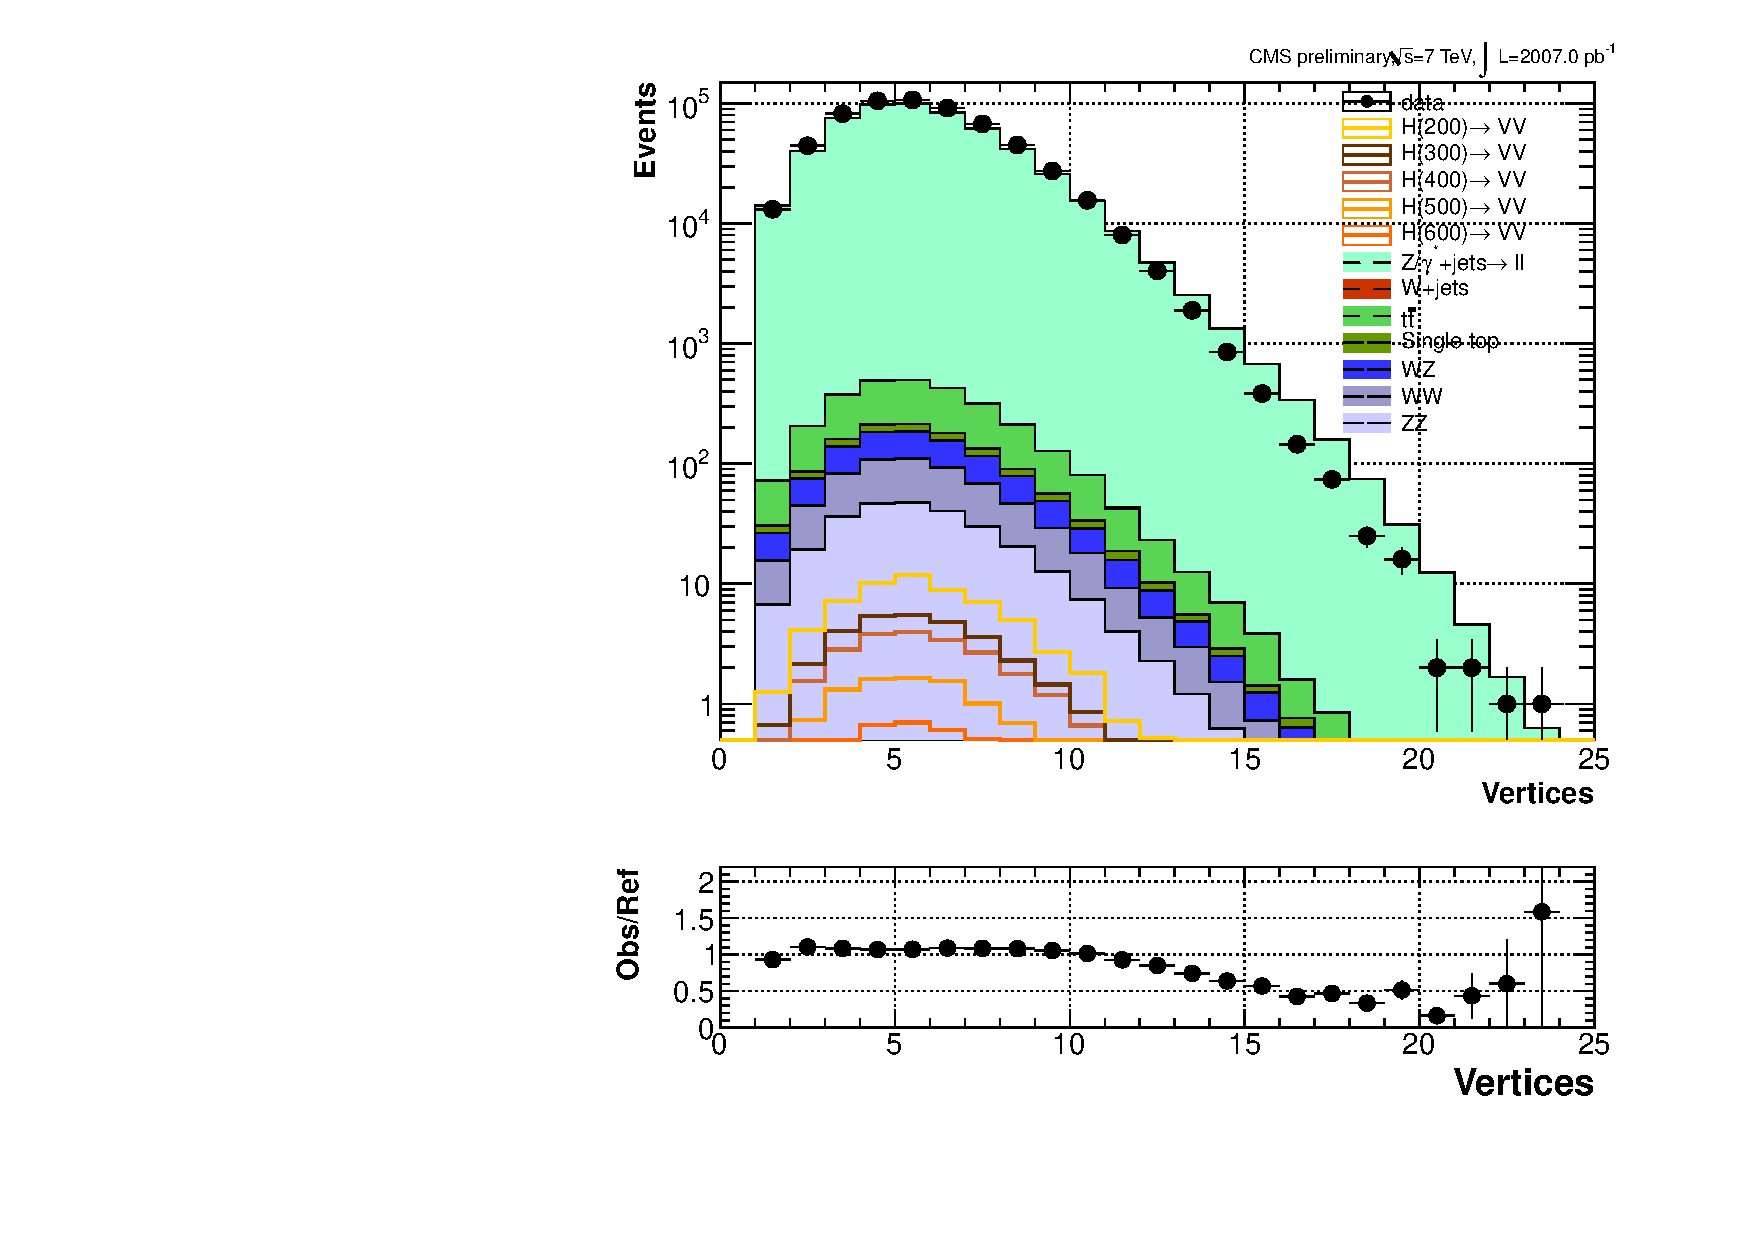
\includegraphics[width=0.4\textwidth]{img/mumu_ngoodvertex}
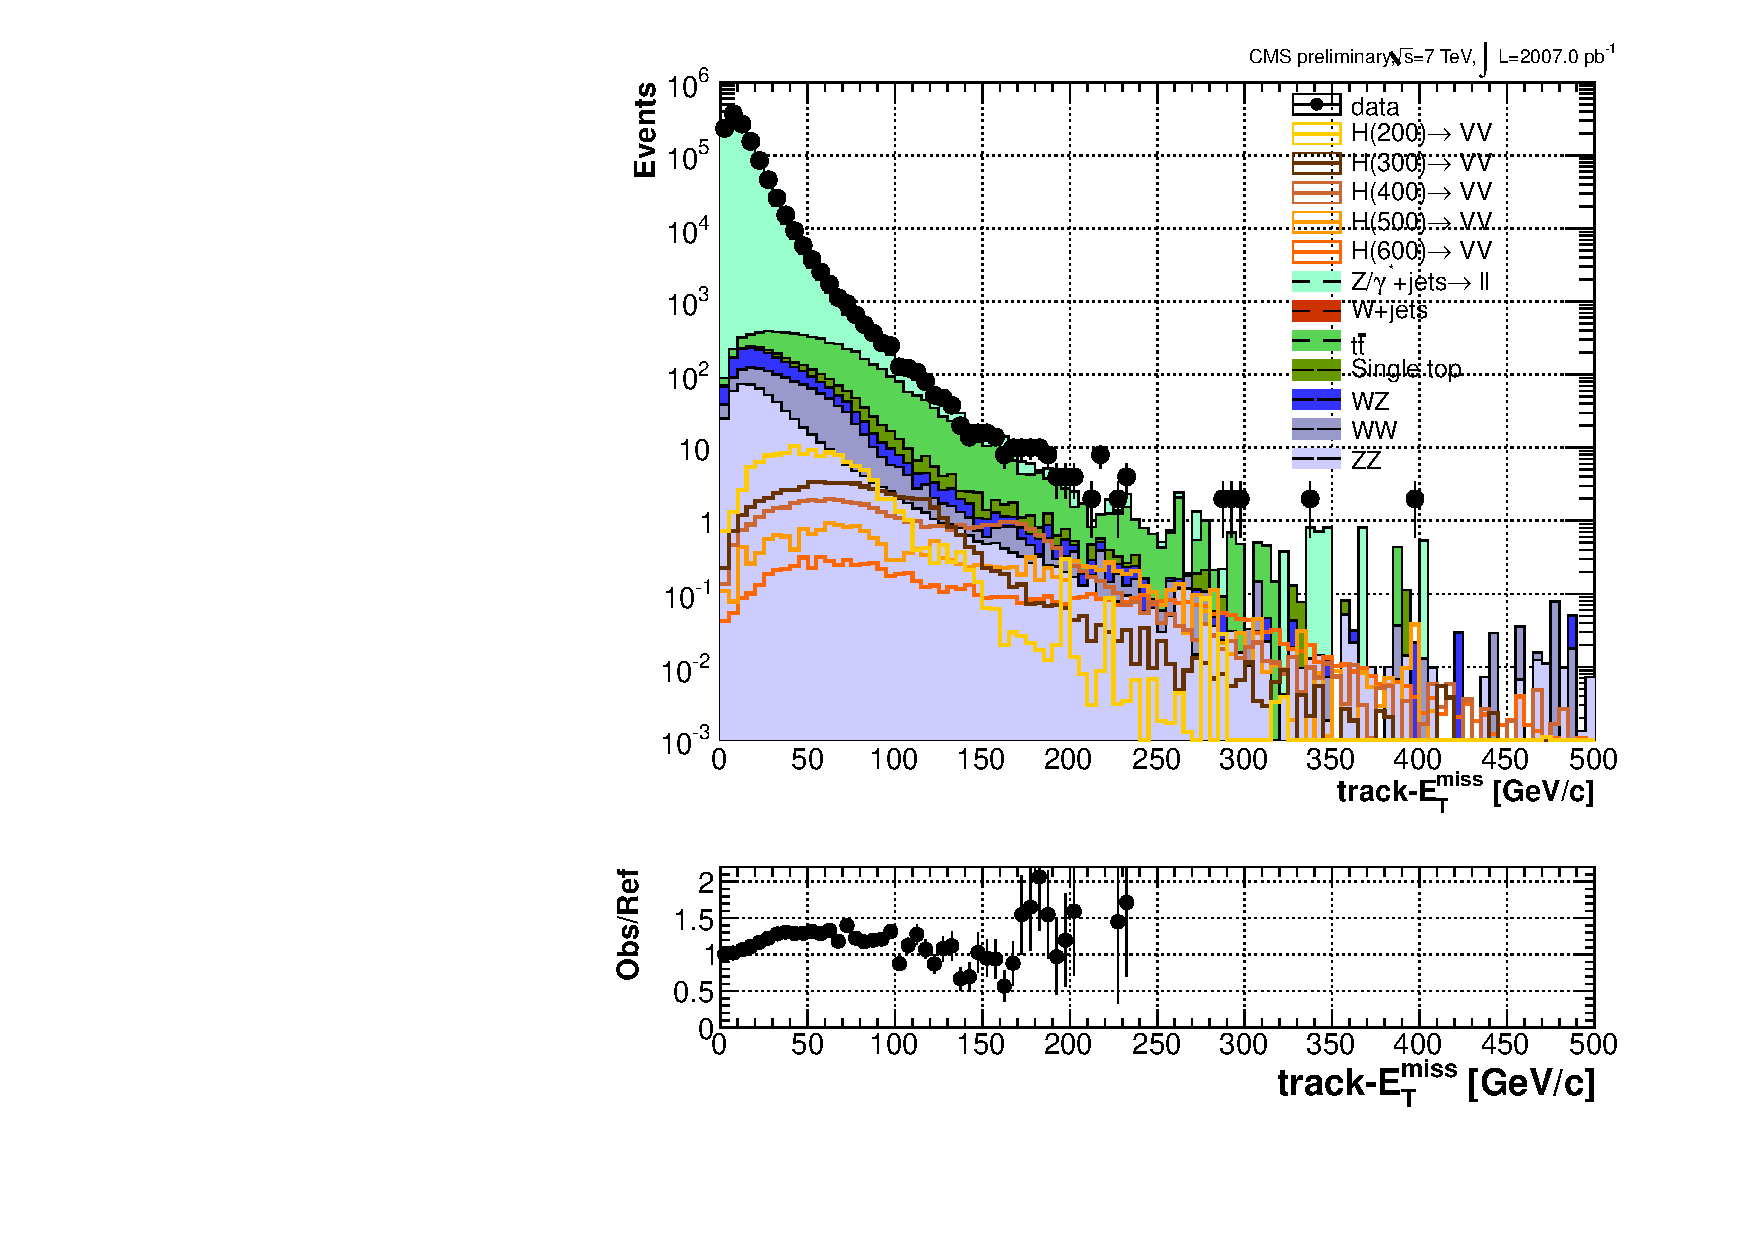
\includegraphics[width=0.4\textwidth]{img/mumu_trkmet}
\caption{Distribution of the vertex multiplicity ({\em left}) and the transverse momentum resulting from the sum of all charged particle-flow candidates associated to the primary vertex of the event ({\em right}).
The bottom plots show the ratio between the total \MC prediction and the observed data.}
\label{fig:vertexcontrol}
\end{center}
\end{figure}




%%% LEPTONS
\item[Leptons] leptons (electrons or muons) are required to be reconstructed with at least $p_T>$5~GeV/c and $|\eta|<$2.5 (2.4) for electrons (muons). 

Electrons can be seeded from either the electromagnetical calorimeter (ECAL driven) or the tracker (tracker driven).
Electrons reconstructed in the ECAL barrel to endcap transition are not considered for this study in order to reduce the contamination from fakes and to 
minimize the impact of mismeasurement of the lepton energies which translates to a mismeasurement of the missing transverse energy of the event.
The impact parameter of the electron track is required to be consistent with prompt production from the beam spot within $|d_0|<$0.04~cm.
Non-prompt electrons, from photon conversions in the tracker material, are vetoed by geometric requirements
applied on partner tracks (dist$<$0.02~cm and $\Delta\cot\theta<$0.02) and by requiring a maximum of 1 lost tracker hit. 
For each electron it is also required that no tracker or global muon with at least 10 tracker hits is found within a $\Delta R<$0.1 of the reconstructed electron.
Electron identification relies on a simple cut based identification algorithm 
which depends on the supercluster shape, its alignment with the track which is associated to electron and H/E.
The electron-id cuts are tuned specifically for each ECAL region (barrel and endcap) in order to yield 
an expected efficiency for the reconstruction of electrons from $W \rightarrow e\nu$ decays.
Details on the VBTF specific requirements can be found in~\cite{CMS-TWIKI-VBTF11}.
For this study we require at pre-selection that the VBTF-95 working point is verified. 
For electron candidates to be considered as a leg of the dilepton candidate the verification of the VBTF-85 working point is further required
as well as having $p_T>$20~GeV/c. 
The choice on these electron-ids is trigger oriented, as the trigger identification requirements consist in looser versions of the VBTF requirements.

Muon identification is mainly based on the $\chi^2$ fit of the global track and on the number of hits in the tracker and muon stations.
Loose muons are required to verify the TrackerMuonArbitrated criteria, i.e. to be tracker muons, 
and to be consistent with prompt production from the beam spot within $|d_0|<$0.02~cm.
Basic tracker quality requirements are also imposed, namely that : $\chi^2/ndof<$10 and at least 11 tracker hits are used for the inner track fit.
In order to be considered as a leg of the dilepton candidate the muons are furthermore required 
to have 1 hit in the muon chambers and to verify the TMLastStationAngTight arbitration and have $p_T>$20~GeV.

The leptons from signal are expected to be well isolated in the event.
The isolation can be quantified relatively to the transverse momentum of the lepton by
sum of the momenta of the particles reconstructed in a cone of $\Delta R<0.3$ built around the lepton candidate.
The following measurement of the relative isolation is used, $I_{rel}$:

\begin{equation}
I_{rel}=\frac{I_{photons}+I_{neutral~hadrons}+I_{charged~hadrons}}{p_T}
\label{eq:reliso}
\end{equation}

where each $I$ represents the sum of the transverse momenta of the photons, neutral hadrons and charged hadrons reconstructed inside the isolation cone.
Loose electrons and muons are required to have $I_{rel}<$0.5. 
Electrons or muons are considered as legs of the dilepton candidate if they have $I_{rel}<0.1$.
In App.~\cite{sec:app:leptonisolation} the lepton isolation is discussed in further detail.


%%% DILEPTON
\item[Dilepton] for each event with at least 2 leptons selected in the previous conditions all dilepton pair candidates are examined.
The dilepton candidate is required to have an invariant mass compatible with a $Z$ boson decay, i.e. $|M-M_Z|<$15~GeV/c$^2$
and in case of ambiguity the pair with highest $\sum p_T$ is chosen.
No requirement is made on the charge of the leptons.
The reconstructed dilepton mass in an enlarged $Z$ boson acceptance window 
and the angle made by the two leptons in the transverse plane ($\Delta\phi$) is shown in Fig~\ref{fig:dileptoncontrol}.

\begin{figure}[htp]
\begin{center}
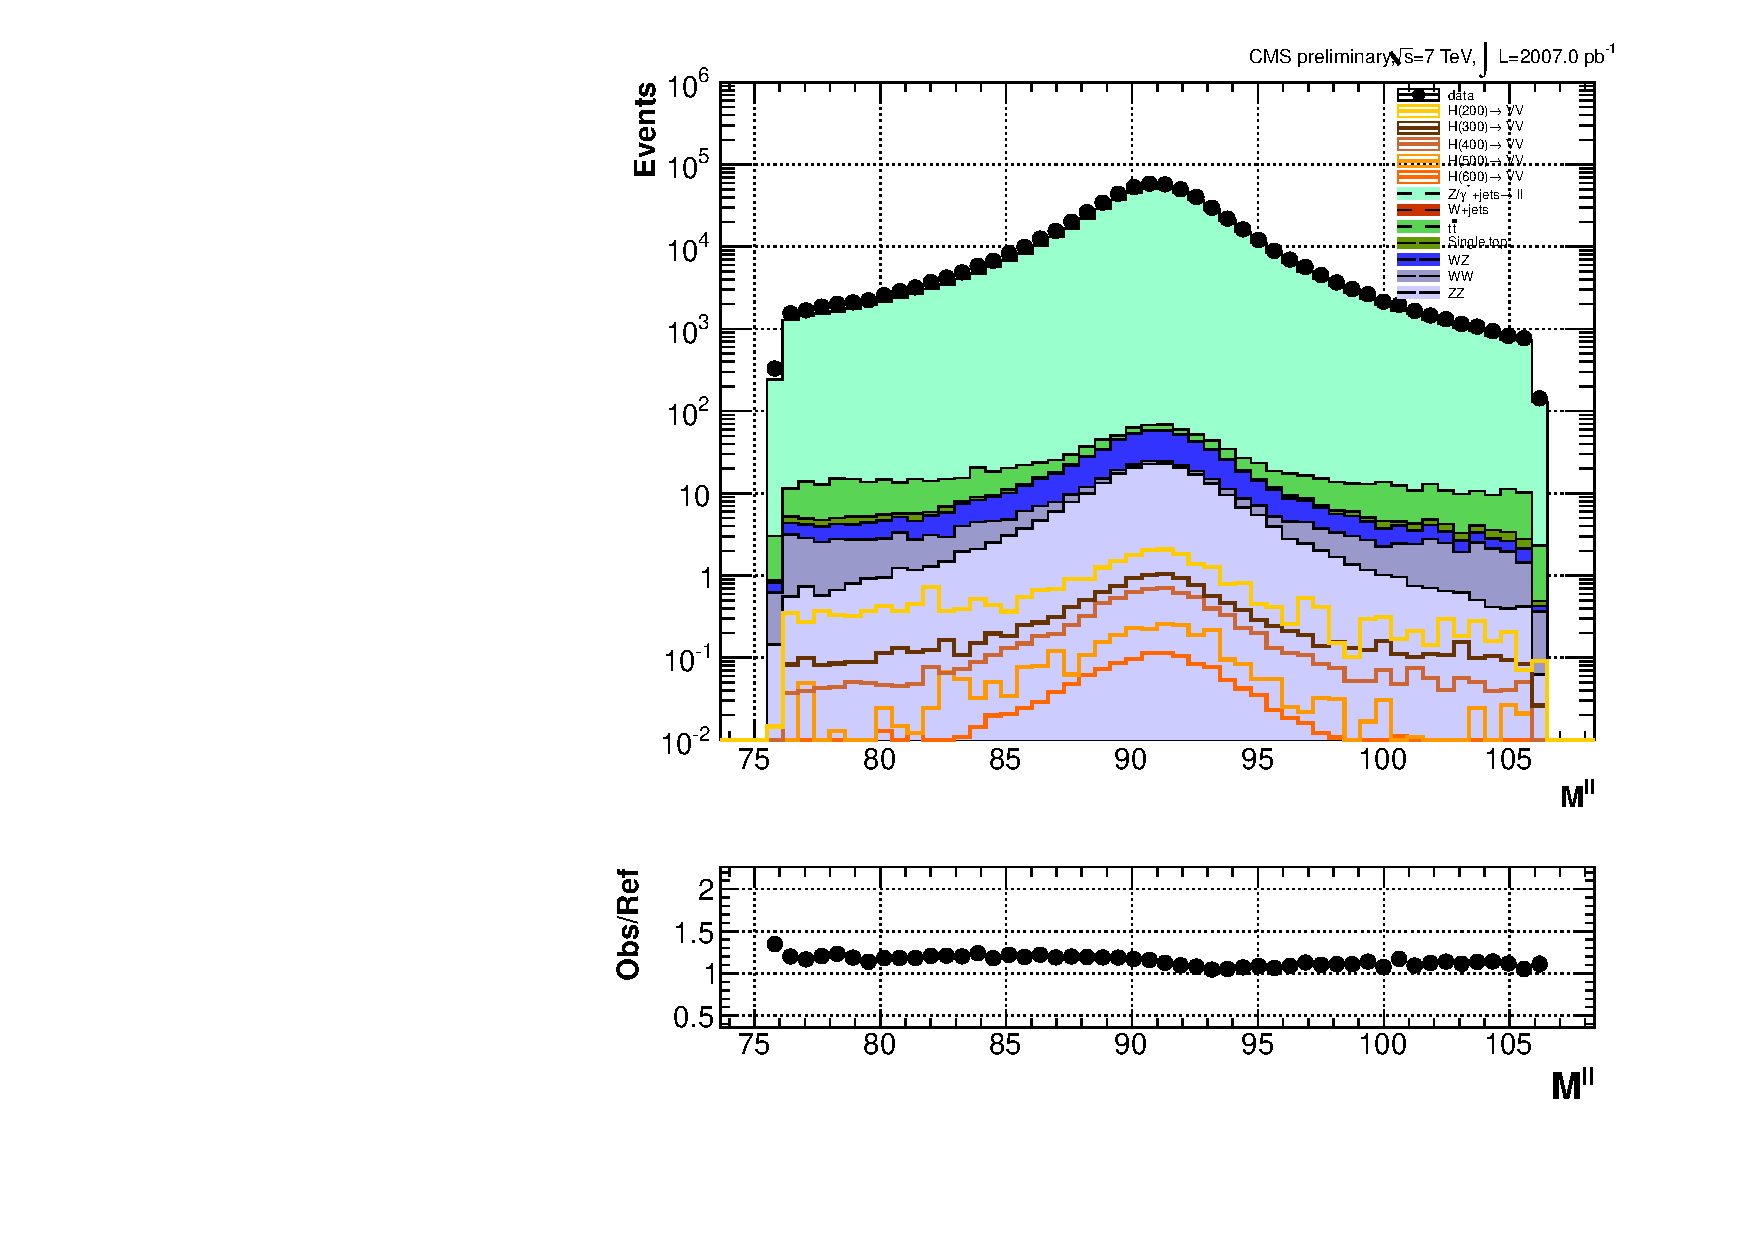
\includegraphics[width=0.4\textwidth]{img/mumu_recozmass}
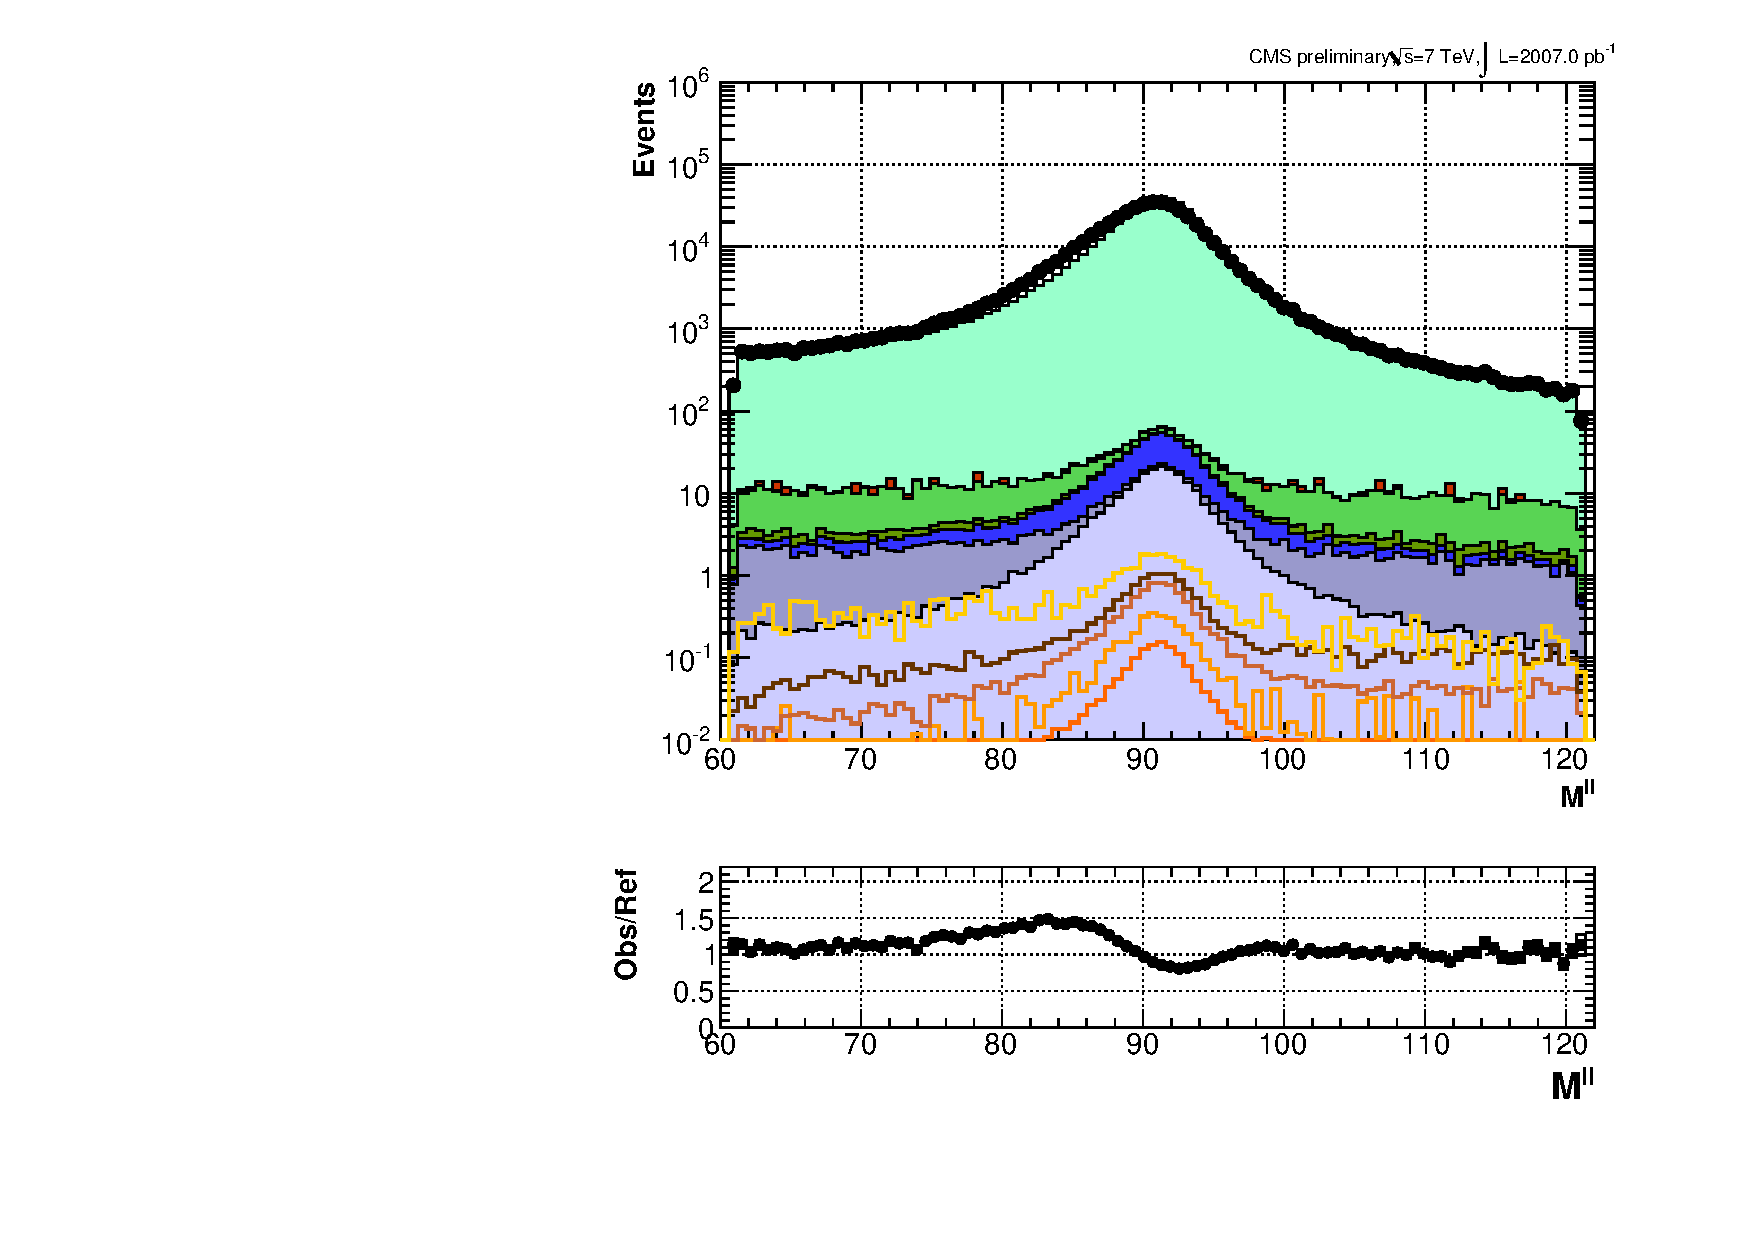
\includegraphics[width=0.4\textwidth]{img/ee_recozmass} \\
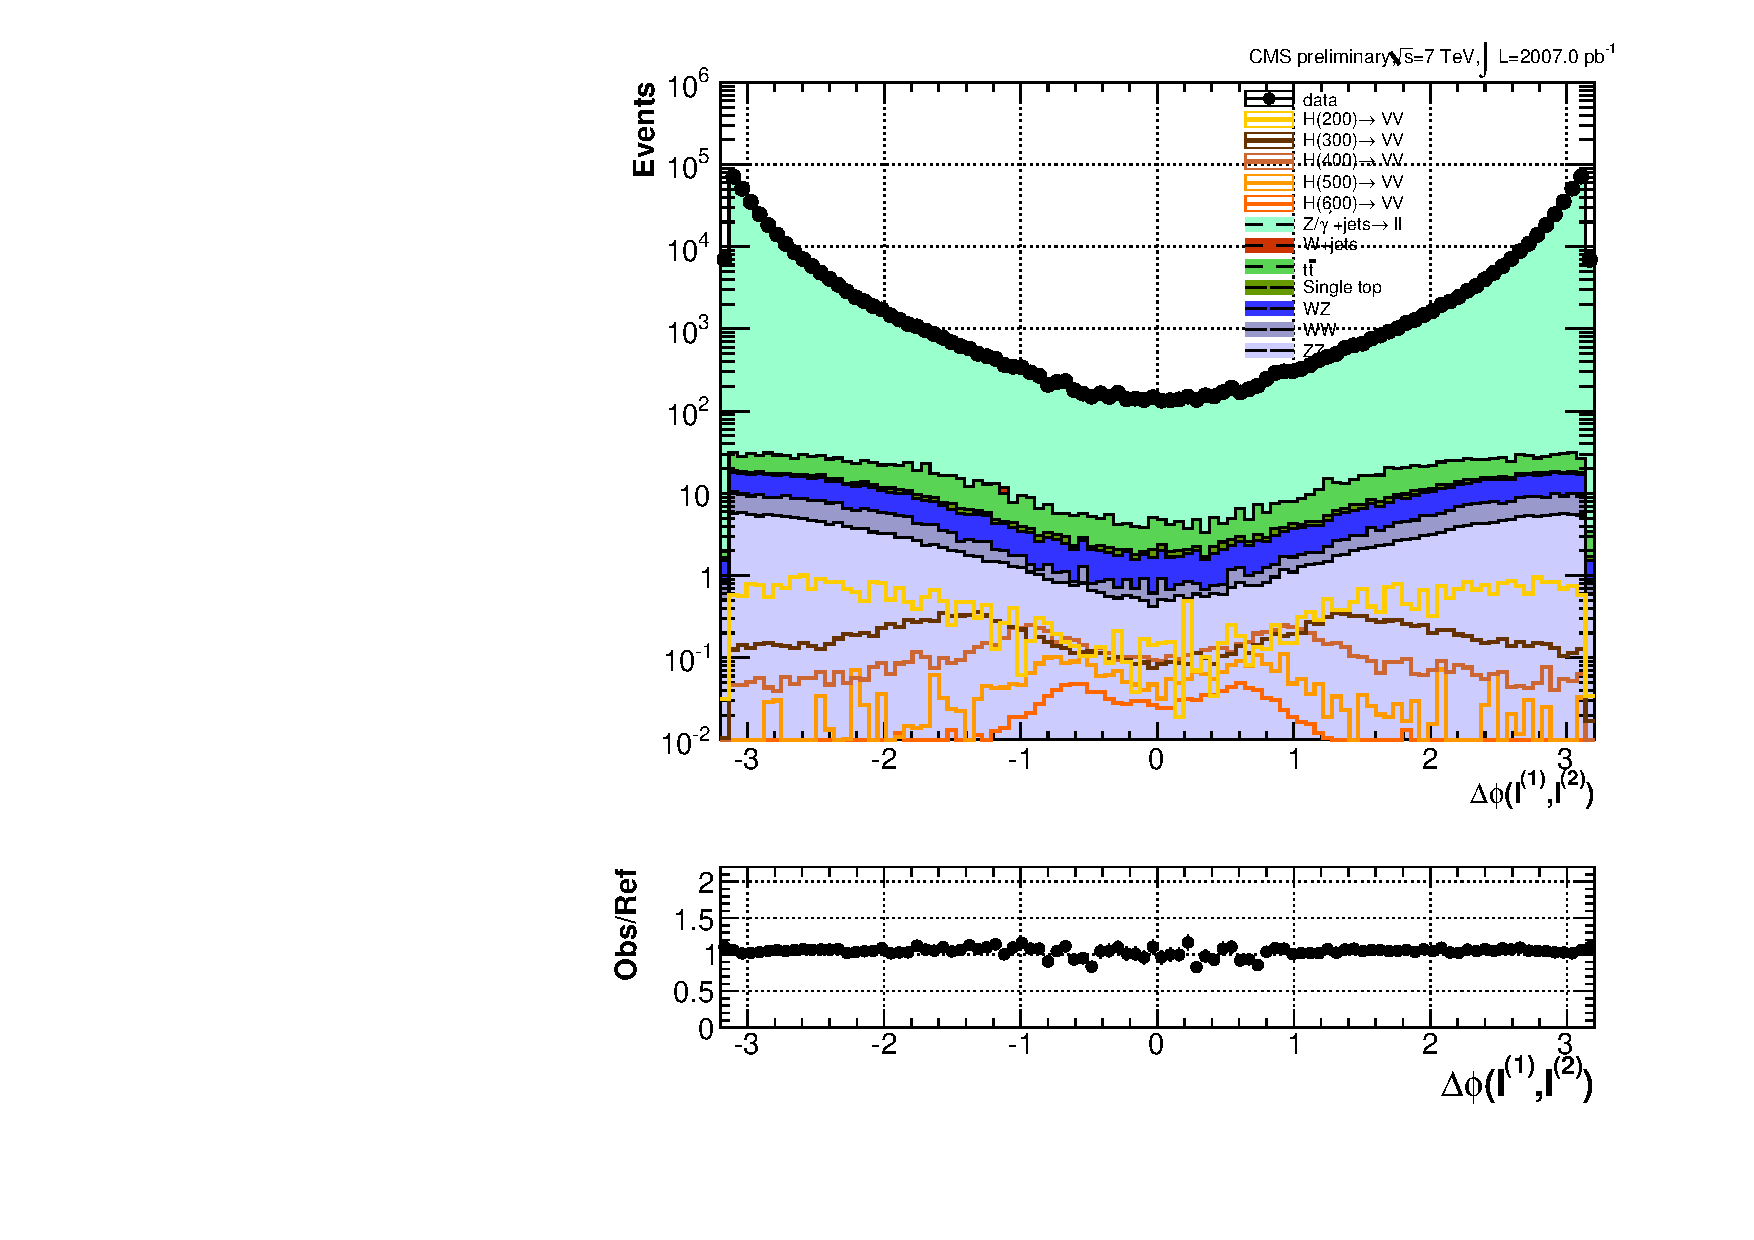
\includegraphics[width=0.4\textwidth]{img/mumu_recodphill}
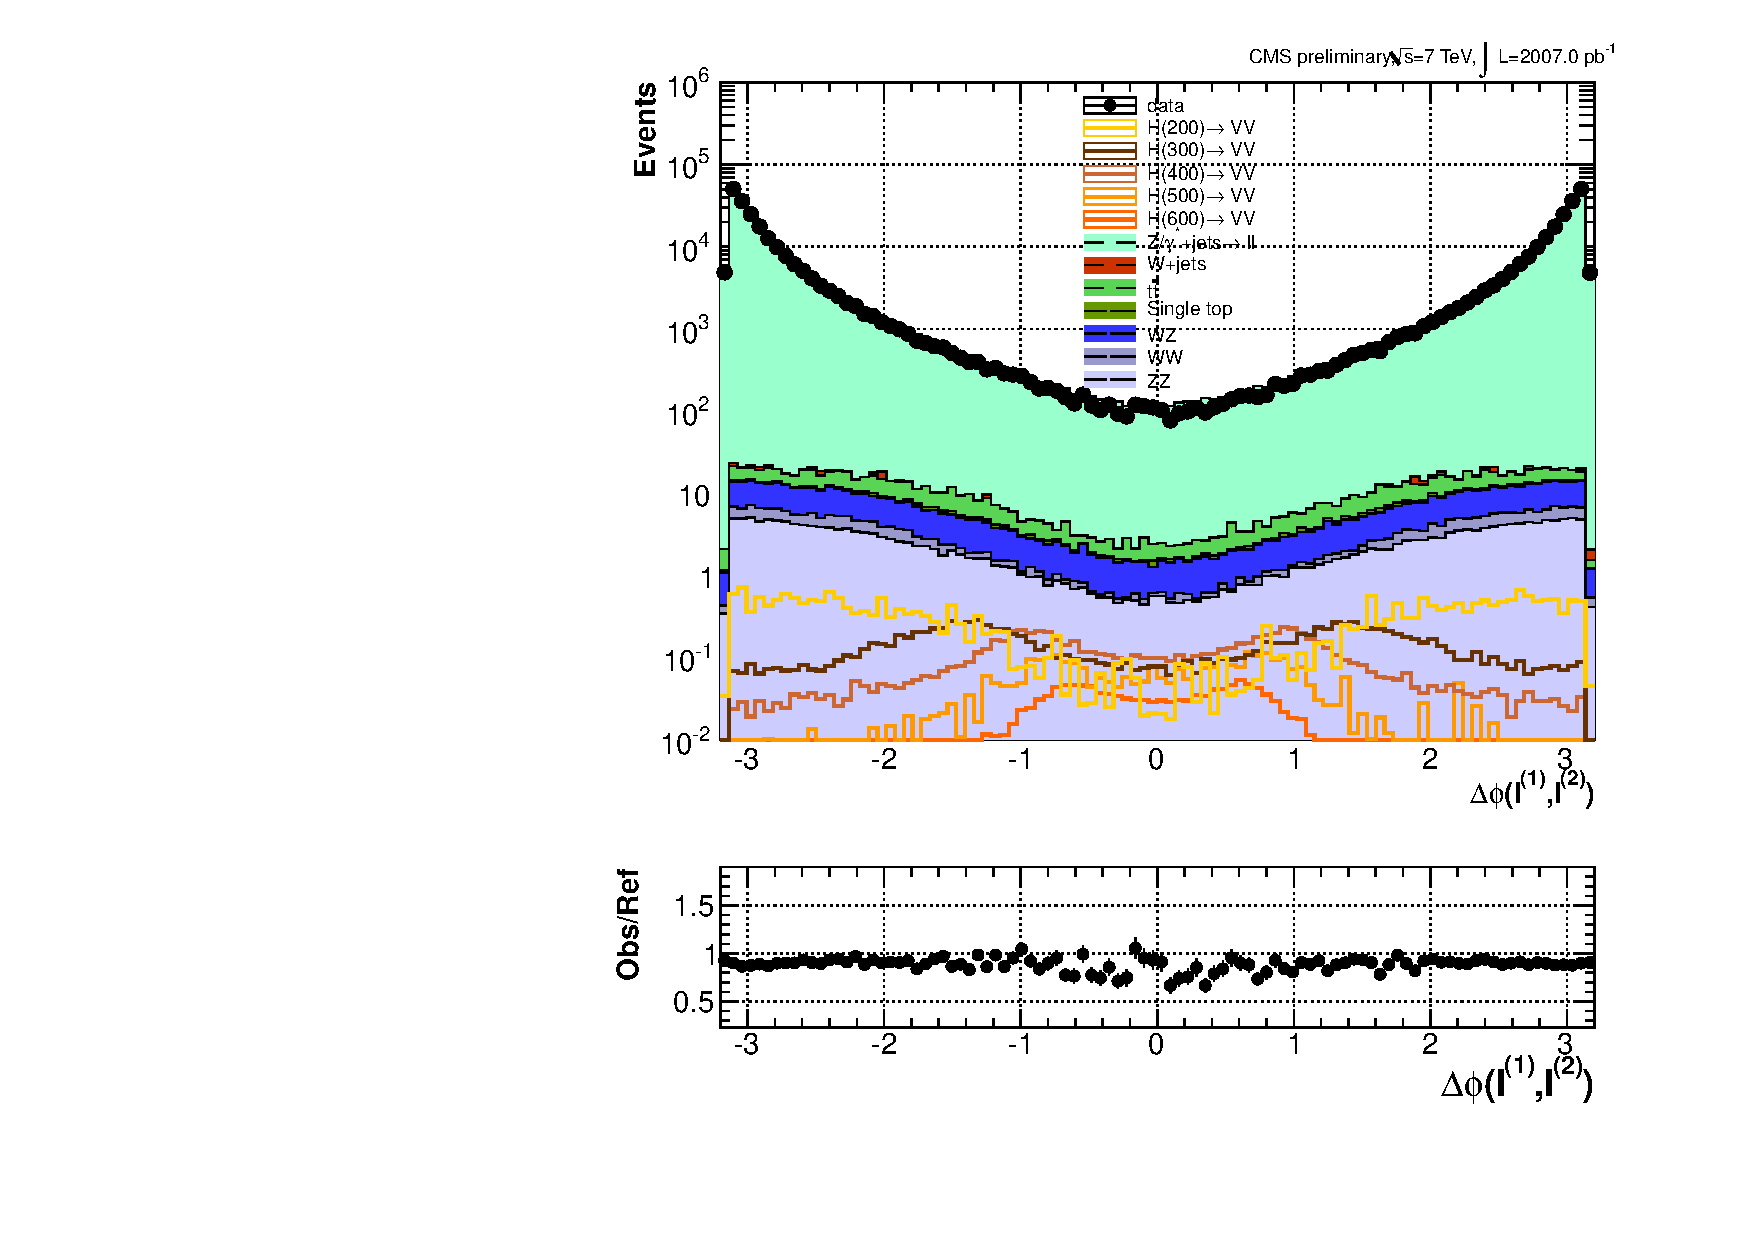
\includegraphics[width=0.4\textwidth]{img/ee_recodphill}
\caption{{\em Top}: dilepton invariant mass distribution for di-muon ({\em left}) and di-electron ({\em right}) events in a $\pm$30 GeV/c$^2$ acceptance window.
 with a mass compatible with the Z boson mass. {\em Bottom}: azimuthal angle between the two leading leptons.}
\label{fig:dileptoncontrol}
\end{center}
\end{figure}

In order to reduce the contamination from multilepton events, produced from WZ and ZZ decays,
events are vetoed if containing another loosely selected electron or muon as described above.
The loose selection applied on the third lepton is expected to have a high efficiency for signal events($>$99.8\% for both channels).
The remainder of WZ and ZZ events are mostly due to fully hadronic decays of one of the vector bosons or to the decay of a Z boson to neutrinos.
A slight excess of events with more than 2 muons is observed in data as shown in Fig~\ref{fig:thirdleptonveto}
most probably related to a higher lepton fake rate than the one modelled by the \MC.
Notice also that at this point no data-driven correction for the lepton efficiencies has been applied to correct further the \MC.

\begin{figure}[htp]
\begin{center}
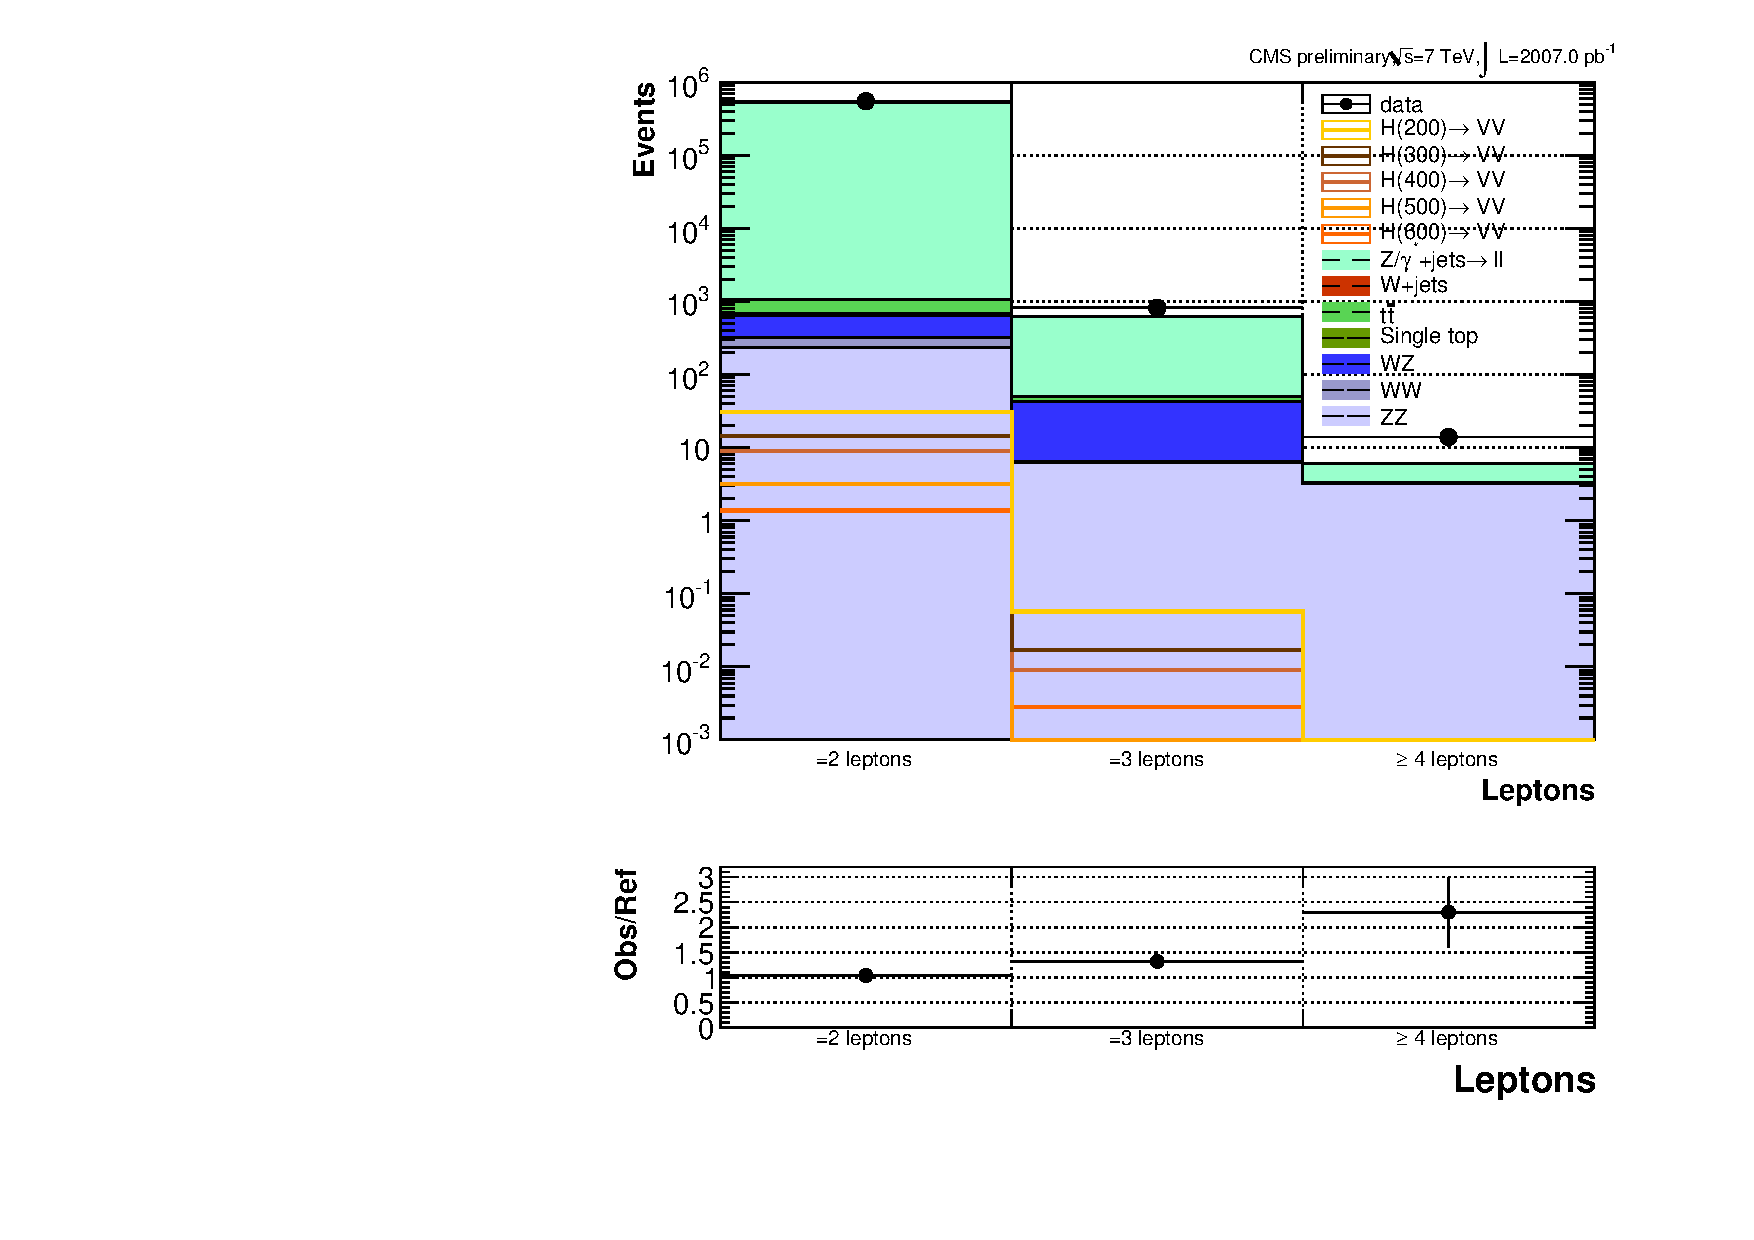
\includegraphics[width=0.4\textwidth]{img/mumu_nleptons}
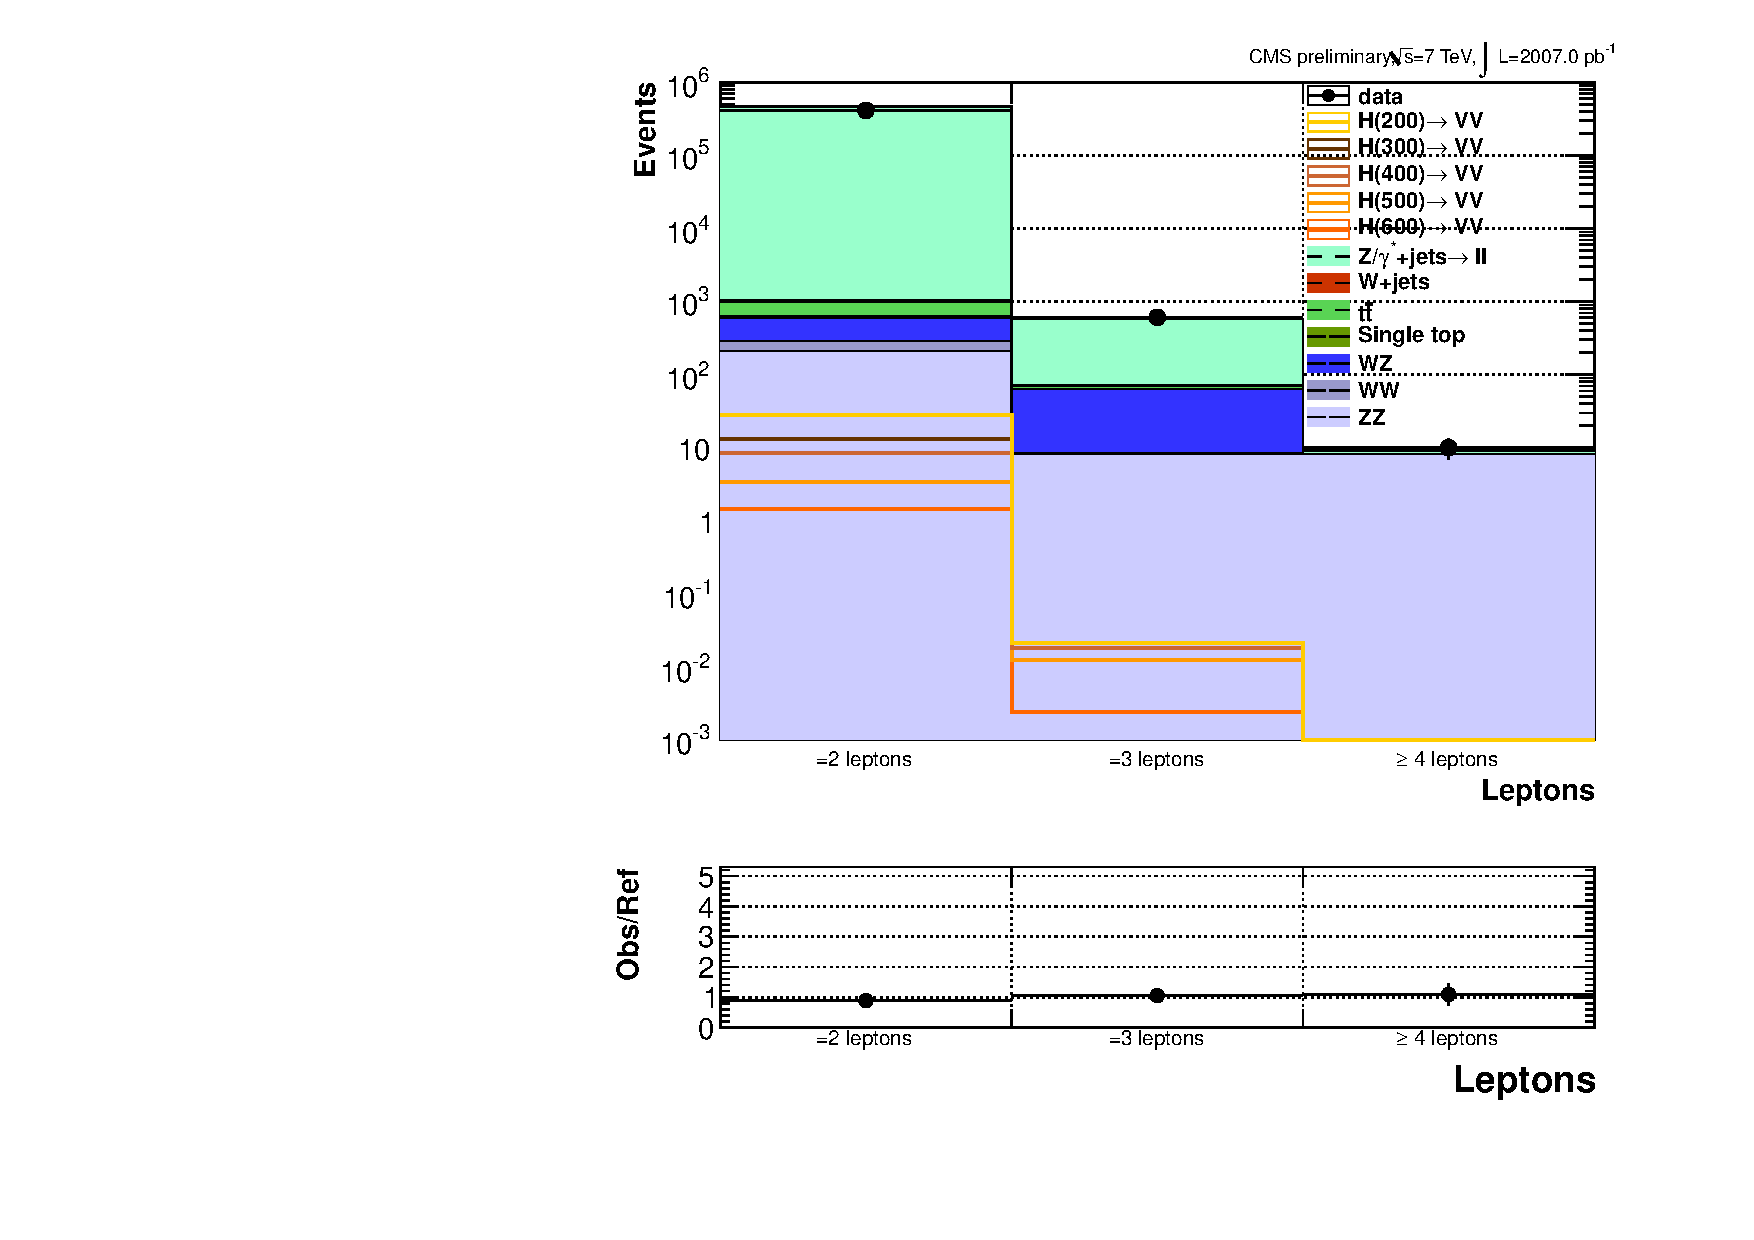
\includegraphics[width=0.4\textwidth]{img/ee_nleptons}
\caption{Lepton multiplicity distribution for di-muon ({\em left}) and di-electron ({\em right}) events with a mass compatible with the Z boson mass.}
\label{fig:thirdleptonveto}
\end{center}
\end{figure}


%%% JETS
\item[Jets] are reconstructed with the anti-$k_T$ algorithm with a cone of $R=0.5$ are selected with $p_T>$15~GeV/c and $|\eta|<5.0$.
The loose jet id used to select the jets is based on the electromagnetic fraction of the jets among other variables. 
The jet multiplicity distribution obtained after the dilepton selection is shown in Fig.~\ref{fig:jetmult} for jets found inside the tracker acceptance region only.
A good agreement is found between data and \MC prediction.

\begin{figure}[htp]
\begin{center}
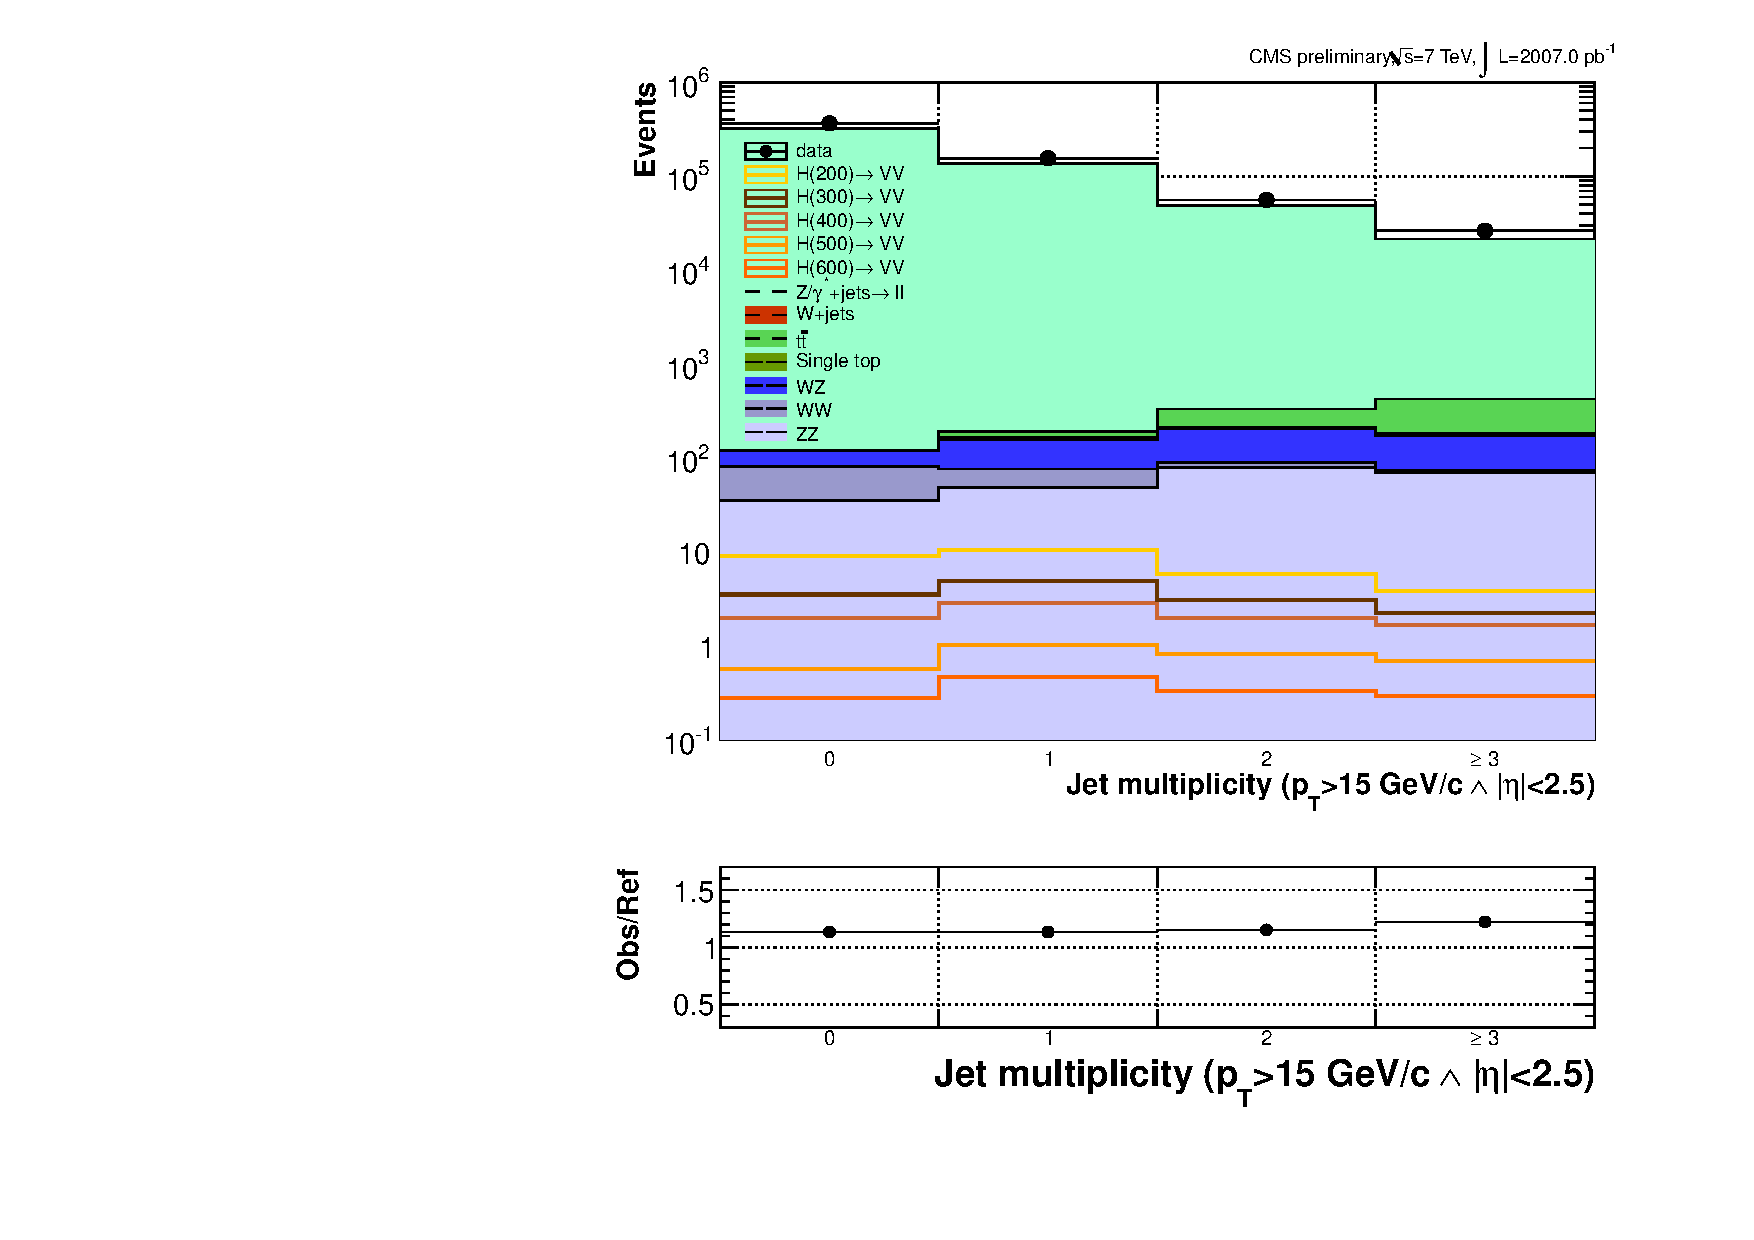
\includegraphics[width=0.4\textwidth]{img/mumu_njets}
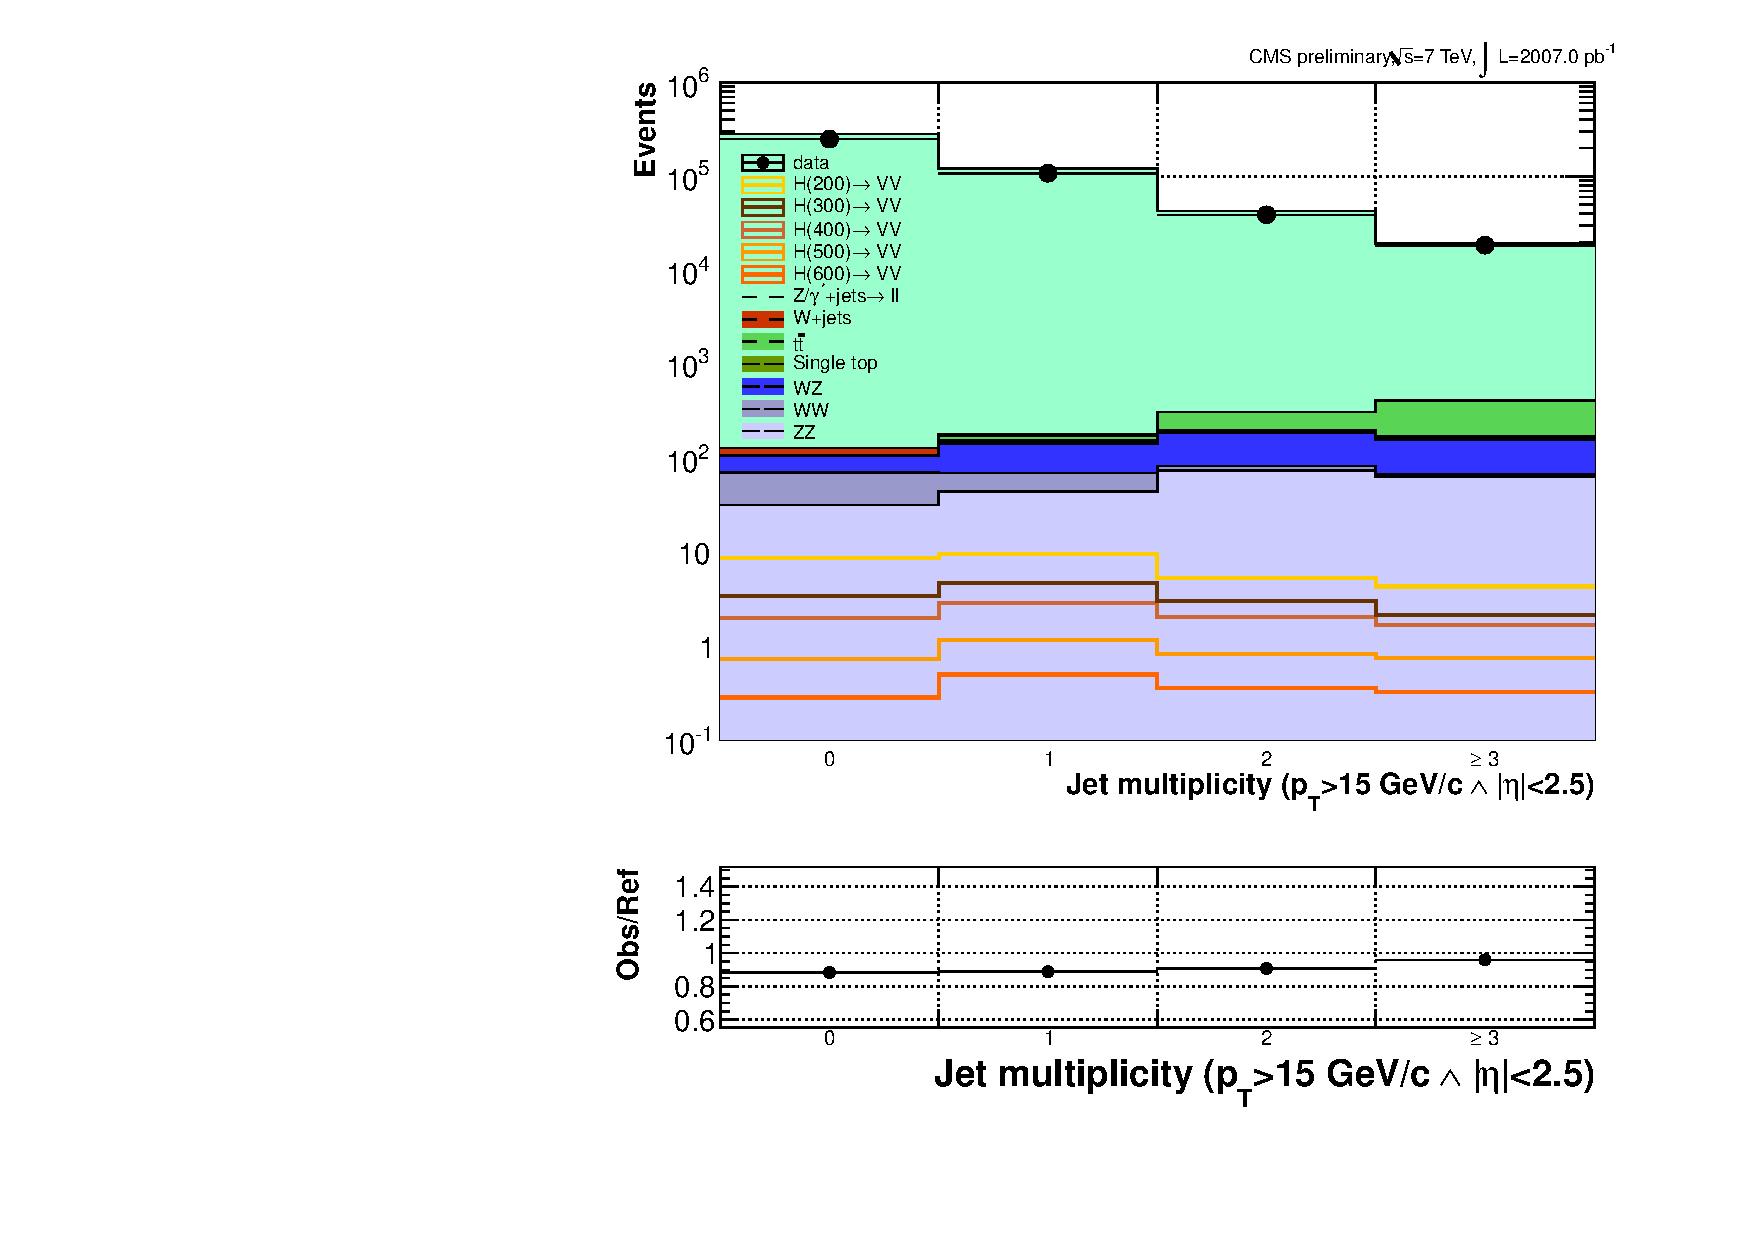
\includegraphics[width=0.4\textwidth]{img/ee_njets}
\caption{Jet multiplicity distribution in di-muon ({\em left}) and di-electron ({\em right}).}
\label{fig:jetmult}
\end{center}
\end{figure}

Jets with $|\eta|>$2.4 are used for analysis but not for for jet counting. In the forward region due to the limited acceptance of the tracker
no jet-vertex association is possible, and therefore, the contamination from pileup may become non negligible.
The effect can be estimated from simulation by considering the average jet multiplicity in $Z\rightarrow ll$ events
as a function of the generated pileup with and without the tracker acceptance requirement imposed.
The evolution of the average jest multiplicity as function of the pileup is shown in Fig~\ref{fig:jetmultvspu}, {\em left}.
We conclude that by restricting the acceptance of the jets used for counting to within the tracker acceptance region
minimizes the dependence on pileup, even if a small increase in the average multiplicity is expected.
The ratio of the multiplicity of two consecutive jet bins (e.g. $R_k=N_k/N_{k+1}$ with $k$=1,2,...),  
can also be used to evaluate the expected stability of jet counting
against the variation of the pileup scenario in data. In an ideal pileup-less scenario it is expected 
that $R_k$ is constant reflecting a ``staircase''-like jet multiplicity in $Z\rightarrow ll$ events.
This structure results from the fact that the jets are mainly generated from initial state radiation (ISR).
The distributions for different $R_k$ are shown in Fig~\ref{fig:jetmultvspu}, {\em right}.
It is observed that restricting  the acceptance of the jets for counting to the tracker acceptance region
stabilizes the value of $R_k$ independently of the pileup scenario, yielding a jet multiplicity
closer to the ideal ``staircase'' distribution where $R_k=$cte.
For processes where jets are generated from decays with flux of color or where jets accompany the fusion of heavy objects
like W/Z vector bosons (i.e. VBF processes), $R_k$ is no longer constant and reflects a ``Poisson''-like jet multiplicity~\cite{Englert:2011pq}.
As the VBF signature constitutes, per se, a distinct production process of the Higgs boson, it is important
to identify correctly this transition in the jet multiplicity by reducing the contamination from pileup.
VBF jets will also tend to be forward motivating the usage of jets reconstructed at high pseudo-rapidty.
These arguments support our choice to count jets inside the tracker acceptance region only
and used jets at higher $\eta$ regions for the purpose of identifying VBF like processes. 
The VBF specific selection will be discussed in more detail in Sec.~\ref{sec:higgssearch}.

\begin{figure}[htp]
\begin{center}
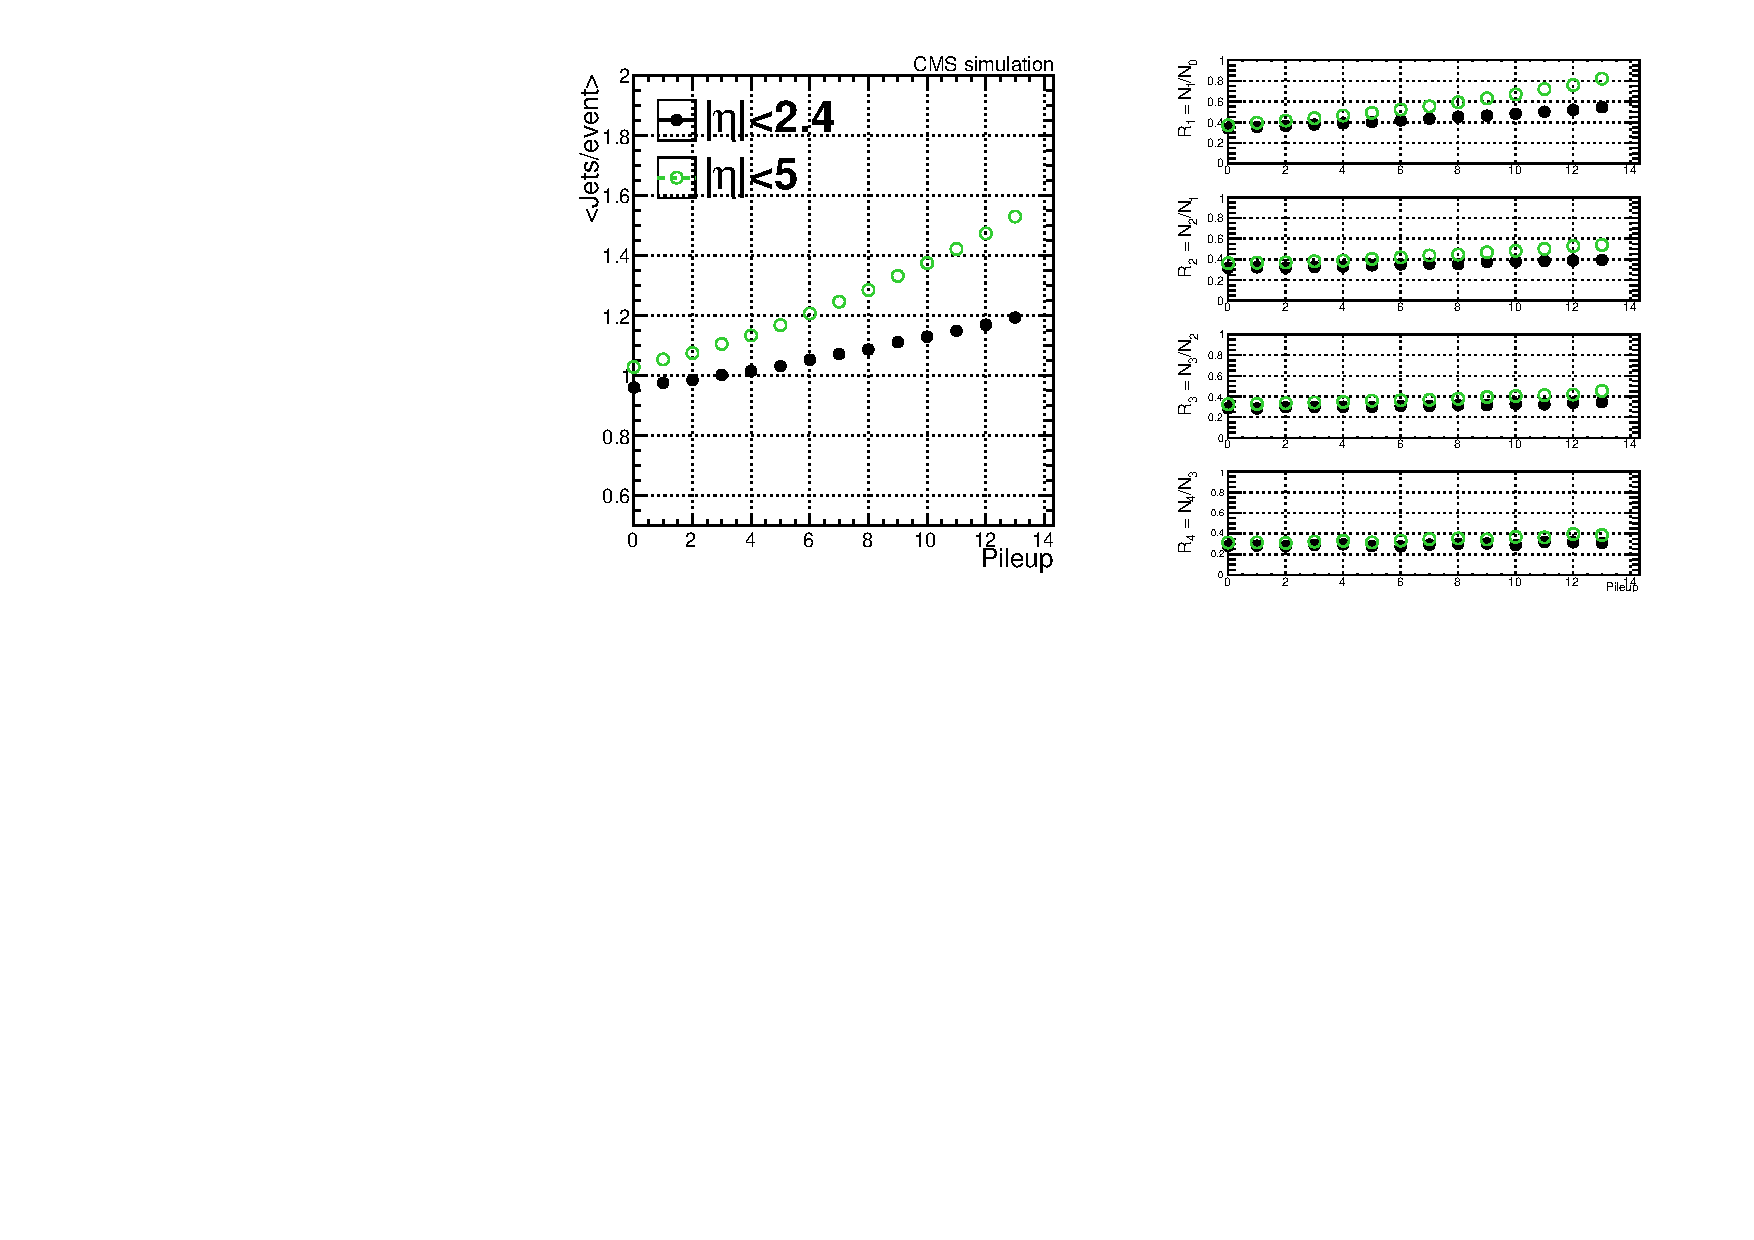
\includegraphics[width=0.9\textwidth]{img/dy_jetmultvspu}
\caption{Evolution of the average jet multiplicity ({\em left}) and the ratio of consecutive jet multiplicity bins ({\em right})
as function of the generated pileup in $Z\rightarrow ll$ events. 
Two cases are superimposed on each plot for comparison: 
jets in the central region ($|\eta|<$2.4) and all reconstructed jets ($|\eta|<$5.0).}
\label{fig:jetmultvspu}
\end{center}
\end{figure}

In order to reduce the contamination from processes which produce heavy flavor jets such as \ttbar, single top, vector boson + heavy quarks production, b-tagging algorithms are used.
The jet-B probability (JBP) and the simple secondary vertex high efficiency (SSVHE) taggers are used for this purpose. 
Details of these algorithms and their performance can be found in~\cite{CMS-PAS-BTV-11-002}. The JBP algorithm is chosen
as it is expected to provide the highest efficiency in \ttbar events for a mistag rate of 10\% (loose working point).
The SSVHE tagger is used to complement the JBP tagger as it is designed for higher purity of $b$-jet identification and can therefore
increase the $b$-tagging efficiency without leading to a significant increase of the mistag rate. 
Events with a jet with $p_T>$30~GeV/c, tagged with the loose working point of the JBP algorithm or with the medium working point of the SSVHE algorithm, are rejected. 
This choice is made after optimizing the efficiency of the rejection of the top contribution as summarized in Tab.~\ref{tab:btagoptim}.
Fig.~\ref{fig:btagging} shows the b-tag multiplicity distributions observed in di-muon and di-electron events using the combination of taggers just described.
A good agreement, within 10-15\% is found between data and \MC taking into account that at this point no data-driven correction scale factors for the $b$-tag and mistag rates have been applied.
The level of discrepancy observed is in fact compatible with the $\approx$ 10\% scale factor measured for the mistag rate~\cite{CMS-PAS-BTV-11-002}.
The usage of the data-derived scale factors for the $b$-tagging algorithms will be discussed in more detail in Sec.~\ref{subsec:systunc}.

\begin{table}[htp]
\caption{b-tag optimization using different algorithms and different combinations.
Top refers to the residual number of events expected from \ttbar and single top production.
Higgs refers to the number of events surviving the $b$-tagging veto for a mass of 200~GeV/c$^{2}$.
The yields include the di-muon and the di-electron channels for an integrated luminosity of 2007~pb$^{-1}$.
The last line shows the signal/background ratio used to optimize the choice of the $b$-tagging algorithm.
The taggers compared are Track Counting High Efficiency (TCHE), Jet B-probability (JBP) and Simple Secondary Vertex High Efficiency (SSVHE).
Two suffixes used for the different taggers denote the Loose and Medium working points.}
\label{tab:btagoptim}
\begin{center}
\begin{tabular}{lccccc} \hline\hline
\multirow{2}{*}{Process} & \multicolumn{5}{c}{Events accepted} \\
              & TCHEL          & JBPL      & SSVHEM   & TCHEL or SSVHEM & JBPL or SSVHEM \\\hline
Top           & 124.03         & 107.95    & 230.22   & 108.60          & 102.1          \\
Higgs (200)   & 50.97          & 51.97     & 55.31    & 50.74           & 51.77          \\\hline
S/B           & 0.41           & 0.48      & 0.24     & 0.47            & 0.51           \\
\hline\hline
\end{tabular}
\end{center}
\end{table}


\begin{figure}[htp]
\begin{center}
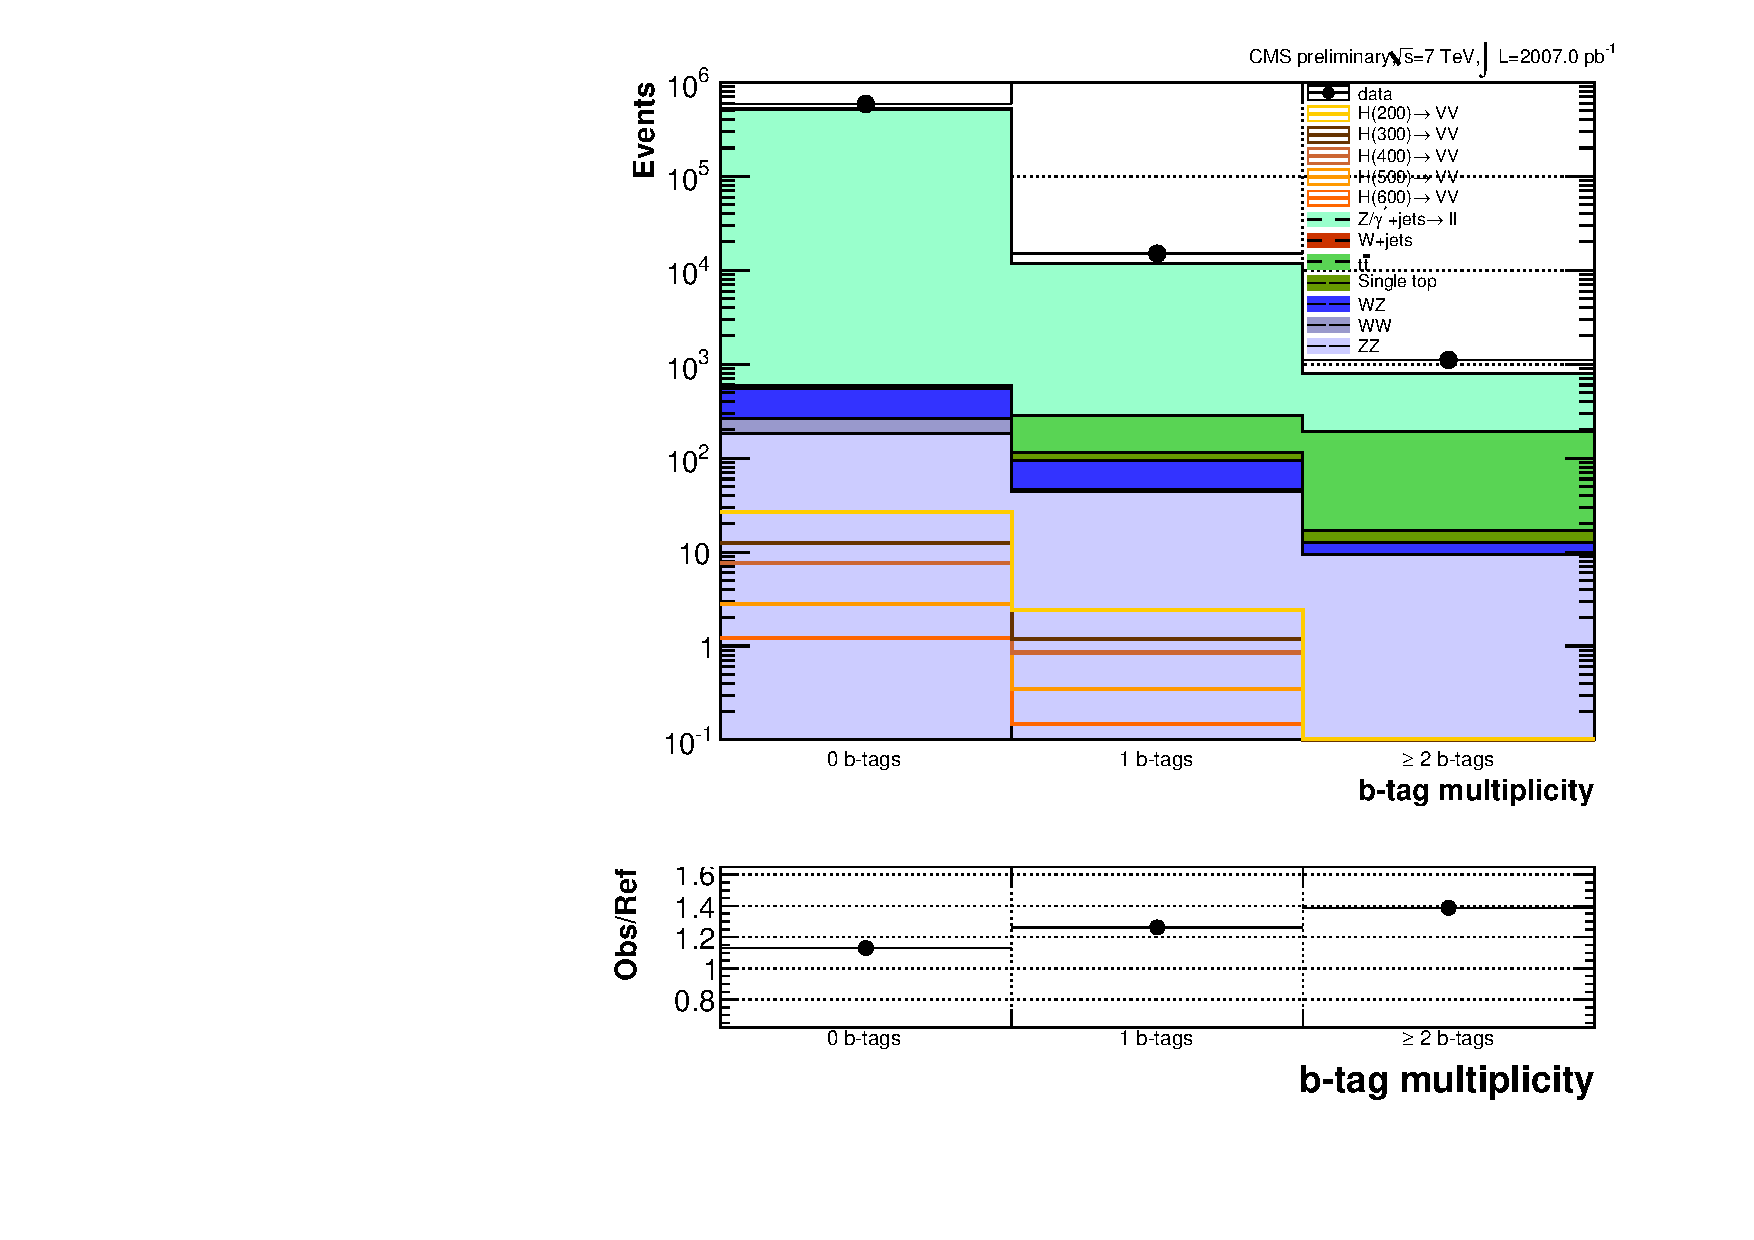
\includegraphics[width=0.46\textwidth]{img/mumu_nbtags}
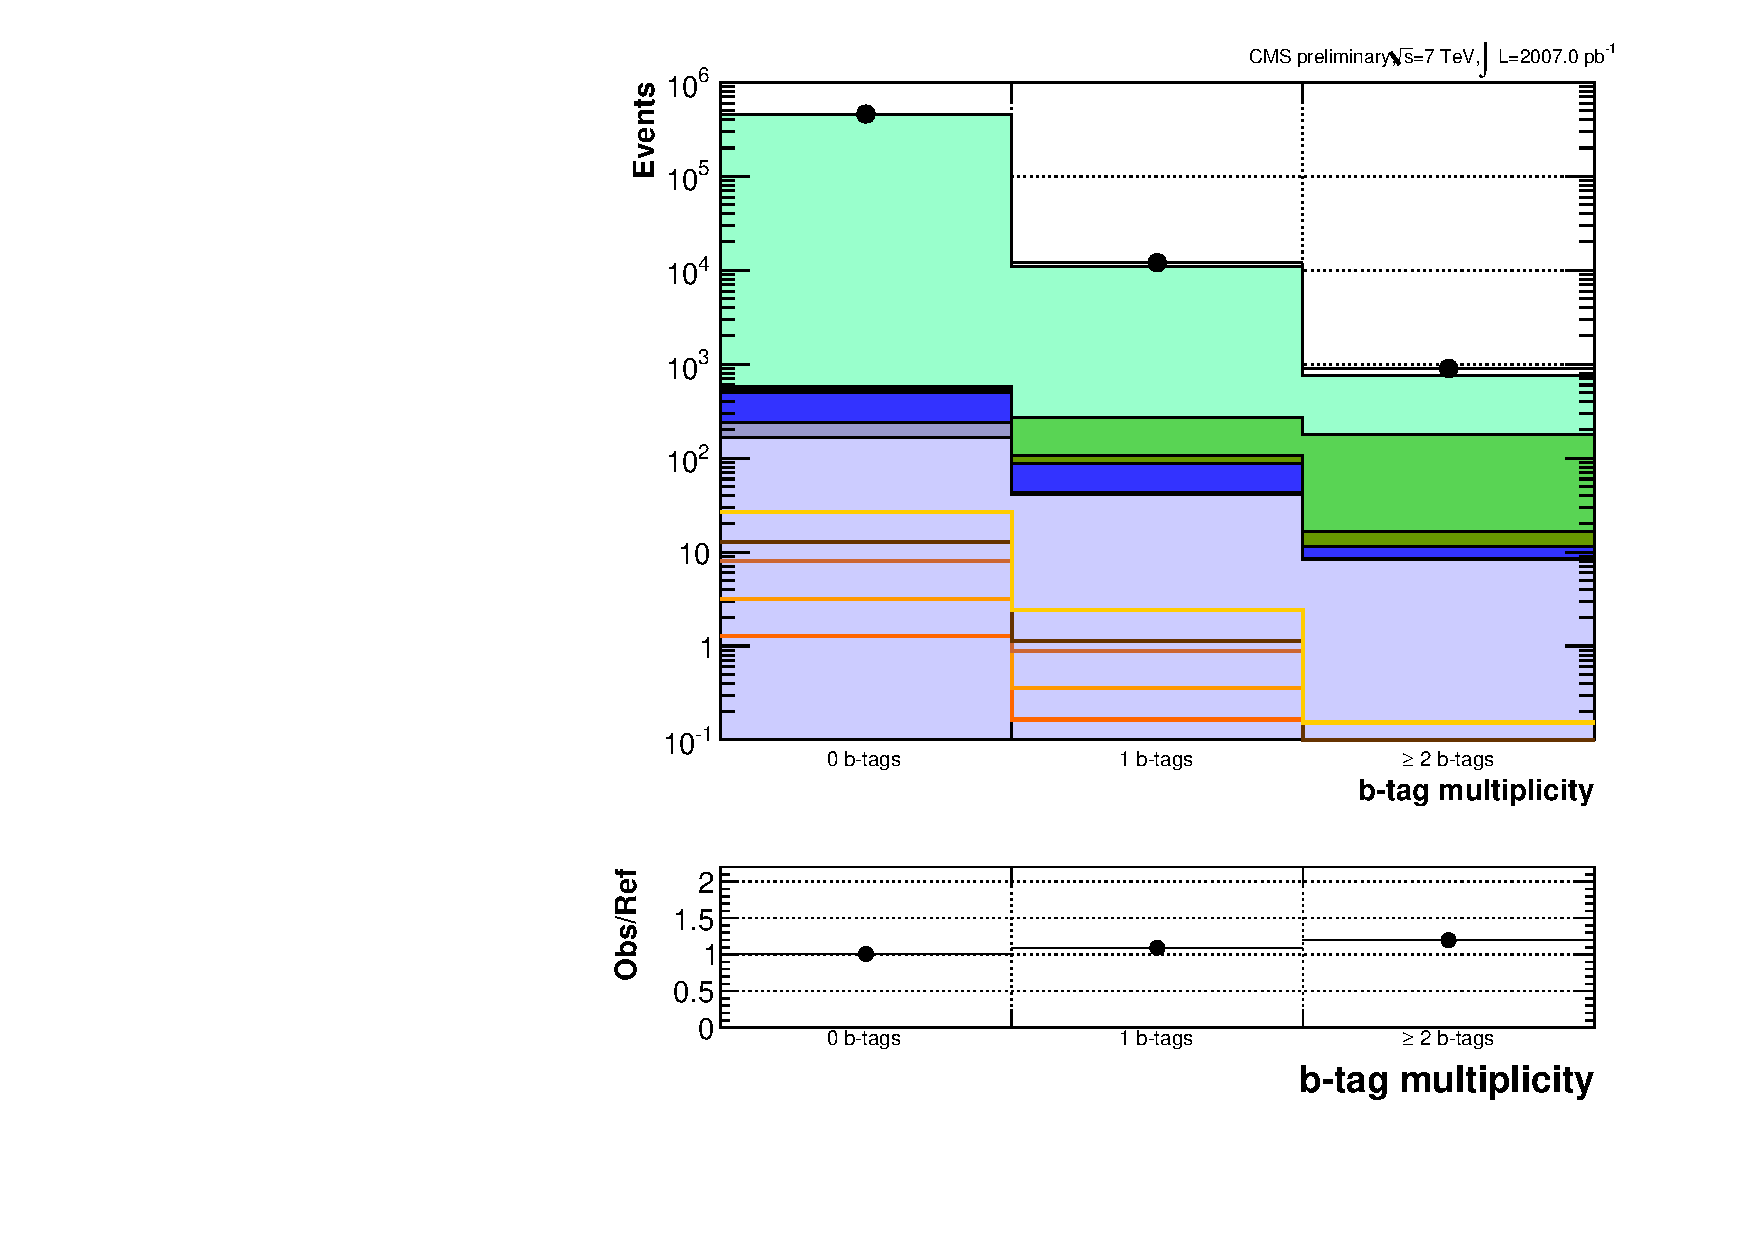
\includegraphics[width=0.46\textwidth]{img/ee_nbtags}
\caption{b-tag  multiplicity distribution in di-muon ({\em left}) and di-electron ({\em right}).}
\label{fig:btagging}
\end{center}
\end{figure}

%%% VBF
\item[Vector Boson Fusion]:  The identification of the events produced via Vector Boson Fusion (VBF) is based on the presence in the event of two leading jets in the forward regions of with an invariant mass of at least $450~GeV/c$ and a $\Delta\eta$-gap$>3.5$.
In addition, these two jets must not be identified as b-jets.
In order to reduce the potential impact of the pile-up on, only jets with $p_T>30~GeV/c$ are considered.
Presence of additional jets ($p_T>15~GeV/c$) in the tracker acceptance is also forbidden.
Finally, the two legs of the dilepton must be conained between the two leading jets.
Fig.~\ref{fig:vbfdEta} shows the distribution of the $\eta$-gap between the two VBF jets while Fig.~\ref{fig:vbfiMass} shows the distribution of the invariant mass between the two VBF jets. 
The fraction of simulated background dilepton events (with $|M-M_Z|<$15~GeV/c) being tagged as VBF events is about $4.0\times10^{-4}$, while the selection efficiency is about 25-30\% for Higgs produced via vector boson fusion in the mass range [200-600]~GeV/c$^{2}$ as shown on Fig.~\ref{fig:vbfeventflow}.

\begin{figure}[htp]
\begin{center}
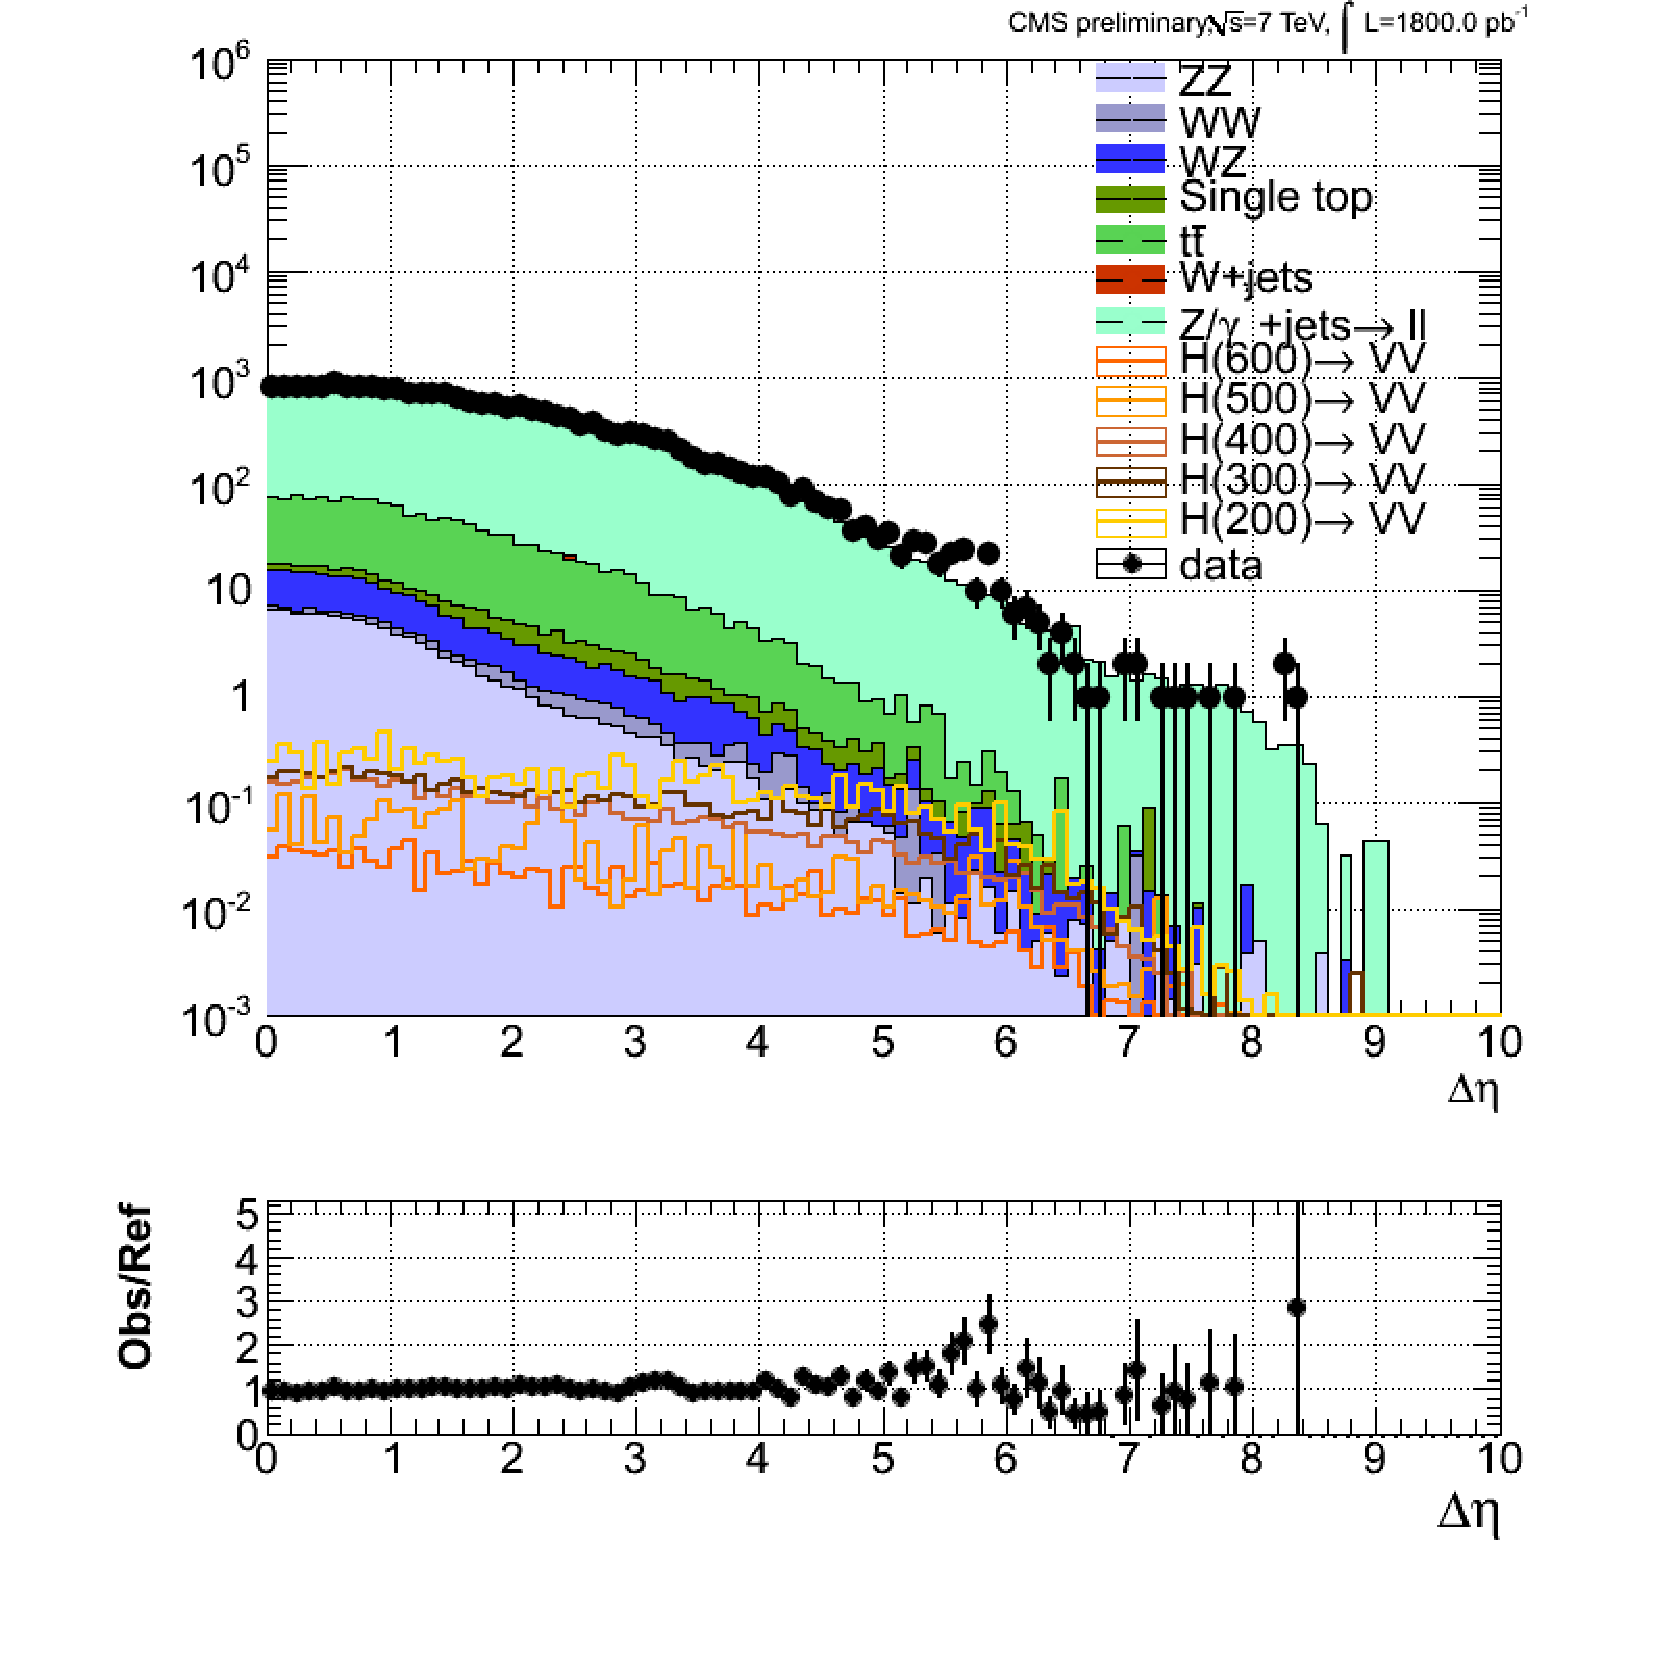
\includegraphics[width=0.46\textwidth]{img/mumu_VBFdEta}
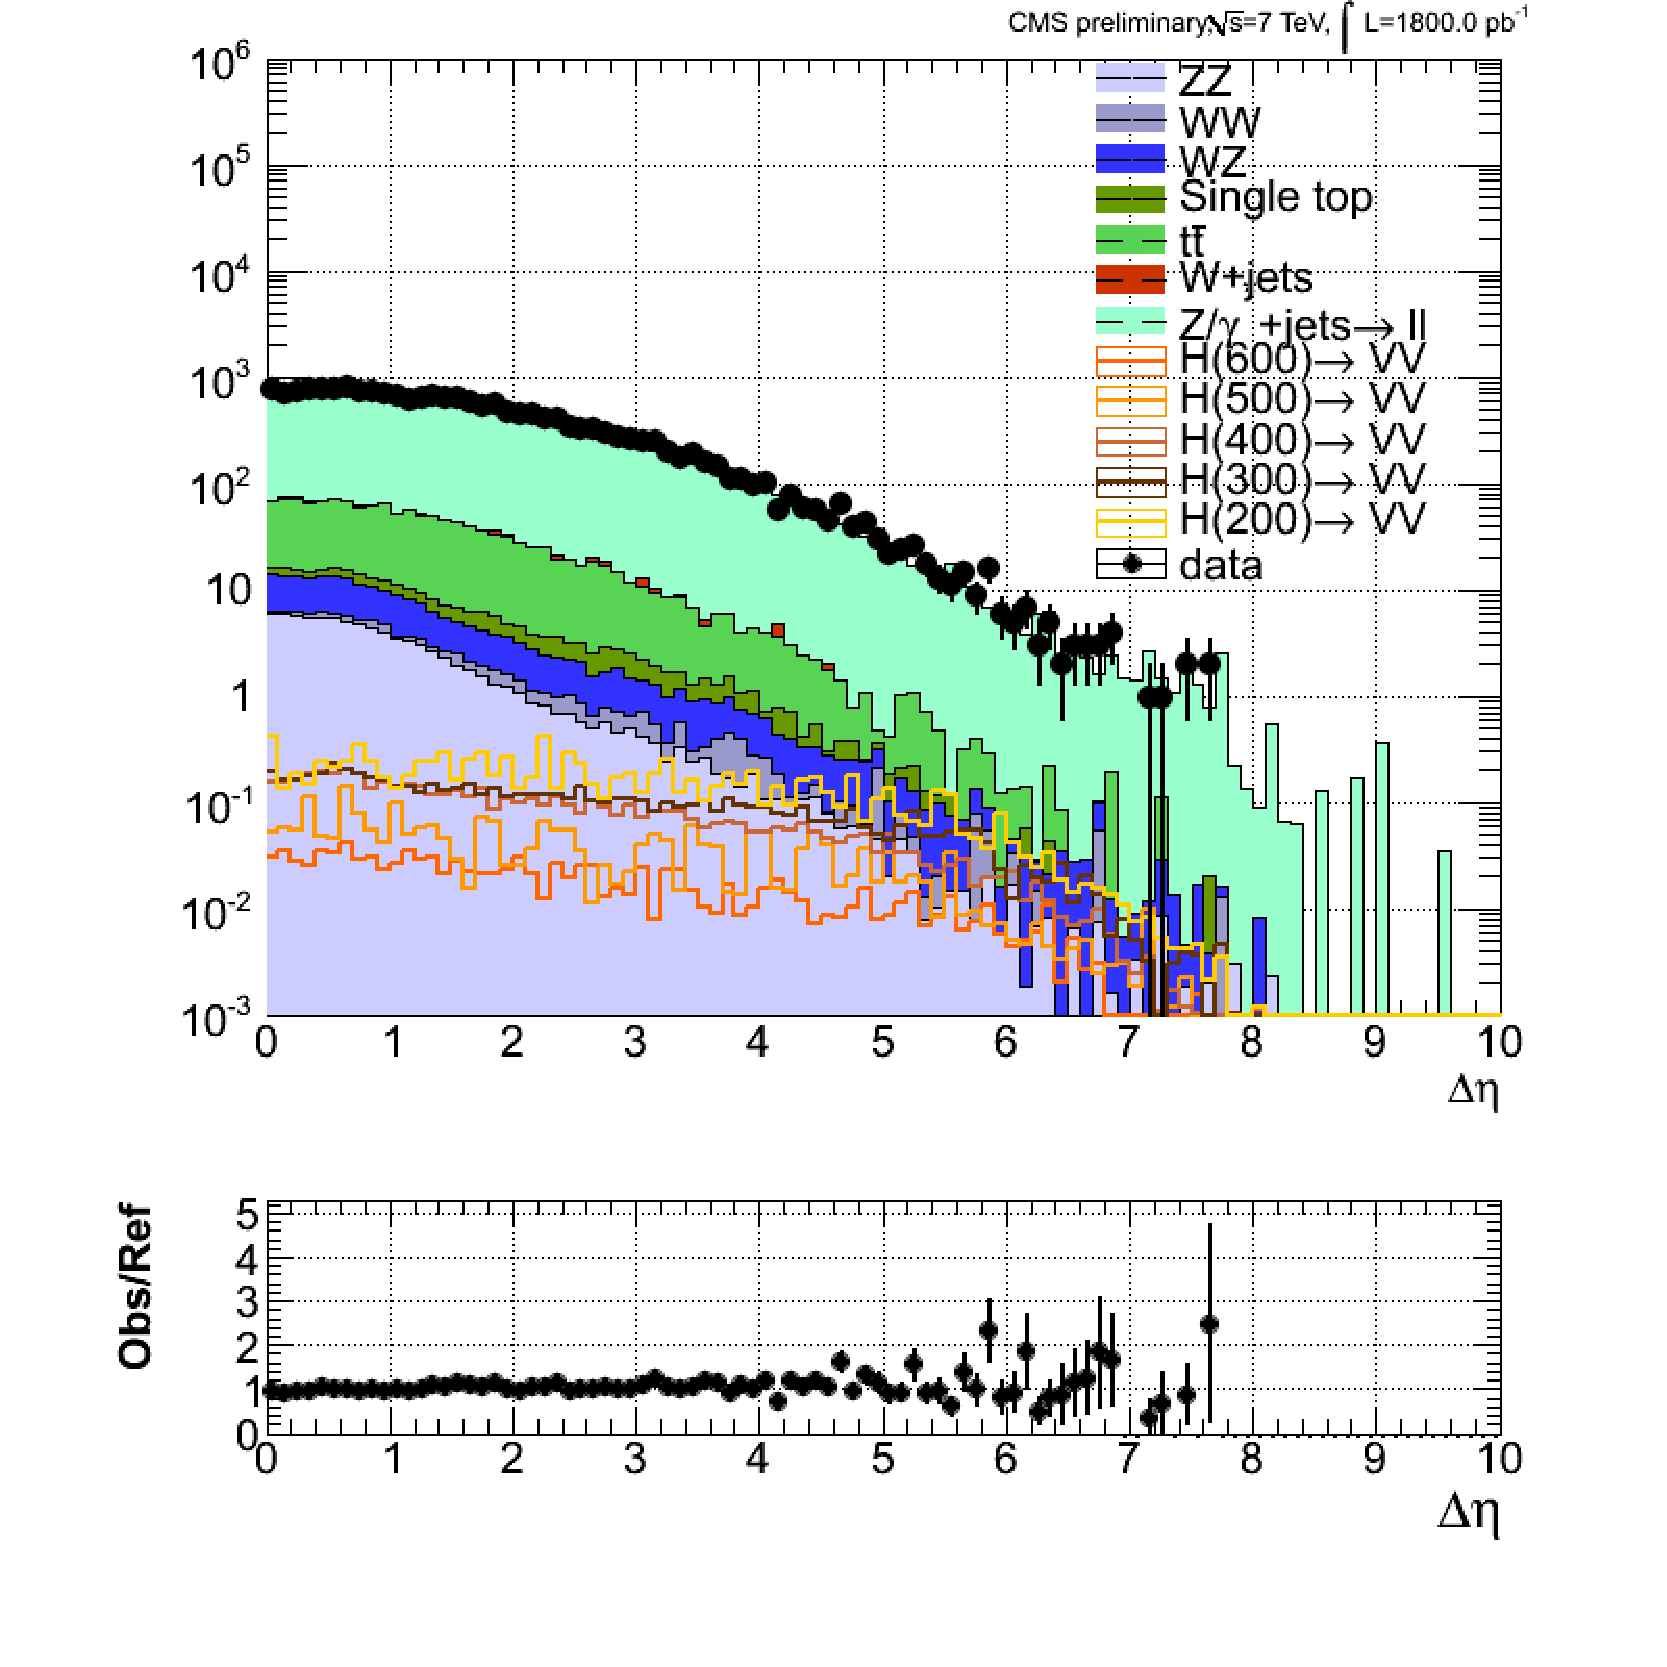
\includegraphics[width=0.46\textwidth]{img/ee_VBFdEta}
\caption{Distribution of $\Delta\eta$ between the two VBF jets in di-muon ({\em left}) and di-electron ({\em right}).  Note that signal is populated only with VBF produced Higgs.}
\label{fig:vbfdEta}
\end{center}
\end{figure}

\begin{figure}[htp]
\begin{center}
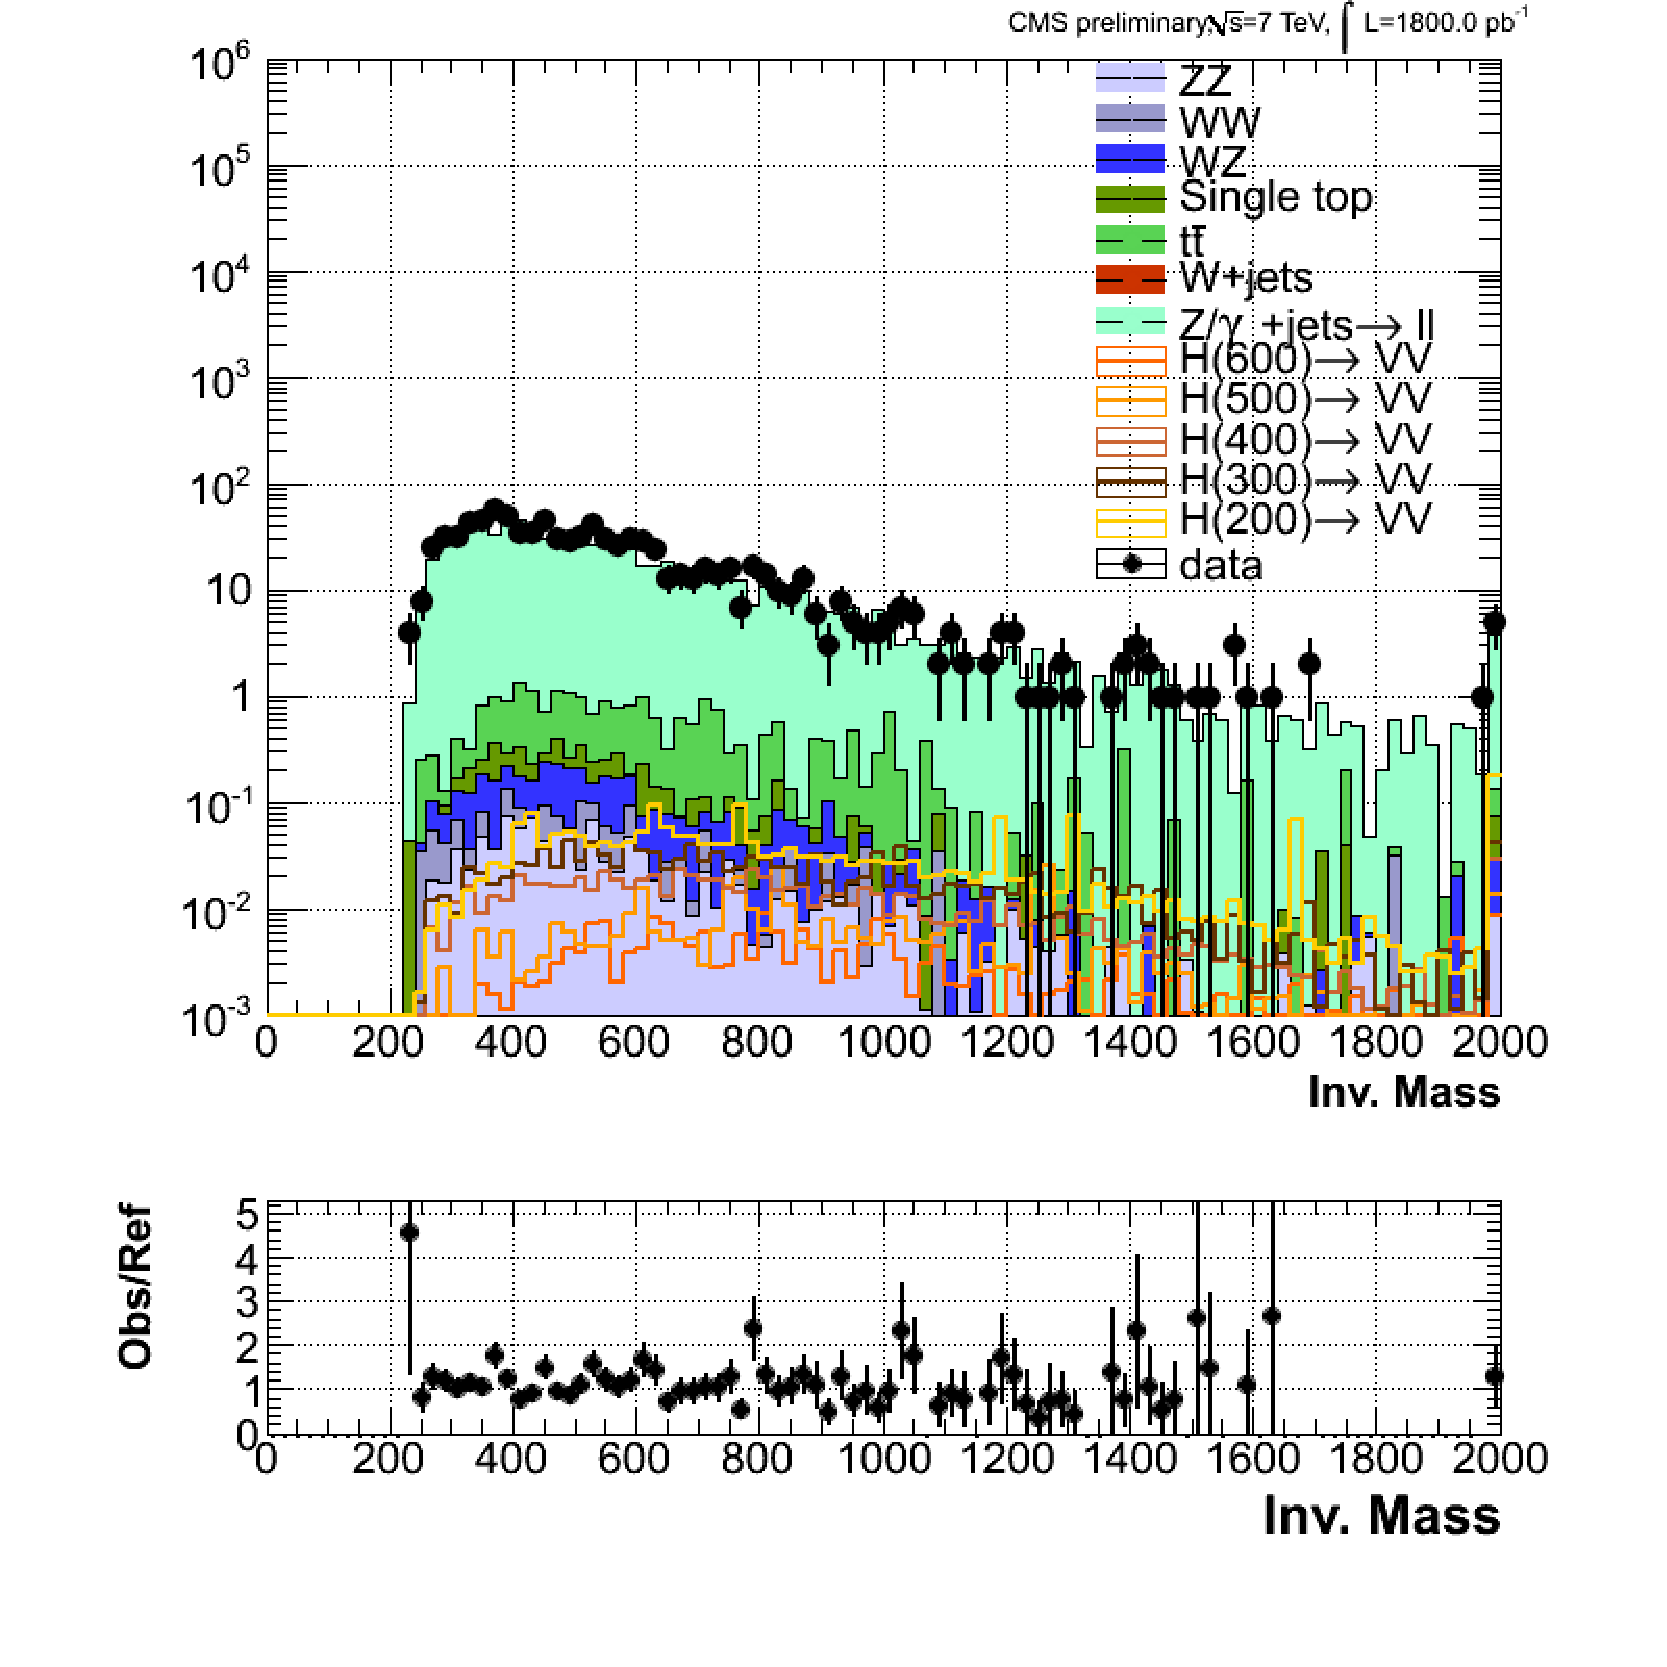
\includegraphics[width=0.46\textwidth]{img/mumu_VBFiMass}
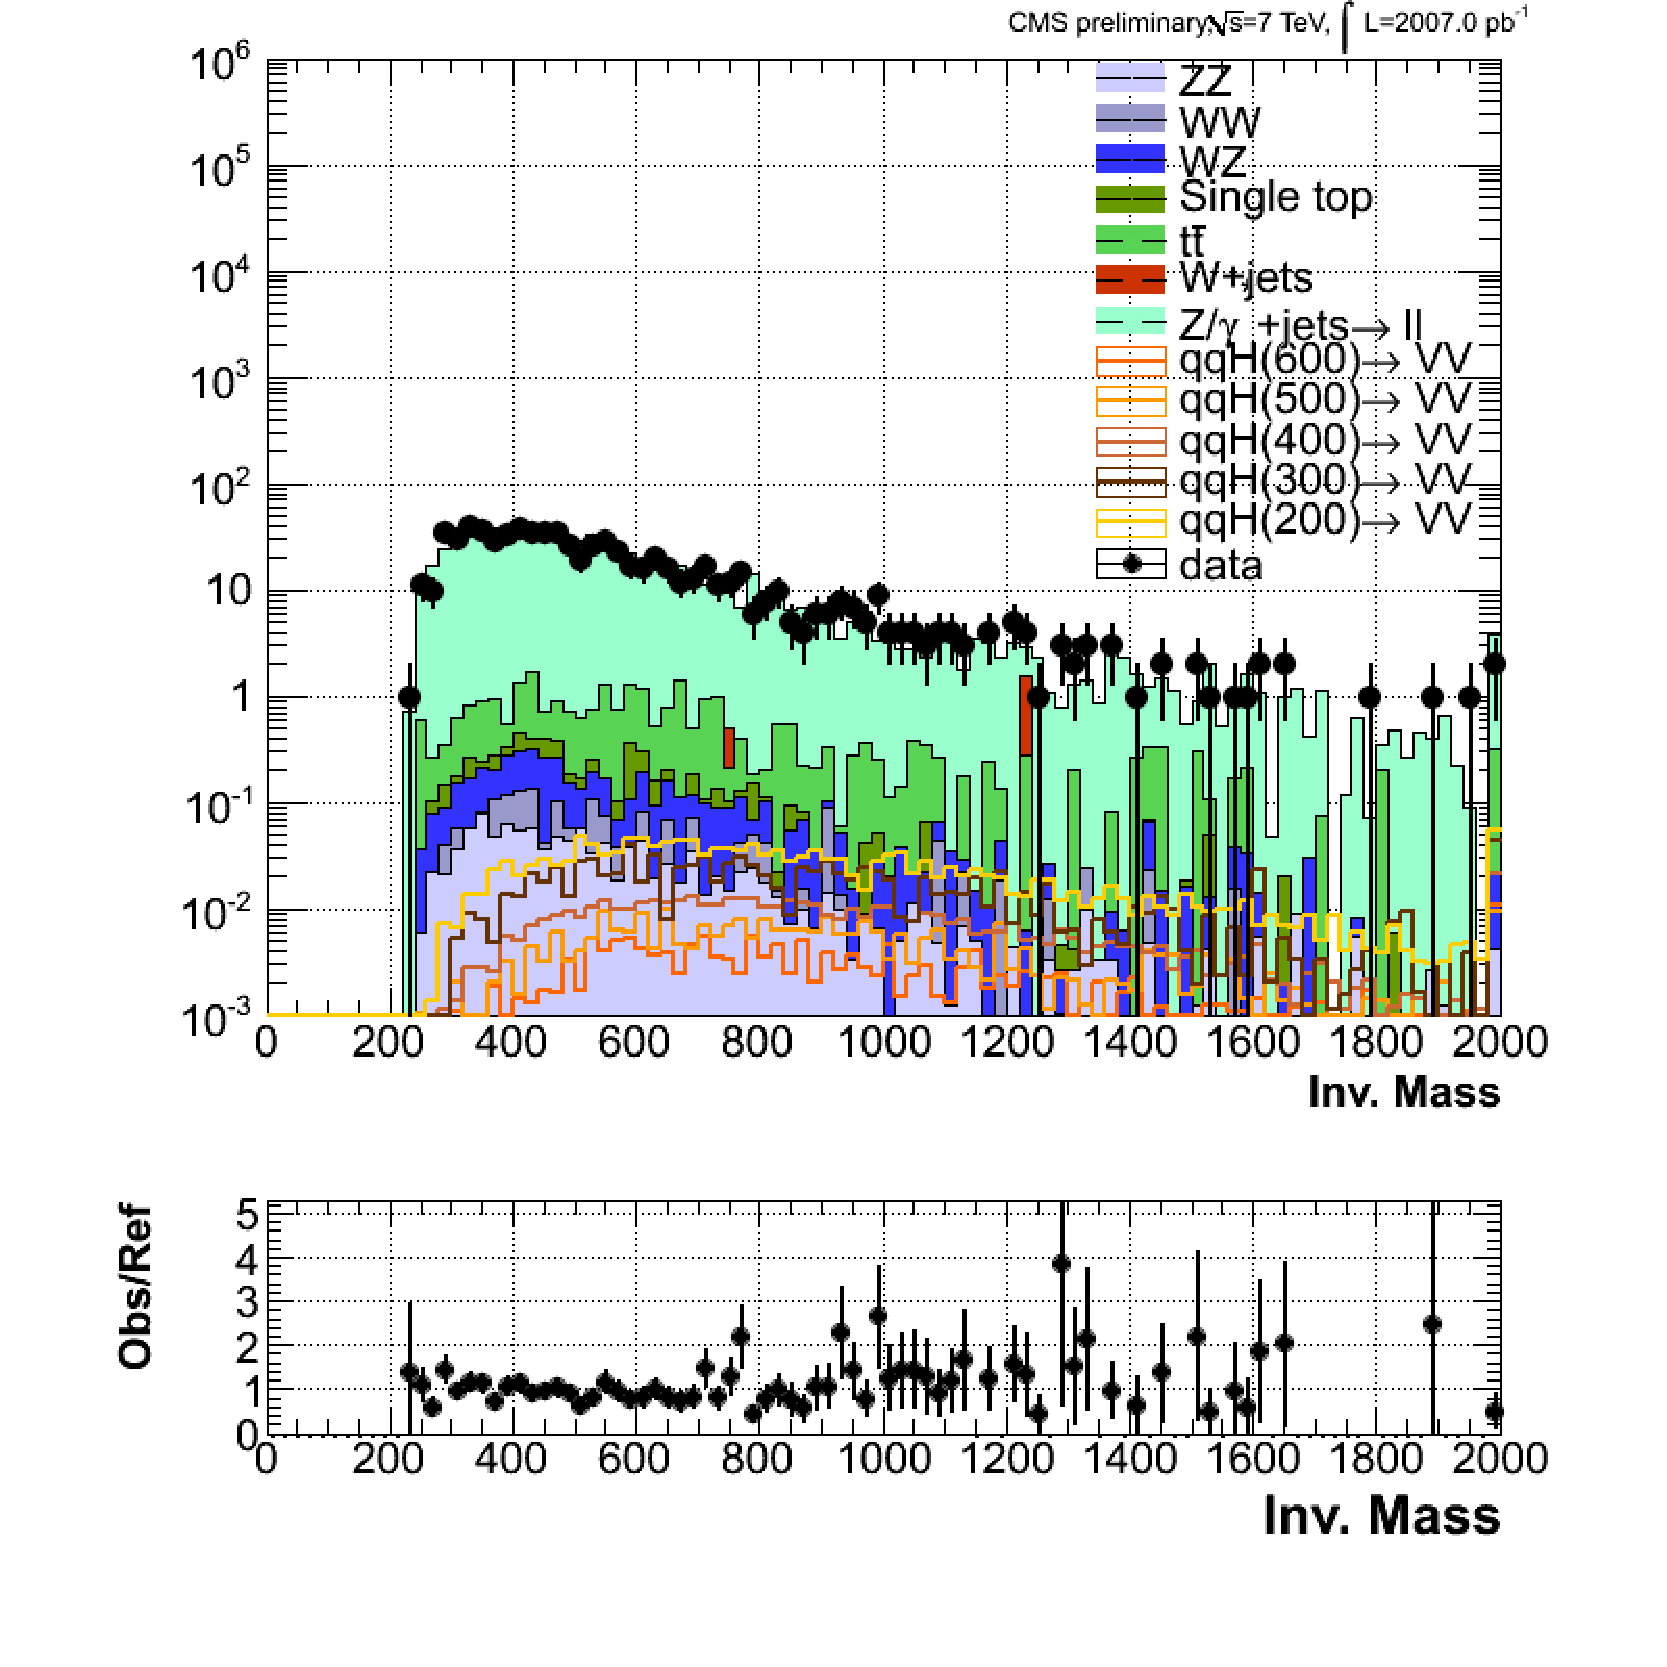
\includegraphics[width=0.46\textwidth]{img/ee_VBFiMass}
\caption{Distribution of the te invariant mass between the two VBF jets in di-muon ({\em left}) and di-electron ({\em right}).  Note that signal is populated only with VBF produced Higgs.}
\label{fig:vbfiMass}
\end{center}
\end{figure}


\begin{figure}[htp]
\begin{center}
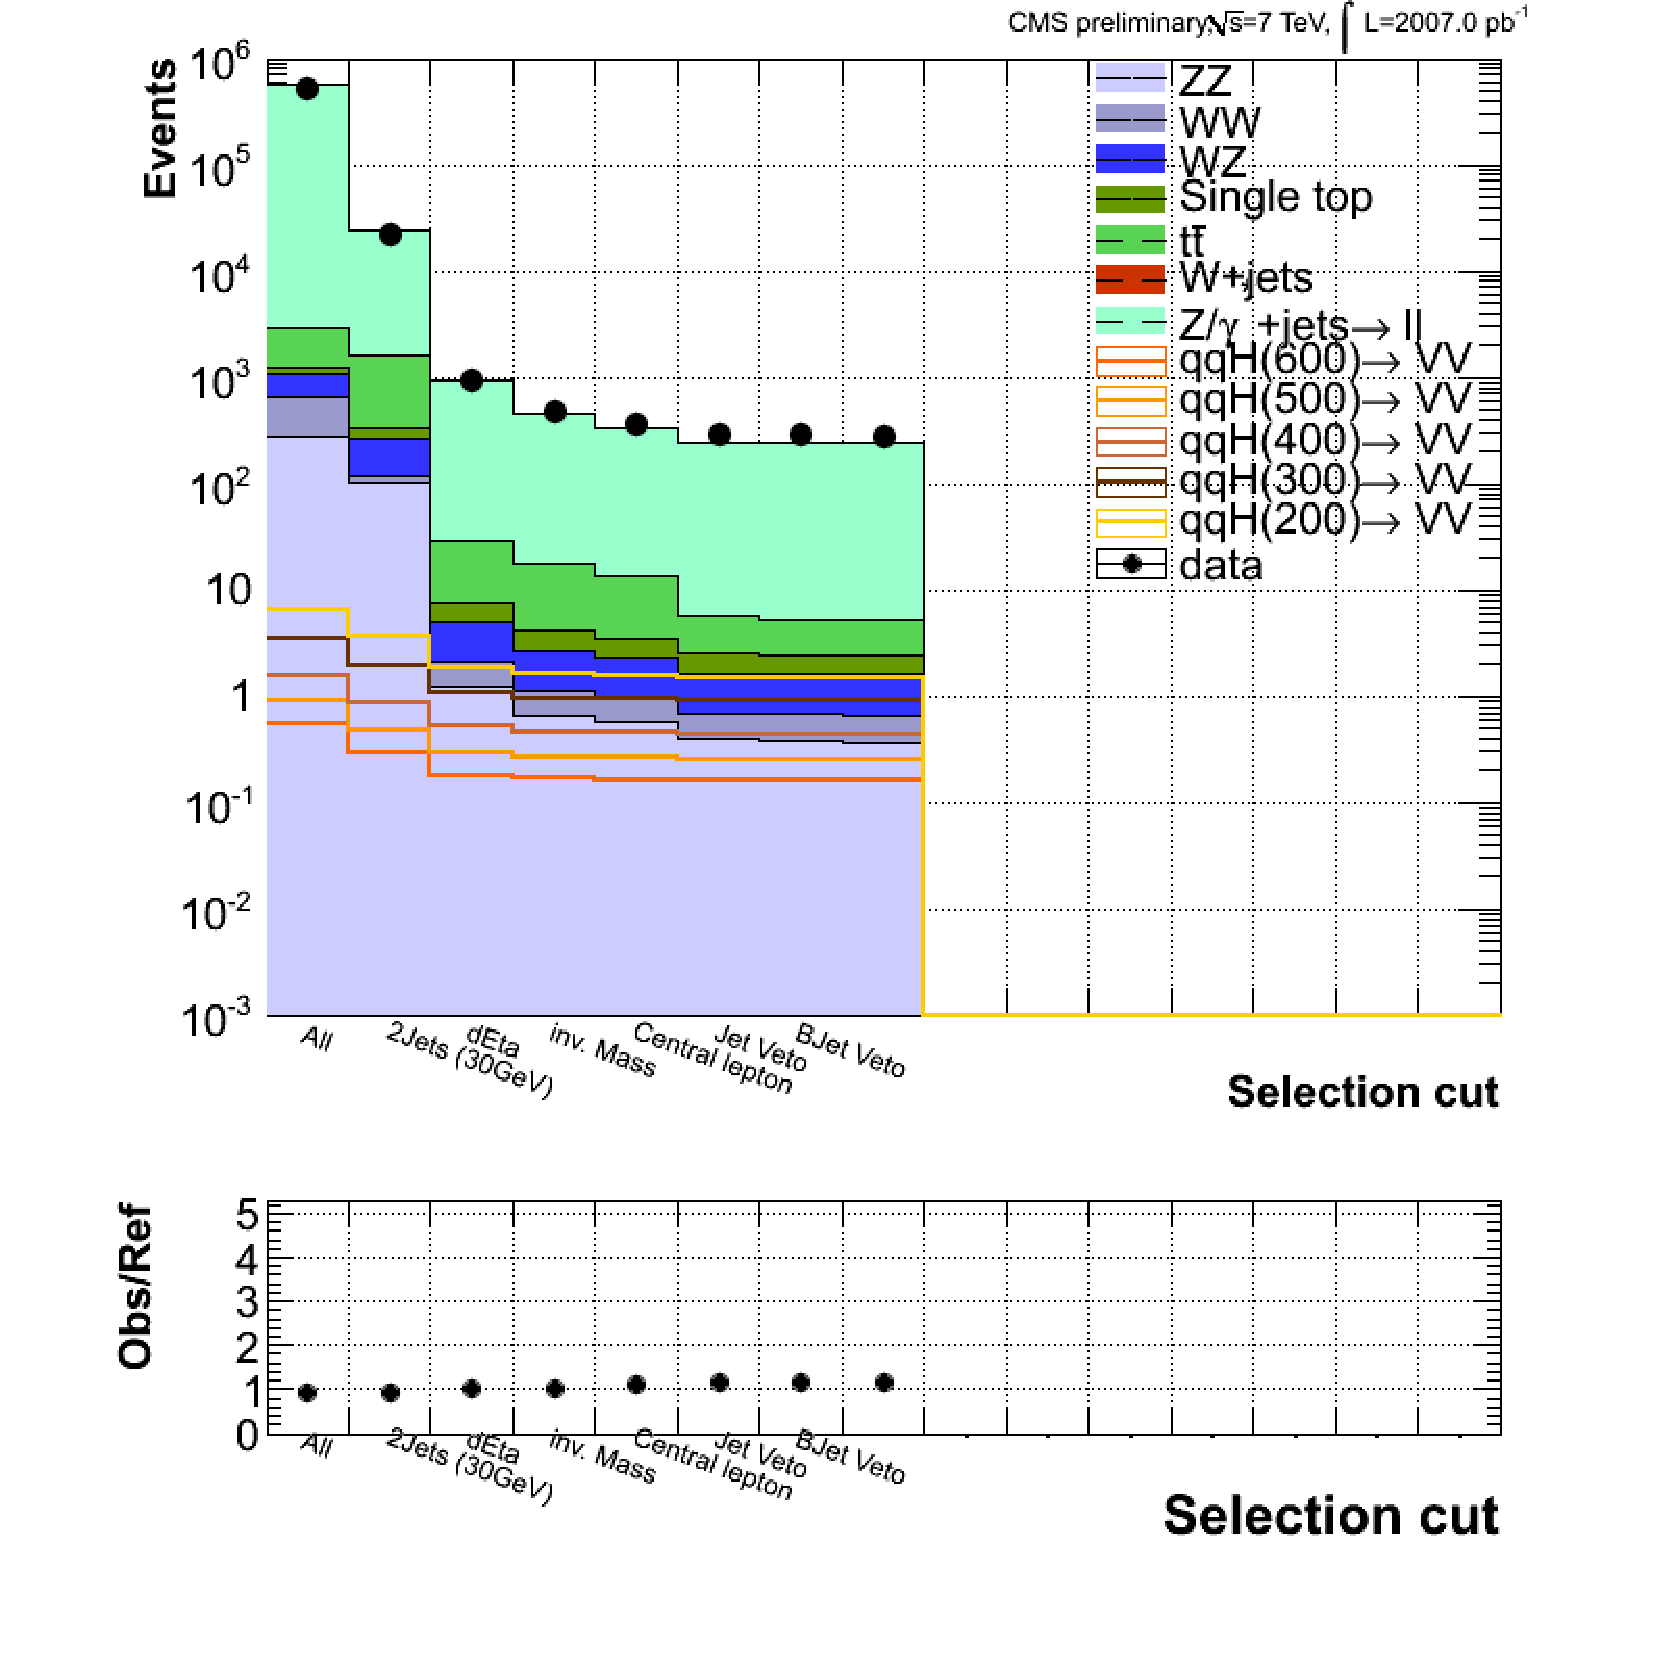
\includegraphics[width=0.46\textwidth]{img/mumu_VBFeventflowInc}
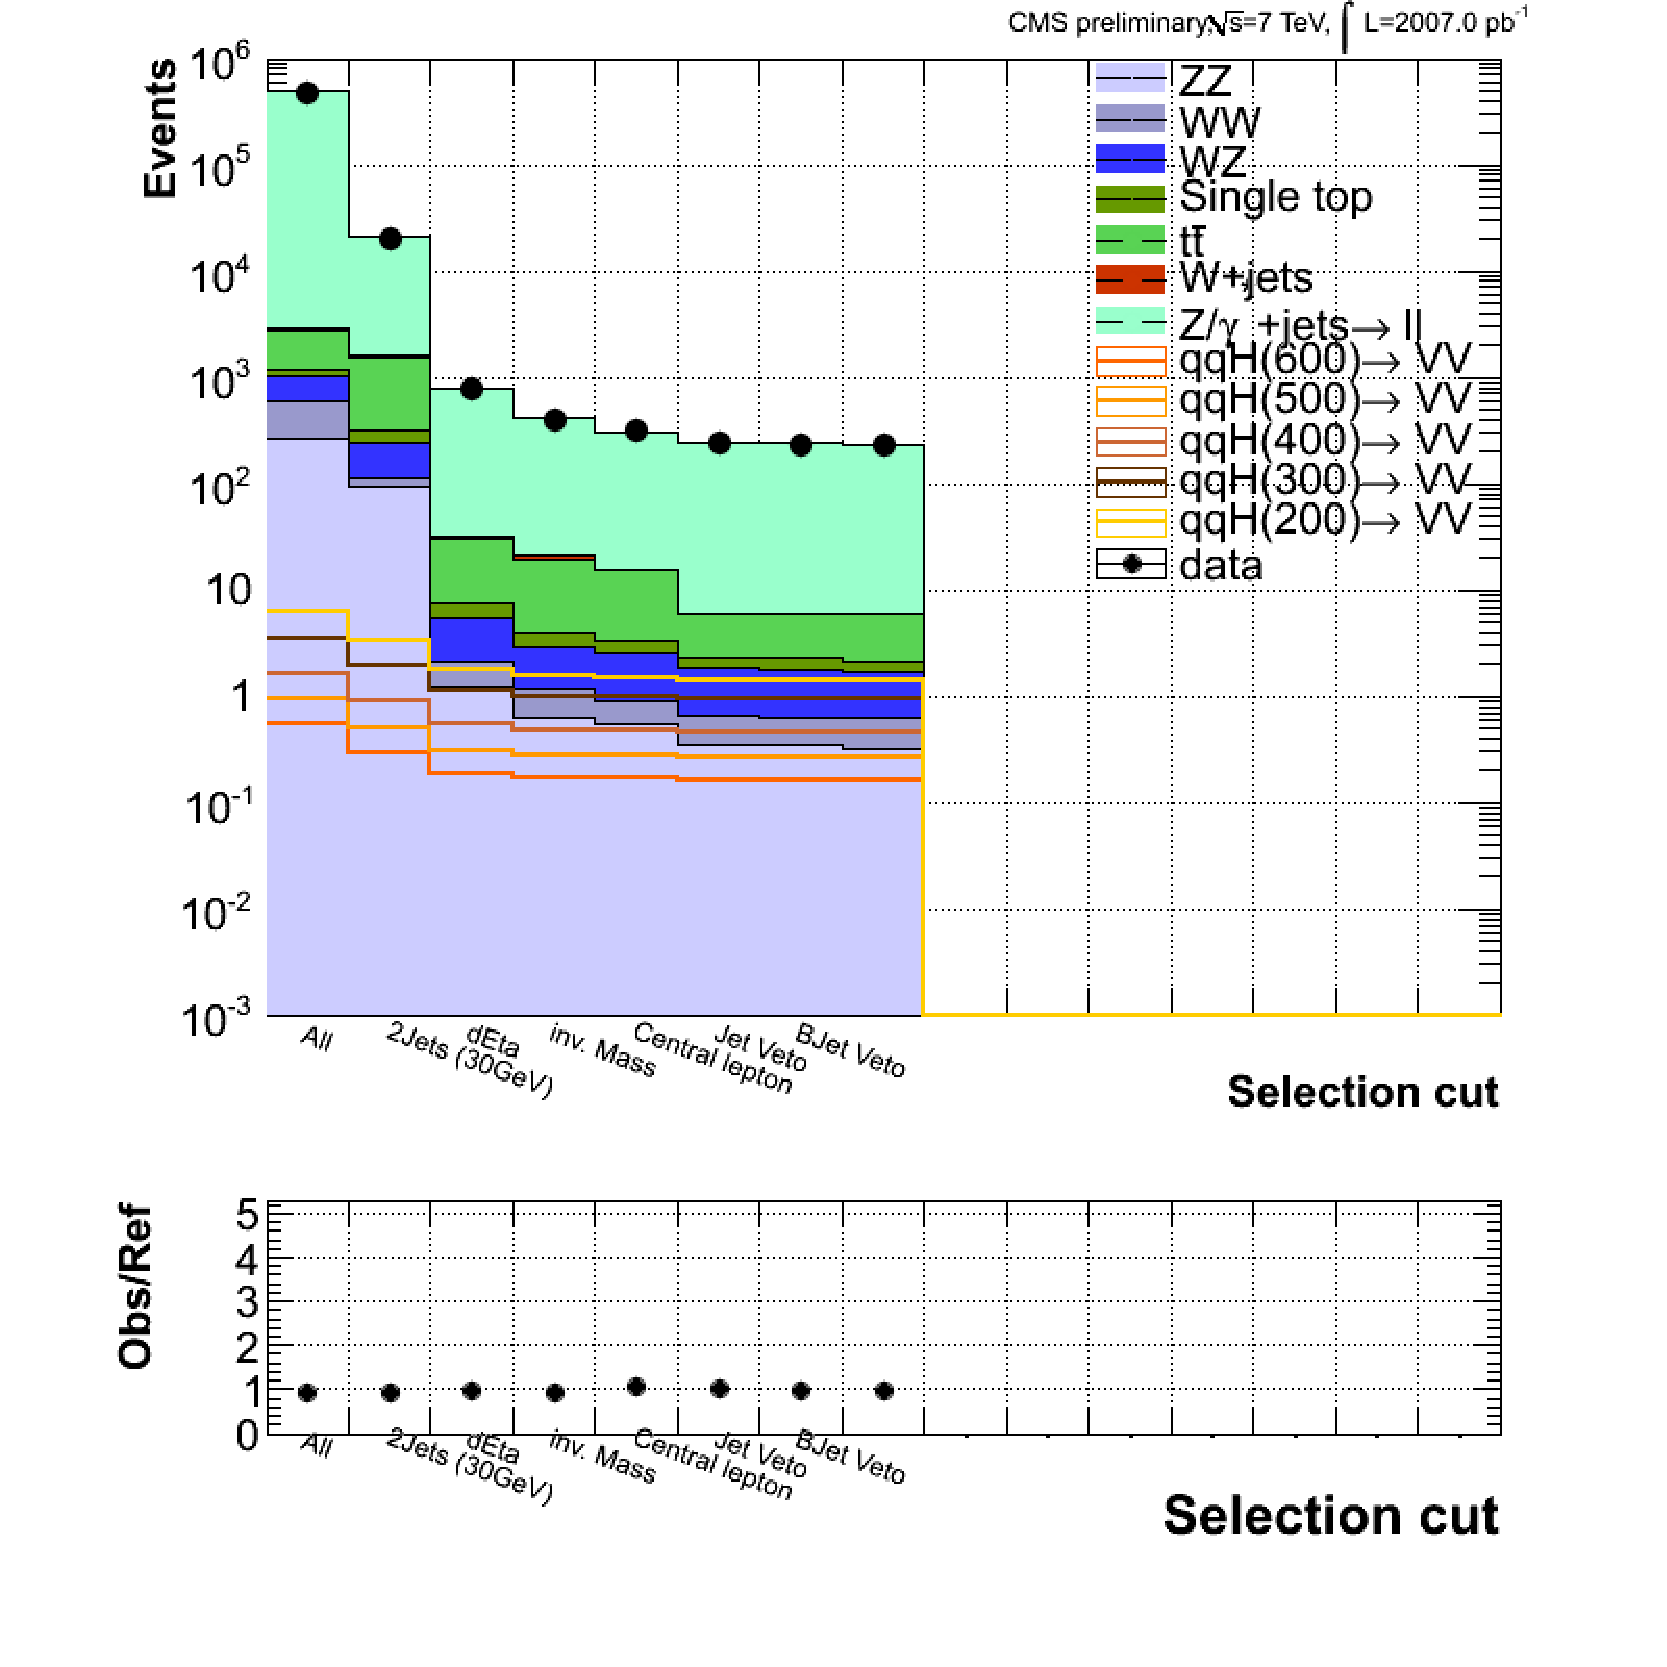
\includegraphics[width=0.46\textwidth]{img/ee_VBFeventflowInc}
\caption{Event flow for the VBF selection  in di-muon ({\em left}) and di-electron ({\em right}).  Note that signal is populated only with VBF produced Higgs.}
\label{fig:vbfeventflow}
\end{center}
\end{figure}

%%% MET
\item[Missing transverse energy] particle flow based \MET is used. The \MET is built from the vectorial sum of the transverse momentum all particle flow reconstructed candidates.
The verification of the reconstruction of the missing transverse energy will be the subject of a detailed discussion in Sec.~\ref{sec:met}
and a specific \MET based selection will be proposed to reduce more efficienctly the contamination from $Z$ events with minimal contamination from pileup.
Fig.~\ref{fig:metcontrol} shows the control distribution for the \MET after the $b$-jet veto has been applied. 
A wider resolution is observed in data with respect to the \MC prediction reinforcing the need to develop a detailed verification of its reconstruction
and a data-driven method to model the expected performance to remove $Z$ events.

\begin{figure}[htp]
\begin{center}
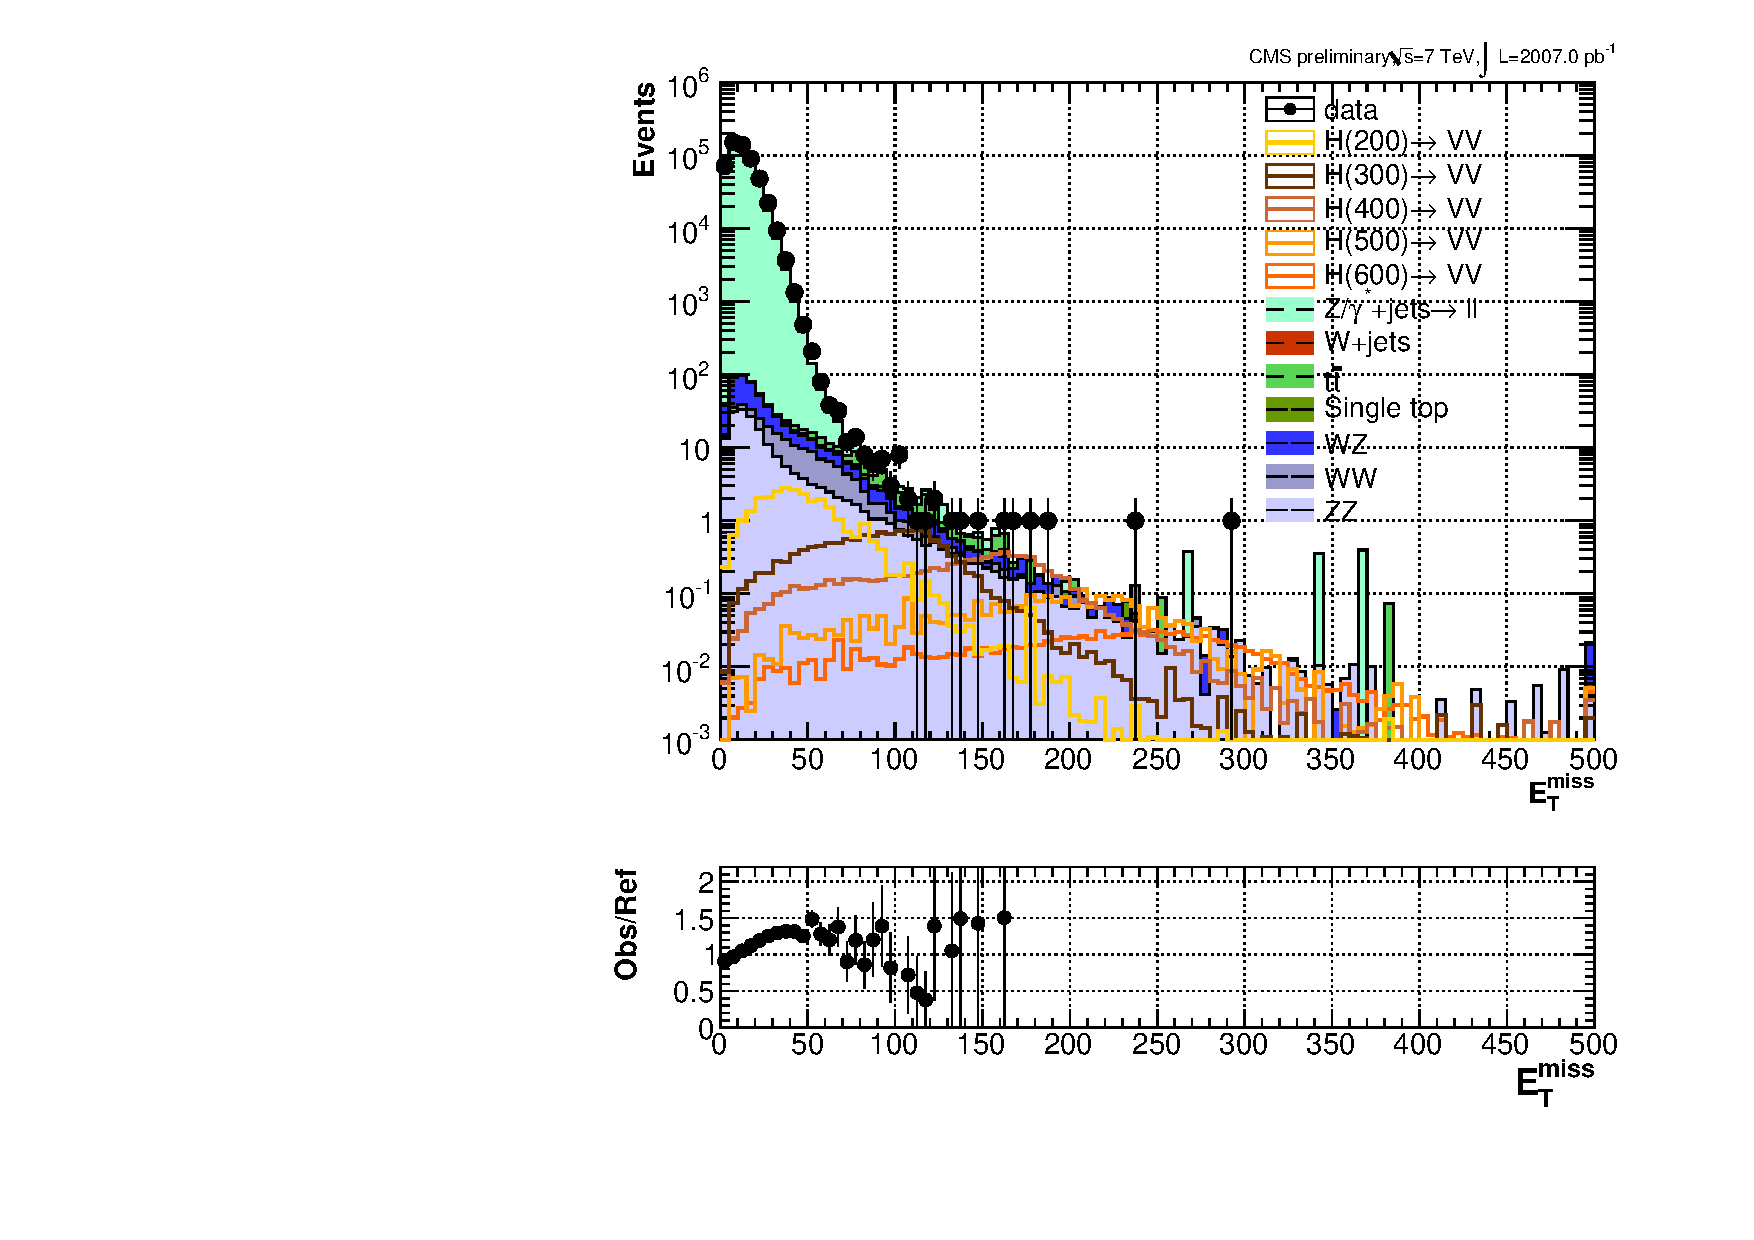
\includegraphics[width=0.46\textwidth]{img/mumu_met}
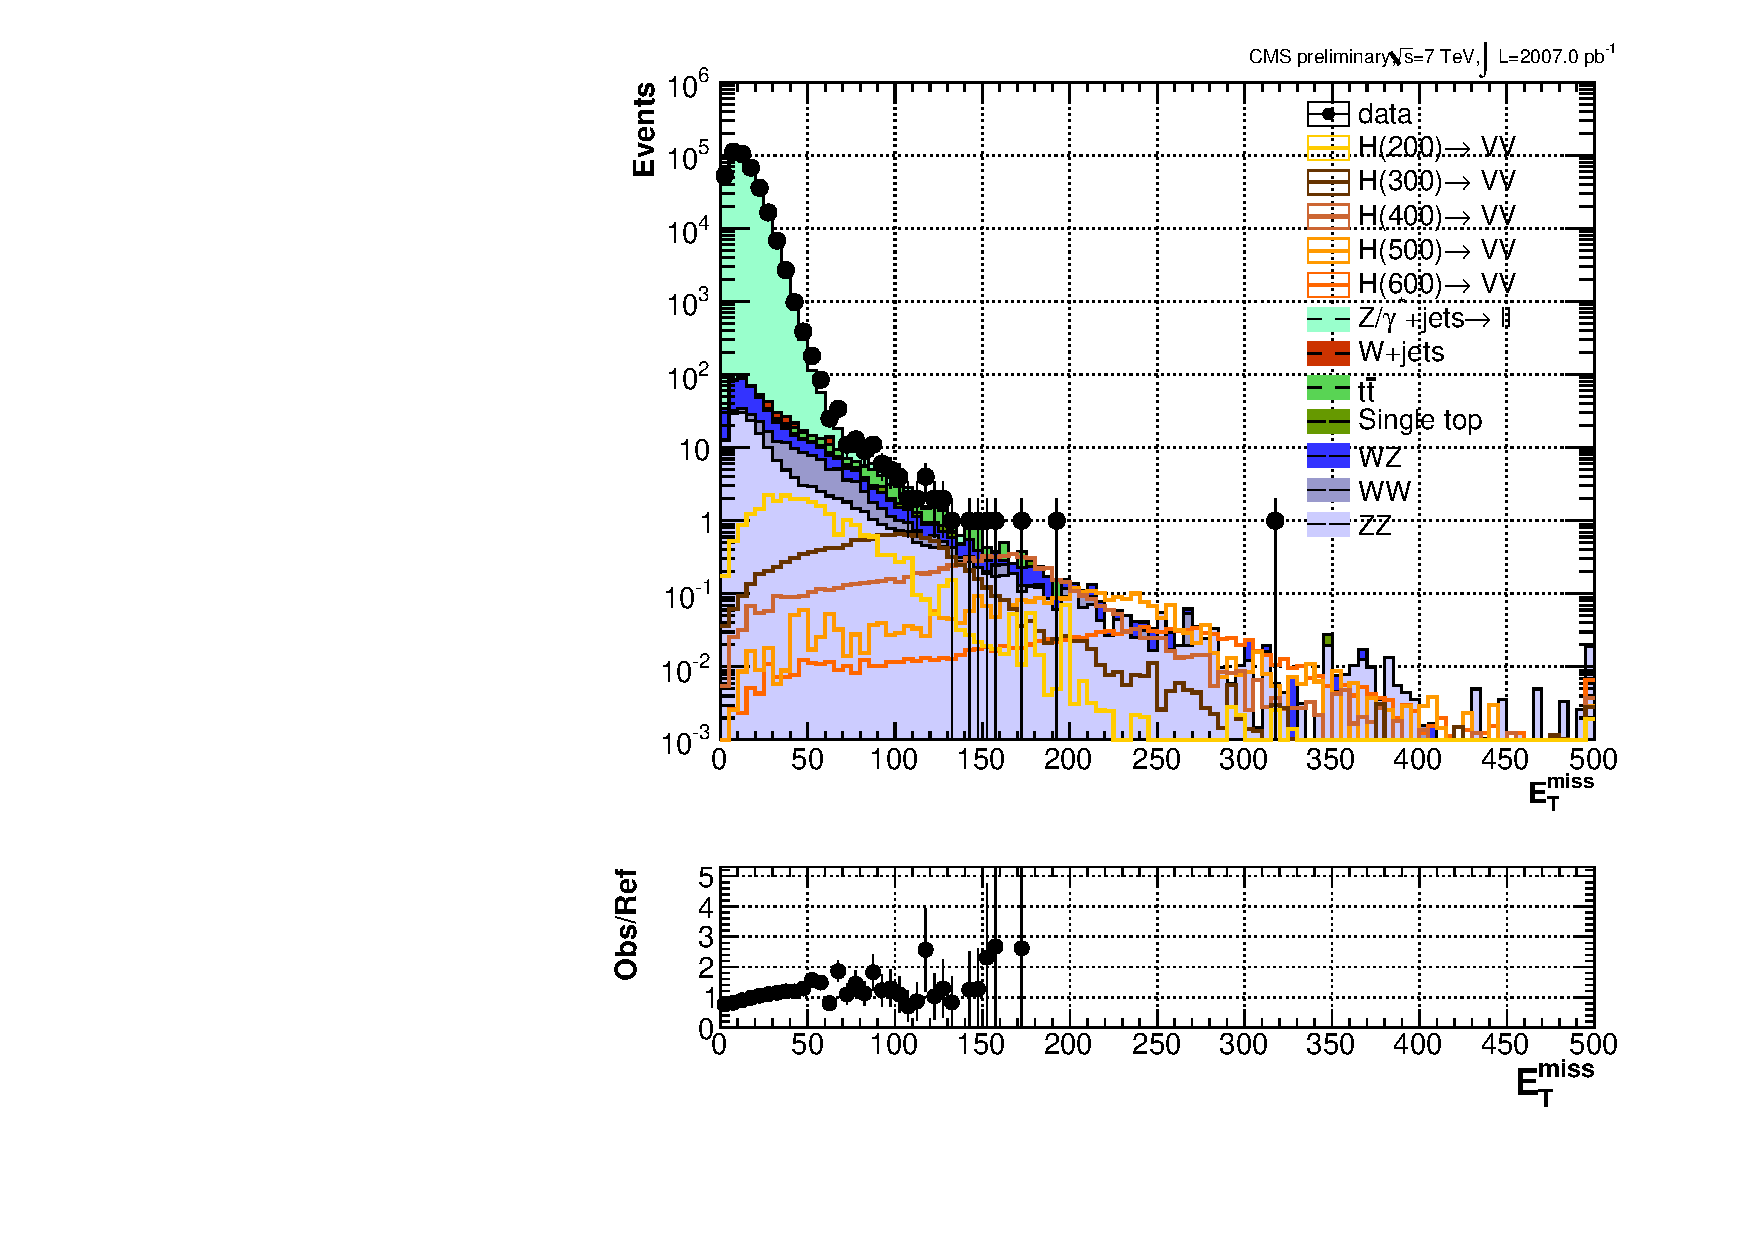
\includegraphics[width=0.46\textwidth]{img/ee_met}
\caption{\MET reconstructed in di-muon ({\em left}) and di-electron ({\em right}).}
\label{fig:metcontrol}
\end{center}
\end{figure}


\end{description}

In the next section the event yields after pre-selection of the dilepton sample are presented and discussed.


%%
%% EVENT YIELDS
%%
\subsection{Event yields after pre-seletion}
\label{subsec:eventyields}

The event yields after applying the pre-selection discussed in the previous section are shown in Table~\ref{tab:gluglupresamplecutflow}
for the  inclusive sample and in Table~\ref{tab:vbfpresamplecutflow} for the events tagged as VBF.
An overall difference of $<$4\% is observed in both $ee$ and $\mu\mu$ channels for the different event categories.
The pre-selected sample after the b-tagging veto (for the inclusive production)
or after the lepton+central jet veto (for the VBF category) are used as the starting point for the search for the Higgs boson.

%%%
\begin{table}[htp]
\caption{Event yields for a total integrated luminosity of 2007~pb$^{-1}$. The uncertainties quoted are statistical only.}
\label{tab:gluglupresamplecutflow}
\begin{center}
\begin{tabular}{lccc} \hline\hline
Selection                          & $|M-M_Z|<$15~GeV/c$^2$ & 3$^{rd}$-lepton veto & no b-tags\\ \hline
& & & \\\hline
\multicolumn{4}{c}{\bf $\mu\mu$ channel} \\\hline
H(200)$\rightarrow$ VV              & $ 31.2 \pm0.8 $  & $ 31.2 \pm0.8 $  & $ 28.6 \pm0.7 $  \\
H(300)$\rightarrow$ VV              & $ 14.47 \pm0.14 $  & $ 14.45 \pm0.14 $  & $ 13.21 \pm0.13 $  \\
H(400)$\rightarrow$ VV              & $ 8.94 \pm0.08 $  & $ 8.93 \pm0.08 $  & $ 8.04 \pm0.08 $  \\
H(500)$\rightarrow$ VV              & $ 3.21 \pm0.11 $  & $ 3.21 \pm0.11 $  & $ 2.86 \pm0.11 $  \\
H(600)$\rightarrow$ VV              & $ 1.383 \pm0.018 $  & $ 1.380 \pm0.018 $  & $ 1.220 \pm0.017 $  \\\hline
ZZ                                  & $ 244.0 \pm1.0 $  & $ 234.4 \pm1.0 $  & $ 180.9 \pm0.9 $  \\
WW                                  & $ 87.8 \pm1.6 $  & $ 87.7 \pm1.6 $  & $ 84.9 \pm1.6 $  \\
WZ                                  & $ 366.3 \pm2.1 $  & $ 330.0 \pm2.0 $  & $ 278.8 \pm1.8 $  \\
Single top                          & $ 35.1 \pm1.1 $  & $ 34.4 \pm1.0 $  & $ 10.1 \pm0.6 $  \\
$t\bar{t}$                          & $ 396 \pm8 $  & $ 389 \pm8 $  & $ 41.8 \pm2.5 $  \\
W+jets                              & $ 0.31 \pm0.31 $  & $ 0.31 \pm0.31 $  & $ 0.31 \pm0.31 $  \\
Z/$\gamma^{*}$+jets$\rightarrow$ ll & $ ( 532.4 \pm0.4 ) \times10^{3} $  & $ ( 531.8 \pm0.4 ) \times10^{3} $  & $ ( 519.3 \pm0.4 ) \times10^{3} $\\\hline
Total simulated                     & $ ( 533.5 \pm0.4 ) \times10^{3} $  & $ ( 532.9 \pm0.4 ) \times10^{3} $  & $ ( 519.9 \pm0.4 ) \times10^{3} $\\\hline
Data                                & $  553.8 \times10^{3} $            & $  553.0 \times10^{3} $  & $ 538.2 \times10^{3} $ \\\hline
& & & \\\hline
\multicolumn{4}{c}{\bf $ee$ channel} \\\hline
H(200)$\rightarrow$ VV & $ 29.6 \pm0.8 $  & $ 29.6 \pm0.8 $  & $ 27.0 \pm0.7 $  \\
H(300)$\rightarrow$ VV & $ 14.04 \pm0.13 $  & $ 14.01 \pm0.13 $  & $ 12.81 \pm0.13 $  \\
H(400)$\rightarrow$ VV & $ 9.04 \pm0.08 $  & $ 9.02 \pm0.08 $  & $ 8.09 \pm0.08 $  \\
H(500)$\rightarrow$ VV & $ 3.55 \pm0.11 $  & $ 3.53 \pm0.11 $  & $ 3.15 \pm0.11 $  \\
H(600)$\rightarrow$ VV & $ 1.464 \pm0.016 $  & $ 1.462 \pm0.016 $  & $ 1.281 \pm0.015 $  \\\hline
ZZ & $ 229.8 \pm1.0 $  & $ 213.1 \pm0.9 $  & $ 164.1 \pm0.8 $  \\
WW & $ 77.4 \pm1.5 $  & $ 77.3 \pm1.5 $  & $ 75.0 \pm1.5 $  \\
WZ & $ 360.4 \pm2.1 $  & $ 304.9 \pm1.9 $  & $ 256.4 \pm1.8 $  \\
Single top & $ 35.3 \pm1.1 $  & $ 34.6 \pm1.0 $  & $ 10.6 \pm0.6 $  \\
$t\bar{t}$   & $ 372 \pm7 $  & $ 365 \pm7 $  & $ 39.7 \pm2.4 $  \\
W+jets     & $ 39 \pm7 $  & $ 39 \pm7 $  & $ 37 \pm7 $  \\
Z/$\gamma^{*}$+jets$\rightarrow$ ll & $ ( 468.0 \pm0.4 ) \times10^{3} $  & $ ( 467.5 \pm0.4 ) \times10^{3} $  & $ ( 456.0 \pm0.4 ) \times10^{3} $ \\\hline
Total simulated & $ ( 469.2 \pm0.4 ) \times10^{3} $  & $ ( 468.5 \pm0.4 ) \times10^{3} $  & $ ( 456.6 \pm0.4 ) \times10^{3} $ \\\hline
data & $  473.8 \times10^{3} $  & $ 473.0 \times10^{3} $  & $  460.1 \times10^{3} $  \\\hline\hline
\end{tabular}
\end{center}
\end{table}

%%%
\begin{table}[htp]
\begin{center}
\caption{Incremental event yields for the VBF events selection.}
\label{tab:vbfpresamplecutflow}
\begin{tabular}{lccccc} \hline\hline
\multirow{2}{*}{Selection}  & $|M-M_Z|<$15~GeV/c$^2$    & \multirow{2}{*}{$\Delta\eta$} & \multirow{2}{*}{inv. Mass} & \multirow{2}{*}{Lep.+Jet Veto} \\
                            & + 2 jets ($p_T>30~GeV/c$) &                               &                            &                                \\ \hline
                         &  &  & &  & \\ \hline
                         & \multicolumn{4}{c}{\bf $\mu\mu$ channel} \\\hline
qqH(200)$\rightarrow$ VV & $ 3.57 \pm 0.04 $  & $ 1.867 \pm 0.032 $  & $ 1.597 \pm 0.030 $  & $ 1.466 \pm 0.028 $   \\
qqH(300)$\rightarrow$ VV & $ 1.93 \pm 0.06 $  & $ 1.09 \pm 0.05 $  & $ 0.95 \pm 0.04 $   & $ 0.90 \pm 0.04 $   \\
qqH(400)$\rightarrow$ VV & $ 0.848 \pm 0.010 $  & $ 0.518 \pm 0.008 $  & $ 0.467 \pm 0.007 $   & $ 0.434 \pm 0.007 $   \\
qqH(500)$\rightarrow$ VV & $ 0.480 \pm 0.016 $  & $ 0.296 \pm 0.012 $  & $ 0.268 \pm 0.012 $   & $ 0.254 \pm 0.011 $   \\
qqH(600)$\rightarrow$ VV & $ 0.285 \pm 0.010 $  & $ 0.181 \pm 0.008 $  & $ 0.169 \pm 0.008 $   & $ 0.158 \pm 0.008 $   \\
\hline
ZZ & $ 102.1 \pm 0.6 $  & $ 1.25 \pm 0.07 $  & $ 0.65 \pm 0.05 $   & $ 0.39 \pm 0.04 $   \\
WW & $ 16.2 \pm 0.7 $  & $ 0.89 \pm 0.16 $  & $ 0.50 \pm 0.12 $   & $ 0.30 \pm 0.09 $   \\
WZ & $ 142.0 \pm 1.3 $  & $ 2.87 \pm 0.18 $  & $ 1.57 \pm 0.13 $  & $ 0.96 \pm 0.10 $   \\
Single top & $ 69.9 \pm 1.5 $  & $ 2.60 \pm 0.30 $  & $ 1.47 \pm 0.23 $   & $ 0.82 \pm 0.17 $   \\
$t\bar{t}$ & $ 1302 \pm 14 $  & $ 20.8 \pm 1.7 $  & $ 13.6 \pm 1.4 $   & $ 2.9 \pm 0.6 $   \\
W+jets & $ 1.9 \pm 1.9 $   &  & &    \\
Z/$\gamma^{*}$+jets$\rightarrow$ ll & $ ( 22.08 \pm 0.08 ) \times10^{3} $  & $ 902 \pm 16 $  & $ 444 \pm 11 $   & $ 240 \pm 8 $   \\
Total expected & $ ( 23.71 \pm 0.08 ) \times10^{3} $  & $ 931 \pm 16 $  & $ 462 \pm 11 $   & $ 245 \pm 8 $  \\
\hline
data & $ ( 21.63 \pm 0.15 ) \times10^{3} $  & $ 940 \pm 31 $  & $ 466 \pm 22 $   & $ 285 \pm 17 $   \\
\hline
                         &  &  & &  & \\ \hline
 & \multicolumn{4}{c}{\bf $ee$ channel} \\\hline
qqH(200)$\rightarrow$ VV & $ 3.36 \pm 0.04 $  & $ 1.735 \pm 0.031 $  & $ 1.512 \pm 0.029 $   & $ 1.402 \pm 0.028 $   \\
qqH(300)$\rightarrow$ VV & $ 1.95 \pm 0.06 $  & $ 1.13 \pm 0.05 $  & $ 1.00 \pm 0.04 $   & $ 0.93 \pm 0.04 $   \\
qqH(400)$\rightarrow$ VV & $ 0.885 \pm 0.010 $  & $ 0.537 \pm 0.008 $  & $ 0.482 \pm 0.007 $   & $ 0.448 \pm 0.007 $   \\
qqH(500)$\rightarrow$ VV & $ 0.491 \pm 0.016 $  & $ 0.309 \pm 0.013 $  & $ 0.280 \pm 0.012 $   & $ 0.263 \pm 0.012 $   \\
qqH(600)$\rightarrow$ VV & $ 0.290 \pm 0.010 $  & $ 0.186 \pm 0.008 $  & $ 0.172 \pm 0.008 $   & $ 0.160 \pm 0.008 $   \\
\hline
ZZ & $ 94.5 \pm 0.6 $  & $ 1.21 \pm 0.07 $  & $ 0.64 \pm 0.05 $  & $ 0.35 \pm 0.04 $   \\
WW & $ 17.1 \pm 0.7 $  & $ 0.90 \pm 0.16 $  & $ 0.53 \pm 0.12 $  & $ 0.29 \pm 0.09 $   \\
WZ & $ 133.8 \pm 1.3 $  & $ 3.37 \pm 0.20 $  & $ 1.79 \pm 0.14 $  & $ 1.17 \pm 0.12 $   \\
Single top & $ 66.7 \pm 1.5 $  & $ 1.95 \pm 0.24 $  & $ 1.08 \pm 0.18 $  & $ 0.47 \pm 0.11 $   \\
$t\bar{t}$ & $ 1254 \pm 14 $  & $ 22.7 \pm 1.8 $  & $ 15.7 \pm 1.5 $  & $ 3.7 \pm 0.7 $   \\
W+jets & $ 27 \pm 7 $  & $ 1.5 \pm 1.3 $  & $ 1.5 \pm 1.3 $   &    \\
Z/$\gamma^{*}$+jets$\rightarrow$ ll & $ ( 19.80 \pm 0.08 ) \times10^{3} $  & $ 766 \pm 15 $  & $ 391 \pm 11 $   & $ 231 \pm 8 $   \\
Total expected & $ ( 21.39 \pm 0.08 ) \times10^{3} $  & $ 798 \pm 15 $  & $ 413 \pm 11 $   & $ 237 \pm 8 $   \\
\hline
data & $ ( 19.86 \pm 0.14 ) \times10^{3} $  & $ 782 \pm 28 $  & $ 389 \pm 20 $   & $ 235 \pm 15 $ \\
\hline \hline
\end{tabular}
\end{center}
\end{table}


%%
%%
%%
\clearpage
\section{Verification of the reconstructed missing transverse energy}
\label{sec:met}

The following section we discuss different strategies adopted in the choice of the variable used to reduce the contamination
from the instrumental background, i.e., from processes in which the \MET is mismeasured.
The main sources of mis-measurement of this quantity are the underestimate of the hadronic recoil
of $Z$ bosons, due to jet energy scale and resolution as well as detector acceptance, and the contamination from pileup.
In Sec.~\ref{subsec:redmet} we describe a variable developed with the purpose of reducing the underestimation of the hadronic recoil of the $Z$ bosons.
The performance of this variable is compared with standard \MET among other \MET related variables.
In Sec.~\ref{subsec:fjpucontrol} we describe a strategy aimed to control pileup
in the high luminosity regime based on the clustering of energy oriented from the reconstructed vertices.
As this strategy is limited by the acceptance of the tracker (roughly up to $|\eta|<$2.4)
which corresponds also the acceptance region for the signal we argue further
that by comparing the components of the total \MET in the central and forward region of the detector
it is possible to discriminate further the instrumental background from processes which produce real \MET.

%%%
%%% REDUCED MET
%%%
\subsection{Description of the reduced \MET method}
\label{subsec:redmet}

We adopt the definition of reduced missing transverse energy (\RMET) for our analysis.
The definiton is an upgrade of the original concept developed by the D0 collaboration~\cite{Abazov:2008yf}.
In this method the recoil of the dilepton is decomposed using either the dilepton:

\begin{itemize}
\item direction, in case the two leptons are collimated, i.e. $\Delta\phi^{ll}<\pi/2$;
\item bisector, in case the two leptons are reconstructed with an open angle, i.e.   $\Delta\phi^{ll}>\pi/2$;
\end{itemize}

In the case of two leptons reconstructed with an open angle 
the bisector of the dilepton is defined transversely to the axis which maximizes the dilepton transverse momentum,  i.e. the thrust axis($\vec{t}$):

\begin{equation}
\vec{t} =\frac{1}{|\vec{l}_1-\vec{l}_2|}(\vec{l}_1 - \vec{l}_{2})
\label{eq:thrust} 
\end{equation}

where $l_1$ ($l_2$) is the 3-momentum of the leading (trailer) lepton. 
We adopt the convention to define the bisector ($\vec{b}$) as pointing in the same direction as the leading lepton, i.e.:

\begin{equation}
\vec{b}\cdot\vec{t}=0 ~~~\wedge~~~ \vec{b}\cdot\vec{l}_1>0
\label{eq:bisector} 
\end{equation}

Fig.~\ref{fig:dildecomposition} illustrates the decomposition of the transverse plane just described.
The procedure is expected to have optimal resolution on the lepton reconstruction
minimizing detector effects which may affect the dilepton $p_T$ momentum (i.e.$ p_T^{ll}$).
Even if these effects are expected to be small due to good reconstruction quality of muons and electrons in CMS
we have opted to follow this approach and refer to further details on the method 
to~\cite{Banfi:2010cf} and~\cite{Abazov:2010mk}.

\begin{figure}[htp]
\begin{center}
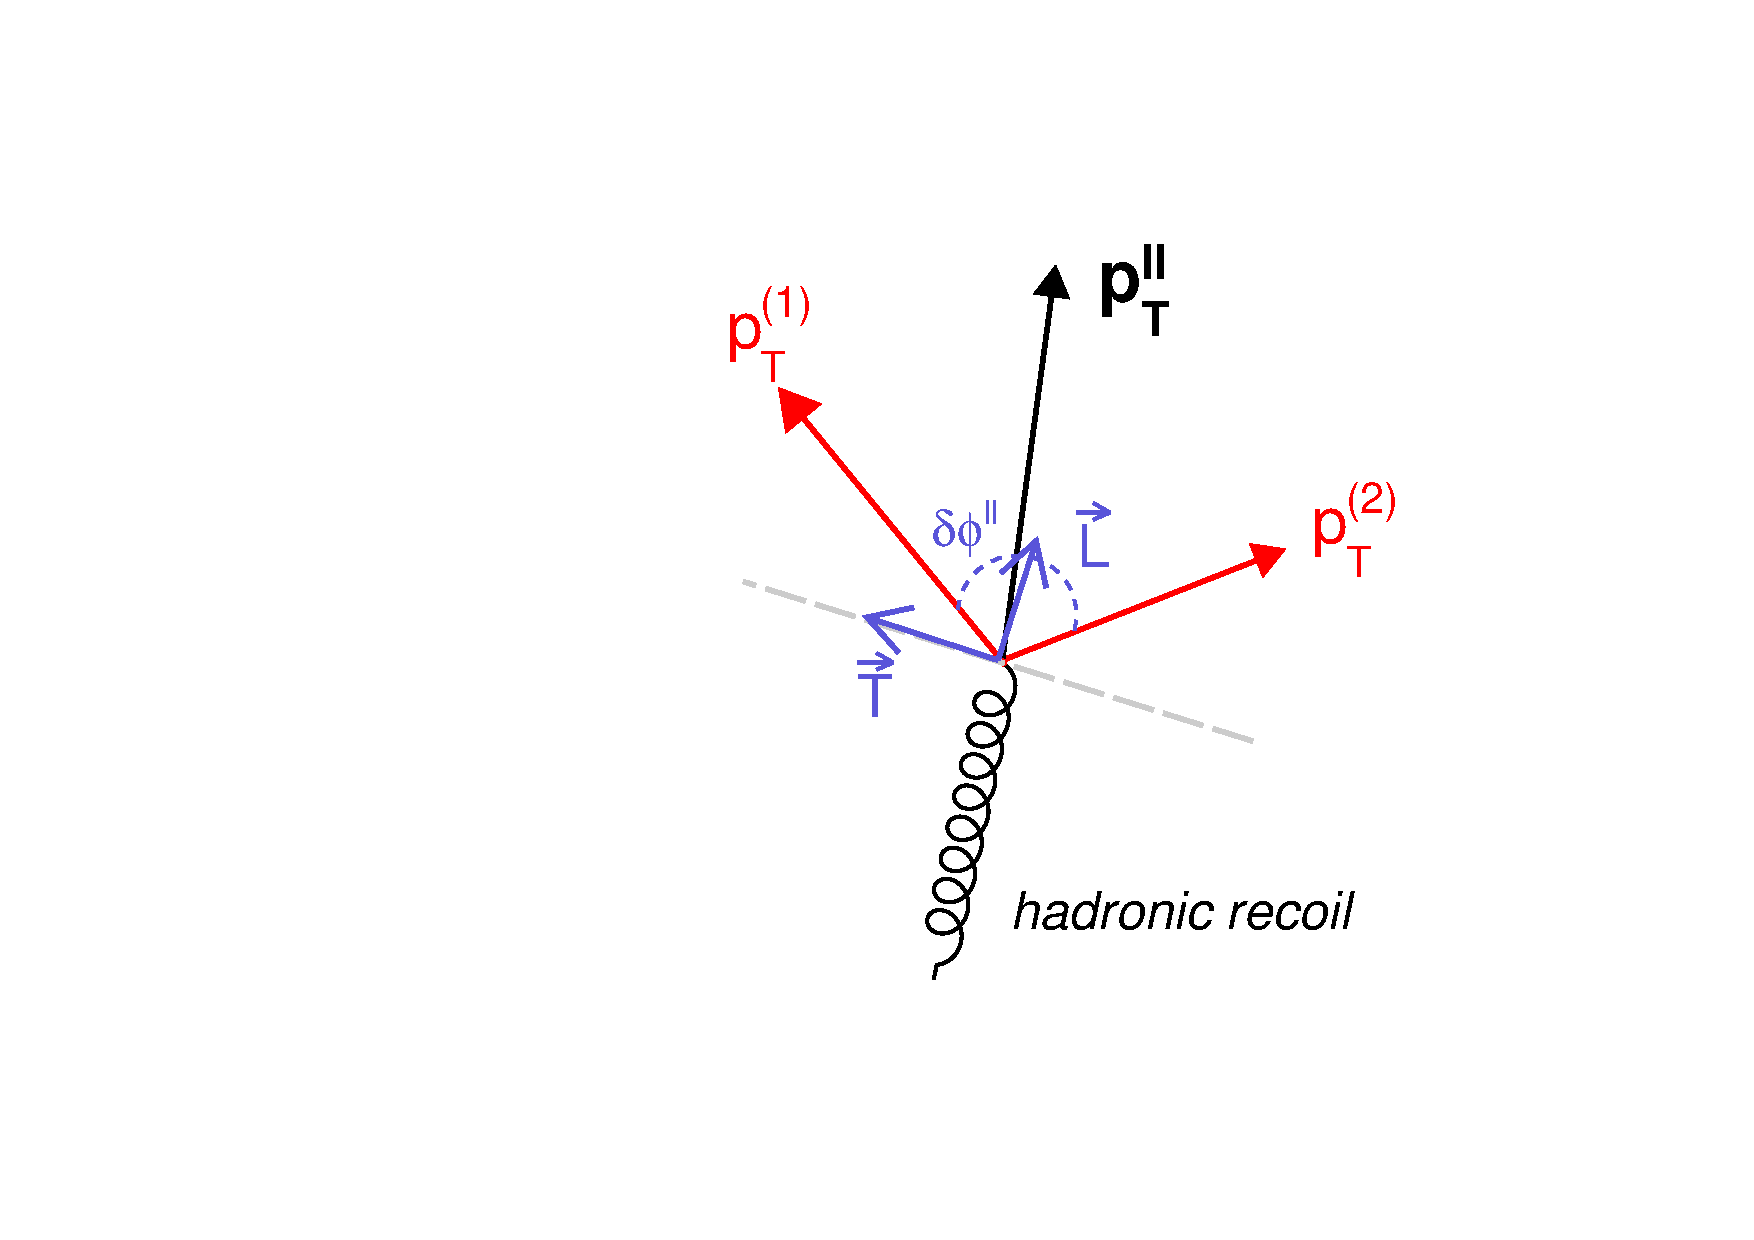
\includegraphics[width=0.6\textwidth]{img/dileptonDecomposition}
\caption{Illustration of the variables used to decompose the transverse plane based on the reconstructed dilepton kinematics.}
\label{fig:dildecomposition}
\end{center}
\end{figure}

The thrust and bisector are used to define the projections of the dilepton recoil which can be estimated from two sources:

\begin{itemize}
\item clustered recoil ($\vec{R}^{\text{clust}}$), from the jets reconstructed in the event;
\item unclustered recoil ($\vec{R}^{\text{uncl}}$), from the sum of all particle flow candidates with the exception of the two leptons;
\end{itemize}

Originally the \RMET variable is computed with the following prescriptions:

\begin{enumerate}
\item the jets which contribute to each component of $\vec{R}^{\text{clust}}$ have to be found in the opposite direction with respect to the correspondent dilepton projection  
\item likewise the projections of the unclustered recoil are considered to be 0 if pointing in the same direction as the correspondent dilepton projection
\item the estimate of the recoil along each direction is made conservatively by taking the minimum of the two estimate, i.e. $R_i = \min \{ R_i^{\text{clust}},R_i^{\text{uncl}} \}$ 
\end{enumerate}

In this study we argue that 1. and 2. should not be used as they lead to an incomplete description of the recoil of the dilepton system for both instrumental background
(i.e. $Z$ events) and signal events.
In the first case the prescription to use jets which point in the opposite direction of the dilepton is compromised by the ocurrence of jet production
in the underlying event or even by multiple interaction. If only a subset of the jets is accounted for this leads inevitably to a wrong estimate of the true recoil.
In the second case we argue that highly boosted Higgs will be measured with the two Z's in the same hemisphere and therefore both the dilepton and the \MET will be pointing in the same direction
and found to be recoiling against a jet system. For these topologies the recoil will be estimated as being 0, leading to a consequent inefficiency of identifying the signal at high values of \RMET.
Instead we define \RMET from the minimum imbalance found using either the clustered or the unclustered recoil of the system.
Each component of \RMET is computed and minimized individually as

\begin{equation}
{\rm red-}E_{T_i}^{miss,k} =\vec{p}_{T}^{ll}\cdot \vec{i} + \alpha R^{\text{k}}_{i}
\label{eq:rmet}
\end{equation}

where k=clustered/unclustered and $\alpha$ is a scale factor which we consider always to be 1.
The absolute \RMET measurement is taken from the quadratic sum of the two components.
The procedure just described assumes a conservative scenario for jet energy and unclustered \MET reconstruction and resolution.
It is also expected to be effective against pileup events as jets are seeded using particle flow candidates associated to the primary vertex selected for each event. 
Our definition of \RMET is compared with the original one from D0 in Fig.~\ref{fig:redmet} for di-muon events.
It can be seen that the D0 definition yields a distribution with a very good resolution but which artificially 
accumulates events with \RMET=0 even for the signal. This result is strictly related to the topology of the boosted Higgs events
and can be mostly identified from events with 1 or 2 jets.
It can also be observed a better agreement between data and \MC for the definition of \RMET adopted by us.

\begin{figure}[htp]
\begin{center}
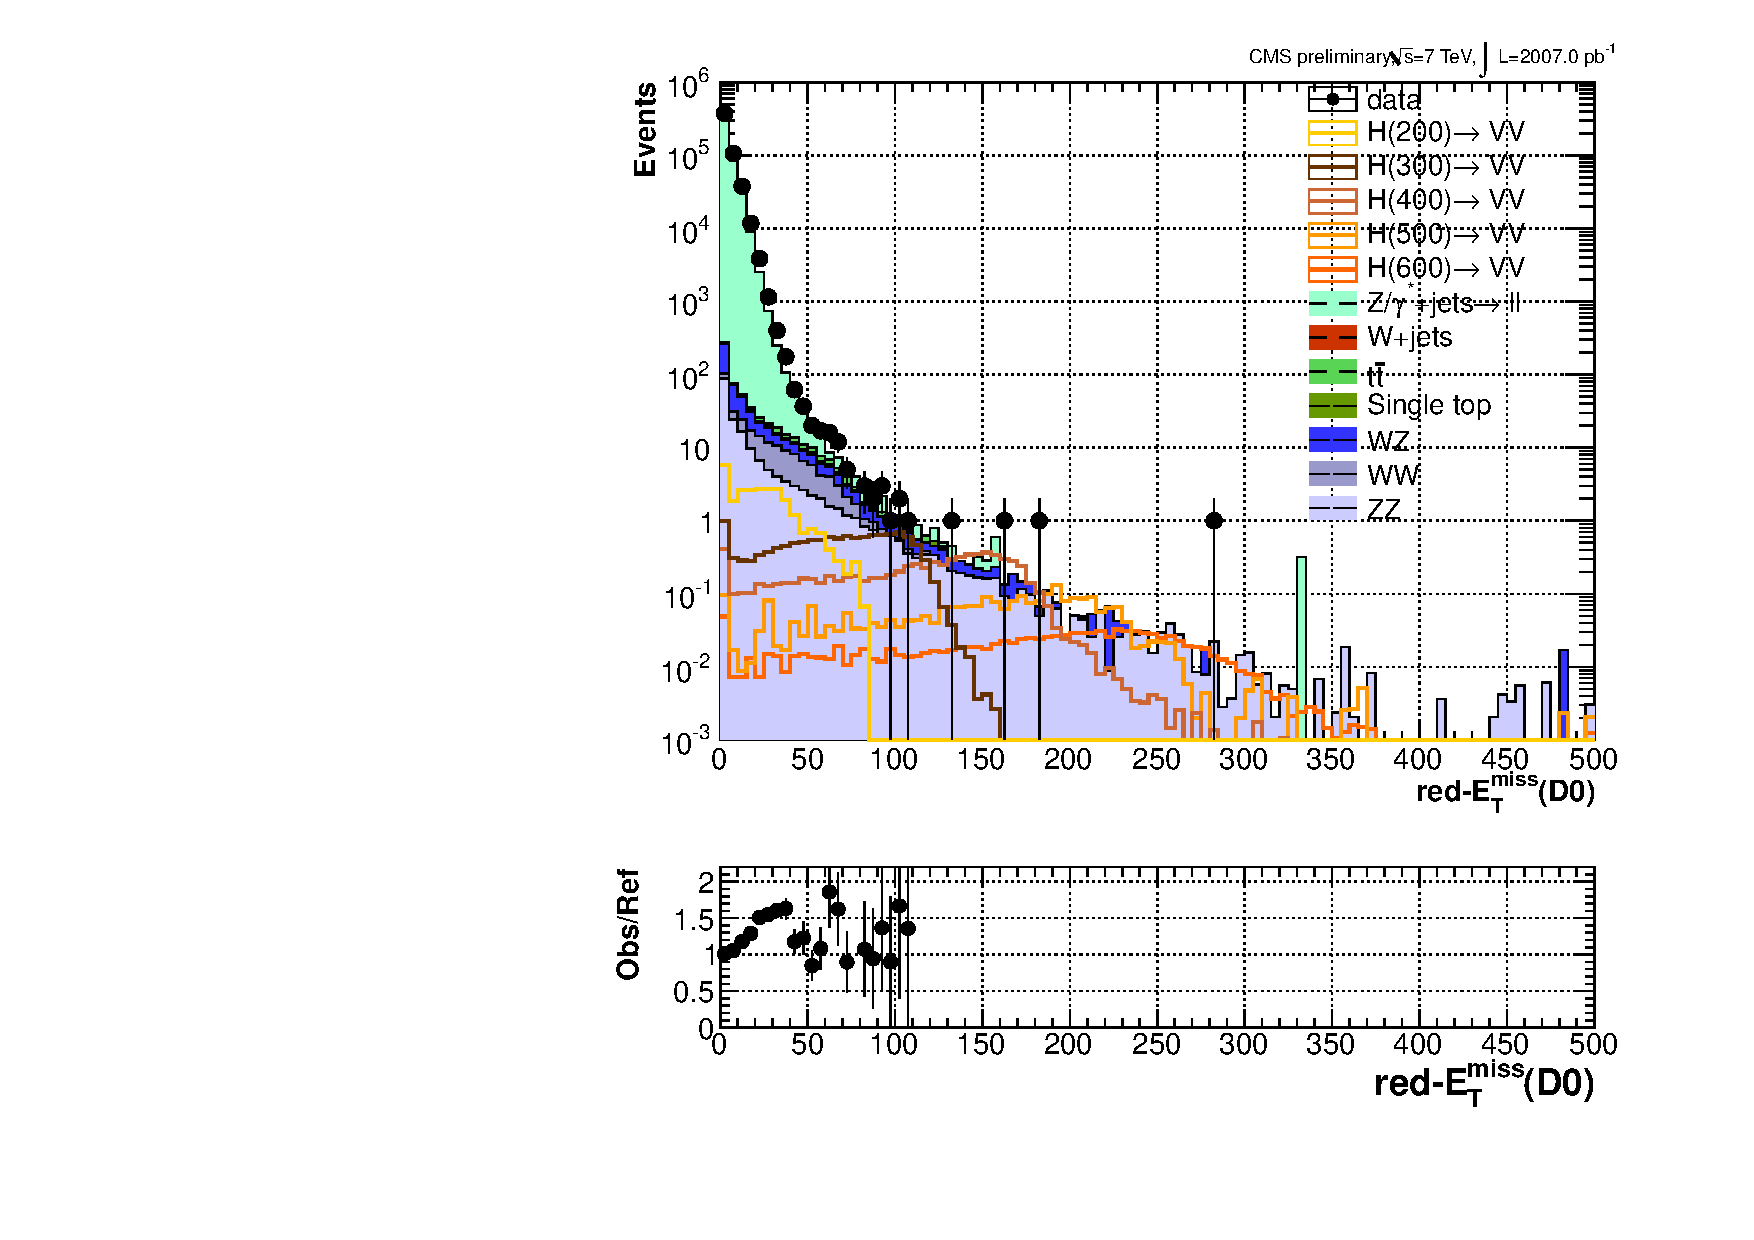
\includegraphics[width=0.45\textwidth]{img/mumu_redMetD0}
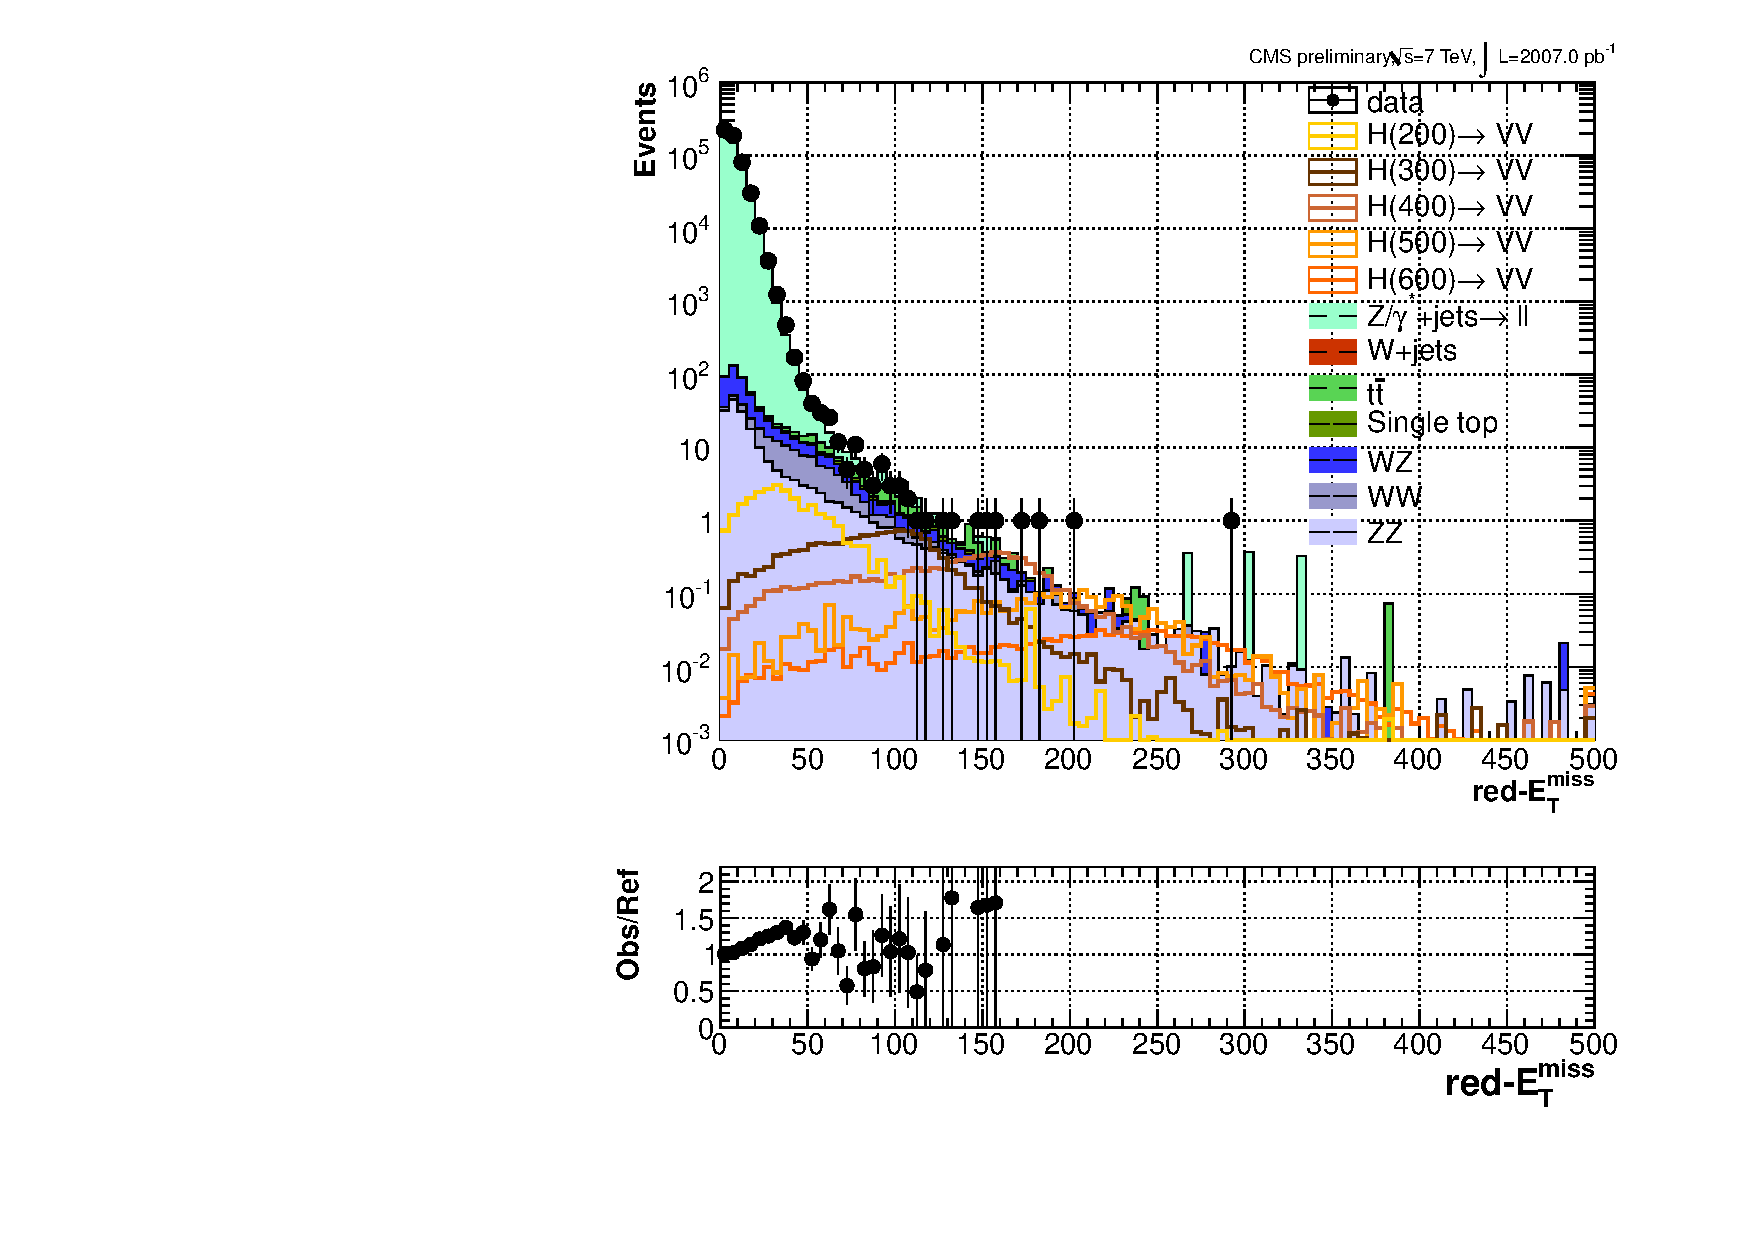
\includegraphics[width=0.45\textwidth]{img/mumu_redMet}
\caption{\RMET distribution in di-muon events.
The original definition from the D0 collaboration is shown on {\em left} to be compared with the definition adopted in this manuscript shown on the {\em right}.}
\label{fig:redmet}
\end{center}
\end{figure}

Fig.~\ref{fig:redmetcomps} shows the distribution of the \RMET longitudinal and transverse components.
As expected the transverse component carries little or no information about the topology of the event
and it is mainly dominated by \MET and jet energy resolution. The longitudinal component however signals the presence of
real \MET in the recoil of the dilepton which becomes more significant for the high mass regime.
As expected the instrumental background contribution, i.e., Drell-Yan, displays identical behavior in both components.
Overall a fair agreement between data and MC is observed for both components and the residual discrepancy may be related
to the jet energy resolution.
The effect can be identified in Fig.~\ref{fig:redmetpercat} which shows the distribution of \RMET for different event categories:
according to the di-lepton flavor and jet multiplicity. The bulk of the residual discrepancy is identified
in events with significant jet activity.

\begin{figure}[htp]
\begin{center}
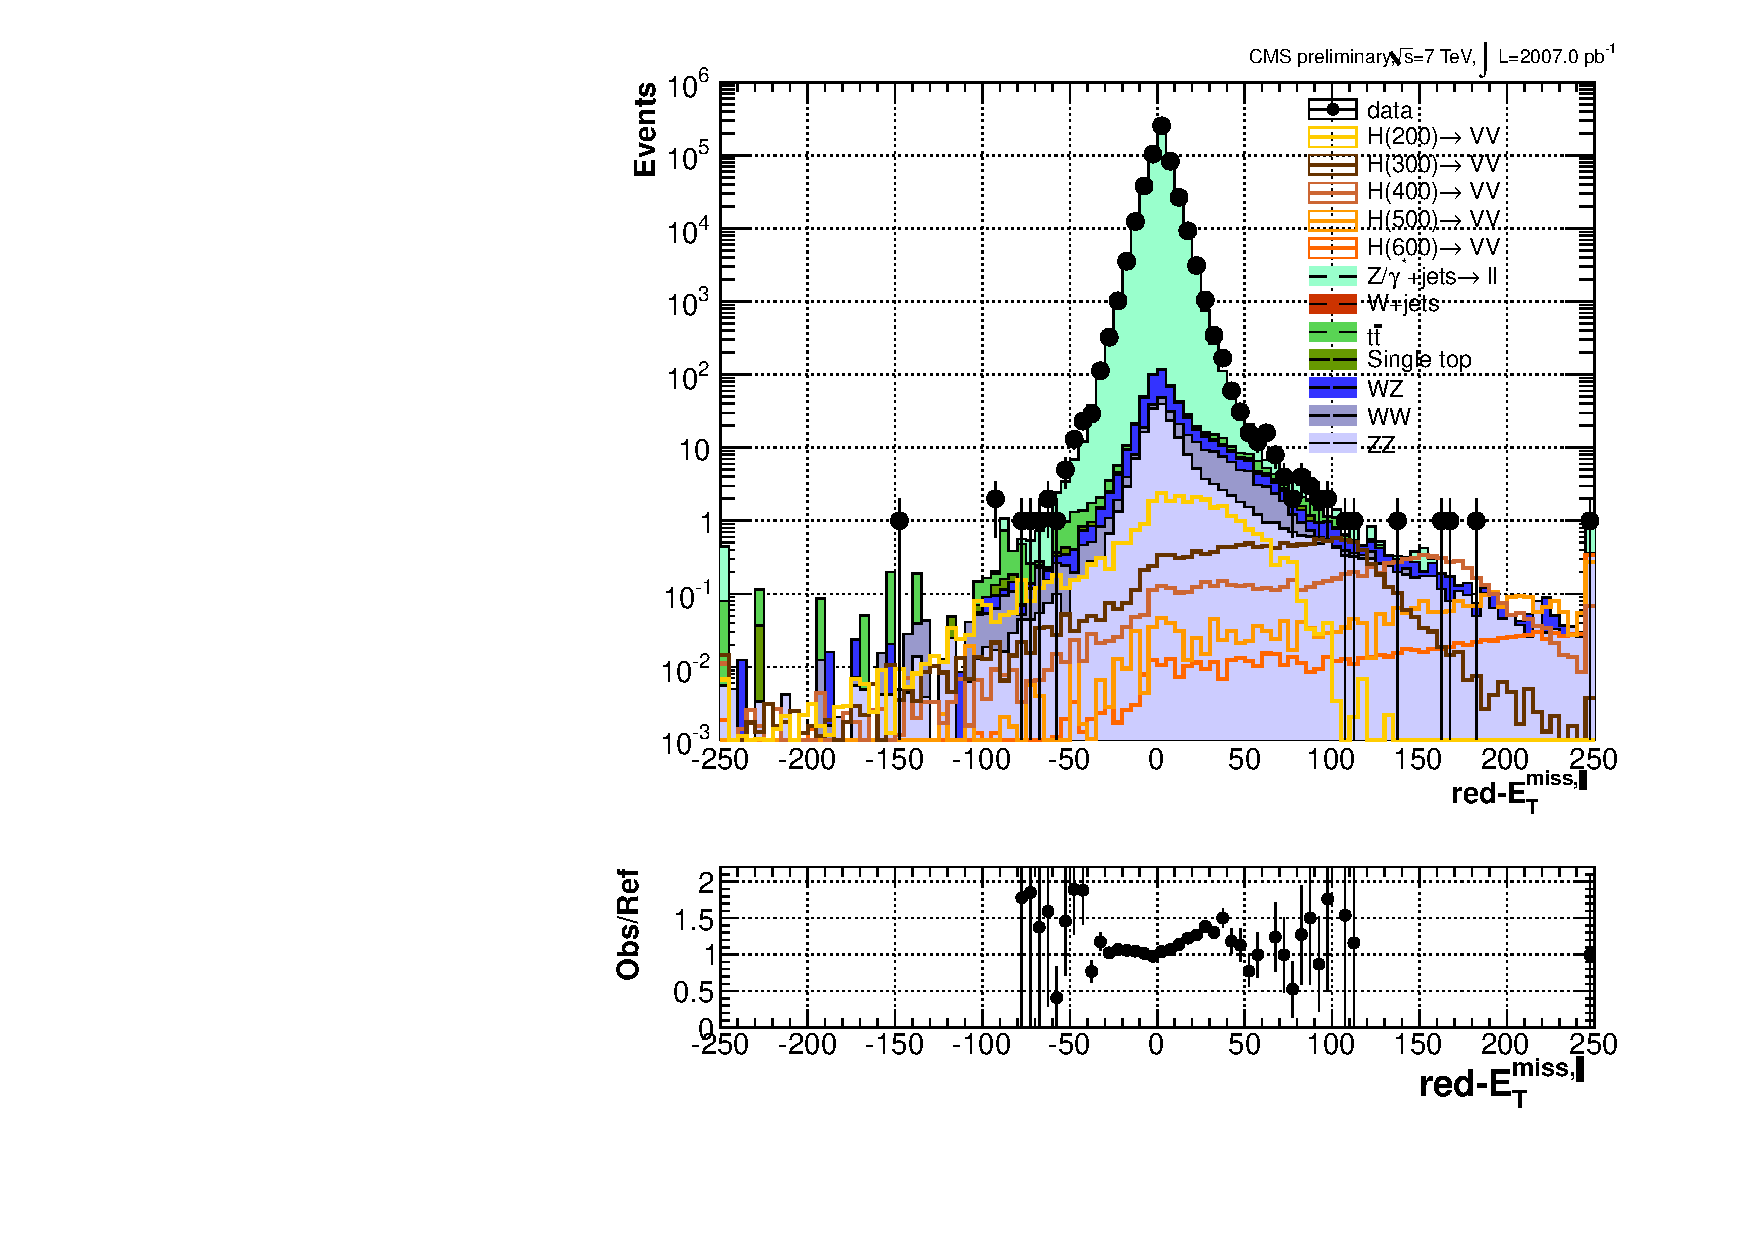
\includegraphics[width=0.45\textwidth]{img/mumu_redMetL}
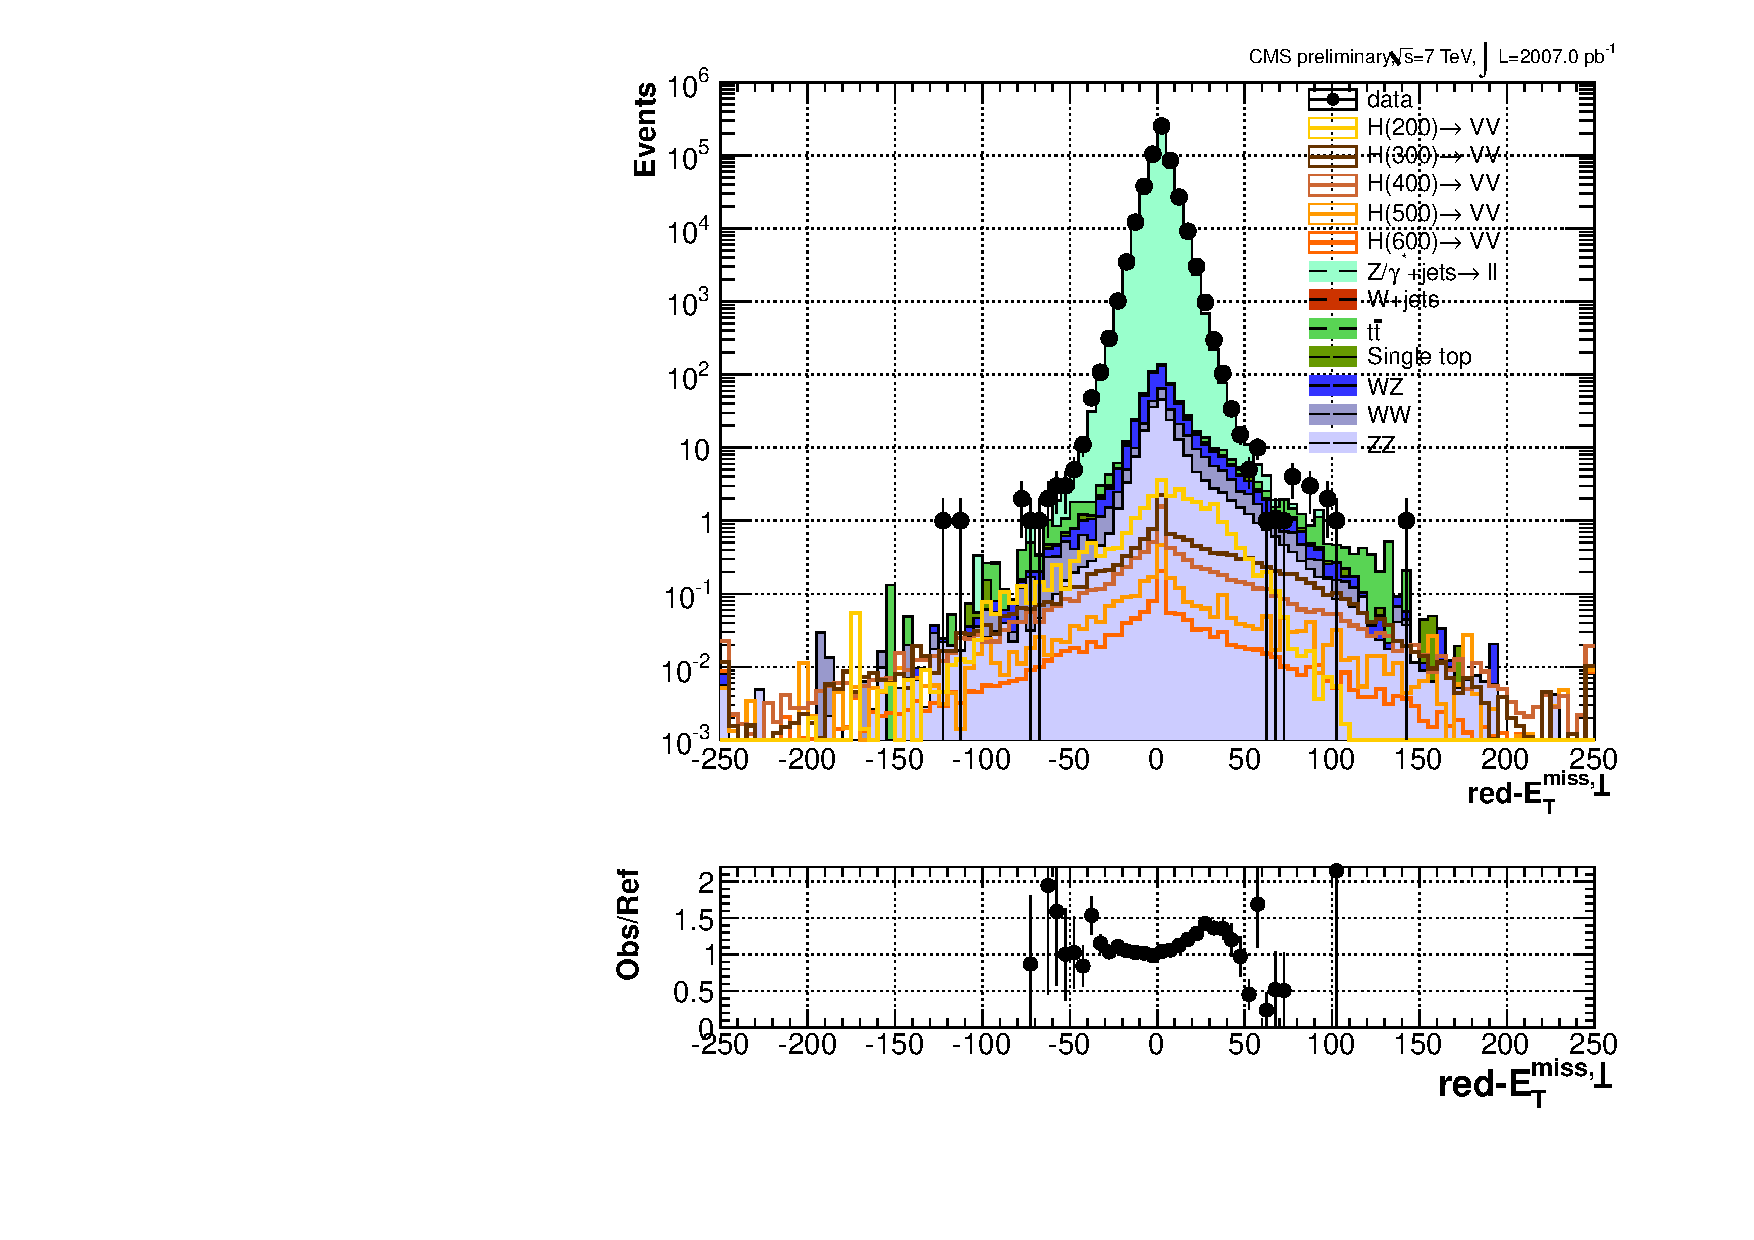
\includegraphics[width=0.45\textwidth]{img/mumu_redMetT}
\caption{\RMET components in di-muon events: longitudinal ({\em left}) and transverse ({\em right}).}
\label{fig:redmetcomps}
\end{center}
\end{figure}


\begin{figure}[htp]
\begin{center}
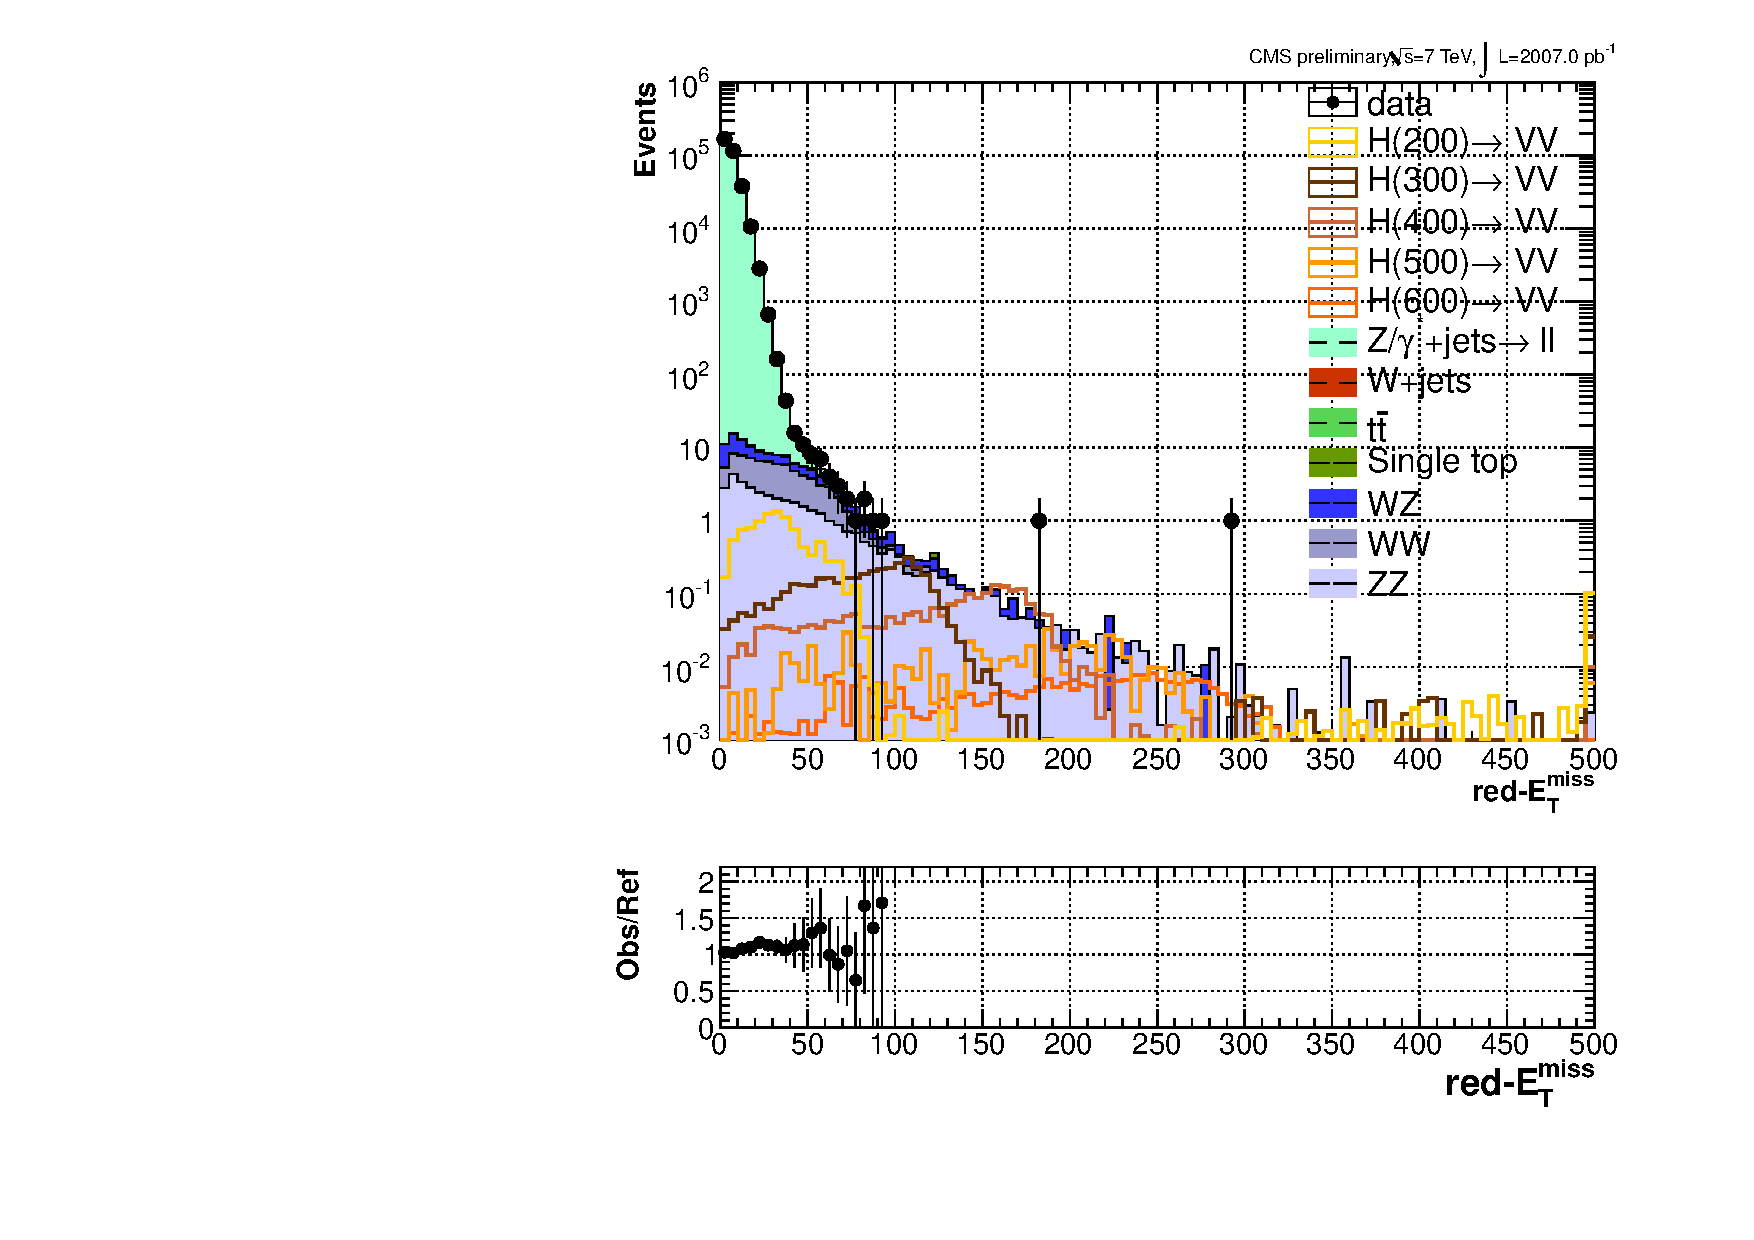
\includegraphics[width=0.24\textwidth]{img/mumueq0jets_redMet}
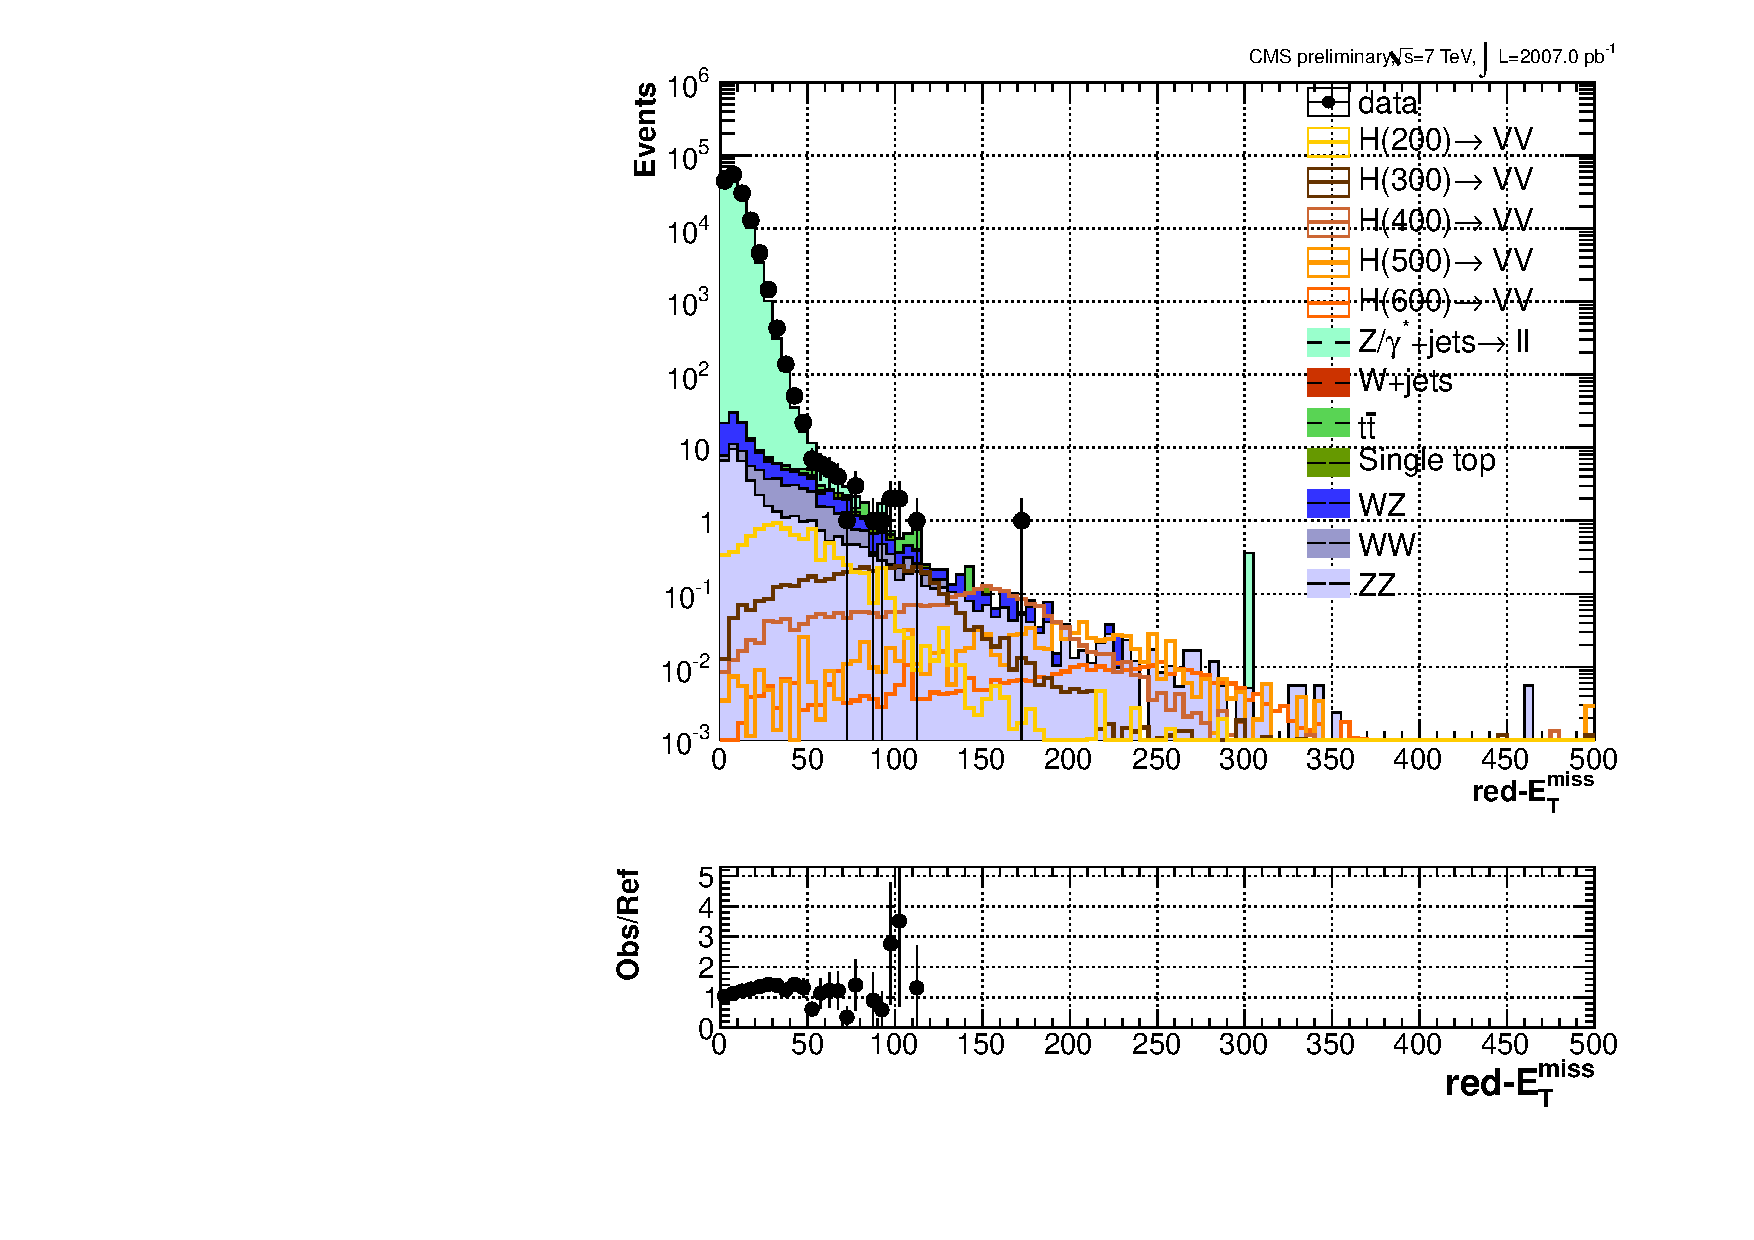
\includegraphics[width=0.24\textwidth]{img/mumueq1jets_redMet}
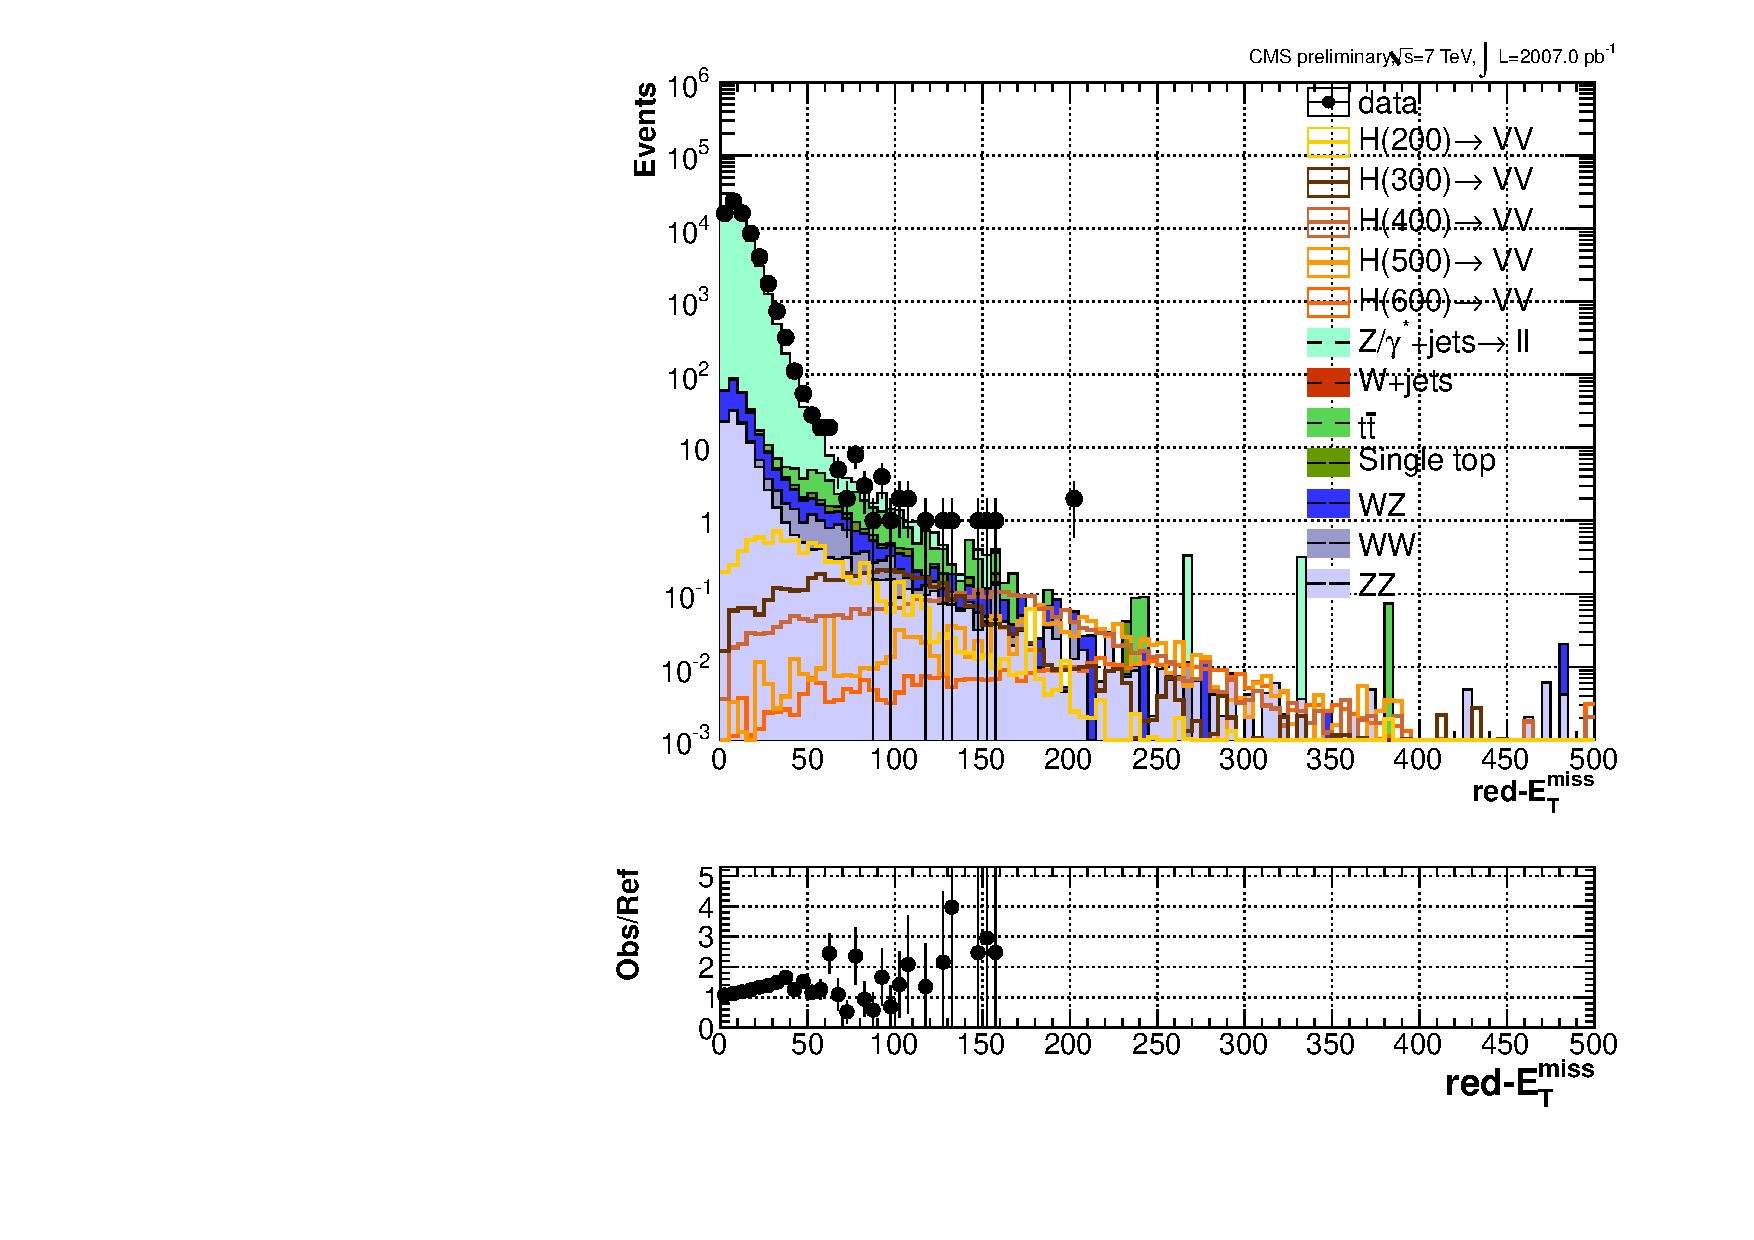
\includegraphics[width=0.24\textwidth]{img/mumugeq2jets_redMet}
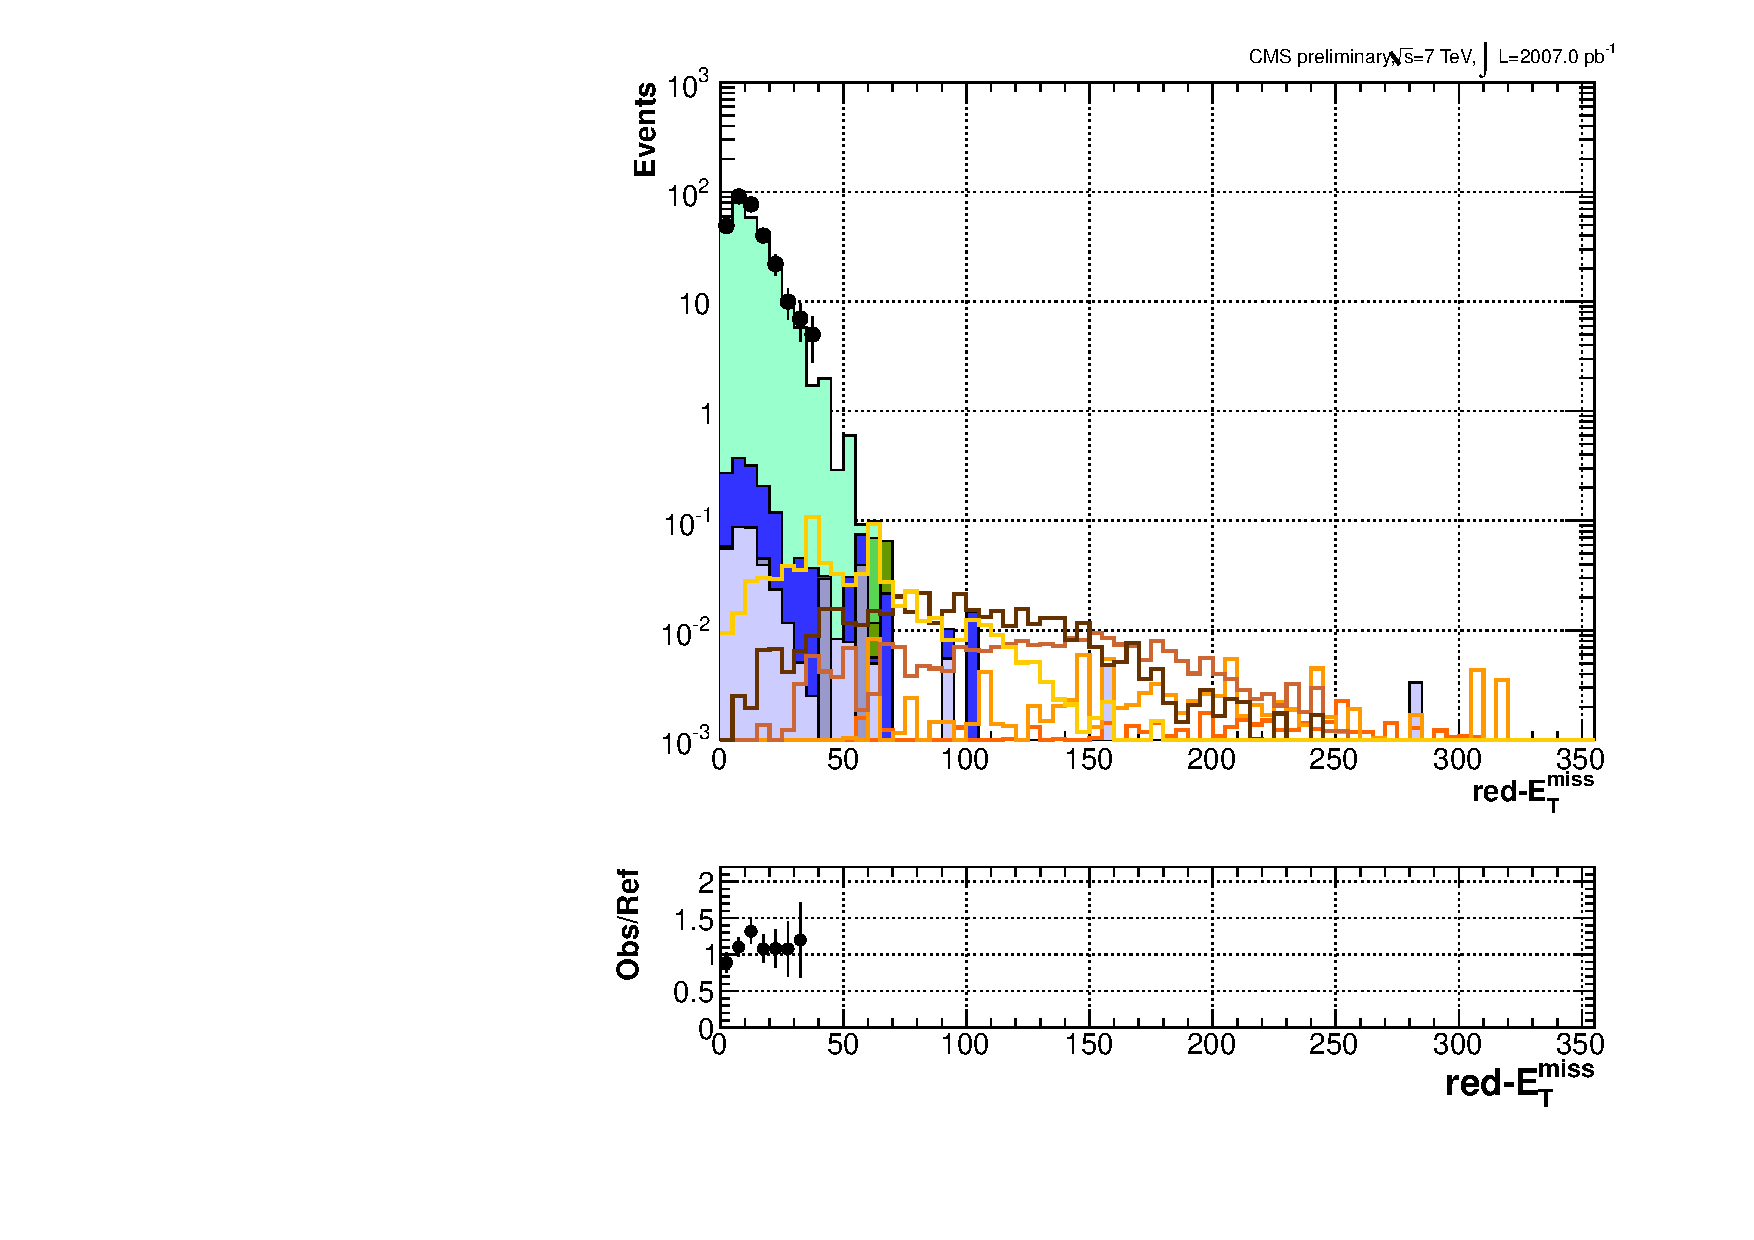
\includegraphics[width=0.24\textwidth]{img/mumuvbf_redMet}\\
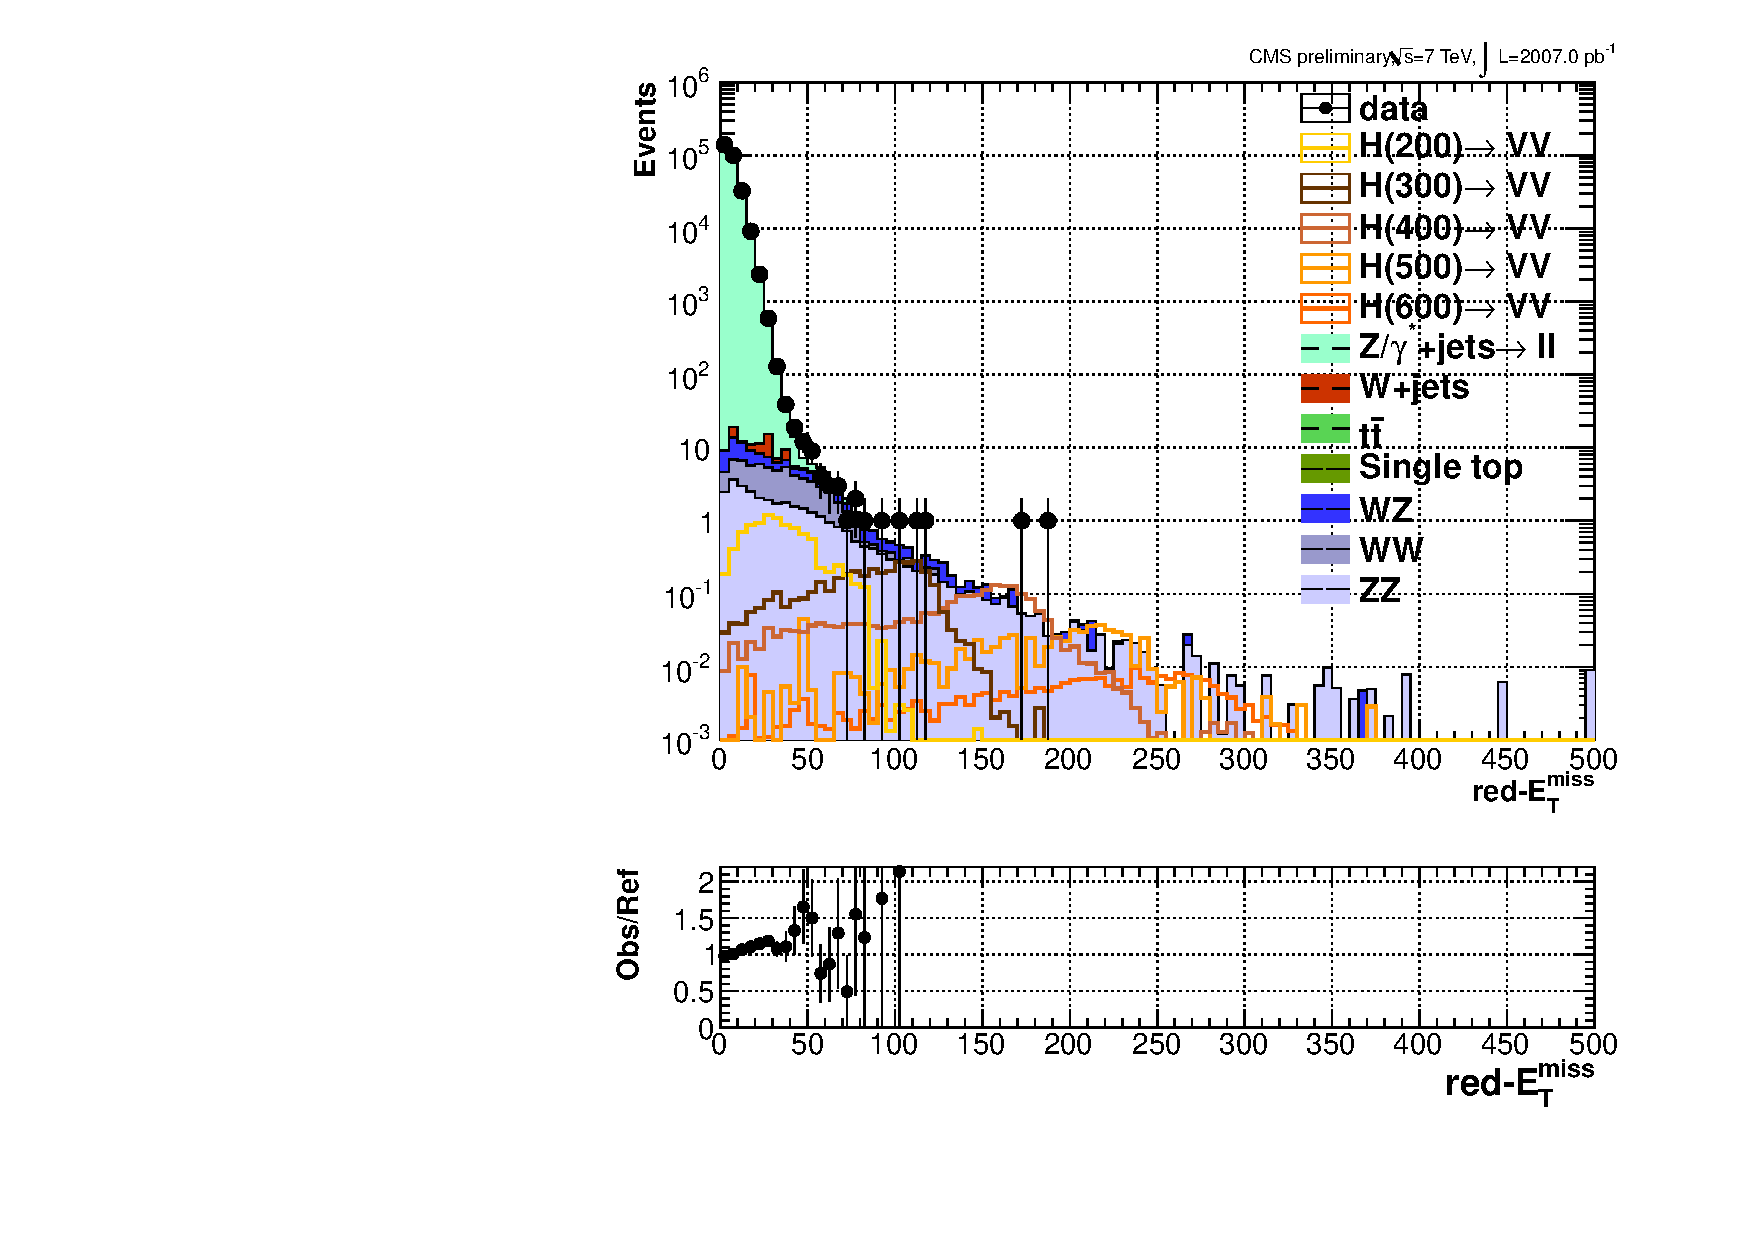
\includegraphics[width=0.24\textwidth]{img/eeeq0jets_redMet}
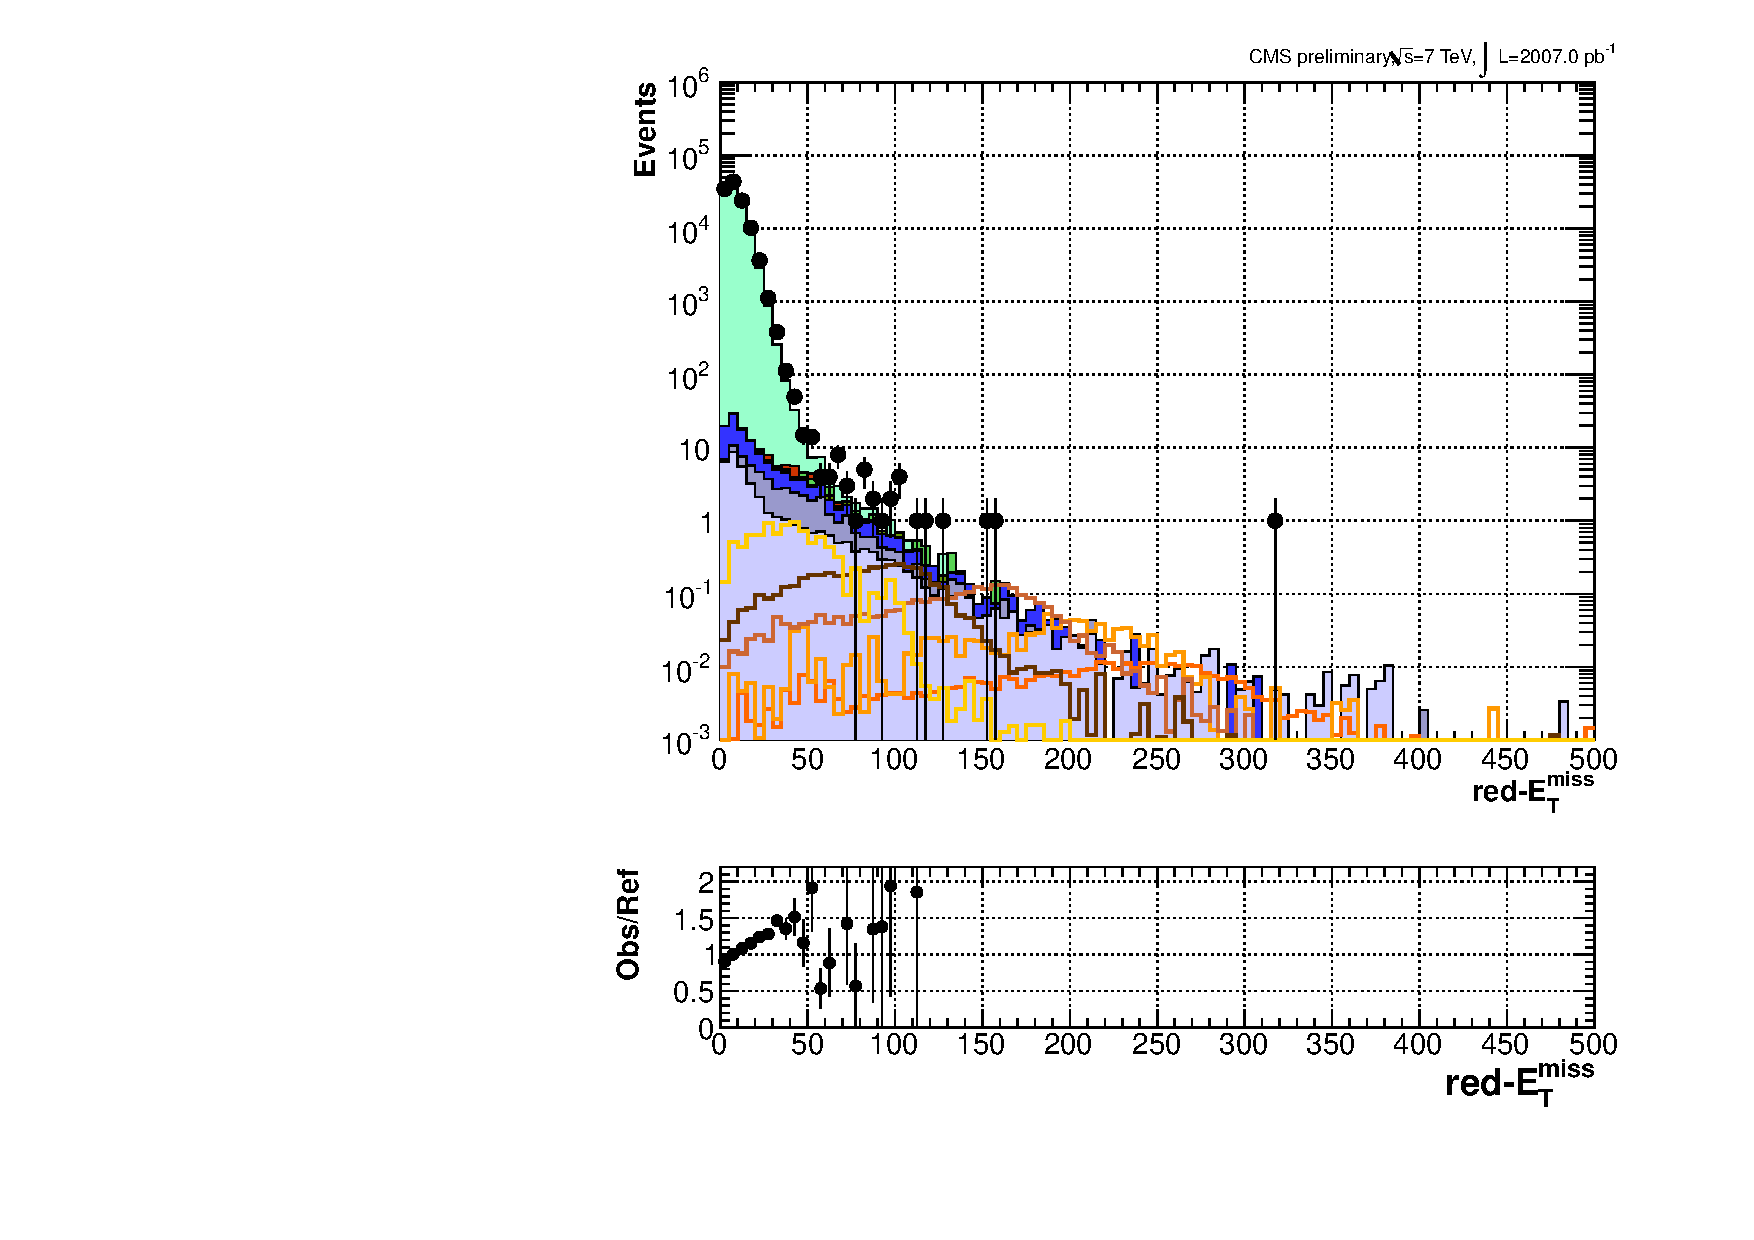
\includegraphics[width=0.24\textwidth]{img/eeeq1jets_redMet}
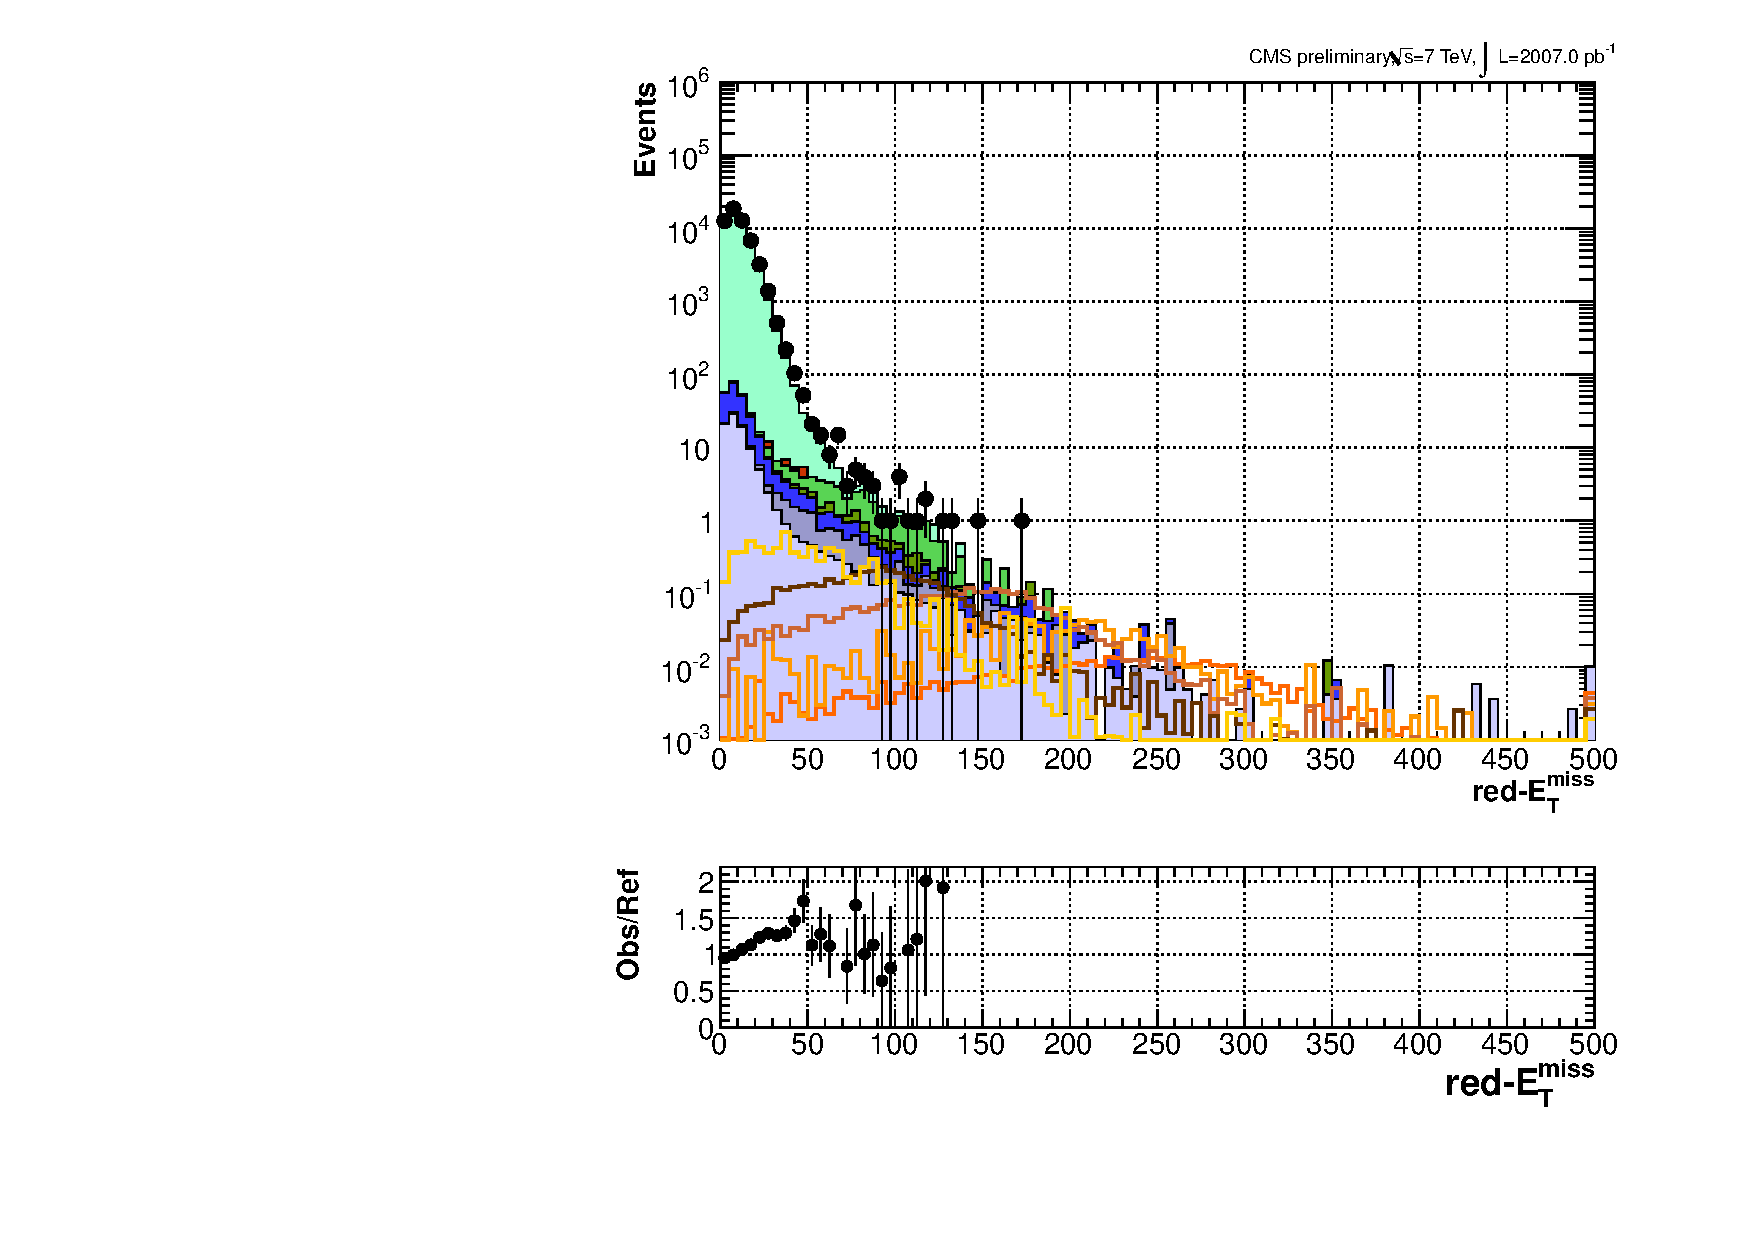
\includegraphics[width=0.24\textwidth]{img/eegeq2jets_redMet}
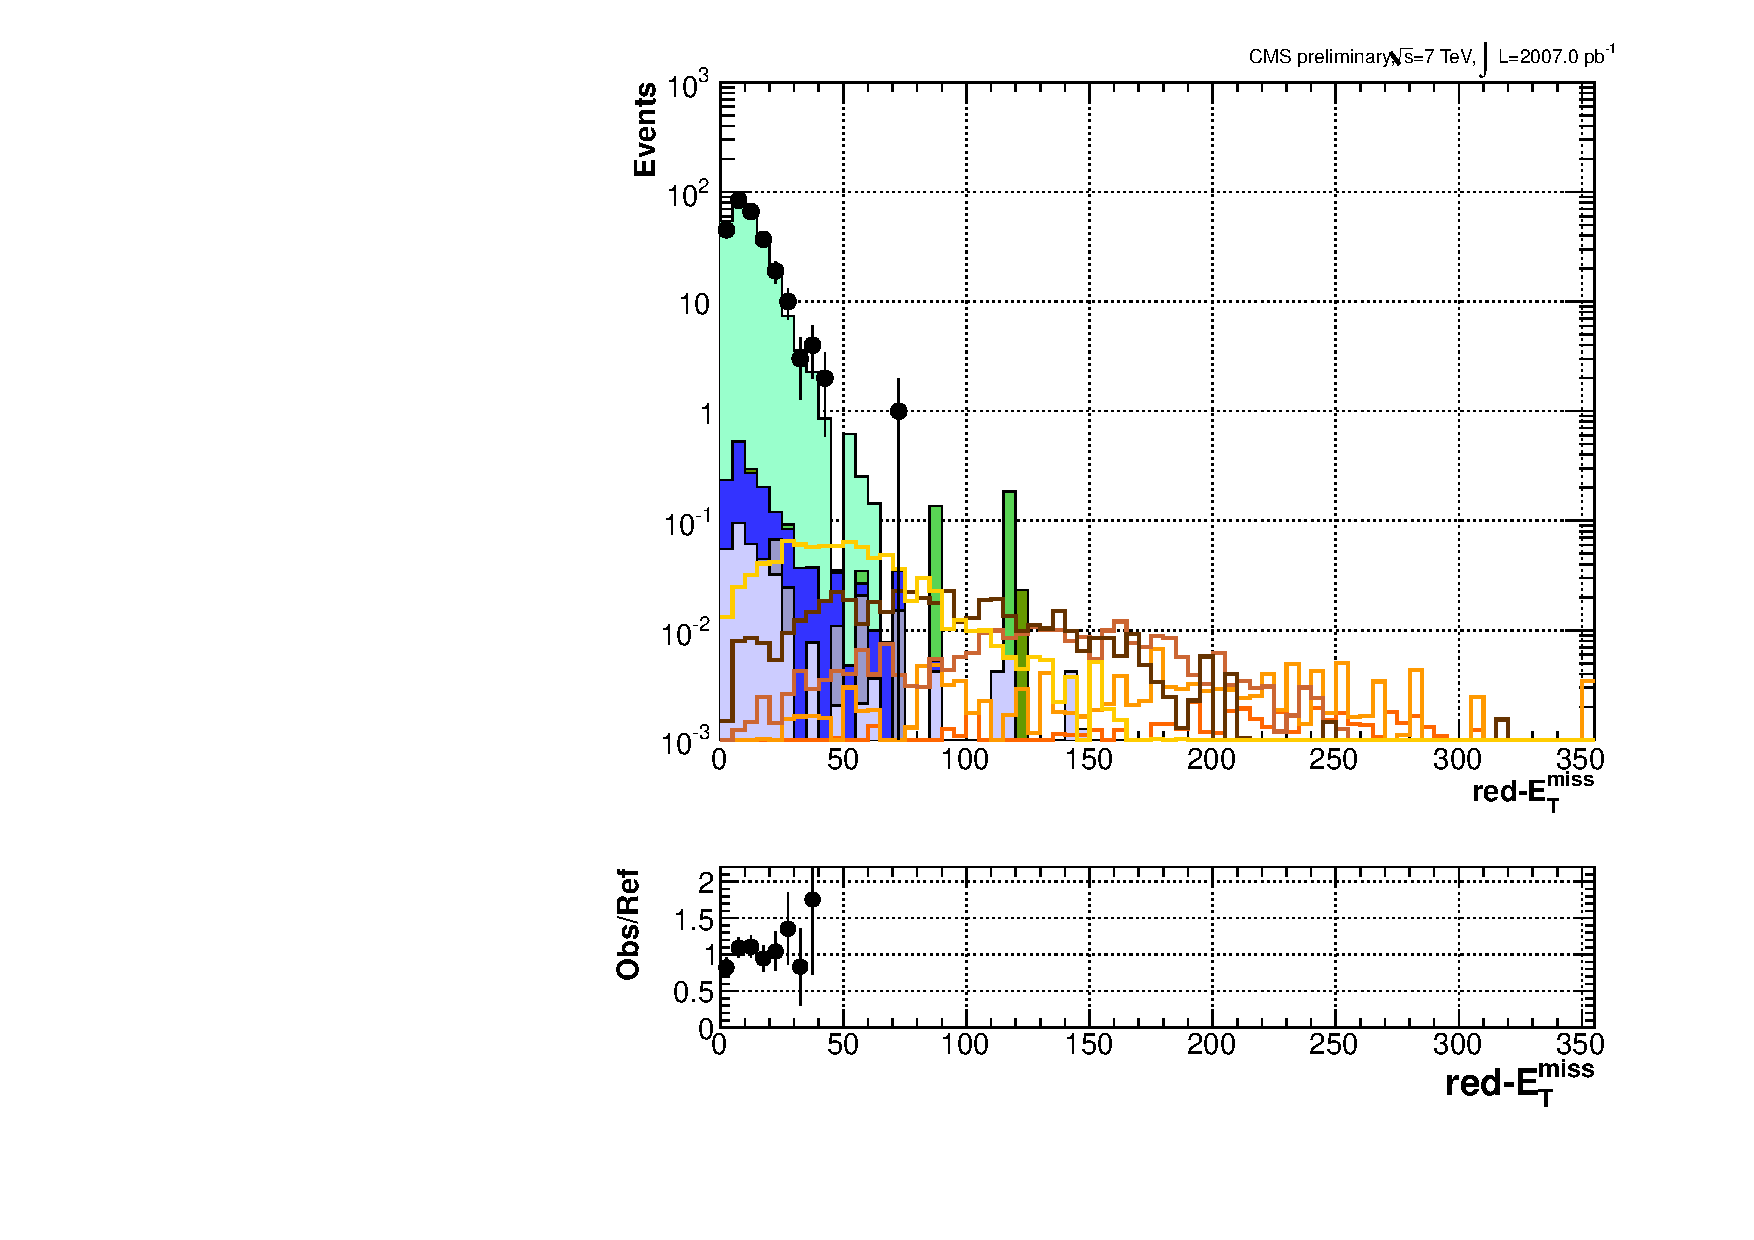
\includegraphics[width=0.24\textwidth]{img/eevbf_redMet}
\caption{\RMET distribution in differen event categories.
From {\em left} to {\em right}:=0 jets,=1 jets, $\geq$2 jets, VBF.
The di-muon (di-electron) channel is shown on {\em top} ({\em bottom}).}
\label{fig:redmetpercat}
\end{center}
\end{figure}

The \RMET variable is adopted in the event selection for the Higgs boson and
two working points (medium and tight) are defined in order to reject the instrumental background ($Z$ events) at a 10$^3$ and 10$^4$ rate level.
The medium (tight) working point is used as a base selection for medium (high) mass search corresponding to 200-300 ($>$300) GeV/c$^2$.
The working points are defined independently for each jet multiplicity bin in order to maximize the rejection power of the instrumental background
\footnote{The working points are obtained from a parameterization of the efficiency curves where the efficiency
is defined from the fraction of events of a given process observed above a given threshold.
The parametrization used is a 2$^{nd}$ order polynomial function of the logarithm of the \RMET cut.}.
Table~\ref{tab:redmetwp} summarizes the values adopted for the medium and tight \RMET working points.
For the VBF category a single (medium) working point is chosen: \RMET$>$57.4~GeV.

\begin{table}[htp]
\caption{Working points for different Drell-Yan rejection powers for \RMET.
The expected efficiency for the selection of different Higgs masses is shown for reference.}
\label{tab:redmetwp}
\begin{center}
\begin{tabular}{lccc} \hline\hline
Jet multiplicity      & =0 jets & =1 jets & $\geq$ 2 jets  \\\hline
                      &         &         & \\\hline
\multicolumn{4}{c}{{\bf Medium working point} ($10^{-3}$ rejection factor)} \\\hline
Cut value             & 30.5    & 38.8    &  50.8\\
$\varepsilon$(200)    & 59.7\%  & 52.5\%  &  41.6\% \\
$\varepsilon$(300)    & 91.2\%  & 88.5\%  &  81.1\% \\
$\varepsilon$(400)    & 94.8\%  & 93.2\%  &  90.2\% \\\hline
                      &         &         & \\\hline
\multicolumn{4}{c}{{\bf Tight working point} ($10^{-4}$ rejection factor)} \\\hline
Cut value             & 39.0    & 52.4    &  78.7\\
$\varepsilon$(200)    & 38.9\%  & 32.3\%  &  17.8\%\\
$\varepsilon$(300)    & 87.6\%  & 79.5\%  &  53.1\%\\
$\varepsilon$(400)    & 91.2\%  & 89.1\%  &  81.3\% \\\hline\hline
\end{tabular}
\end{center}
\end{table}

The performance of the \RMET can be further quantified relatively to the standard \MET measurement 
as well as other \MET related variables. The \MET measurement can be made more robust against pileup contamination
by considering the minimum of two transverse momenta sums: of all particle flow candidates (\MET) or of all 
charged particle flow candidates which can be associated to the primary vertex of the event (\assocChMET).
This variable was introduced in Section~\ref{subsec:trigrec} to characterize the properties of the primary vertex.
As it is built using a vertex constraint it is expected to have a small contamination from pileup.
It's resolution is however degraded and has a non trivial dependence on the topology of the event,
therefore the minimum is taken with respect to the full \MET measurement.
A third variable which is worth comparing to is the projected missing transverse energy (\projMET)
which aims at minimizing the poor reconstruction of leptons.
Even if this is not considered to be the main problem affecting the \MET measurement under the $Z$ boson peak
we compare its performance with the other measurements.
This variable is computed as the transverse component of \MET 
relatively to the closest lepton (if closer than $\pi/2$ in the azimuthal angle)
or the full \MET otherwise
\footnote{\projMET can be explicitly written from the following formulas.
Let $\delta\phi^{\rm min}=\min\{\delta\phi(E_{T}^{miss},l^1),\delta\phi(E_{T}^{miss},l^2)\}$
be the azimuthal angle between the \MET vector and the transverse momentum of the closest lepton.
Then \projMET=\MET$\cdot\sin\delta\phi^{\rm min}$ if $\delta\phi^{\rm min}<\pi/2$ or \MET, otherwise.}.
Following the prescription adopted by~\cite{CMS-PAS-HIG-11-003}
the dependency on pile-up is reduced by taking the minimum \projMET computed from \MET and \assocChMET.
This minimization exploits further the correlation between both estimates in signal and 
uncorrelation otherwise, as in Drell-Yan events.
Fig.~\ref{fig:metperformances} summarize the performance of each variable 
for the rejection of the instrumental background considering two hypothetical higgs boson masses.
The performance is compared for events selected under the $Z$ boson peak and in the side-band region, i.e.
dilepton events with a mass compreehended in the 61-76 and 106-121 GeV/c$^2$ range.
It is visible that the \RMET approach is performing better overall in the $Z$ boson peak region which is the region of interest for our study.
The performance of the \RMET variable is significantly better in the low mass regime under the $Z$ mass peak.

\begin{figure}[htp]
\begin{center}
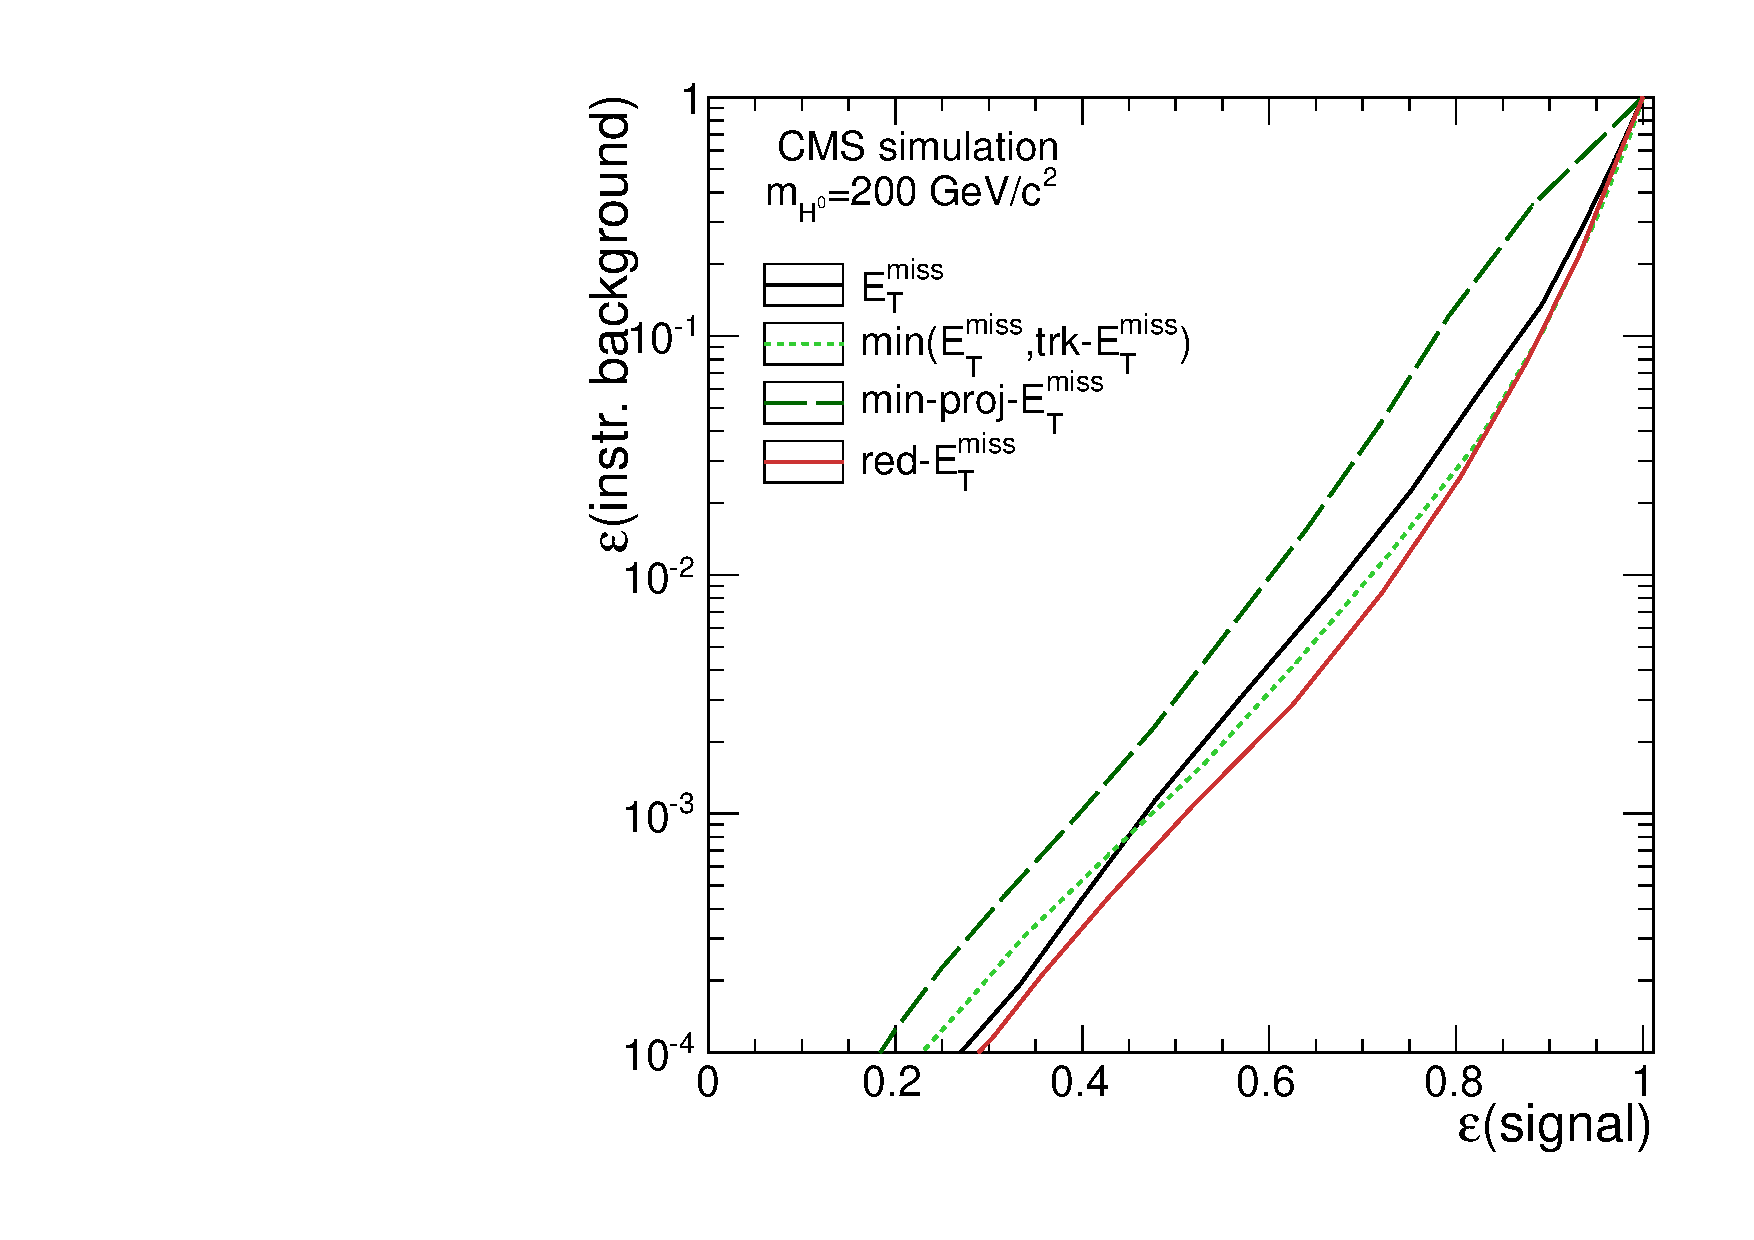
\includegraphics[width=0.4\textwidth]{img/eff200}
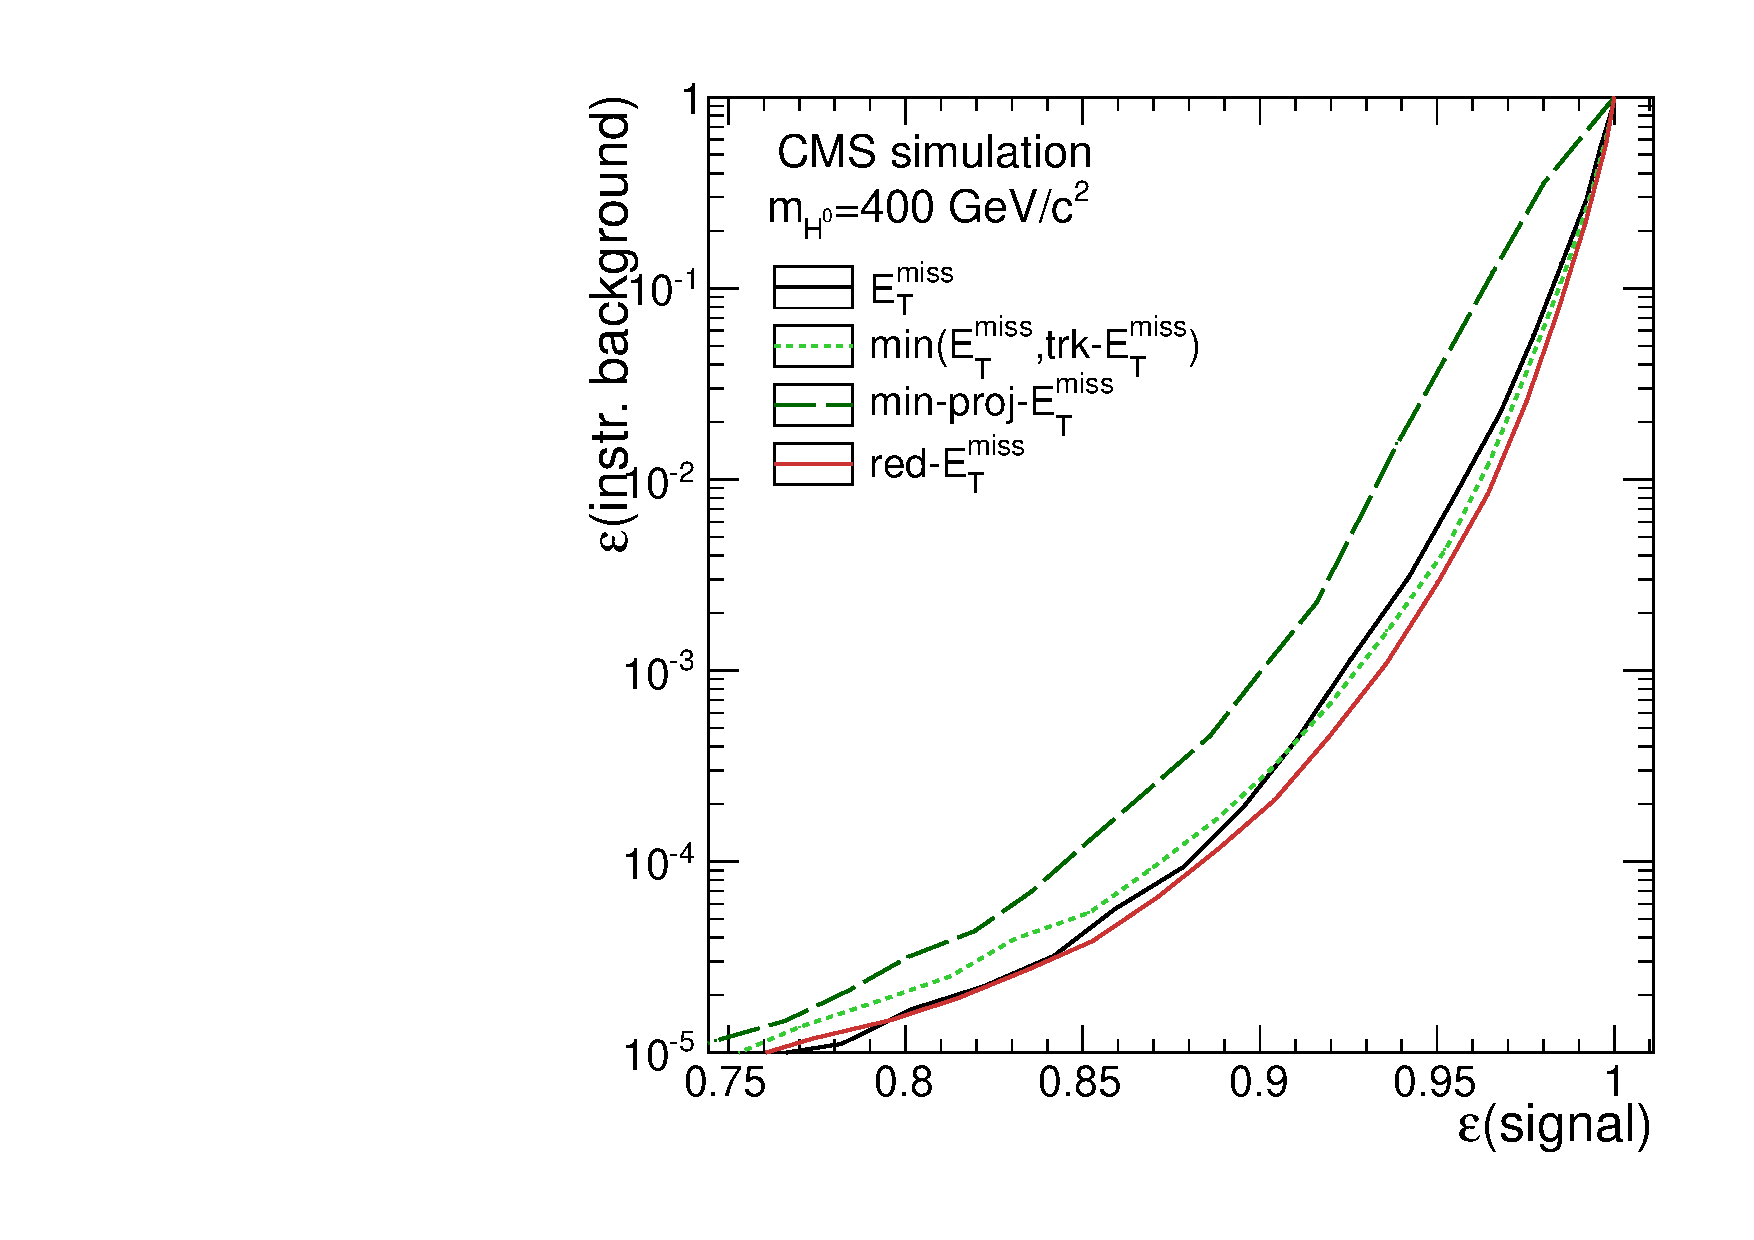
\includegraphics[width=0.4\textwidth]{img/eff400}\\
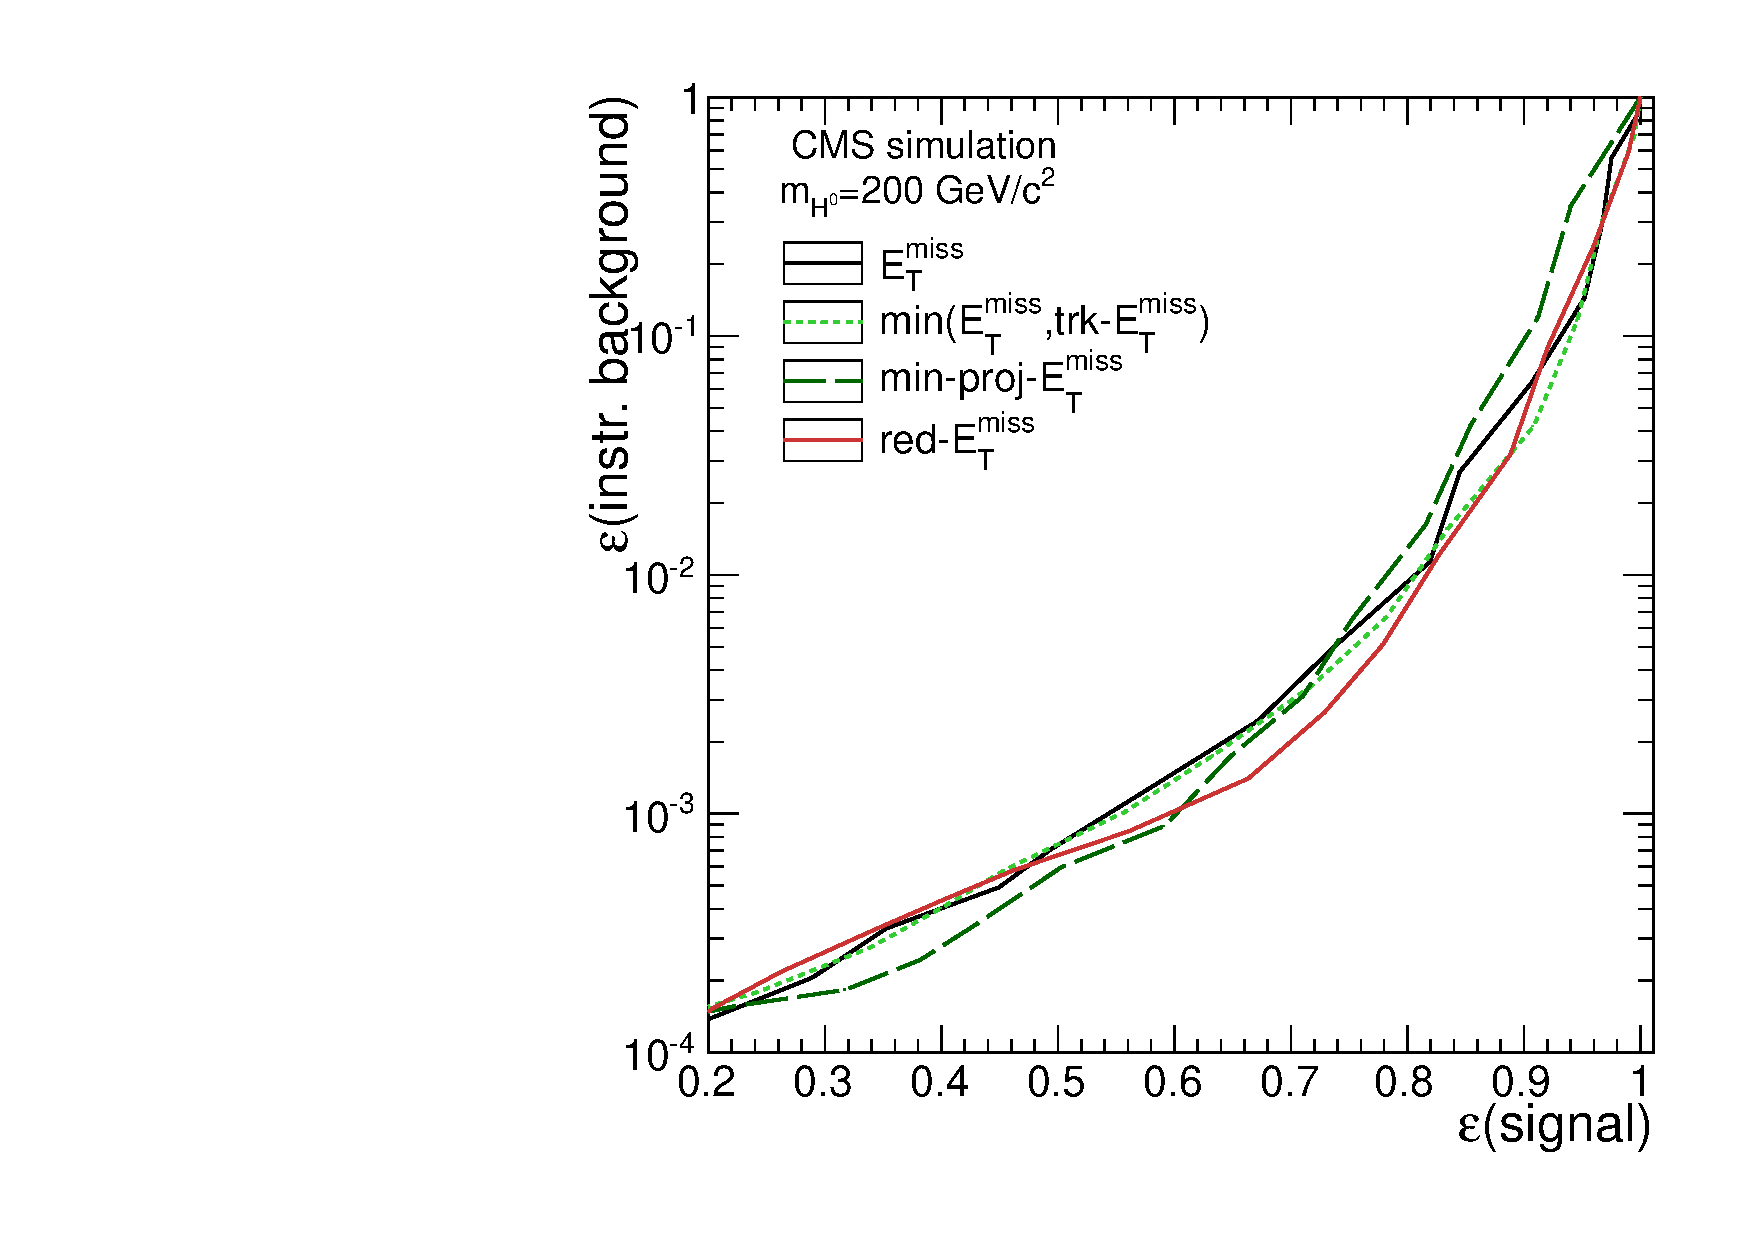
\includegraphics[width=0.4\textwidth]{img/eff200_zsideband}
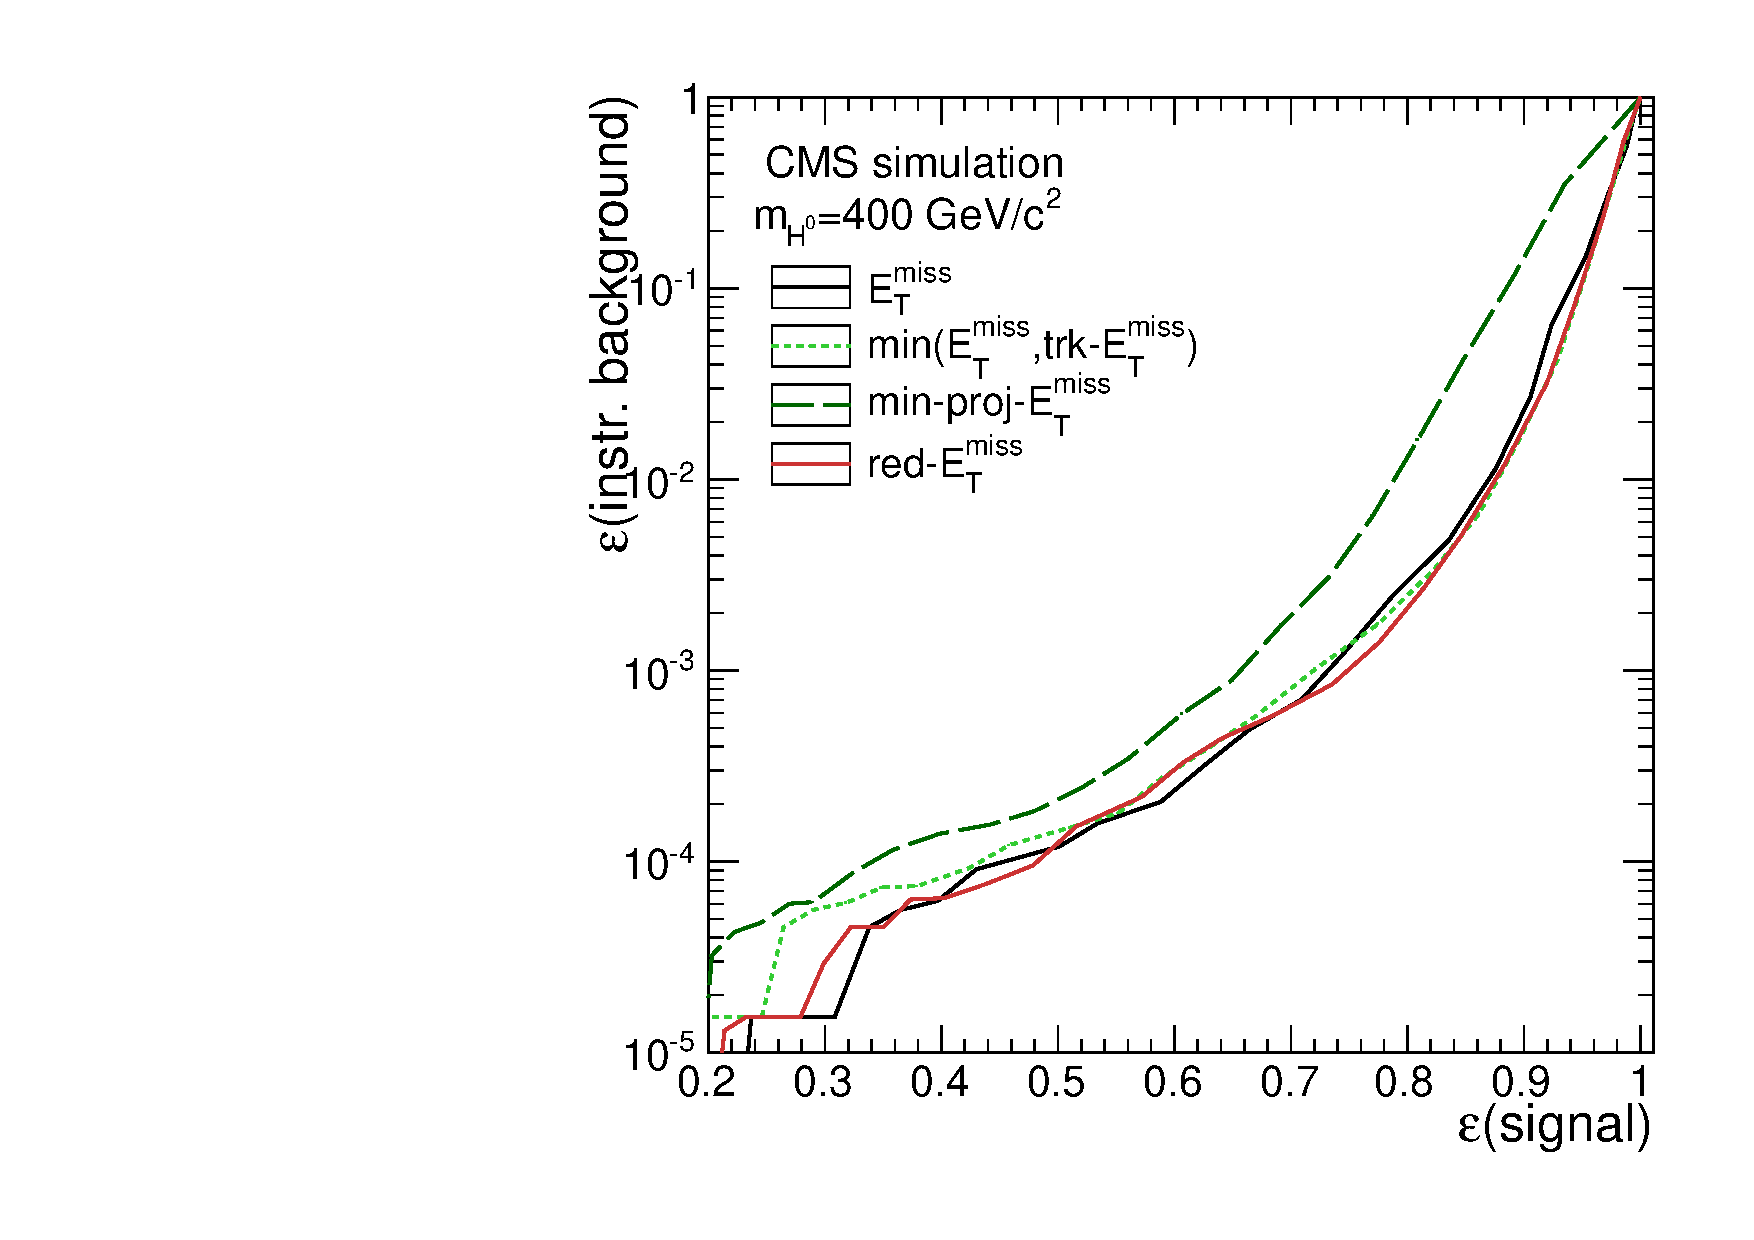
\includegraphics[width=0.4\textwidth]{img/eff400_zsideband}
\caption{Efficiency curves for signal versus instrumental background acceptance for different \MET variables.
Signal is considered as a 200~GeV/c$^2$ ({\em left}) or a 400~GeV/c$^2$ ({\em right}) Higgs boson.
The {\em top} plots show the results obtained in the Z-boson mass region while the {\em bottom} plots show the results obtained in the side-band region.}
\label{fig:metperformances}
\end{center}
\end{figure}

The performances can be further compared in terms of robustness against the variation of the pileup scenario.
This test is summarized in Fig~\ref{fig:metperformancevspileup}. 
We conclude that all approaches have a dependency on the pileup scenario which is minimized when taking
the \assocChMET or \RMET approaches. The dependency for these pseudo-\MET variables is observed to be approximately linear
in both the average and RMS of the spectrum.

\begin{figure}[htp]
\begin{center}
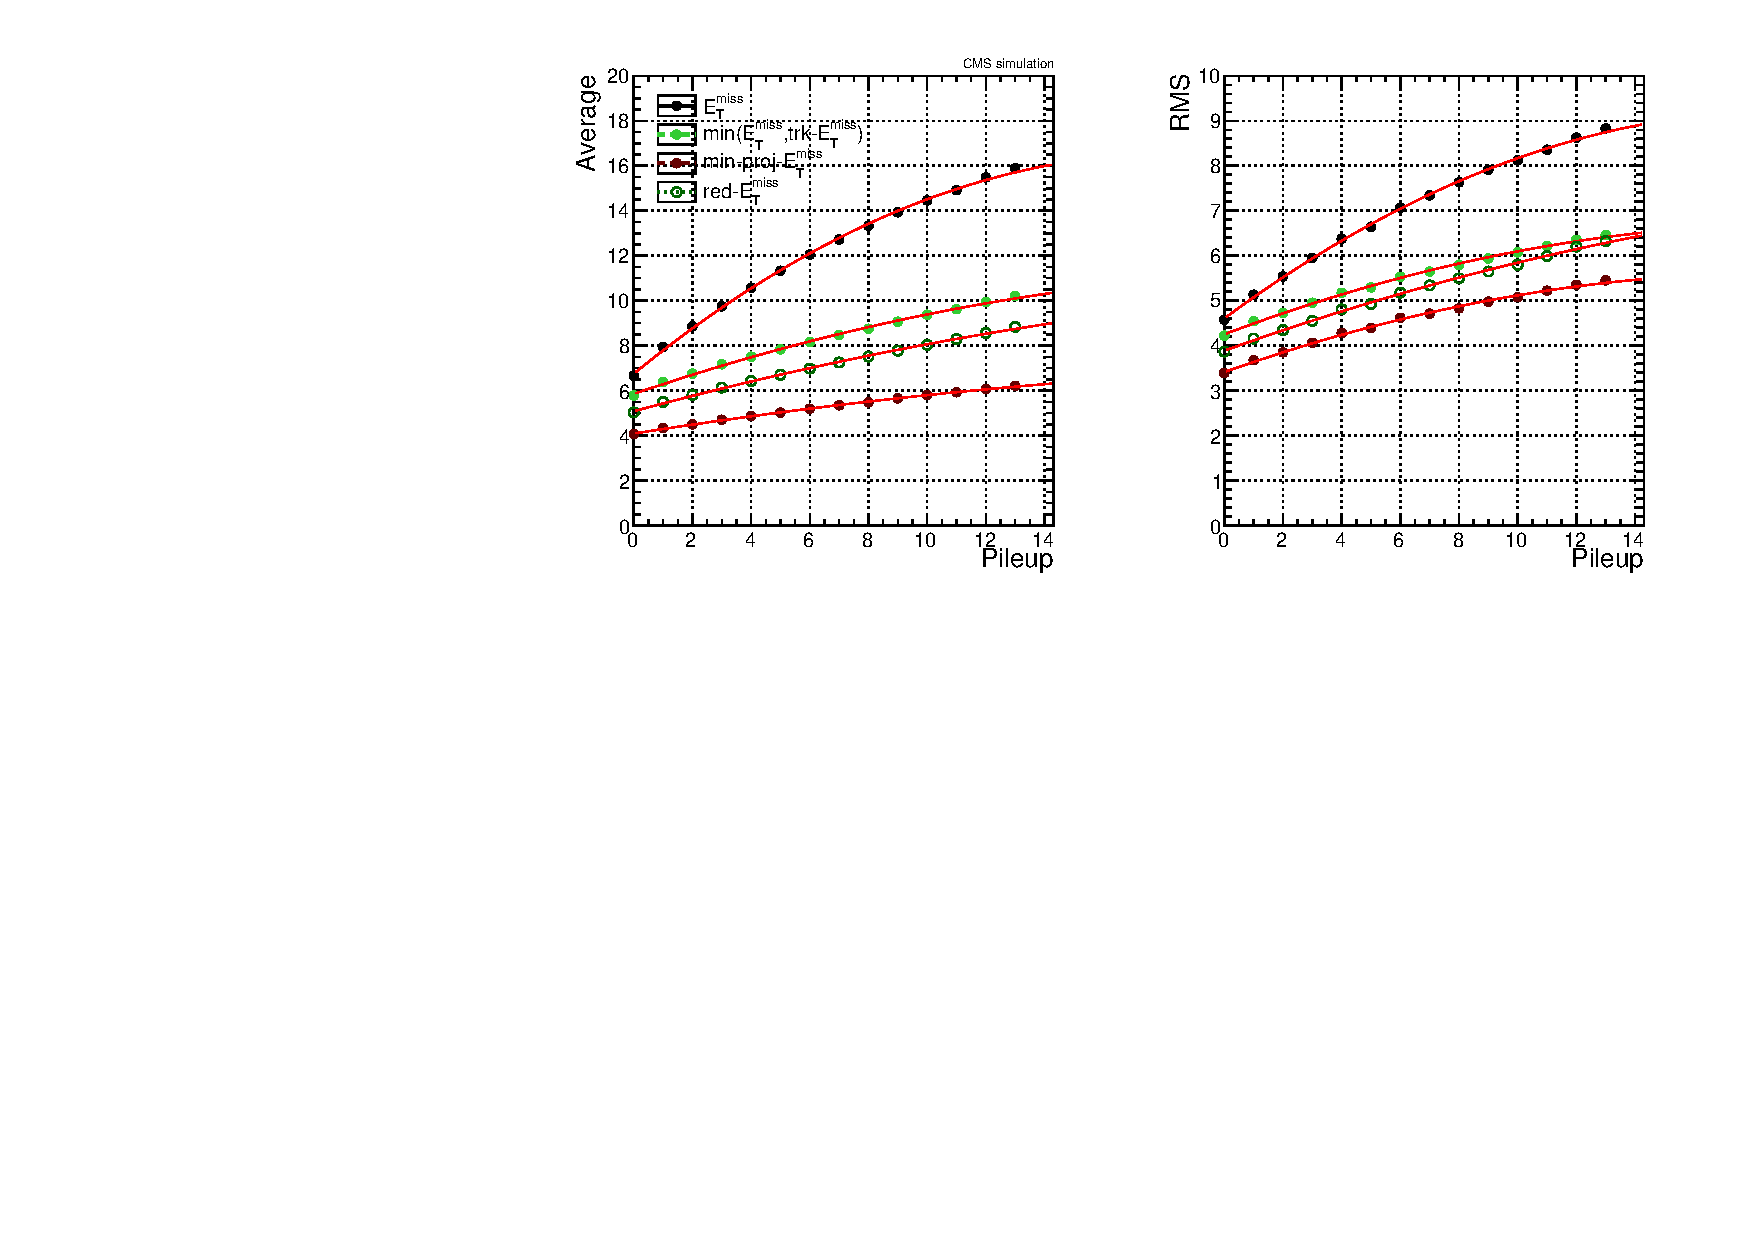
\includegraphics[width=0.9\textwidth]{img/metvariablesVsPileup}\\
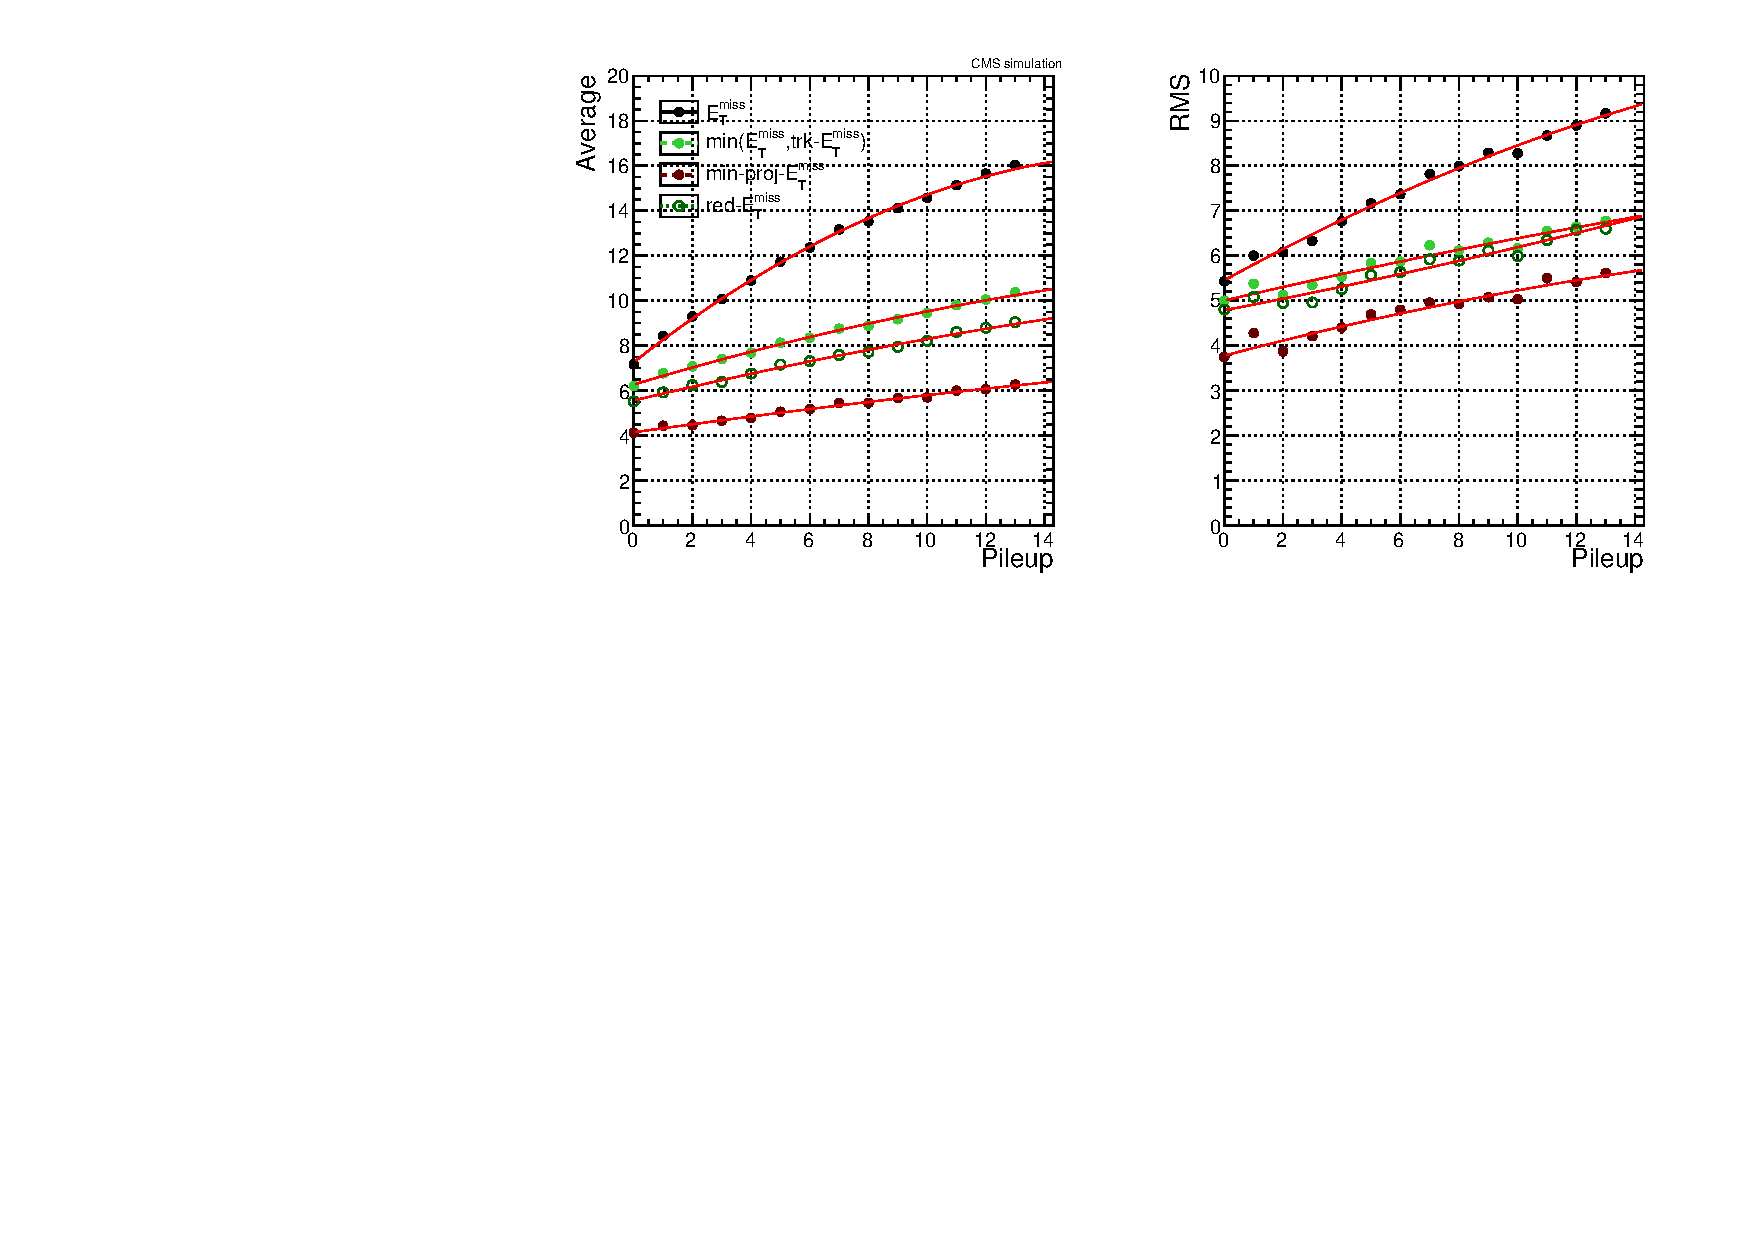
\includegraphics[width=0.9\textwidth]{img/metvariablesVsPileup_zsideband}
\caption{Average ({\em left}) and RMS ({\em right}) of the distribution of different \MET related variables in $Z/\gamma^{*}\rightarrow ll$ events, as function of the pileup.
The {\em top} plots show the results obtained in the Z-boson mass region while the {\em bottom} plots show the results obtained in the side-band region.}
\label{fig:metperformancevspileup}
\end{center}
\end{figure}

In the next sub-section we discuss further strategies which are still subject of on-going studies which attempt 
to minimize further the dependence of these variables against pileup.

%%%
%%% Pileup
%%%
\subsection{Description of the FastJet-based clustering method}
\label{subsec:fjpucontrol}

In the previous section it was noticed that by taking the minimum of the \MET measurement and the \assocChMET measurement for each event
we can obtain an estimate of the \MET which is more robust against the contamination from pileup.
The drawback of this approach is the loss of resolution in the measurement as \assocChMET uses only the charged component of the event
which can be measured up to a pseudo-rapidity of $|\eta|<$2.4 due to the limited acceptance of the tracker.
However for the signal we're interested in we expect that the neutrinos are indeed emitted in the central region of the detector
and therefore we expect a correlation between \MET measured using the information from the full detector and \MET measured using the central region.
For instrumental background this is not the case any longer, as depicted in Fig.~\ref{fig:metcorrelations} ({\em top}).
In this section we explore further this correlation and develop a strategy to control further the measurement of \MET using the
more detailed information on the (im)balance of the event in the transverse plane, namely 
using regional and \MET composition information.

As we have noticed in Sec.~\ref{subsec:trigrec} \pfMET is reconstructed from the sum of the transverse momentum of all reconstructed particle flow candidates 
using the full CMS detector acceptance. This procedure ensures that we are using the most complete energy flux information experimentally available.
It also relies on the fact that, if present, pileup events are expected to contribute with smaller amount of energy flux which is expected to be balanced
as these events are mostly minimum bias so that in the end \pfMET is the most unbiased estimator of the \MET produced by the primary interaction.
Besides detector acceptance, resolution, material effects, dead regions, out of time pileup also contributes in a non negligible way to the degradation of the \MET measurement.
Therefore we adopt a tracker-driven strategy to cluster both charged and neutral candidates starting from the reconstructed vertices. 
This strategy is of course limited by construction by the tracker acceptance and reconstruction efficiencies (i.e. $|\eta|<$2.4) but has the potential
of refining the information on whether a given particle flow candidate should or should not be associated to the primary interaction even if it is neutral.
Moreover, taking into account that the sources of real \MET should be produced within the central part of the detector, this approach should be able to 
discriminate central sources of \MET from mis-reconstruction/calibration of the most forward calorimeters or from the extreme contamination from pileup.

We have chosen to follow the approach summarized below:

\begin{enumerate}
\item{\bf Vertex association} - we associate all charged particle flow candidates to a single reconstructed vertex in the event. The association is 
done based on the weight which each track has in the vertex reconstruction fit. The vertex for which the track has highest weight is chosen.
In case the track was not used in any vertex fit (or in the case where the track has the same weight for two different vertices), the vertex is chosen
by minimizing the distance along the beam pipe, i.e. $\Delta z$.

\item{\bf FastJet clustering} - for each vertex the collection of associated charged particles is used to build jets using the FastJet algorithm~\cite{Cacciari:2006sm}.
The anti-$k_T$ algorithm is used. Different cone parameters ($R=$0.5, 0.7, 1.0) and different jet $p_T$ thresholds ($p_T>$2, 5 GeV/c) are used for study.

\item{\bf Neutral clustering} - the charged jets are used to project cone areas with an aperture $\Delta R$ corresponding to the cone parameter used in the jet clustering.
Neutral particle flow candidates found inside these areas are considered to be associated to the same vertex as the one from which the jet was seeded.
To prevent double counting the association of neutrals starts from the primary vertex and proceeds by decreasing order of $\sum p_T^2$ of the vertices.
Once the neutral candidate is associated it is removed from the list of particles to be associated.

\item{\bf \MET computation} - using the particles associated to each vertex an estimate of the \MET per reconstructed is obtained. The vertex-\MET estimates are restricted to $|\eta|<2.4$.
\end{enumerate}

Table~\ref{tab:pumettypes} summarizes the usage of the different clustered components in order further the \MET computation.
Three extra \MET types are defined: residual (\assocOvMET) built from all the candidates associated to secondary vertices,
clustered (\assocMET) built from all the candidates associated to the primary vertex and clean (\cleanMET) computed
from removing from the standard \MET the candidates associated to other vertices.

\begin{table}[htp]
\caption{Definitions used for the different \MET approaches compared in this study.
The particles (not) used in the computation of each \MET type are signaled with $\blacksquare$ ($\Box$). 
pVtx (oVtx) is used as a shorthand for primary (other) vertex(ices). }
\label{tab:pumettypes}
\begin{center}
\begin{tabular}{lcccccc} \hline\hline
\multirow{3}{*}{Particles} & \multicolumn{3}{c}{\bf Charged}                    & \multicolumn{3}{c}{\bf Neutral}                       \\  
                           & all             & \multicolumn{2}{c}{associated}   & all                             & \multicolumn{2}{c}{associated} \\
                           & ($|\eta|<$2.4)  & pVtx           & oVtx            & ($|\eta|<$5)                  & pVtx           & oVtx \\\hline
\MET                       & $\blacksquare$  &                &                 & $\blacksquare$                &                &                \\\hline
\centralMET                & $\blacksquare$  &                &                 & $\blacksquare$ ($|\eta|<$2.4) &                &                \\\hline
\assocChMET                &                 & $\blacksquare$ &                 &                               &                &                \\\hline
\assocMET                  &                 & $\blacksquare$ &                 &                               & $\blacksquare$ &                 \\\hline
\assocOvMET                &                 &                & $\blacksquare$  &                               &                & $\blacksquare$ \\\hline  
\cleanMET                  & $\blacksquare$  &                & $\Box$          & $\blacksquare$                &                & $\Box$         \\\hline\hline 
\end{tabular}
\end{center}
\end{table}

Fig.~\ref{fig:metcorrelations} ({\em bottom}) depicts the correlation between \MET and \assocMET.
It can be observed that while the resolution of \clustMET is slightly worse with respect to \assocChMET,
the correlation for signal improves while the background becomes less correlated.

\begin{figure}[htp]
\begin{center}
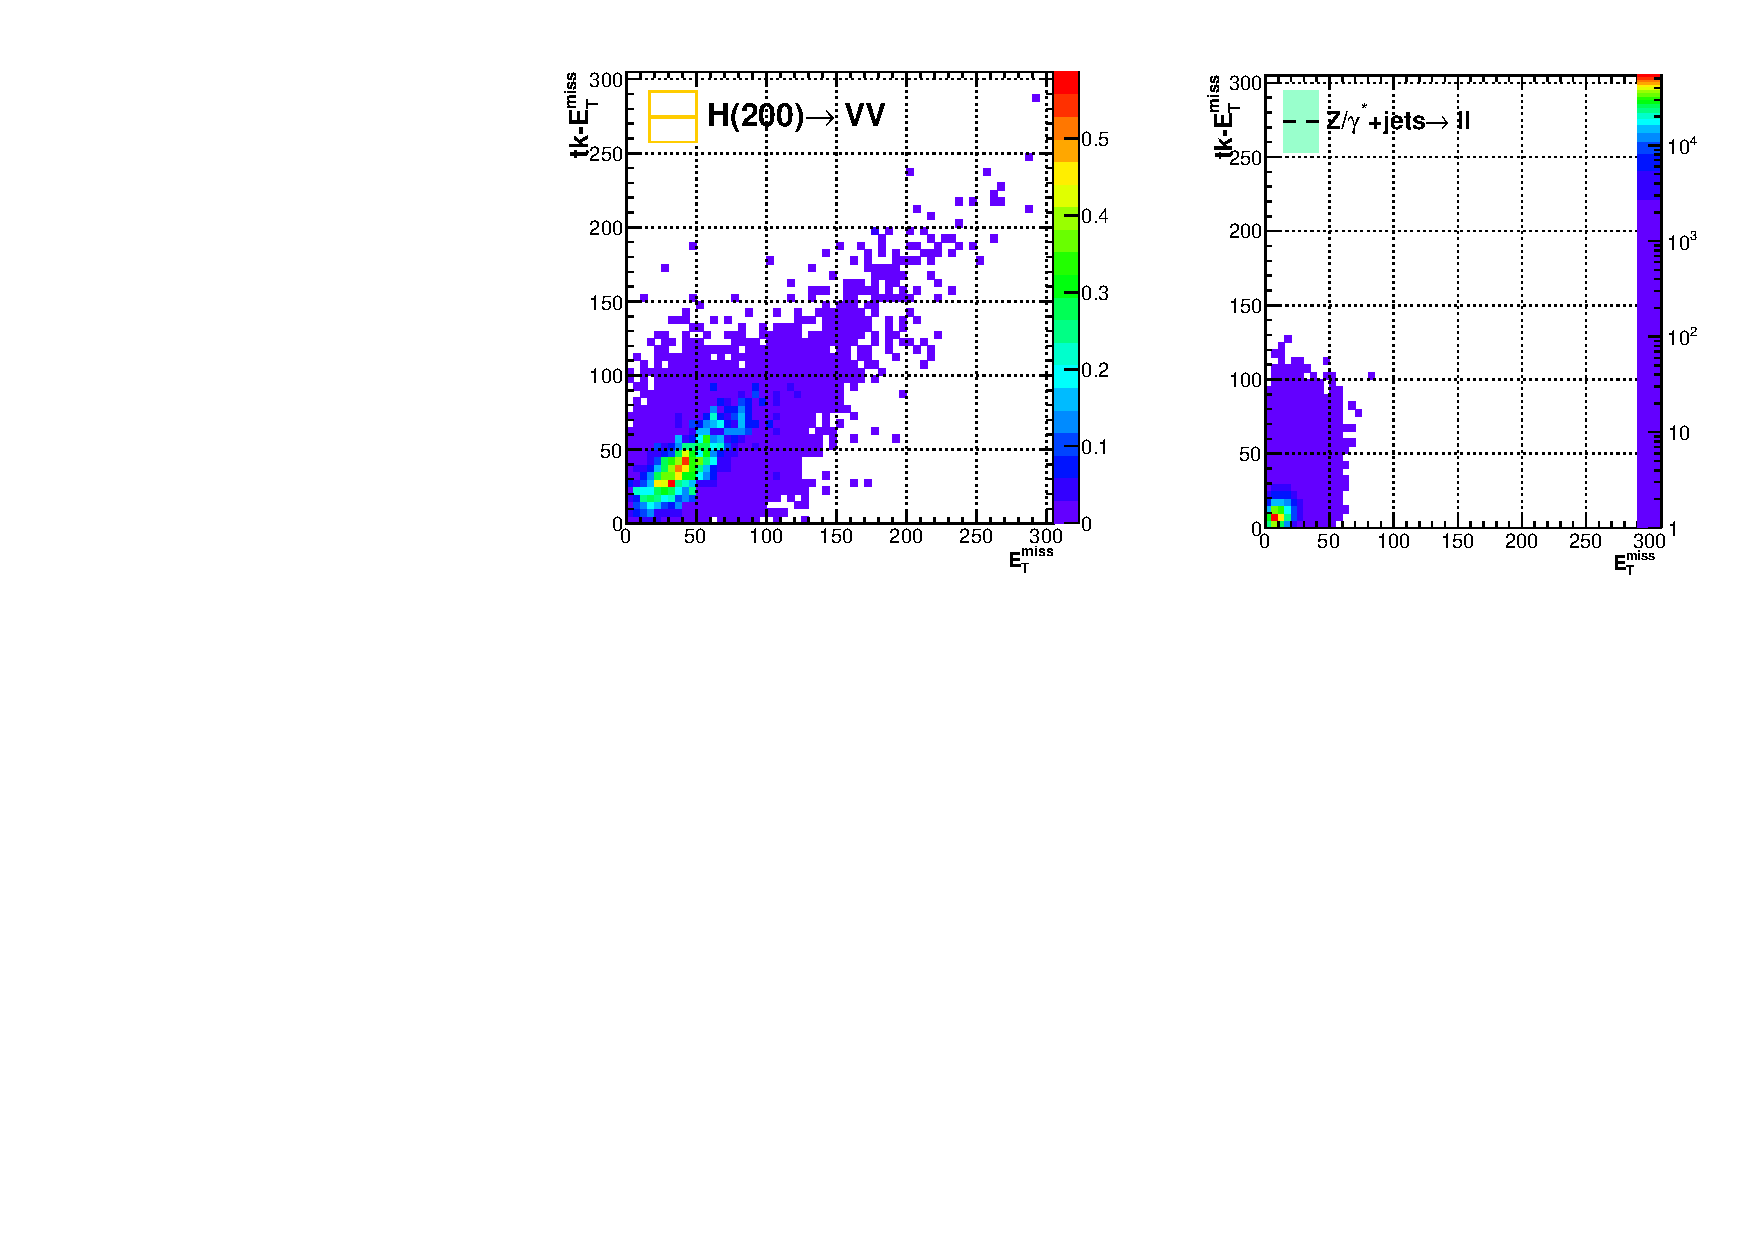
\includegraphics[width=0.9\textwidth]{img/metvstkmet}
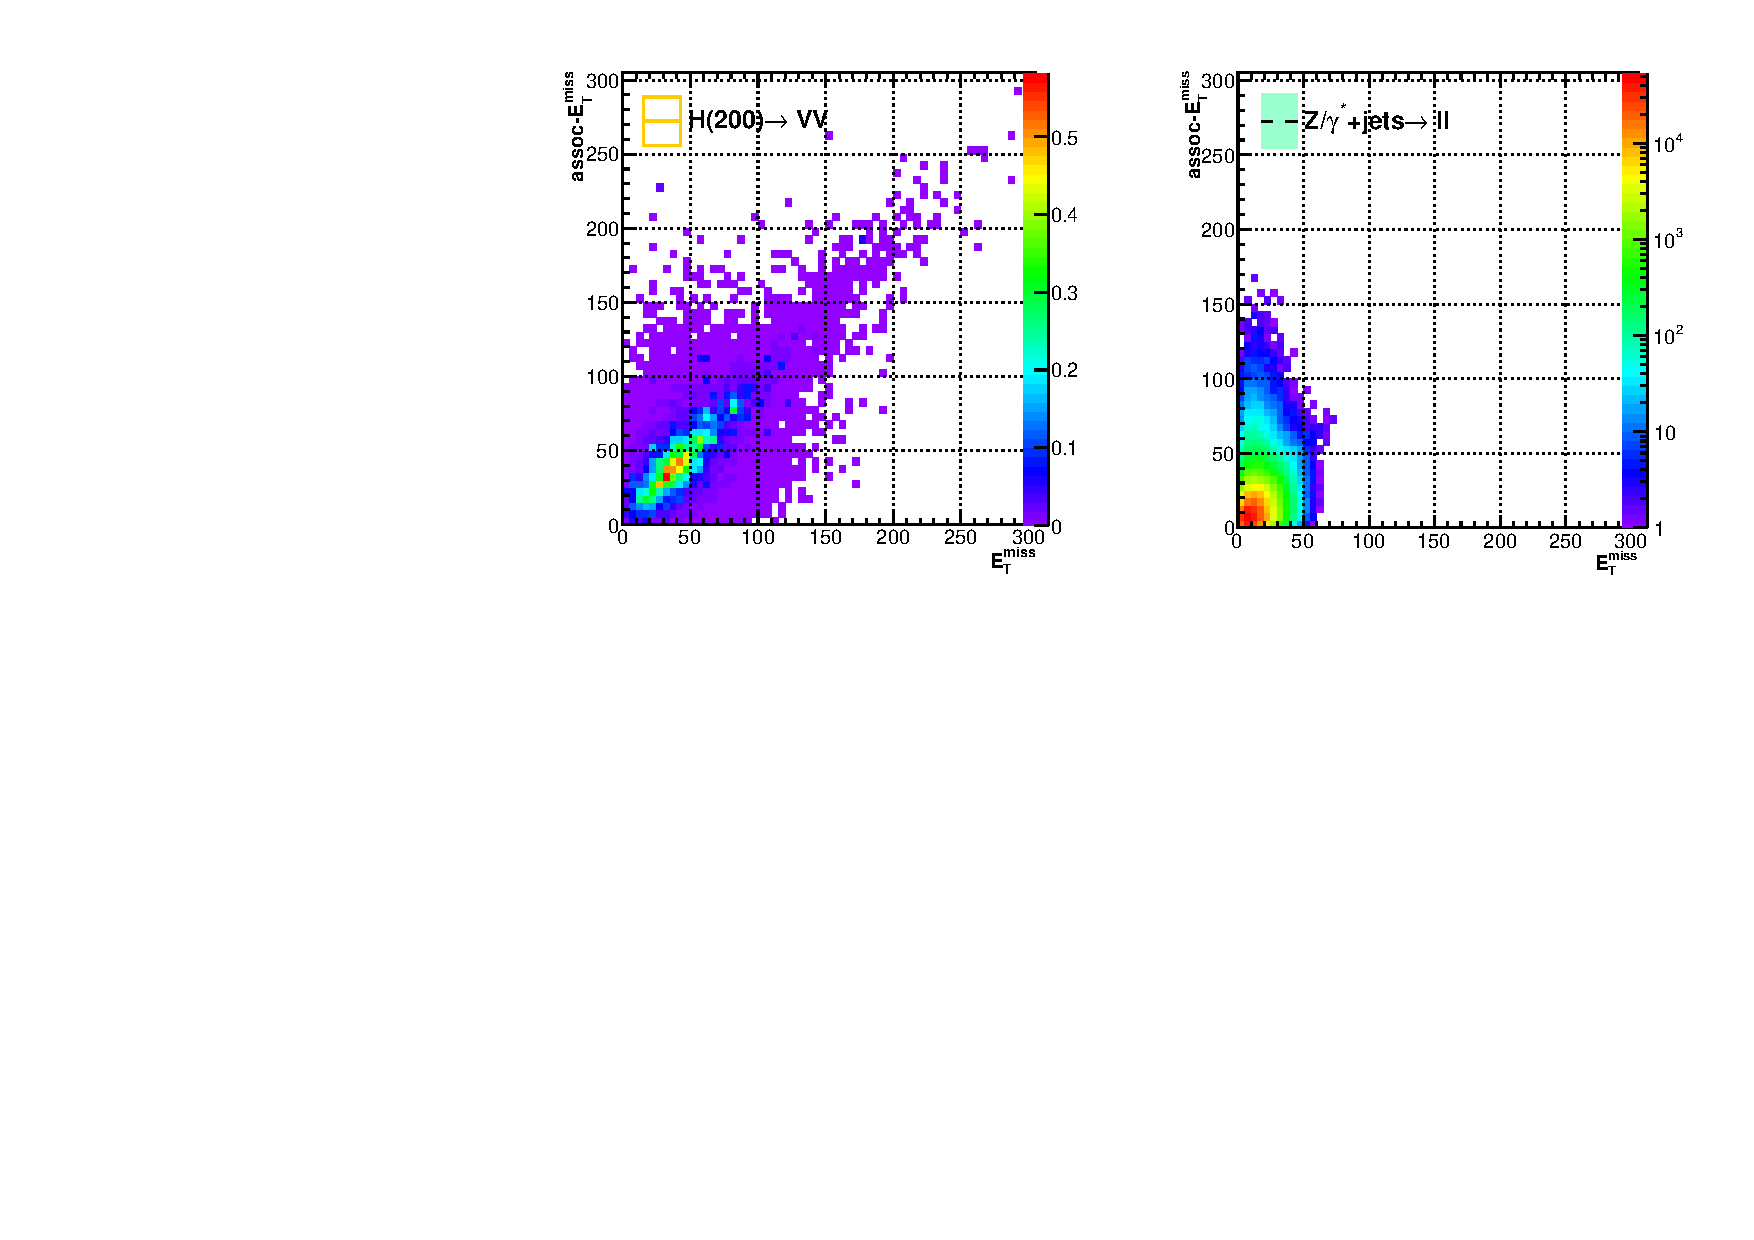
\includegraphics[width=0.9\textwidth]{img/metvsclusteredMet}\\
\caption{Correlation between \MET and \assocChMET ({\em top})
 and between \MET and \assocMET ({\em bottom})
 for a simulated Higgs (m=200~GeV/c$^2$) sample ({\em left}) 
 and a $Z\rightarrow ll$ sample ({\em right}) in the di-muon sample}.
\label{fig:metcorrelations}
\end{center}
\end{figure}


%
%
%
\clearpage
\section{Search for the standard model Higgs in the 2l2$\nu$ final state}
\label{sec:higgssearch}

The next Sections describe three complementary approaches to search for the standard model Higgs in the 2l2$\nu$ final state.
The analysis relies fully on the expected behavior for the Higgs events as described in the simulation.
The transverse momentum of the Higgs boson is however corrected for the NNLO+NNLL 
prediction which are not taken into account by the \Powheg sample used in this study.
The Higgs-$p_T$ reweighting is applied only to gluon-gluon fusion and it is described in more detail in~\cite{CMS-TWIKI-GEN-higgspt}

Two of the analysis proposed are cut-based and a third one is a discriminator based analysis.
For each analysis the events are categorized according to the jet multiplicity observed.
Events with $\geq$2~jets are furthermore analyzed to search for the vector-boson-fusion (VBF) specific signature.
If the event does not meet the VBF specific selection it is accounted for in the $\geq$2~jets bin.

%%
%% Higgs event selection
%%
\subsection{Higgs event selection using a cut-based analysis approach}
\label{subsec:higgsselection}

The selection variables chosen for the search of the Higgs boson production in the gg$\rightarrow$H mode are summarized in Tab.~\ref{tab:gluglucuts}.
The cuts were chosen by maximing the following figure of merit $f=S/\sqrt(S+B)$ after requiring that the instrumental $Z$ background is reduced by a 10$^{-3}$ (medium \RMET working point).
Tor the different mass points signal includes, as in the previous sections, the gluon-gluon and vector boson fusion processes, as well as Higgs decays in both the ZZ and WW channels.
Background includes all the remaining processes after the \RMET cut as listed in Table~\ref{tab:mcsamples}.
The details on the $f$ variable can be found in Sec.~\ref{sec:app:cutbasedoptimization}.
Table~\ref{tab:gluglucuts} summarizes the selection applied as a function of the Higgs mass being searched.

\begin{table}[htp]
\caption{Selection variables for the search for the Higgs boson in the gg$\rightarrow$H mode.}
\label{tab:gluglucuts}
\begin{center}
\begin{tabular}{cccc} \hline\hline
\multirow{2}{*}{Higgs mass (GeV/c$^2$)} & \multicolumn{3}{c}{Variable} \\
                            & $\delta\phi^{ll}$ & \RMET (longitudinal) & $\sum M_T$ \\ \hline
200                         & 1.0$<|x|<$2.75  & $|x|>$50             & $>$150 \\
300                         & $|x|<$2.5         & x$>$75               & $>$200 \\
400                         & $|x|<$2.0         & x$>$75               & $>$300 \\
500                         & $|x|<$2.0         & x$>$100              & $>$400 \\
600                         & $|x|<$1.5         & x$>$150              & $>$400 \\\hline\hline
\end{tabular}
\end{center}
\end{table}

Tables~\ref{tab:gluglucutandcountyields_0jets},
~\ref{tab:gluglucutandcountyields_1jets}
and ~\ref{tab:gluglucutandcountyields_2jets}
summarize the results obtained after applying the selection just described.
An overall good agreement is found between data and direct comparison with MC
for all categories except the 1-jet bin in the $ee$ channel where a slight excess is observed. 
The data-driven estimate of the instrumental and top backgrounds will be discussed in the next sections. 

%%%
\begin{table}[htp]
\caption{Event yields after mass-dependent selection for the di-electron and di-muon channel in events with 0 jets.}
\label{tab:gluglucutandcountyields_0jets}
\begin{center}
\begin{tabular}{cccccc} \hline\hline
{\bf Higgs mass (GeV/c$^2$)}        & {\bf 200}         & {\bf 300}         & {\bf 400}         & {\bf 500}         & {\bf 600}     \\\hline\hline             
                                    &                   &                   &                   &                   &               \\\hline   
\multicolumn{6}{c}{\bf$ee$ channel}\\\hline
S/B expected                        & $0.08 \pm 0.02$   & $0.33 \pm 0.01$   & $0.48 \pm 0.02$   & $0.42 \pm 0.04$   & $0.25 \pm 0.03$  \\\hline   
H$\rightarrow$ VV                   & $ 1.02 \pm0.22 $  & $ 1.83 \pm0.04 $  & $ 1.534 \pm0.034$ & $ 0.56 \pm0.04 $  & $ 0.188 \pm0.004 $ \\\hline
ZZ                                  & $ 4.56 \pm0.14 $  & $ 3.53 \pm0.12 $  & $ 2.30 \pm0.10 $  & $ 1.07 \pm0.07 $  & $ 0.74 \pm0.06 $ \\
WW                                  & $ 3.87 \pm0.34 $  & $ 0.37 \pm0.10 $  & $ 0.09 \pm0.05 $  &  &  \\
WZ                                  & $ 2.73 \pm0.18 $  & $ 1.57 \pm0.14 $  & $ 0.80 \pm0.10 $  & $ 0.25 \pm0.05 $  & $ 0.14 \pm0.04 $ \\
Single top                          & $ 0.08 \pm0.04 $  & $ 0.06 \pm0.04 $  &  &   \\
$t\bar{t}$                          & $ 0.23 \pm0.20 $  &  &  &  &  \\
W+jets                              & $ 0.9 \pm0.9 $    &  &  &  &  \\
Z/$\gamma^{*}$+jets$\rightarrow$ ll & $ 0.54 \pm0.32 $  &  &  &  &  \\\hline
Total expected                      & $ 12.9 \pm1.1 $   & $ 5.53 \pm0.21 $  & $ 3.19 \pm0.15 $  & $ 1.32 \pm0.09 $  & $ 0.87 \pm0.07 $ \\\hline
data                                & $ 16$             & $ 8$              & $ 4$              & $ 2$              &  $ 2$ \\\hline
                                    &                   &                   &                   &                   &               \\\hline   
\multicolumn{6}{c}{\bf$\mu\mu$ channel}\\\hline
S/B expected                        & $0.08 \pm 0.02$   & $0.32\pm0.01$     & $0.48\pm 0.03$      & $0.31\pm 0.03$     &  $0.23\pm 0.02$     \\\hline
H$\rightarrow$ VV                   & $ 1.04 \pm0.21 $  & $ 1.80 \pm0.04 $  & $ 1.460 \pm0.033 $  &$ 0.379 \pm0.032 $  &$ 0.178 \pm0.004 $ \\\hline
ZZ                                  & $ 4.64 \pm0.14 $  & $ 3.62 \pm0.12 $  & $ 2.23 \pm0.10 $    & $ 1.00 \pm0.06 $   & $ 0.62 \pm0.05 $ \\
WW                                  & $ 4.7 \pm0.4 $    & $ 0.54 \pm0.12 $  & $ 0.10 \pm0.06 $    &                    & \\
WZ                                  & $ 2.72 \pm0.18 $  & $ 1.33 \pm0.13 $  & $ 0.67 \pm0.09 $    & $ 0.24 \pm0.05 $   & $ 0.15 \pm0.04 $ \\
Single top                          & $ 0.29 \pm0.09 $  & $ 0.07 \pm0.05 $  & $ 0.04 \pm0.04 $    &                    & \\
$t\bar{t}$                          & $ 0.06 \pm0.06 $  &                   &                     &                    & \\
W+jets                              &                   &                   &                     &                    & \\
Z/$\gamma^{*}$+jets$\rightarrow$ ll & $ 0.7 \pm0.4 $    &                   &                     &                    &  \\\hline
Total expected                      & $ 13.1 \pm0.6 $   & $ 5.56 \pm0.22 $  & $ 3.04 \pm0.15 $    & $ 1.24 \pm0.08 $   & $ 0.77 \pm0.06 $ \\\hline
data                                & $ 13 $            & $ 6$              & $ 2$                & $ 2 $              & $ 2 $ \\\hline
\end{tabular}
\end{center}
\end{table}

%%%
\begin{table}[htp]
\caption{Event yields after mass-dependent selection for the di-electron and di-muon channel in events with 1 jet.}
\label{tab:gluglucutandcountyields_1jets}
\begin{center}
\hspace*{-1cm}
\begin{tabular}{cccccc} \hline\hline
{\bf Higgs mass (GeV/c$^2$)}        & {\bf 200}         & {\bf 300}         & {\bf 400}         & {\bf 500}         & {\bf 600}     \\\hline\hline             
                                    &                   &                   &                   &                   &               \\\hline   
\multicolumn{6}{c}{\bf$ee$ channel}\\\hline
S/B expected                        & $0.06 \pm 0.01$   & $0.30 \pm 0.03$   & $0.51 \pm 0.07$   & $0.65 \pm 0.06$   & $0.38 \pm 0.04$  \\\hline   
H$\rightarrow$ VV                   & $ 0.79 \pm0.16 $  & $ 1.90 \pm0.04 $    & $ 1.87 \pm0.04 $  & $ 0.75 \pm0.04 $  & $ 0.282 \pm0.005 $ \\\hline
ZZ                                  & $ 2.91 \pm0.11 $  & $ 2.43 \pm0.10 $  & $ 1.60 \pm0.08 $  & $ 0.77 \pm0.06 $  & $ 0.49 \pm0.05 $ \\
WW                                  & $ 2.15 \pm0.24 $  & $ 0.29 \pm0.09 $  & $ 0.04 \pm0.04 $  & $ ( 1.6 \pm1.6 ) \times10^{-3} $  & $ ( 1.6 \pm1.6 ) \times10^{-3} $ \\
WZ                                  & $ 2.67 \pm0.18 $  & $ 1.84 \pm0.15 $  & $ 1.10 \pm0.12 $  & $ 0.39 \pm0.07 $  & $ 0.25 \pm0.05 $ \\
Single top                          & $ 0.64 \pm0.14 $  & $ 0.19 \pm0.08 $  & $ 0.039 \pm0.034 $  &  &  \\
$t\bar{t}$                          & $ 1.2 \pm0.4 $    & $ 0.34 \pm0.24 $  &                     &  & \\
W+jets                              & $ 0.19 \pm0.19 $  &                   &                     &  &  \\
Z/$\gamma^{*}$+jets$\rightarrow$ ll & $ 2.9 \pm0.9 $    & $ 1.2 \pm0.6 $    & $ 0.9 \pm0.5 $      &  & \\\hline
Total expected                      & $ 12.6 \pm1.1 $   & $ 6.3 \pm0.6 $    & $ 3.7 \pm0.5 $      & $ 1.16 \pm0.09 $  & $ 0.74 \pm0.07 $ \\\hline
data                                & $ 21$             & $ 11$             & $ 6$                & $ 2$    & \\\hline
                                    &                   &                   &                     &                   &               \\\hline   
\multicolumn{6}{c}{\bf$\mu\mu$ channel}\\\hline
S/B expected                        & $0.08 \pm 0.02$   & $0.31\pm0.03$     & $0.57\pm 0.07$      & $0.62\pm 0.06$     &  $0.37\pm 0.03$     \\\hline   
H$\rightarrow$ VV                   & $ 1.13 \pm0.20 $  & $ 1.89 \pm0.04 $  & $ 1.759 \pm0.035 $  & $ 0.66 \pm0.04 $   & $ 0.255 \pm0.005 $ \\\hline
ZZ                                  & $ 3.07 \pm0.11 $  & $ 2.43 \pm0.10 $  & $ 1.63 \pm0.08 $    & $ 0.74 \pm0.05 $   & $ 0.54 \pm0.05 $ \\
WW                                  & $ 2.47 \pm0.27 $  & $ 0.31 \pm0.10 $  &                     &                    & \\ 
WZ                                  & $ 2.92 \pm0.19 $  & $ 1.47 \pm0.13 $  & $ 0.91 \pm0.11 $    & $ 0.32 \pm0.06 $   & $ 0.15 \pm0.04 $ \\
Single top                          & $ 0.76 \pm0.16 $  & $ 0.21 \pm0.08 $  & $ 0.04 \pm0.04 $    &                    & \\
$t\bar{t}$                          & $ 1.0 \pm0.4 $    & $ 0.78 \pm0.34 $  &                     &                    & \\
W+jets                              &                   &                   &                     &                    & \\
Z/$\gamma^{*}$+jets$\rightarrow$ ll & $ 3.5 \pm1.0 $    & $ 0.9 \pm0.5 $    & $ 0.6 \pm0.4 $      &                    & \\\hline
Total expected                      & $ 13.8 \pm1.2 $   & $ 6.1 \pm0.6 $    & $ 3.1 \pm0.4 $      & $ 1.06 \pm0.08 $   & $ 0.69 \pm0.06 $ \\\hline
data                                & $ 12$             & $ 4 $             & $ 2$                & $ 1$               & $ 1$ \\\hline
\end{tabular}
\end{center}
\end{table}

%%%%
\begin{table}[htp]
\caption{Event yields after mass-dependent selection for the di-electron and di-muon channel in events with at least 2 jets.}
\label{tab:gluglucutandcountyields_2jets}
\begin{center}
\begin{tabular}{cccccc} \hline\hline
{\bf Higgs mass (GeV/c$^2$)}        & {\bf 200}         & {\bf 300}         & {\bf 400}         & {\bf 500}         & {\bf 600}     \\\hline\hline             
                                    &                   &                   &                   &                   &               \\\hline   
\multicolumn{6}{c}{\bf$ee$ channel}\\\hline
S/B expected                        & $0.06 \pm 0.01$   & $0.22 \pm 0.03$   & $0.45 \pm 0.08$     & $0.70 \pm 0.12$     & $0.66 \pm 0.09$  \\\hline   
H$\rightarrow$ VV                   & $ 0.98 \pm0.20 $  & $ 1.46 \pm0.04 $  & $ 1.812 \pm0.035 $  & $ 0.81 \pm0.05 $    & $ 0.349 \pm0.006 $\\\hline
ZZ                                  & $ 1.44 \pm0.08 $  & $ 1.16 \pm0.07 $  & $ 0.84 \pm0.06 $    & $ 0.43 \pm0.04 $    & $ 0.265 \pm0.033 $ \\
WW                                  & $ 1.36 \pm0.20 $  & $ 0.33 \pm0.10 $  & $ 0.026 \pm0.020 $  & $ 0.007 \pm0.007 $  & $ 0.007 \pm0.007 $ \\
WZ                                  & $ 1.79 \pm0.15 $  & $ 1.18 \pm0.12 $  & $ 0.89 \pm0.10 $    & $ 0.47 \pm0.08 $    & $ 0.26 \pm0.06 $ \\
Single top                          & $ 1.13 \pm0.20 $  & $ 0.26 \pm0.09 $  & $ 0.034 \pm0.034 $  &  & \\
$t\bar{t}$                          & $ 5.5 \pm0.9 $    & $ 2.0 \pm0.5 $    & $ 0.55 \pm0.26 $    &  & \\
W+jets                              &  &  &  &  &  \\
Z/$\gamma^{*}$+jets$\rightarrow$ ll & $ 6.0 \pm1.2 $    & $ 1.7 \pm0.6 $    & $ 1.6 \pm0.6 $     & $ 0.24 \pm0.17 $  & \\\hline
Total expected                      & $ 17.2 \pm1.6 $   & $ 6.6 \pm0.9 $    & $ 4.0 \pm0.7 $     & $ 1.15 \pm0.19 $  & $ 0.53 \pm0.07 $ \\\hline
data                                & $ 22$             & $ 10.0$           & $ 4.0$             & $ 1.0$            & \\\hline
                                    &                   &                   &                    &                   &               \\\hline   
\multicolumn{6}{c}{\bf$\mu\mu$ channel}\\\hline
S/B expected                        & $0.03 \pm 0.01$   & $0.18\pm0.03$     & $0.32\pm 0.06$      & $0.27\pm 0.08$     &  $0.25\pm 0.10$     \\\hline   
H$\rightarrow$ VV                   & $ 0.58 \pm0.12 $  & $ 1.49 \pm0.04 $  & $ 1.766 \pm0.034 $  & $0.78 \pm0.05 $    & $ 0.297 \pm0.005 $ \\\hline
ZZ                                  & $ 1.40 \pm0.07 $  & $ 1.17 \pm0.07 $  & $ 0.78 \pm0.05 $    & $ 0.39 \pm0.04 $   & $ 0.234 \pm0.030 $ \\
WW                                  & $ 1.36 \pm0.20 $  & $ 0.17 \pm0.07 $  &                     &                    & \\
WZ                                  & $ 1.85 \pm0.15 $  & $ 1.17 \pm0.12 $  & $ 0.76 \pm0.10 $    & $ 0.36 \pm0.07 $   & $ 0.16 \pm0.04 $ \\
Single top                          & $ 0.96 \pm0.16 $  & $ 0.19 \pm0.08 $  &                     &                    &\\
$t\bar{t}$                          & $ 5.0 \pm0.8 $    & $ 1.3 \pm0.4 $    & $ 0.05 \pm0.05 $    &                    & \\
W+jets                              &  &  &  &  &  \\
Z/$\gamma^{*}$+jets$\rightarrow$ ll & $ 8.6 \pm1.5 $    & $ 4.4 \pm1.1 $    & $ 4.0 \pm1.1 $      & $ 2.2 \pm0.8 $  & $ 0.8 \pm0.5 $ \\\hline
Total expected                      & $ 19.1 \pm1.8 $   & $ 8.4 \pm1.2 $    & $ 5.5 \pm1.1 $      & $ 2.9 \pm0.8 $  & $ 1.2 \pm0.5 $ \\ \hline
data                                & $ 22$             & $ 7 $             & $ 6 $               & $ 1$            & \\\hline
\end{tabular}
\end{center}
\end{table}

%%
%% Discriminator analysis
%%
\subsection{Discriminator based analysis of the selected events}
\label{subsec:discanalysis}

Tables~\ref{tab:gluglucutandcountyields_0jets},~\ref{tab:gluglucutandcountyields_1jets},~\ref{tab:gluglucutandcountyields_2jets}
show the expected number of events surviving the \RMET selection.
In the low jet multiplicity bins di-boson processes are are the dominant remaining backgrounds.
For events with at least two jets residual \ttbar and DY are expected to survive the medium working point selection 
but to be negligigible in the high mass selection region.

To further enhance the signal to backround ratio we setup a multivariate analysis exploiting mainly angular variables for the
rejection of the irreducible di-boson processes. The analysis is implemented using the TMVA package~\cite{Hocker:2007ht}.

In the current implementation the variables used for the selection are:

\begin{description}

\item[$\Delta \phi (lead-\ell, \ell\ell)$]: azimuthal angle between the leading lepton and the di-lepton system;

\item[$\Delta R (\ell, \ell)$]: phase-space distance between the two leptons;

\item[$\sum M_T$]: sum of the individual transverse masses of each lepton and \MET. For each lepton the individual transverse mass is computed as:

\begin{equation}
M_T(\ell,E_T^{miss})=2p_T^{\ell}E_T^{miss}(1-\cos\delta\phi)
\label{eq:transversemass}
\end{equation}

where $\delta\phi$ is the azimuthal angle between the lepton and the \MET directions.

\item[\RMET (longitudinal)]: projection of the \RMET variable in the longitudinal direction (cf. Sec.~\ref{subsec:redmet})

\end{description}

Figure~\ref{fig:angles} shows schematically the angular observables used to implement the discriminant.

\begin{figure}[htp]
\begin{center}
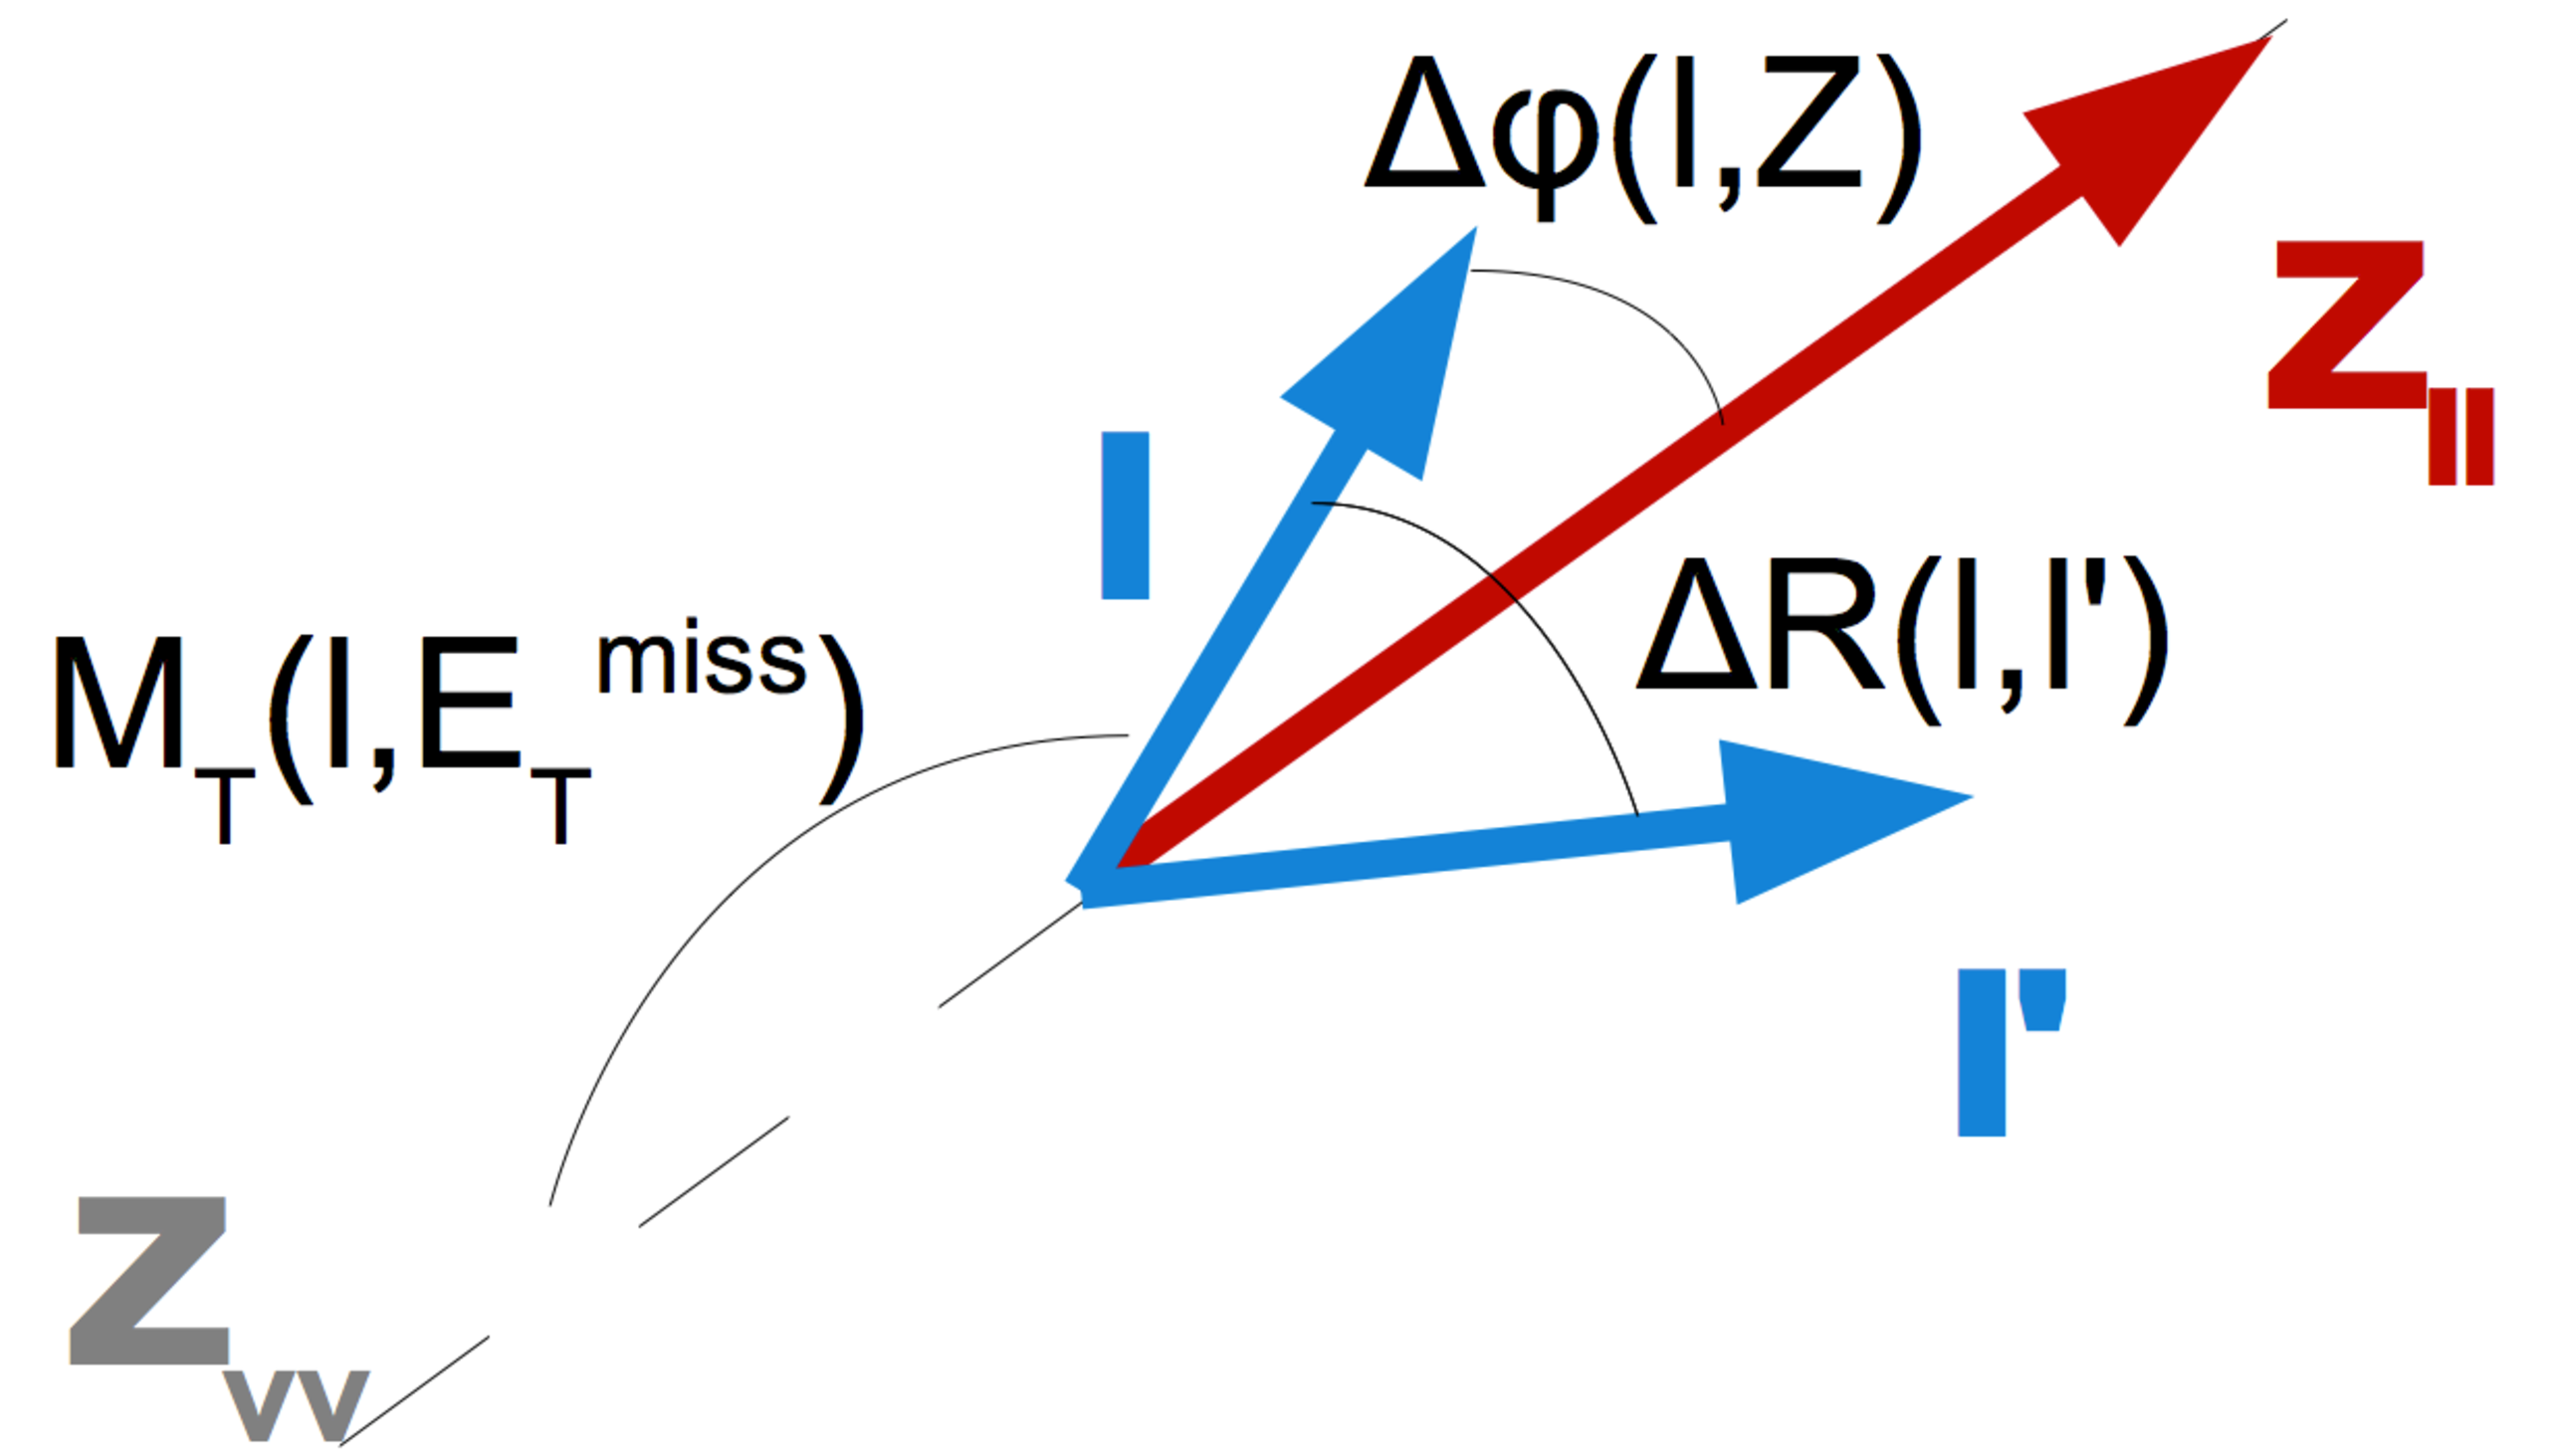
\includegraphics[width=0.35\textwidth]{img/angles}
\caption{Angular variables used in the implementation of the multivariate discriminant.}
\label{fig:angles}
\end{center}
\end{figure}

The distribution of the angular variables for all the backgrounds and
for the different mass hipothesis for the signal 
are shown after the medium \RMET cut in Figure~\ref{fig:input_redMET}.
Overall the level of agreement between data and Monte-Carlo can be
considered satisfactory for all the variables.

\begin{figure}[htp]
\begin{center}
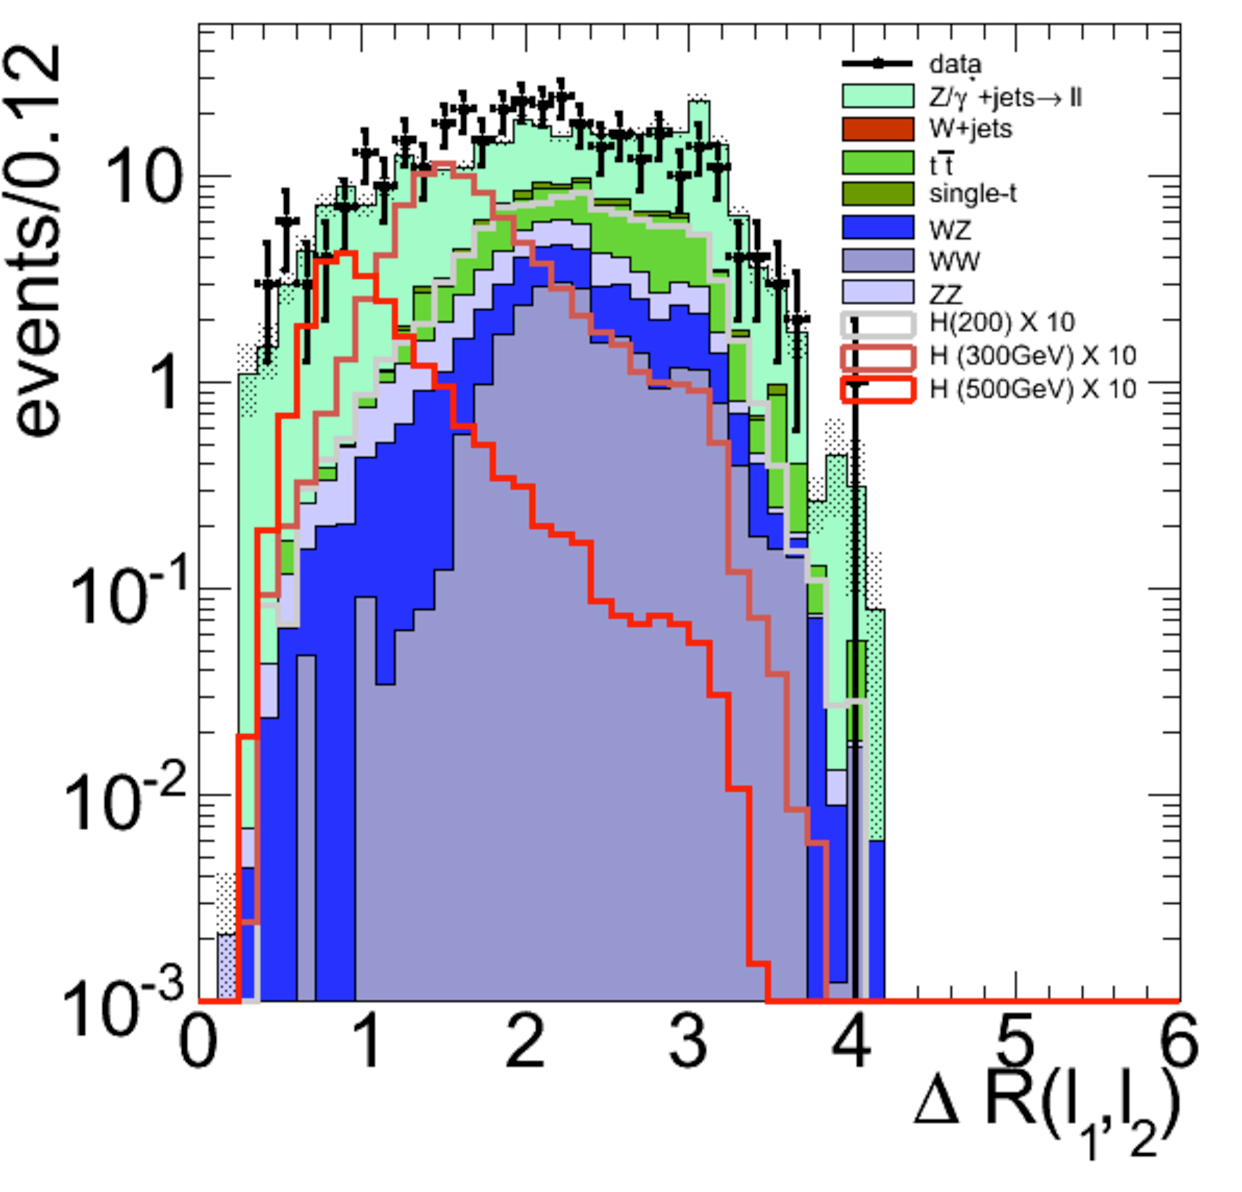
\includegraphics[width=0.3\textwidth]{img/cStack_deltaRLept_mumu_lveto_nob_redmetL}
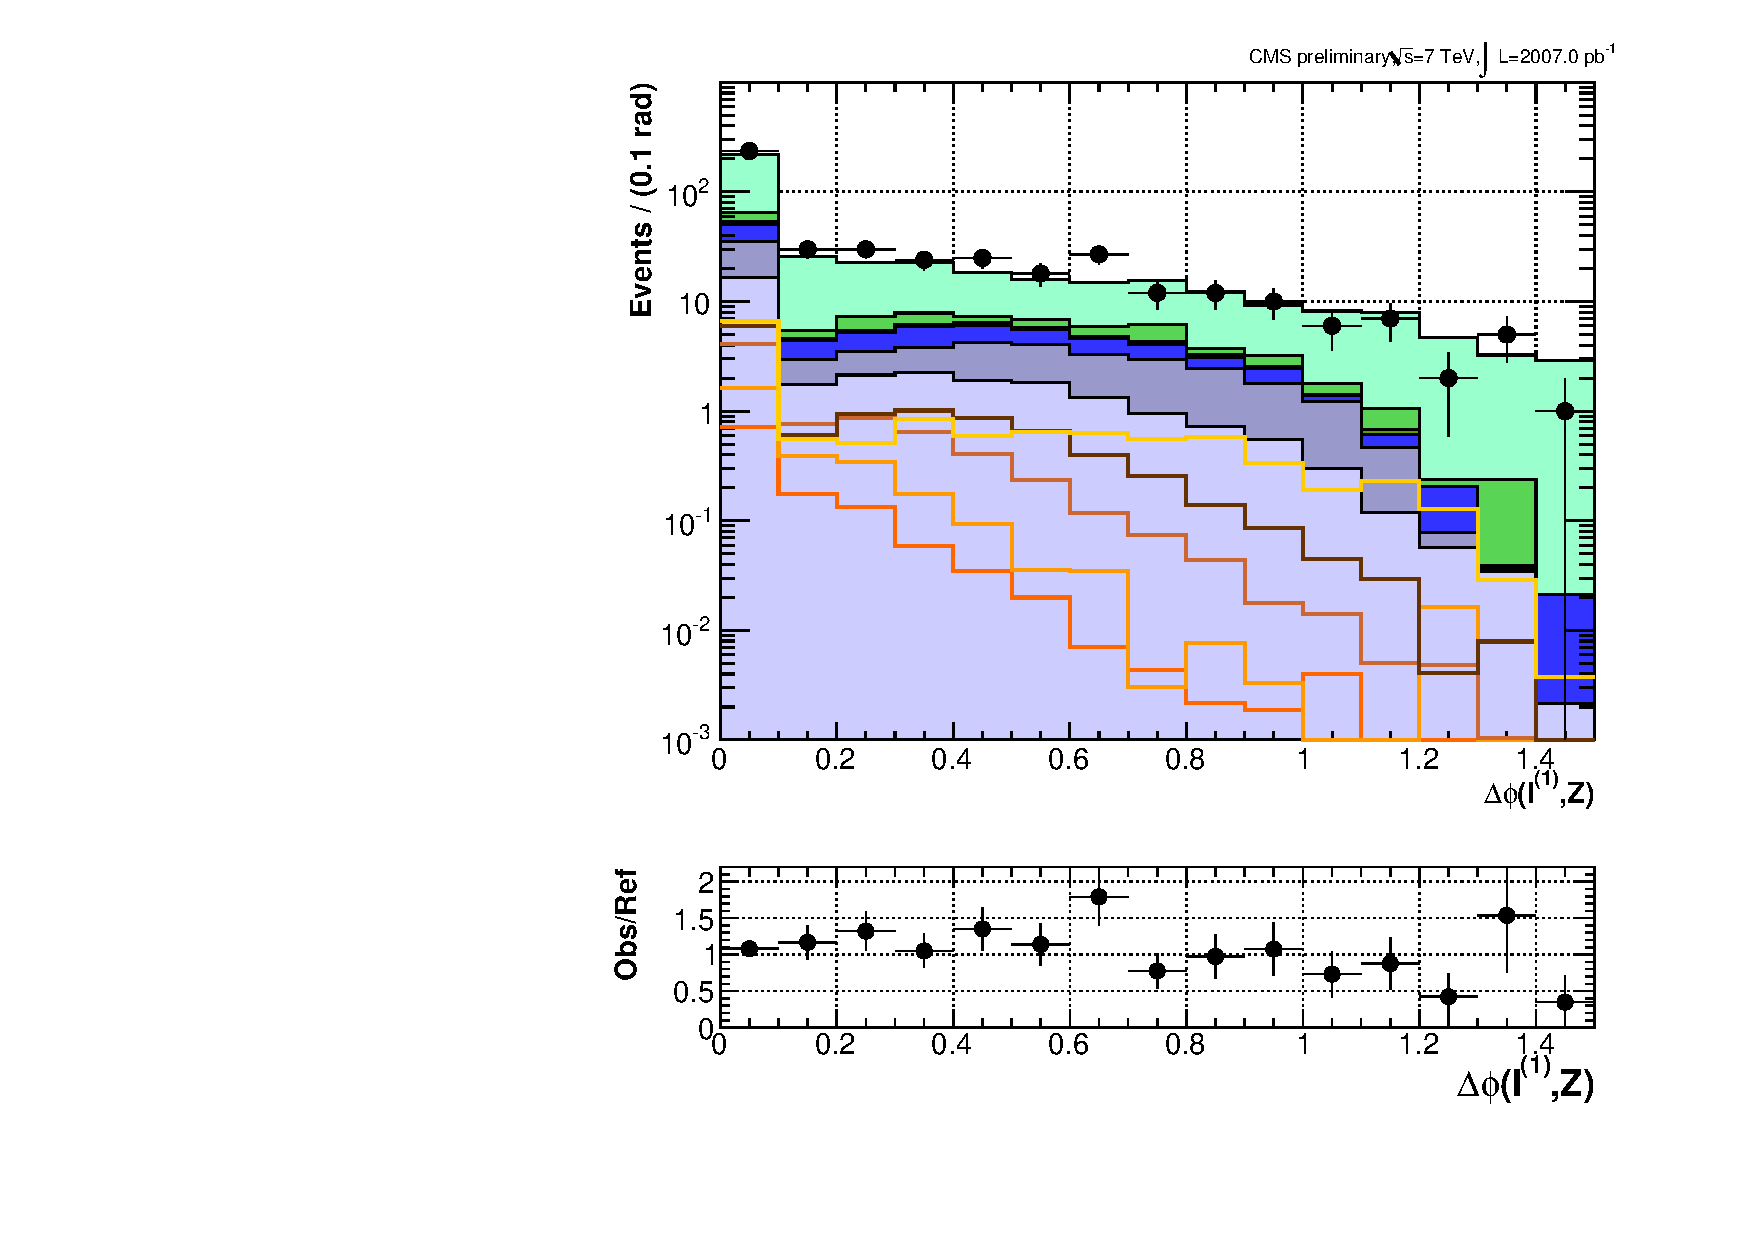
\includegraphics[width=0.3\textwidth]{img/cStack_deltaPhiLeadZ_mumu_lveto_nob_redmetL}
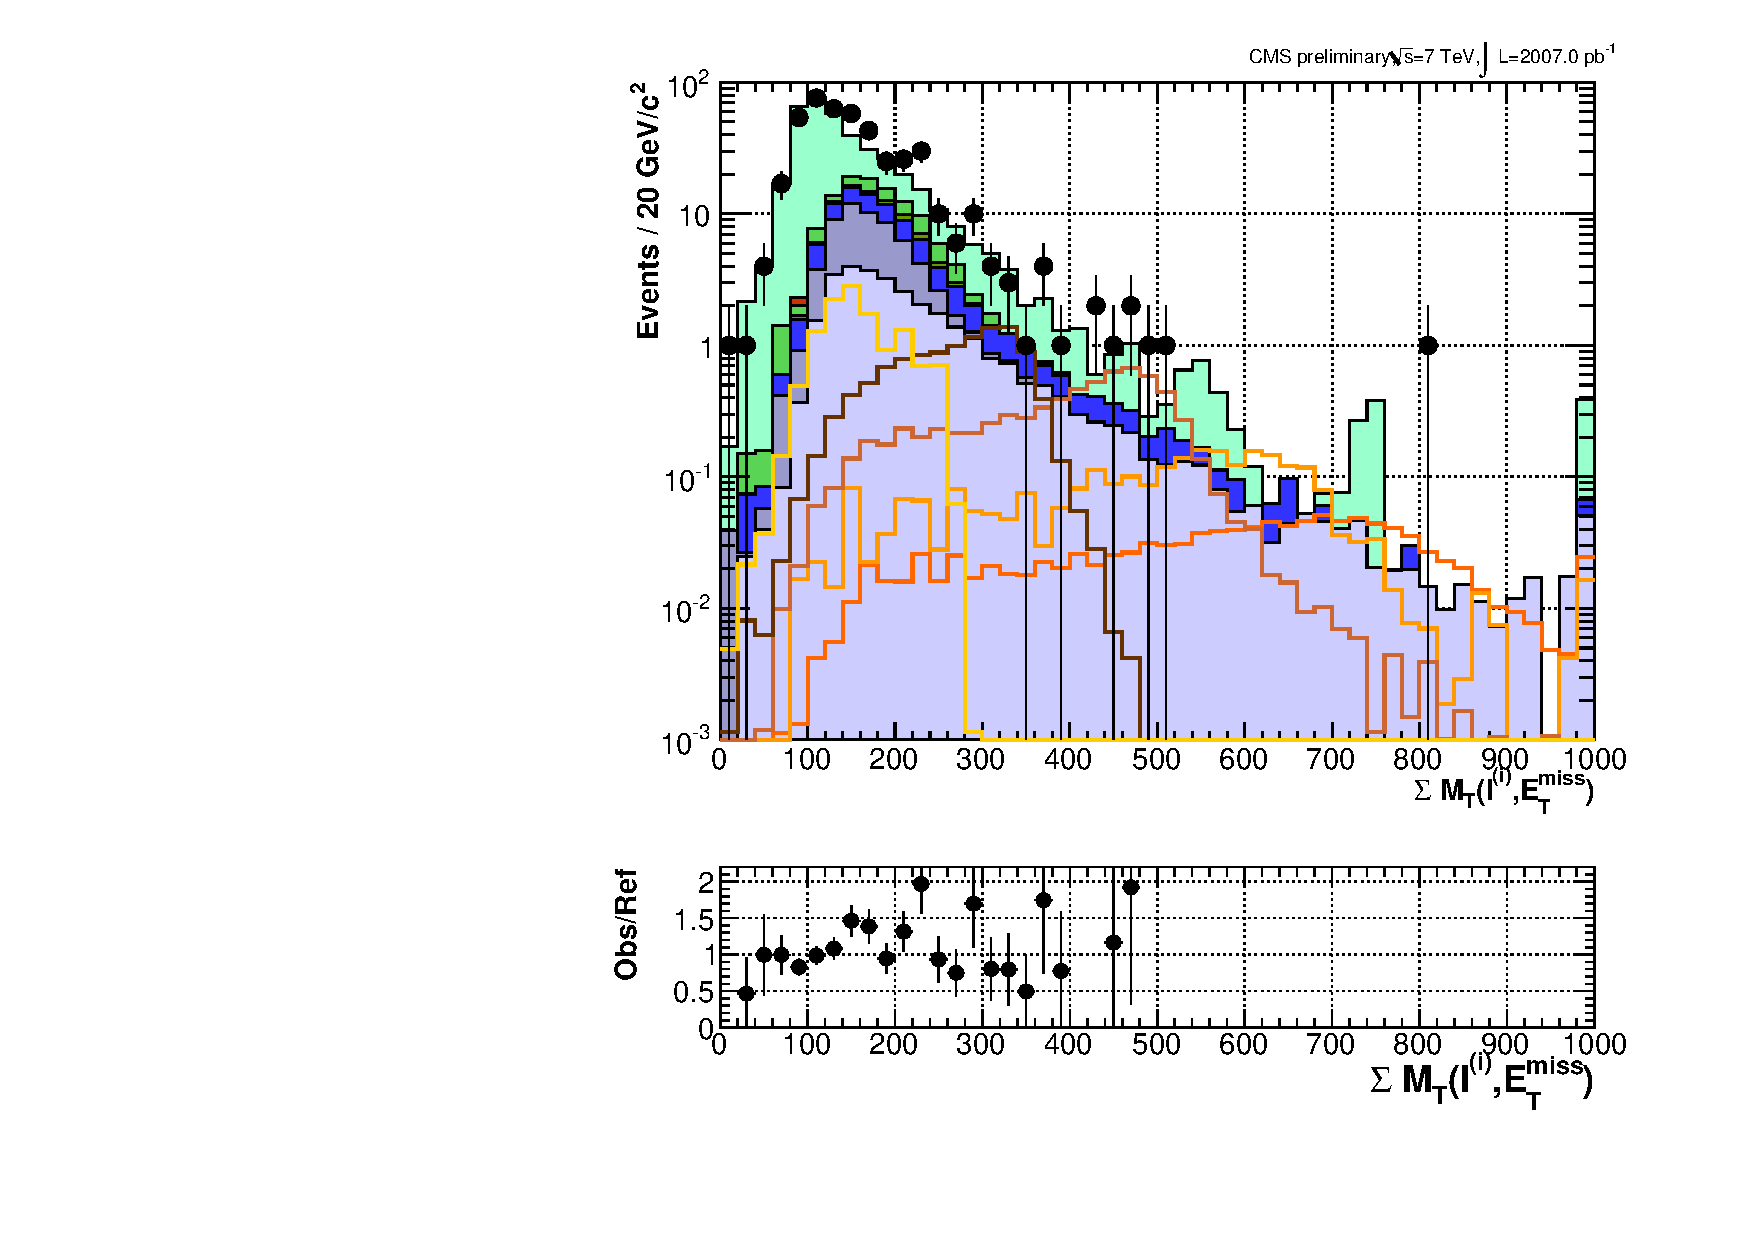
\includegraphics[width=0.3\textwidth]{img/cStack_mtSumLMet_mumu_lveto_nob_redmetL}\\
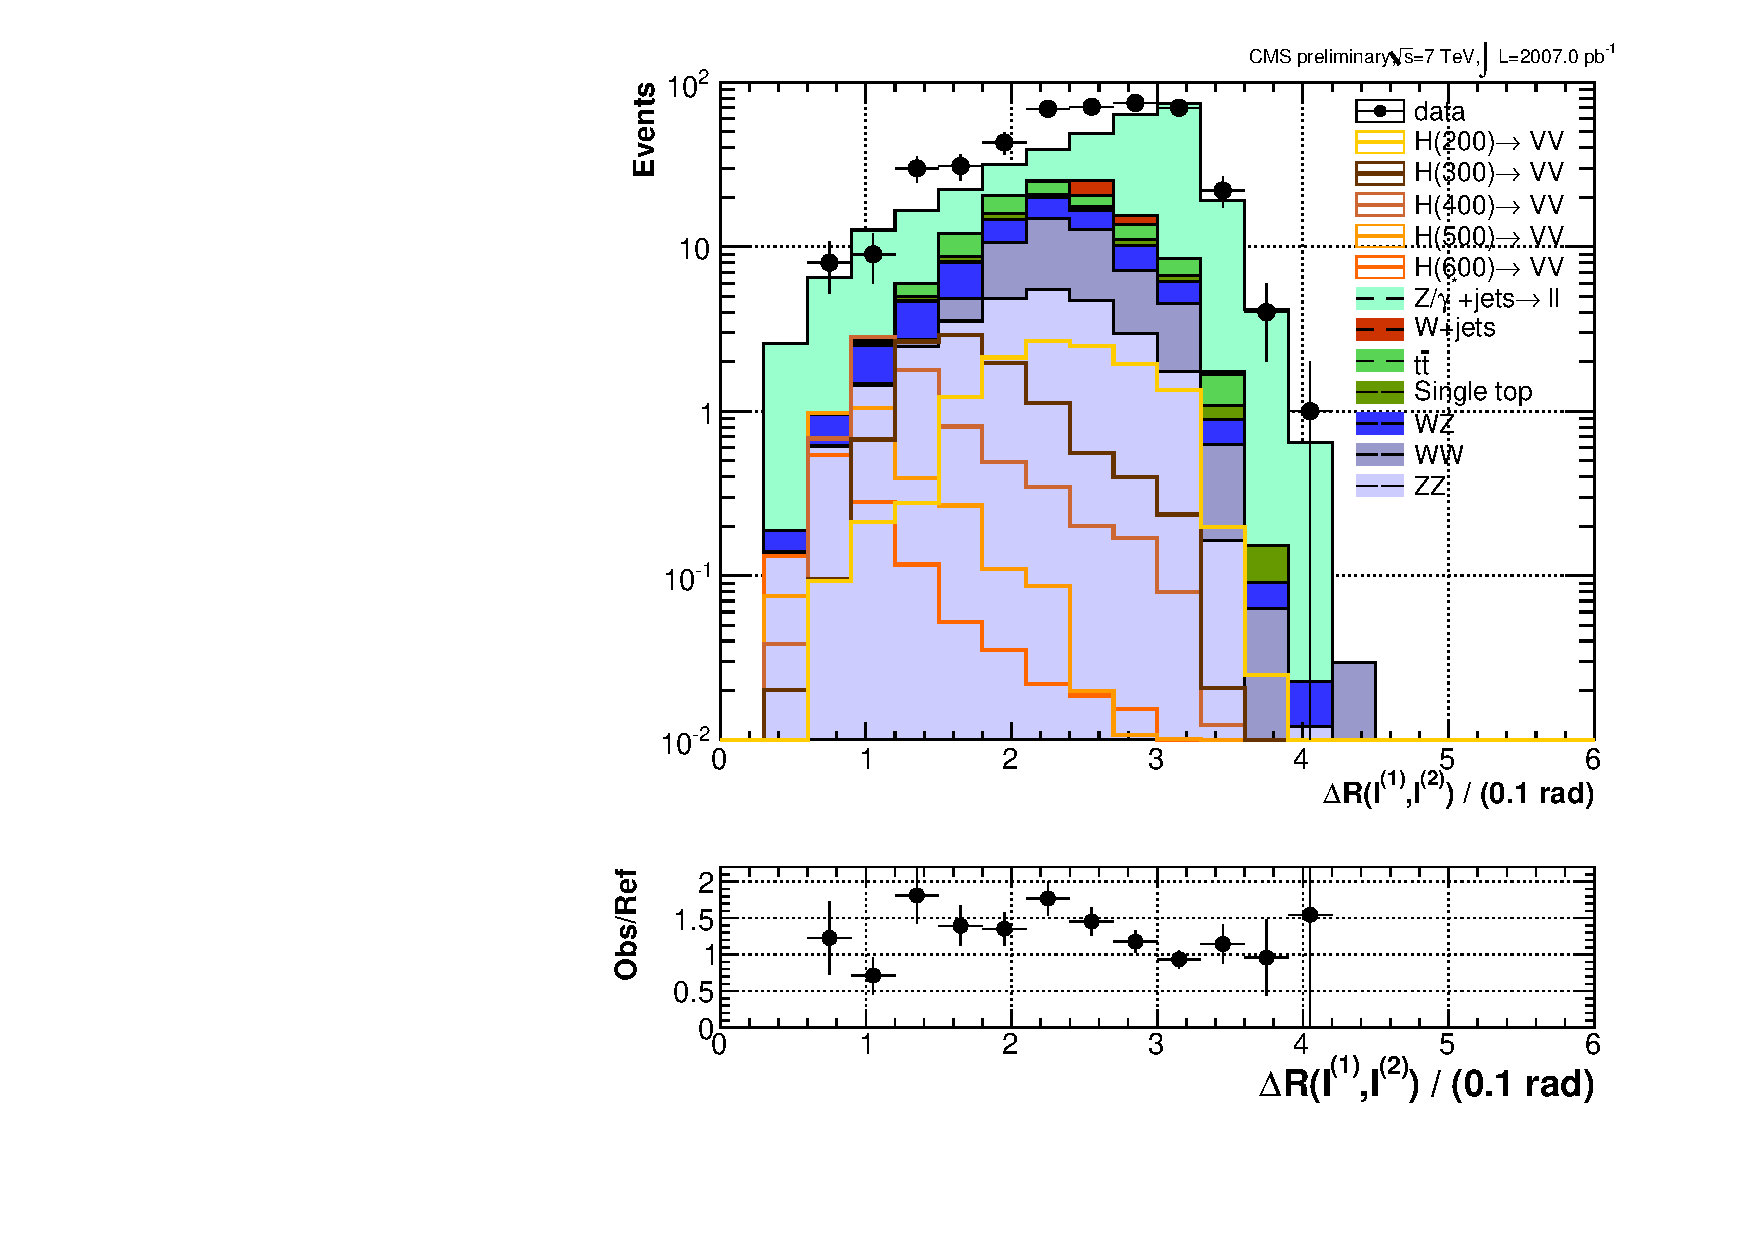
\includegraphics[width=0.3\textwidth]{img/cStack_deltaRLept_ee_lveto_nob_redmetL}
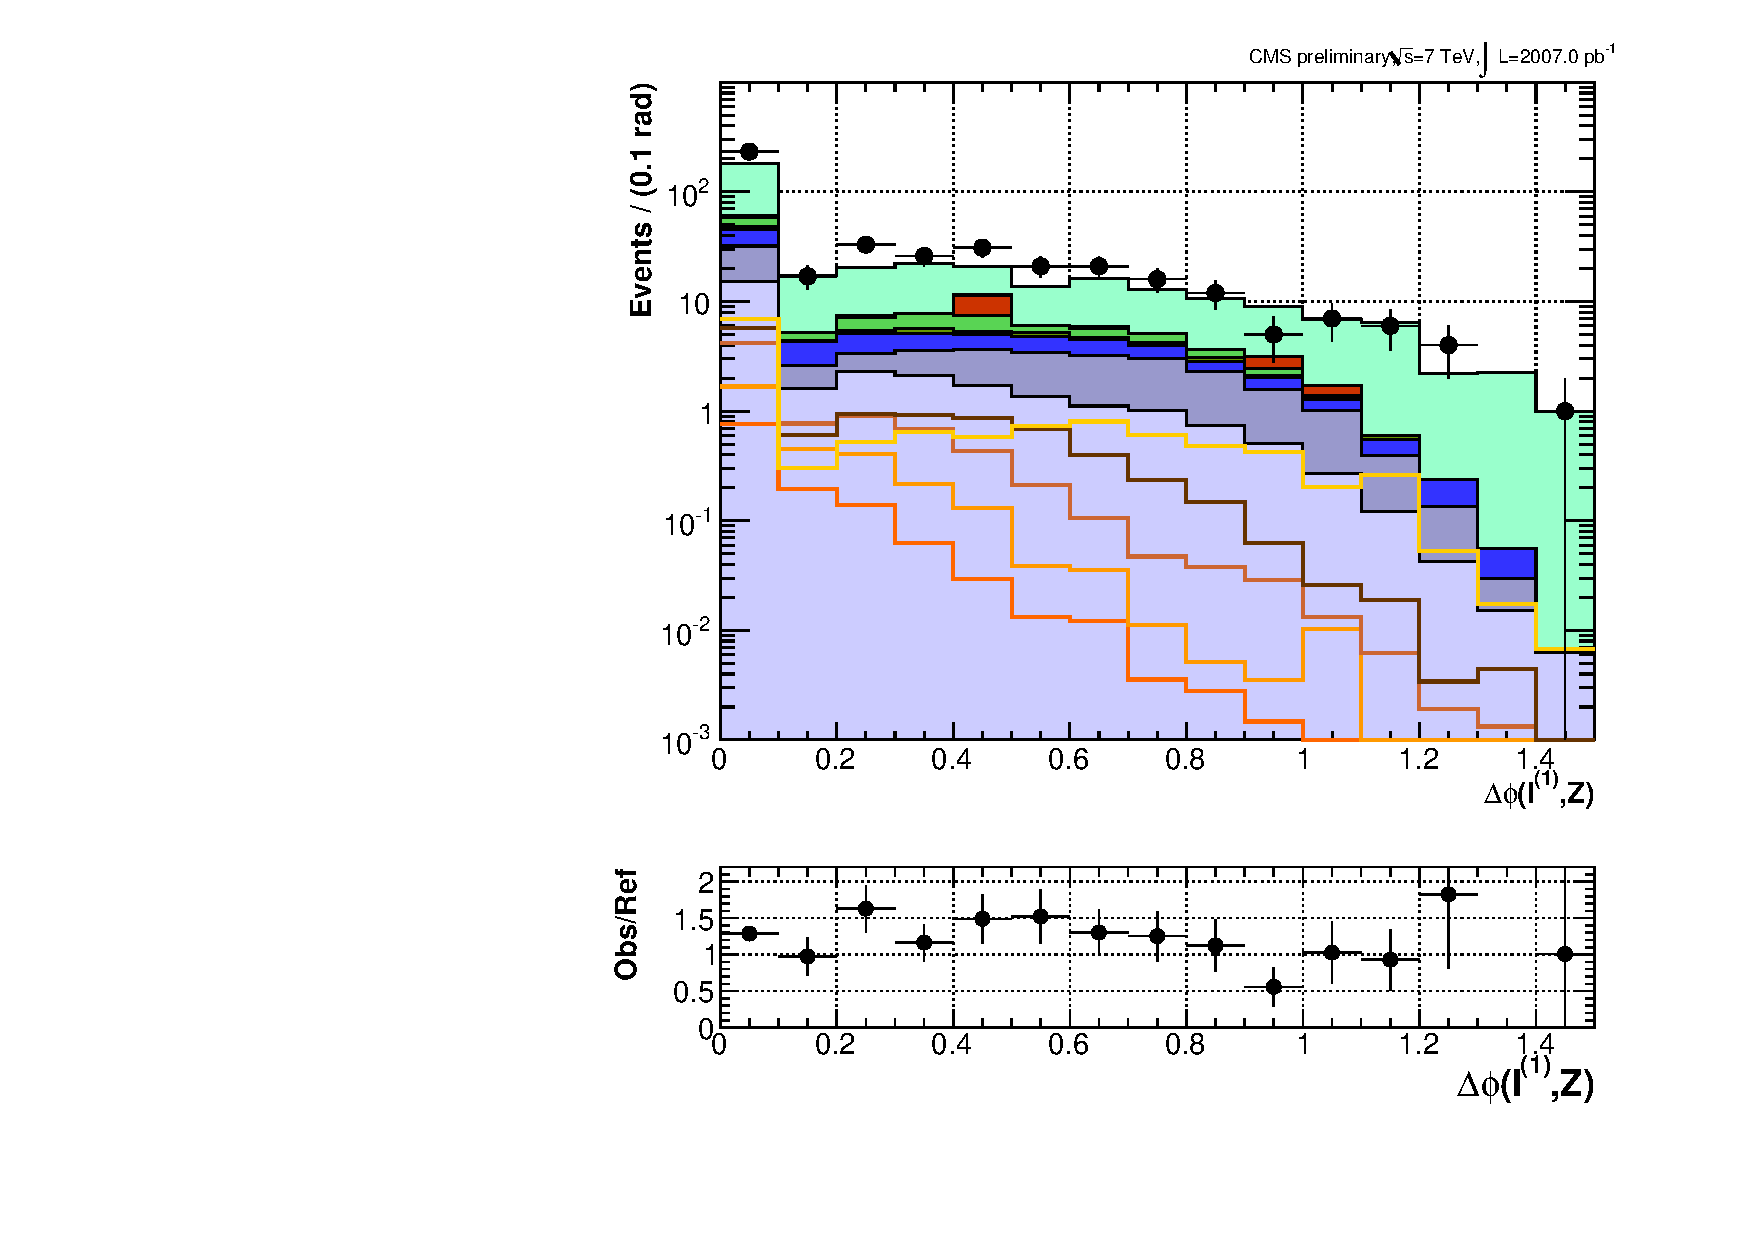
\includegraphics[width=0.3\textwidth]{img/cStack_deltaPhiLeadZ_ee_lveto_nob_redmetL}
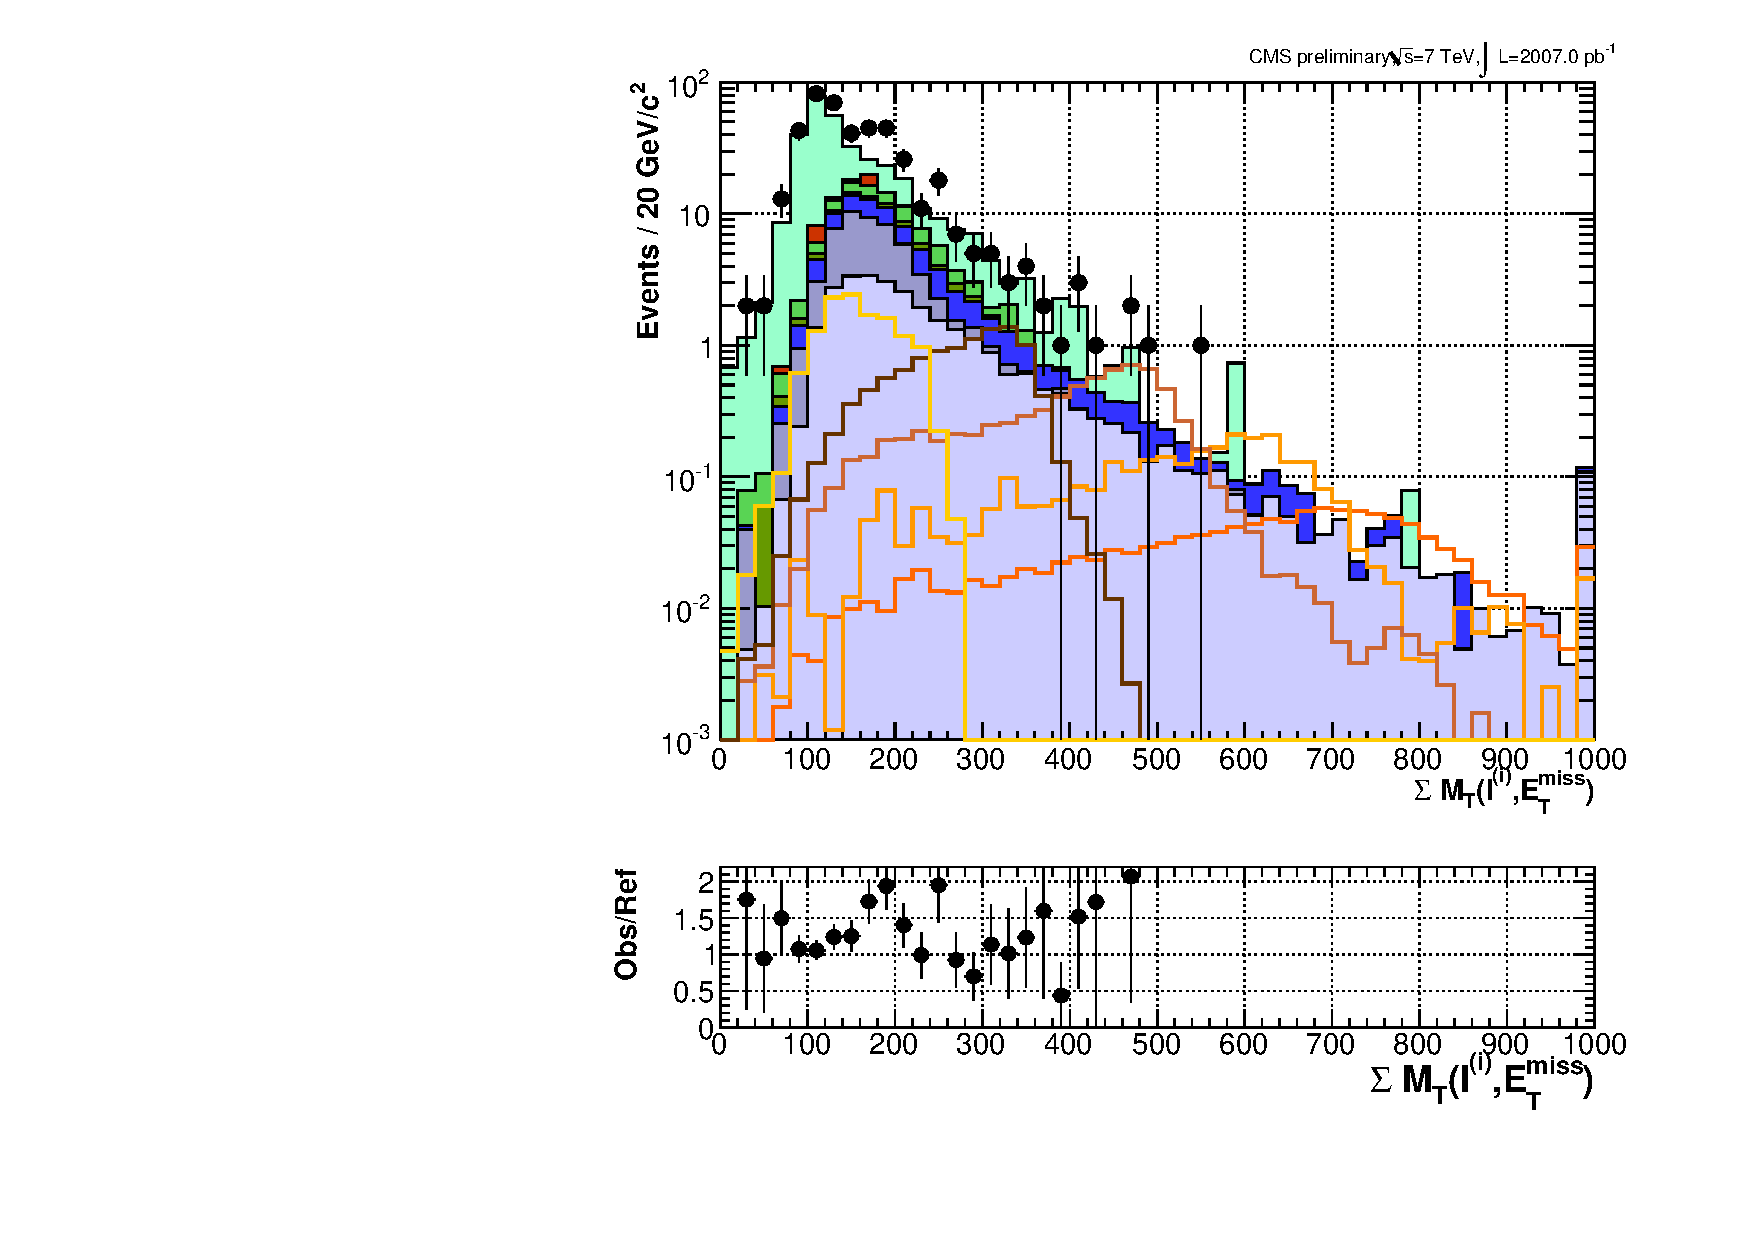
\includegraphics[width=0.3\textwidth]{img/cStack_mtSumLMet_ee_lveto_nob_redmetL}
\caption{Distribution of the input variables used to build the
  likelihood discriminant for data and MC in the di-muon ({\em top}) and di-electron ({\em bottom}) channels. 
  The plots show the events after the \RMET selection (loose working point).
}
\label{fig:input_redMET}
\end{center}
\end{figure}

It has been verified in the training that adding 
$\Delta \phi (lead-\ell, \ell\ell)$ (the longitudinal component of \RMET)
does not provide extra discrmination for the low (high) mass
selection, i.e. $m_{H^0}<(\geq$300~GeV/c$^2$.  
These variables are therefor not used for the low and high mass selections, correspondingly.

The distributions for the variables of interest are used as probability density functions (\PDF's)
to build a likelihood-based discriminant. 
For each event the value of the \PDF's 
evaluated for the reconstructed quantities of interest ($x_i$)
are multiplied in order to evaluate the probability that the event is signal-like or background-like. 
The following signal (or background) likelihood is therefore defined from the product of \PDF's:

\begin{equation}
\mathcal{L}_k = \displaystyle{\prod_{i=1}^N}~\mathcal{P}_{df}(x_i)
\label{eq:likelihood_component}
\end{equation}

Using Eq.~\ref{eq:likelihood_component} for signal ($\mathcal{L}_s$) and background ($\mathcal{L}_b$)
computed for each event we define our discriminator from the following ratio:

\begin{equation}
\mathcal{L}_R = \frac{\mathcal{L}_s}{\mathcal{L}_s+\mathcal{L}_b}
\label{eq:likelihood}
\end{equation}

The signal likelihod includes both the gluon-gluon fusion and VBF contributions to the ZZ and WW final states. 
The background likelihood is built from the simulated di-boson irreducible backgrounds.
The events used to train (i.e. define the pdf's) and evaluate the performance of the discriminator
are pre-selected in order to describe the pileup scenario expected in data. 
This procedure is used in order to have a training sample where all the events
of the same process enter with the same weight independently of the MC pileup re-weighting
described in Sec.~\ref{subsec:trigrec}.
The events pre-selected this way constitute approximately half of the total MC available for this analysis.
The ``unweighted'' sample is furthermore split in two independent samples
which are used correspondingly for training and testing of the discriminator.
The training is performed in different bins of jet multiplicity as this 
different signal signatures are expected and has it is expected to enhance the signal significance
especially in the low jet multiplicity bins.

The output of the discriminant for different jet multiplicity bins is shown in 
Fig~\ref{fig:likelihoodout_lowmass} for the low mass search and in 
Figs.~\ref{fig:likelihoodout_dimu} and ~\ref{fig:likelihoodout_diele} for the high mass search.
For the low (high) mass search the medium (tight) \RMET selection is applied before
evaluating the likelihood discriminator.
All distributions are shown for data and the full MC 
(including the partial signal and background sub-samples used for the training of the discriminator).
An overall fair agreement is observed between data and MC.
The performance of the discriminator is observed to be poorer for higher jet multiplicity bins 
where the residual top and $Z$ background tends to resemble the signal due to the pre-selection applied.

\begin{figure}[htp]
\begin{center}
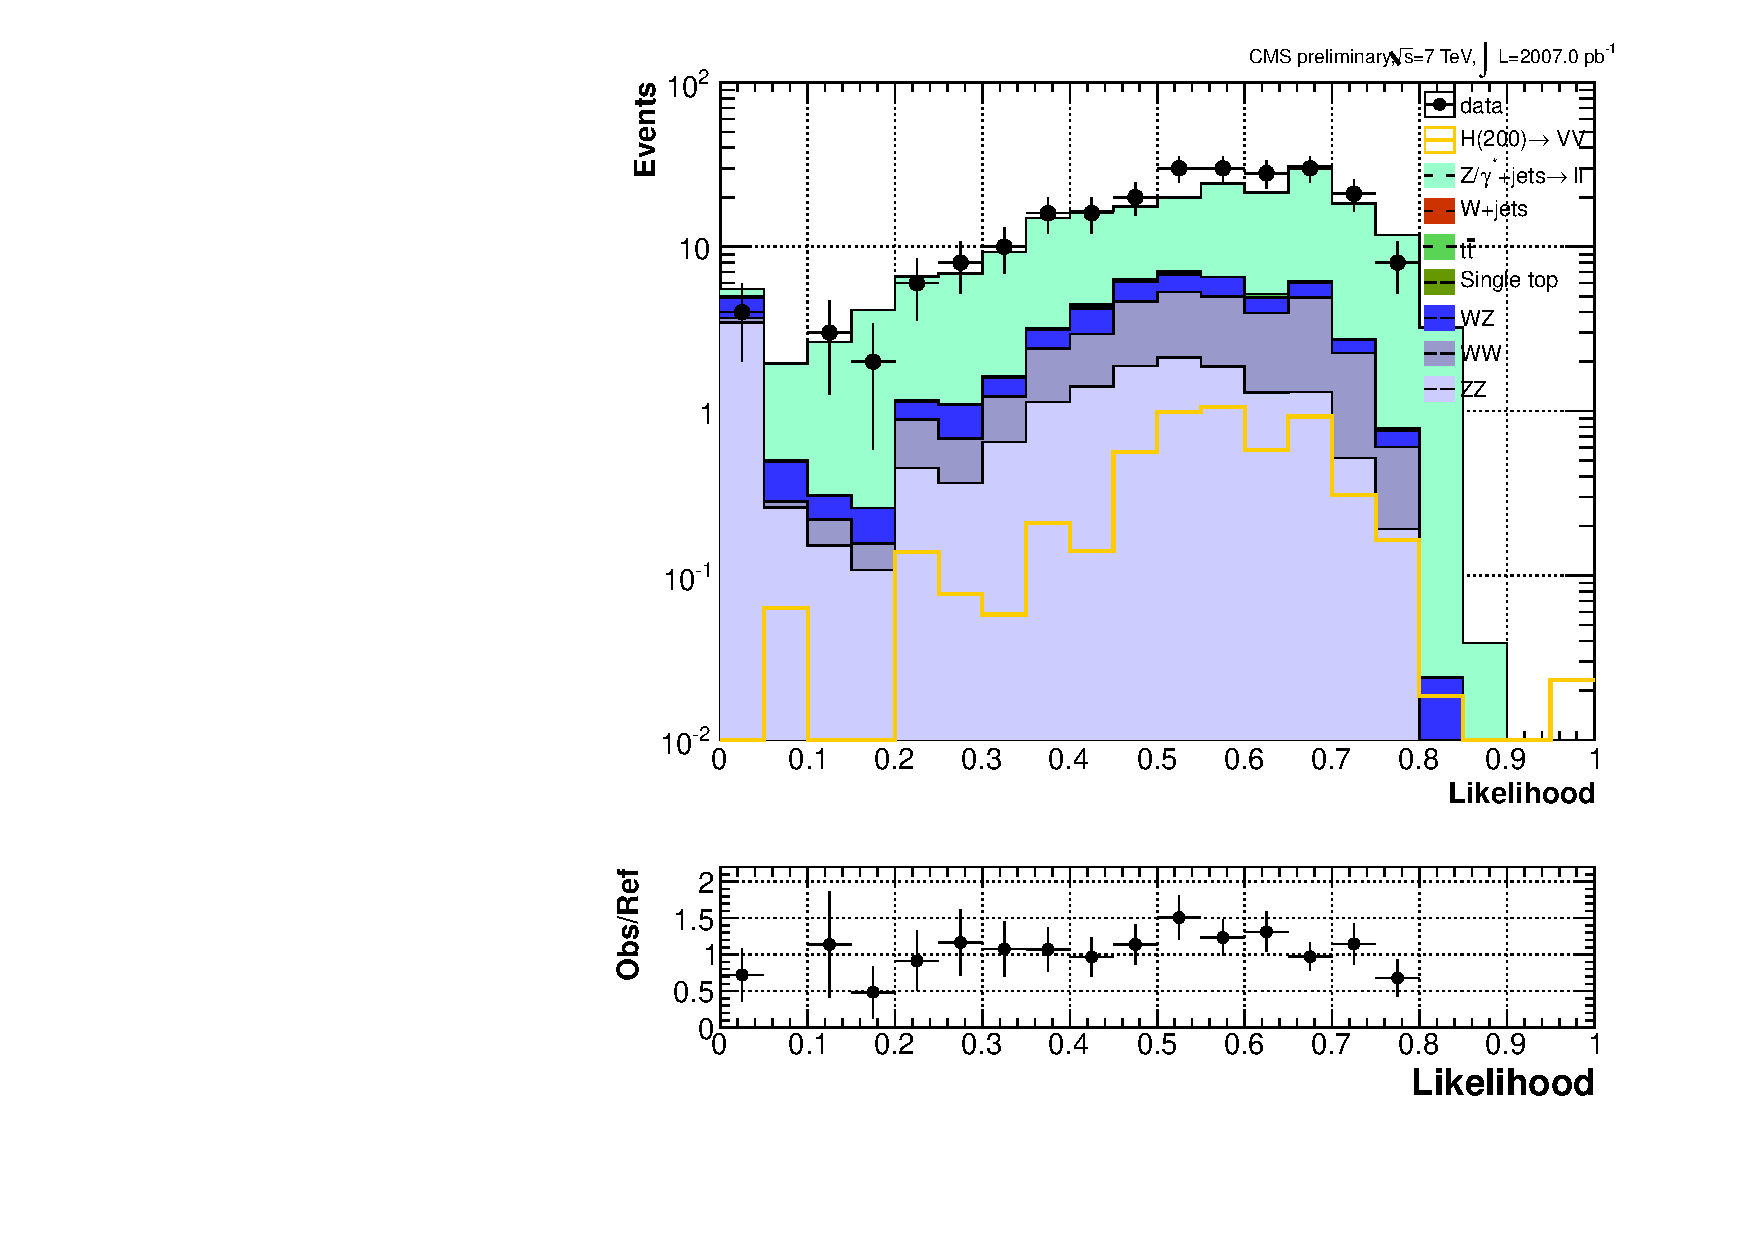
\includegraphics[width=0.3\textwidth]{img/mumueq0jets_Likelihood_200}
\includegraphics[width=0.3\textwidth]{img/mumueq1jets_Likelihood_200}
\includegraphics[width=0.3\textwidth]{img/mumugeq2jets_Likelihood_200}\\
\includegraphics[width=0.3\textwidth]{img/eeeq0jets_Likelihood_200}
\includegraphics[width=0.3\textwidth]{img/eeeq1jets_Likelihood_200}
\includegraphics[width=0.3\textwidth]{img/eegeq2jets_Likelihood_200}
\caption{Output of the $m_{H^0}=$200~GeV/c$^2$ likelihood discriminant for data and MC in the
  di-muon ({\em top}) and di-electron ({\em bottom}) final states. The different columns refer to different jet multiplicity bins:
  =0 jets ({\em left}), =1 jets ({\em center}) and $\geq$~2 jets ({\em right}).
}
\label{fig:likelihoodout_lowmass}
\end{center}
\end{figure}


\begin{figure}[htp]
\begin{center}
\includegraphics[width=0.3\textwidth]{img/mumueq0jets_Likelihoodtight_300}
\includegraphics[width=0.3\textwidth]{img/mumueq1jets_Likelihoodtight_300}
\includegraphics[width=0.3\textwidth]{img/mumugeq2jets_Likelihoodtight_300}\\
\includegraphics[width=0.3\textwidth]{img/mumueq0jets_Likelihoodtight_400}
\includegraphics[width=0.3\textwidth]{img/mumueq1jets_Likelihoodtight_400}
\includegraphics[width=0.3\textwidth]{img/mumugeq2jets_Likelihoodtight_400}\\
\includegraphics[width=0.3\textwidth]{img/mumueq0jets_Likelihoodtight_500}
\includegraphics[width=0.3\textwidth]{img/mumueq1jets_Likelihoodtight_500}
\includegraphics[width=0.3\textwidth]{img/mumugeq2jets_Likelihoodtight_500}\\
\includegraphics[width=0.3\textwidth]{img/mumueq0jets_Likelihoodtight_600}
\includegraphics[width=0.3\textwidth]{img/mumueq1jets_Likelihoodtight_600}
\includegraphics[width=0.3\textwidth]{img/mumugeq2jets_Likelihoodtight_600}
\caption{Output of the likelihood discriminant for data and MC in the
  di-muon final state. The different columns refer to different jet multiplicity bins:
  =0 jets ({\em left}), =1 jets ({\em center}) and $\geq$~2 jets ({\em right}).
  From {\em top} to {\em bottom} different signal masses are shown: from 300 to 600 GeV/c$^2$
  in steps of 100~GeV/c$^2$.
}
\label{fig:likelihoodout_dimu}
\end{center}
\end{figure}

\begin{figure}[htp]
\begin{center}
\includegraphics[width=0.3\textwidth]{img/eeeq0jets_Likelihoodtight_300}
\includegraphics[width=0.3\textwidth]{img/eeeq1jets_Likelihoodtight_300}
\includegraphics[width=0.3\textwidth]{img/eegeq2jets_Likelihoodtight_300}\\
\includegraphics[width=0.3\textwidth]{img/eeeq0jets_Likelihoodtight_400}
\includegraphics[width=0.3\textwidth]{img/eeeq1jets_Likelihoodtight_400}
\includegraphics[width=0.3\textwidth]{img/eegeq2jets_Likelihoodtight_400}\\
\includegraphics[width=0.3\textwidth]{img/eeeq0jets_Likelihoodtight_500}
\includegraphics[width=0.3\textwidth]{img/eeeq1jets_Likelihoodtight_500}
\includegraphics[width=0.3\textwidth]{img/eegeq2jets_Likelihoodtight_500}\\
\includegraphics[width=0.3\textwidth]{img/eeeq0jets_Likelihoodtight_600}
\includegraphics[width=0.3\textwidth]{img/eeeq1jets_Likelihoodtight_600}
\includegraphics[width=0.3\textwidth]{img/eegeq2jets_Likelihoodtight_600}
\caption{Output of the likelihood discriminant for data and MC in the
  di-electron final state. The legend is similar to Fig~\ref{fig:likelihoodout_dimu}.
}
\label{fig:likelihoodout_diele}
\end{center}
\end{figure}

\clearpage

%%
%% VBF selection
%%
\subsection{Vector Boson Fusion search}
\label{subsec:vbfsearch}

The search of the Higgs boson produced via vector boson fusion mainly relies on the VBF tagging selection described in Sec.~\ref{subsec:trigrec}.
After this tagging, the background is already reduced by a significant factor ($\sim 4\times10^{-4}$).
The backgrounds can be further reduced by applying the third lepton-veto and by requiring significant missing transverse energy using the \RMET variable.
The \RMET threshold has been choosen to have a selection efficiency of $10^{-3}$ on Drell-Yan events
(cf. Sec.~\ref{subsec:redmet}).
It is shown that these simple cuts are sufficient to have an expected background yields below 1, as shown on Table~\ref{tab:vbfcutandcountyields}.
As it can be seen from the same table, the dominant background for the VBF selection are the $gg \rightarrow VV \rightarrow \geq 1\ell \geq 1\nu$ events

\begin{table}[htp]
\caption{Event yields after VBF selection for the di-electron and di-muon channel in events.}
\label{tab:vbfcutandcountSN}
\begin{center}
\begin{tabular}{cccccc} \hline\hline
{\bf Higgs mass (GeV/c$^2$)}        & {\bf 200}         & {\bf 300}         & {\bf 400}         & {\bf 500}         & {\bf 600}     \\\hline\hline
                                    &                   &                   &                   &                   &               \\\hline
\multicolumn{6}{c}{\bf$ee$ channel}\\\hline
S/B expected                        & $0.41 \pm 0.29$   & $0.51 \pm 0.37$   & $0.31 \pm 0.22$     & $0.17 \pm 0.12$     & $0.09 \pm 0.06$  \\\hline
\multicolumn{6}{c}{\bf$\mu\mu$ channel}\\\hline
S/B expected                        & $1.84 \pm 1.37$   & $1.79\pm1.30$     & $0.99\pm 0.72$      & $0.50\pm 0.37$     &  $0.27\pm 0.20$     \\\hline
\end{tabular}
\end{center}
\end{table}


\begin{table}[htp]
\caption{Event yields after VBF selection for the di-electron and di-muon channel in events.}
\label{tab:vbfcutandcountyields}
\begin{center}
\begin{tabular}{lcc} \hline\hline
{\bf Process}          & {\bf$ee$ channel}  & {\bf$\mu\mu$ channel} \\\hline
H(200)$\rightarrow$ VV & 0.329 $\pm$ 0.014  & 0.441 $\pm$ 0.072 \\
H(300)$\rightarrow$ VV & 0.408 $\pm$ 0.021  & 0.429 $\pm$ 0.022 \\
H(400)$\rightarrow$ VV & 0.246 $\pm$ 0.009  & 0.238 $\pm$ 0.0087 \\
H(500)$\rightarrow$ VV & 0.133 $\pm$ 0.011  & 0.121 $\pm$ 0.012 \\
H(600)$\rightarrow$ VV & 0.070 $\pm$ 0.002  & 0.0651 $\pm$ 0.0022 \\\hline
ZZ                     & 0.0248 $\pm$ 0.010 & 0.0197 $\pm$ 0.0095 \\
WW                     & 0.0151 $\pm$ 0.015 & \\
WZ                     & 0.0363 $\pm$ 0.020 & 0.0618 $\pm$ 0.026 \\
Single top             & 0.0249 $\pm$ 0.024 & 0.0495 $\pm$ 0.044 \\
$t\bar{t}$             & 0.310 $\pm$ 0.222  & 0.0580 $\pm$ 0.058 \\
W+jets                 &                    &  \\
Z/$\gamma^{*}$+jets$\rightarrow$ ll &  0.388 $\pm$ 0.28  & 0.513 $\pm$ 0.038 \\ \hline
Total expected                      &  0.799 $\pm$ 0.572 & 0.702 $\pm$ 0.175 \\\hline
Data                                & 1                  &  \\\hline\hline
\end{tabular}
\end{center}
\end{table}



%%
%%
%%
\subsection{Efficiency of the selection}
\label{subsec:selefficiency}

\FIXME: the following text is a placeholder to be updated with the final values to be used

Trigger, lepton identification and isolation efficiencies are determined from data using the tag and probe technique
~\cite{CMS-AN-2009-111} and ~\cite{CMS-TWIKI-GEN-tandp}.
In this subsection we summarize the results and corresponding uncertainties to be used for the final analysis.
Further details on the intermediate steps used to obtain these results can be found in App.~\ref{sec:app:leptonefficiency}.
Trigger efficiency is measured in data for each one of the triggers used in the analysis (cf. Sec~\ref{subsec:trigrec}).
Trigger efficiency is measured with respect to the offline identification and isolation. The resulting value is used to re-scale the event yields.
Lepton identification and isolation are measured for both data and MC selected events and the ratio of the two measurements is use to re-scale the final event yields.
The uncertainty on the efficiencies is estimated by:

\begin{itemize}
\item varying the fit shape used to model the Z-peak and the background side band;
\item varying the pileup scenario used for the fits to MC selected events; 
Two extreme cases are considered: without pileup and using the flat pileup distribution before applying the re-weighting discussed in Sec.~\ref{subsec:trigrec}.
\item comparing in MC the expected degradation of isolation as a function of the pileup and the differences between $Z\rightarrow\ell$ decays in $Z$ events and in signal.
Details can be found in App.~\ref{sec:app:leptonisolation};
\end{itemize}


%%
%% Background determination
%%
\subsection{Background determination}
\label{subsec:backgrounddet}

\FIXME: the following sections are to be expanded in a newer version of the note.
They summarize two contributions to the background determination of the instrumental background
and of top background from data.

%%%
%%% Instrumental background
%%%
\subsubsection{Data-driven estimation of the instrumental background}
\label{subsubsec:instrumentalbackground}

We use isolated photon candidates to model the instrumental background.
We study the jet multiplicity and scaling properties of these events
in order to better reproduce the ones expected in $Z$ boson production.
The study is separated in two regimes where two different jet multiplicity scaling properties are expected
and which correspond to the gluon-gluon and VBF productions of the Higgs boson.
The approach followed is summarized below and has been recently proposed by~\cite{Englert:2011pq}.

Photon candidates are selected from dedicated photon triggered samples.
The samples are summarized in Table~\ref{tab:instrbckgdatasamples}.

\begin{table}[htp]
\begin{center}
\caption{\MC and data samples analyzed for the estimation of the instrumental background.
For data the total integrated luminosity and the run range analyzed are shown.
For \MC the the cross section and the corresponding integrated luminosity of the analyzed sample are shown.
Z2 is used as a shortname for TuneZ2\_7TeV\_pythia6 and S* for Summer11-PU\_S*\_START42\_V11.
}          
\label{tab:instrbckgdatasamples}
\begin{tabular}{lcl} \hline\hline
\multicolumn{3}{c}{\bf Data} \\
Dataset                               & $L$~(pb$^{-1}$)               & Run range                          \\\hline
/Photon/Run2011A-May10ReReco-v1/AOD   &                               & {\small 160404-163869}             \\
/Photon/Run2011A-PromptReco-v4/AOD    &                               & {\small $>$163869}                 \\
{\bf Total}                           & {\bf }                        &                                    \\\hline
                                      &                               &                                    \\\hline
\multicolumn{3}{c}{\bf \MC} \\
Dataset                               & $\sigma$~(pb)                 & $L$~(pb$^{-1}$)                   \\\hline
/G\_Pt-15to30\_Z2/S3-v2/AODSIM        & 1.72$\times$10$^5$            &                                   \\
/G\_Pt-30to50\_Z2/S3-v2/AODSIM        & 1.67$\times$10$^4$            &                                   \\
/G\_Pt-50to80\_Z2/S3-v2/AODSIM        & 2.72$\times$10$^3$            &                                   \\
/G\_Pt-80to120\_Z2/S4-v2/AODSIM       & 4.47$\times$10$^2$            &                                   \\
/G\_Pt-120to170\_Z2/S3-v2/AODSIM      & 84.2                          &                                   \\
/G\_Pt-170to300\_Z2/S4-v2/AODSIM      & 22.6                          &                                   \\
/G\_Pt-300to470\_Z2/S3-v2/AODSIM      & 1.49                          &                                   \\
/G\_Pt-470to800\_Z2/S3-v2/AODSIM      & 0.132                         &                                   \\
/G\_Pt-800to1400\_Z2/S3-v2/AODSIM     & 3.48$\times$10$^{-3}$         &                                   \\
/G\_Pt-1400to1800\_Z2/S3-v2/AODSIM    & 1.26$\times$10$^{-5}$         &                                   \\\hline\hline
\end{tabular}
\end{center}
\end{table}

For each triggered event the highest $p_T$ photon trigger candidate is chosen.
The offline reconstructed photon is required to have a $E_T$ 
greater than that of the trigger threshold it fired.
Further identification and isolation requirements are made as summarized in Table~\ref{tab:photonsel}
and are based on~\cite{Khachatryan:2010fm}.

\begin{table}[htp]
\begin{center}
\caption{Photon selection requirements according to the region of reconstruction in the electromagnetic calorimeter.}
\label{tab:photonsel}
\begin{tabular}{lcc} \hline\hline
Variable                              & ECAL barrel                        & ECAL endcap                   \\\hline
$E_T$                                 & \multicolumn{2}{c}{trigger dependent}                              \\
$|\eta|$                              & $<$1.4442                          & 1.566$<|\eta|<$2.5            \\ 
$\sigma_{i\eta i\eta}$                & 0$<\sigma<$0.013                   & 0$<\sigma<$0.03               \\ 
$\sigma_{i\phi i\phi}$                & $>$0                               & -                             \\ 
seed rec. hit flag                    & $\neq$ kOutOfTime                  & -                             \\ 
$h/e$                                 & $<$0.05                            & $<$0.5                        \\ 
Tracker isolation                     & \multicolumn{2}{c}{$<$2.0 + 0.001$E_T$}                            \\ 
ECAL isolation                        & \multicolumn{2}{c}{$<$4.2 + 0.003$E_T$}                            \\ 
HCAL isolation                        & \multicolumn{2}{c}{$<$2.2 + 0.001$E_T$}                            \\\hline 
\end{tabular}
\end{center}
\end{table}


%%%
%%% Top 
%%%
\subsubsection{Data-driven estimation of residual top background}
\label{subsubsec:topbackground}

%%
%%
%%
\clearpage
\subsection{Systematic uncertainties}
\label{subsec:systunc}

In the analysis just described different sources of systematic uncertainties might affect the number of observed events and/or the shapes of the discriminators.
The main sources of systematic uncertainties are summarized and estimated in the following paragraphs.

{\bf Instrumental uncertainties}

%%%%
{\it Luminosity}:

The uncertainty on the integrated luminosity is estimated to be 4.5\%. This affects the predicted event yields for our signal
and also the predicted event yields for all backgrounds which are not estimated directly from data.
It's a fully correlated systematic among all processes fully predicted from MC.

%%%%
{\it Jet energy scale and resolution}:

The uncertainty in the calibration of the jet energy scale affects directly the categorization of the events in different jet
multiplicity bins and as potential VBF candidates. Notice that this effect contributes to a cross-bin migration but 
it also contributes an overall increase/decrease of the number of selected events as due to miscalibration of the energy flow
the \MET measurement (and consequently the \RMET variable) are affected.
The estimate of the jet energy scale uncertainty is performed varying independently the jet energy scale up and down by 1-$\sigma$
as measured by the Jet/MET group~\cite{CMS-TWIKI-GEN-jec}. The variation corresponds to a simple re-scaling of the jet 4-momentum as:
$P \rightarrow P\cdot (1\pm \sigma_{JES}/p_T)$ where $\sigma_{JES}$ is the absolute uncertainty on the jet energy scale
which is parametrized as function of the $p_T$ and $\eta$ of the jet
\footnote{The parametrizations are taken from the database corresponding to the global tag used to process data.
Details can be found at~\cite{CMS-TWIKI-GEN-jec}.}.
This variation affects the energy imbalance of the detector and it is therefore propagated to re-compute the \MET measurement as:

\begin{equation}
\vec{E}_{T}^{miss'} = \vec{E}_{T}^{miss} - \displaystyle{\sum_{jets}} ( \pm \frac{\sigma_{JES}}{p_T}) \cdot \vec{p}_{T} 
\label{eq:jesmet}
\end{equation}

where the $\pm$ choice correponds to an up/down variation of the jet energy scale uncertainty.
The uncertainties are considered separately, also for the purpose of the statistical analysis in Sec.~\ref{sec:excllimits}
as the different variations lead to different jet bin migrations.

Likewise the resolution of the jet reconstruction, i.e. the distribution of the detector response
to an imcoming jet clustered from stable particles after parton showering, affects the analysis
in a similar way as the one described for the jet energy scale uncertainty.
The evaluation of this effect is important has punch-through energetic particles
or the presence of dead channels in the detector introduce asymmetric effects in the detector response.
The evaluation of this effect is simplified by the fact that we do not use the generator level jets
but the reconstructed ones and smear their four momenta according to the resolutions expected from simulation~\cite{CMS-AN-2010-121}.
For each event, the $p_T$,$\eta$ and $\phi$ of the reconstructed jets are smeared and the effect is propagated to the
\MET measurement using Eq.~\ref{eq:jesmet}.
In the case of the jet energy resolution effect we take the absolute value observed as the estimate for the
the two sided (positive/negative) uncertainty.

Tab.~\ref{tab:jesuncs} and Tab..~\ref{tab:jeruncs} summarizes the estimates of the uncertainties due to jet energy scale and resolution
for a specific mass selection. Similar systematic uncertainties are computed independently depending on the event selection applied
but are note reproduced for simplicity of the manuscript
\footnote{The actual values used can be found in the datacards used for the statistical analysis of Sec.~\ref{sec:excllimits}
which are available in CVS~\cite{cvscode}.}.
The variation of jet energy resolution and the two independent variations of the jet energy scale
are a fully correlated systematic among all processes.


\begin{table}[htp]
\begin{center}
\caption{Relative dystematic uncertainty due to the variation of the jet energy scale for a mass selection of 300~GeV/c$^2$.
The up (down) variations are quoted separately as super(sub)-script for each event category and process.}
\label{tab:jesuncs}
\begin{tabular}{lcccccc} \hline\hline
\multirow{2}{*}{Event category}     & \multicolumn{3}{c}{$\mu\mu$}                                 & \multicolumn{3}{c}{$ee$} \\
                                    & =0 jets            & =1 jets            & $\geq$ 2 jets      & =0 jets            & =1 jets       & $\geq$ 2 jets \\\hline
Signal                              & $^{0.995}_{1.073}$ & $^{0.991}_{1.032}$ & $^{0.989}_{0.930}$ & $^{0.967}_{1.072}$ & $^{0.989}_{1.021}$ & $^{0.986}_{0.931}$  \\\hline
W+jets                              & $^{1.000}_{1.000}$ & $^{1.000}_{1.000}$ & $^{1.000}_{1.000}$ & $^{1.000}_{1.000}$ & $^{1.000}_{1.000}$ & $^{1.000}_{1.000}$  \\
Z/$\gamma^{*}$+jets$\rightarrow$ ll & $^{1.000}_{1.000}$ & $^{1.000}_{1.071}$ & $^{0.771}_{1.102}$ & $^{1.000}_{1.000}$ & $^{1.000}_{1.000}$ & $^{0.986}_{1.039}$  \\
\ttbar                              & $^{1.000}_{1.000}$ & $^{1.000}_{0.845}$ & $^{1.098}_{0.929}$ & $^{1.000}_{1.000}$ & $^{1.000}_{1.024}$ & $^{1.000}_{0.994}$  \\
Single Top                          & $^{1.000}_{1.000}$ & $^{1.000}_{1.204}$ & $^{1.340}_{1.000}$ & $^{1.000}_{1.000}$ & $^{1.060}_{1.120}$ & $^{1.000}_{0.769}$  \\
WW                                  & $^{1.012}_{1.000}$ & $^{1.205}_{1.091}$ & $^{1.000}_{0.973}$ & $^{1.016}_{1.000}$ & $^{1.102}_{1.095}$ & $^{1.118}_{0.889}$  \\
WZ                                  & $^{0.990}_{1.058}$ & $^{1.002}_{1.031}$ & $^{0.969}_{0.917}$ & $^{0.999}_{1.078}$ & $^{0.964}_{1.019}$ & $^{1.009}_{0.939}$  \\
ZZ                                  & $^{0.999}_{1.050}$ & $^{0.991}_{0.966}$ & $^{1.023}_{0.892}$ & $^{1.002}_{1.061}$ & $^{0.999}_{0.970}$ & $^{0.994}_{0.917}$  \\\hline\hline
\end{tabular}
\end{center}
\end{table}


\begin{table}[htp]
\begin{center}
\caption{Relative systematic uncertainty due to the variation of the jet energy resolution for a mass selection of 300~GeV/c$^2$.}
\label{tab:jeruncs}
\begin{tabular}{lcccccc} \hline\hline
\multirow{2}{*}{Event category}     & \multicolumn{3}{c}{$ee$}          & \multicolumn{3}{c}{$\mu\mu$} \\
                                    & =0 jets & =1 jets & $\geq$ 2 jets & =0 jets & =1 jets & $\geq$ 2 jets \\\hline
Signal                              & 1.115   & 1.118   & 0.963         & 1.116   & 1.089   & 0.9760 \\\hline
W+jets                              & 1.000   & 1.000   & 1.000         & 1.000   & 1.000   & 1.000 \\
Z/$\gamma^{*}$+jets$\rightarrow$ ll & 1.000   & 2.000   & 1.481         & 1.000   & 2.000   & 2.000  \\
\ttbar                              & 1.000   & 0.757   & 1.202         & 1.000   & 1.024   & 1.055  \\
Single Top                          & 1.317   & 0.922   & 1.221         & 1.031   & 1.006   & 0.868 \\
WW                                  & 1.011   & 1.430   & 1.416         & 0.991   & 1.121   & 1.122 \\
WZ                                  & 1.090   & 1.066   & 1.024         & 1.084   & 1.037   & 0.963  \\
ZZ                                  & 1.055   & 0.989   & 0.869         & 1.068   & 0.986   & 0.914 \\\hline\hline
\end{tabular}
\end{center}
\end{table}




%%%%
{\it $b$-tagging}:

The effective $b$-tagging uncertainty is measured from data using a $b$-enriched sample~\cite{CMS-PAS-BTV-11-001}.
The data-driven measurement yields data/MC scale correction factors
for the $b$-tagging and mistag rates. These scale factors are approximately constant and independent of the kinematics of the jet.
The scale factors can be applied to correct the MC expected event yields and the
corresponding uncertainties can be used to project the systematic uncertainty of the analysis due to the use of $b$-tagging.
The procedure adopted is the following: let $N_b$ ($N_q$) be the number of $b$ ($udscg$) jets observed in a pre-tagged event
\footnote{The flavor of the jet is determined assessing MC truth.}.
We assign the probability that the event will not generate any tag based
on the knowledge of $\varepsilon_b$ ($\varepsilon_q$), i.e the average b-tagging (mistagging) efficiency in the simulation,
the data-derived scale factor $S_F^b$ ($S_F^q$) for the $b$-tagging (mistagging) effiency
and the number of $b$ ($udscg$) jets as follows:

\begin{equation}
p_0 = (1-S_F^b\varepsilon_b)^{N_b}(1-S_F^q\varepsilon_q)^{N_q}
\label{eq:prob0btags}
\end{equation}

In order to propagate the uncertainty of the scale factors to the probability of an event to pass 
the $b$-tag veto, one applies the standard the error propagation:

\begin{equation}
\delta p_0 = \sqrt{ 
[N_b \sigma_{S_F^b} \varepsilon_b (1-S_F^b\varepsilon_b)^{N_b-1}(1-S_F^q\varepsilon_q)^{N_q} ]^2 +
[N_q\sigma_{S_F^q} \varepsilon_q (1-S_F^b\varepsilon_b)^{N_b}(1-S_F^q\varepsilon_q)^{N_q-1} ]^2 }
\label{eq:prob0btagsunc}
\end{equation}

The predicted number of events with 0 b-tags, i.e., passing the $b$-tagging veto described in Sec.~\ref{subsec:trigrec},
is therefore obtained from the sum of the weights derived for each event in the pre-tagged sample, i.e.:

\begin{equation}
N_0 = \displaystyle{\sum_{k=1}^{N_{events}}} p_i^{0}
\label{eq:passbveto}
\end{equation} 

and the corresponding uncertainty associated to the prediction of Eq.~\ref{eq:passbveto} is given by

\begin{equation}
\delta N_0 = \displaystyle{\sum_{k=1}^{N_{events}}} \delta p_i^{0}
\label{eq:passbvetounc}
\end{equation} 

We use therefore the result of ~\ref{eq:passbvetounc} as the estimate of the $b$-veto uncertainty due to the uncertainty
on the $b$ and mistag rates. The uncertainty is evaluated in the pre-tagged sample (after the 3$^{rd}$ lepton veto) and it is assumed
for the rest of the selection. 


%%%%
{\it Pileup}:

Pileup can induce a systematic uncertainty which affects mainly the \MET measurement but also the isolation and energy scale of the objects.
For the moment we take the most conservative estimate of the pileup uncertainty by comparing the event yields without weighting the MC.  
This yields a uniform pileup scenario up to 10 in-time interactions in simulation and has the benefit of testing qualitatively the robustness of the analysis.
Tab.~\ref{tab:puuncs} summarizes the estimate of the pileup uncertainty for a given mass point selection.
For most processes one can observe an increase of events with higher multiplicity of jets, 
as previous discussed in Sec.~\ref{subsec:trigrec}.
The exception seems to be single top for which the $b$-jet seems to be missed more often in high pileup scenario.
A loss of efficiency in some bins might also be related to a loss of efficiency in the isolation selection of the leptons.
Similar uncertainties are obtained for the other mass points but omitted for simplicity of the manuscript.
This is considered to be a fully correlated systematic among all processes.

\begin{table}[htp]
\begin{center}
\caption{Systematic uncertainty due to the variation of pileup for a mass selection of 300~GeV/c$^2$.}
\label{tab:puuncs}
\begin{tabular}{lcccccc} \hline\hline
\multirow{2}{*}{Event category}     & \multicolumn{3}{c}{$\mu\mu$}          & \multicolumn{3}{c}{$ee$} \\
                                    & =0 jets & =1 jets & $\geq$ 2 jets & =0 jets & =1 jets & $\geq$ 2 jets \\\hline
Signal                              & 0.966   & 1.016   & 1.043         & 0.989   & 1.006   & 1.049         \\\hline
W+jets                              & 1.000   & 1.000   & 1.000         & 1.000   & 1.000   & 1.000        \\
Z/$\gamma^{*}$+jets$\rightarrow$ ll & 1.000   & 1.390   & 1.090         & 1.000   & 1.373   & 1.506        \\
\ttbar                              & 1.000   & 0.797   & 1.173         & 1.000   & 0.924   & 0.983        \\
Single Top                          & 1.267   & 1.031   & 0.906         & 0.925   & 1.078   & 0.965        \\
WW                                  & 1.026   & 0.799   & 1.169         & 1.050   & 1.062   & 1.106         \\
WZ                                  & 1.085   & 0.989   & 1.015         & 1.083   & 0.983   & 1.068        \\
ZZ                                  & 1.028   & 1.028   & 1.135         & 1.038   & 0.983   & 1.019        \\\hline\hline
\end{tabular}
\end{center}
\end{table}

   
%%%%
{\bf Theoretical uncertainties}

%%%%
{\it Cross sections}:

For all background process which are not estimated from data the uncertainty on the cross section has to be taken into account.
We use the values quoted in~\cite{CMS-TWIKI-GEN-xsec} and in ~\cite{CMS-TWIKI-GEN-xsecst}.
The cross section for the signal is also affected by the theoretical uncertainty.
The theory error breakdown for the cross sections usually takes into account the 
scale uncertainties (factorization and renormalization are individually varied by a factor 2 up and down)
and PDF uncertainties (from the uncorrelated combination of the independent fluctuations of the NLO PDF parameters).
The uncertainty for the signal cross section is considered from the combination of the normalization/factorization scale uncertainties and PDF+$\alpha_S$
as reported in~\cite{LHCHiggsCrossSectionWorkingGroup:2011ti}.
Table~\ref{tab:xsecuncs} summarizes the final uncertainties considered for the production cross sections of the different processes

\begin{table}[htp]
\begin{center}
\caption{Theoretical uncertainties on the production cross-sections of the different signal and background processes.
The contributions included for each uncertainty are described in the text.
The breakup of the uncertainties for each sub-channel is shown explicitly for signal (gluon-gluon/VBF) and for single top (t-,s-,tW-channel).}          
\label{tab:xsecuncs}
\begin{tabular}{lcl} \hline\hline
Process                                           & Relative uncertainty (\%) \\\hline
H(200)                                            & 7.7 {\small (7.4 / 2.2)}\\
H(300)                                            & 7.7 {\small (7.1 / 2.8)}\\
H(400)                                            & 8.0 {\small (7.2 / 2.8)}\\
H(500)                                            & 8.6 {\small (7.6 / 2.8)}\\
H(600)                                            & 9.3 {\small (8.1 / 2.8)}\\\hline
Single Top                                        & 3.3 {\small (3.9 / 4.4 / 7.6)} \\
W                                                 & 4.9 \\
$Z/\gamma^{*}\rightarrow \ell$ (M$>$50 GeV/c$^2$) & 4.3 \\
\ttbar                                            & 6.1 \\
WW                                                & 3.5 \\
WZ                                                & 3.8 \\
ZZ                                                & 2.5 \\\hline\hline
\end{tabular}
\end{center}
\end{table}

The uncertainty on the cross section is assigned independently for each process predicted from MC.

%%%%%
{\it Single top tW contribution}

The tW process is usually defined from the minimum interference with the \ttbar production
by removing diagrams in which an internal top quark line in \ttbar production is converted into a final state $b$ quark
by emission of a $W$ boson. This approach is used by default and should be compared
with the result of diagram subtraction which includes terms to cancel locally the \ttbar contribution
which maintain gauge invariance. Details can be found in~\cite{s:Giamm2010}.
An extra systematic uncertainty is assigned to the tW process due to the differences found
between the standard diagram removal (DR) and diagram subtraction (DS) scheme. 
The differences found after the applying the medium selection cut for the \RMET variable are summarized in Tab~\ref{tab:twuncs}.
We assume this systematic uncertainty for all the subsequent mass point selections.

\begin{table}[htp]
\begin{center}
\caption{Systematic uncertainty affecting the final selection due to the theoretical definition of the $tW$ cross section.}
\label{tab:twuncs}
\begin{tabular}{lcccc} \hline\hline
Event category                                    & =0 jets & =1 jets & $\geq$ 2 jets & VBF \\\hline
Systematic uncertainty                            &         &         &               & \\\hline\hline
\end{tabular}
\end{center}
\end{table}
 


%%%%%
{\it Higgs $p_T$ spectrum}

The generator used to describe the gluon-gluon production of the Higgs boson (\Powheg) is a NLO generator.
The spectrum and cross section predicted by the event generator can therefore be corrected to a most NNLO+NNLL calculation
using the HqT program. The reweighing procedure of the Higgs $p_T$ spectrum is affected by 
similar uncertainties as the ones described for the theoretical cross section and can therefore be evaluated in similar way as described in the previous paragraphs.
To propagate these effects in our analysis we replace the nominal reweighing of the Higgs $p_T$ in the simulation
by weights corresponding to the up/down variations of the factorization and renormalization scales~\cite{CMS-TWIKI-GEN-higgspt}. 
The variation of the final event yields in signal is therefore assigned as a systematic uncertainty.
The uncertainty on Higgs $p_T$ spectrum affects only the signal predictions
and it is summarized in Tab.~\ref{tab:hptuncs} for a given mass point as an example.
For each source (renormalization or factorization scale) the uncertainty is taken conservatively as the maximum
variation observed (after varying the nominal scale by a factor of 2 up and down).
Similar results are obtained for other mass points but omitted for simplicity of the manuscript.
As there are cross-contaminations between the different jet and VBF bins this uncertainty
has to be considered for all the event categories.

\begin{table}[htp]
\begin{center}
\caption{Systematic uncertainties affecting the final selection due to the event generator used to model the 300~GeV/c$^2$ signal.
Two sources of systematic uncertainty affecting the prediction for the Higgs boson $p_T$ are quoted.}
\label{tab:hptuncs}
\begin{tabular}{lcccccc} \hline\hline
\multirow{2}{*}{Event category}     & \multicolumn{3}{c}{$\mu\mu$}          & \multicolumn{3}{c}{$ee$} \\
                                    & =0 jets & =1 jets & $\geq$ 2 jets & =0 jets & =1 jets & $\geq$ 2 jets  \\\hline
Renormalization                     & 0.999   & 1.003   & 1.001         & 1.003   & 1.002   & 1.000   \\
Factorization                       & 0.968   & 0.994   & 0.997         & 0.974   & 0.992   & 0.997 \\\hline\hline 
\end{tabular}
\end{center}
\end{table}


%
%
%
\clearpage
\section{Exclusion limits}
\label{sec:excllimits}

\FIXME: This section will be filled in the next version of the note. 
Include statistical analysis based on the results obtained in the previous section.
Combine ee+$\mu\mu$ channel in the 3-jet multiplcity bins and compare the cut and count
analysis performance with the multivariate analysis performance.
Add combination with VBF for the cut and count analysis.
Include stand-alone contribution from the VBF analysis like shown in Tab.~\ref{tab:vbflimits}.

\begin{table}[htp]
\begin{center}
\caption{Limits on the predicted SM qq$\rightarrow$H cross section set from the selected data.
The 68\% uncertainty on the expected limit is included for reference.
The uncertainty includes luminosity and MC statistics.}
\label{tab:vbflimits}
\begin{tabular}{lccccc} \hline\hline
\multirow{2}{*}{$\sigma/\sigma_{SM}$} & \multicolumn{5}{c}{$m_{H^0}$ (GeV/c$^2$)} \\
                                      & 200  & 300    & 400  & 500  & 500 \\\hline
Expected (MC)                         & 5.7 $\pm$ 1.8 & 5.2 $\pm$ 1.6 & 9.0 $\pm$ 3.0 & 17.2 $\pm$ 5.2 & 32 $\pm$ 10  \\
Data                                  & 5.1           & 4.7           & 8.24        & 15.7          & 29.6 \\\hline\hline
                                      &      &      &      &      & \\
{\small Obs=0  (hyp.)}                & {\small 3.95} & {\small 3.63} & {\small 6.29} & {\small 11.9} & {\small 22.5} \\
\end{tabular}
\end{center}
\end{table}


%
% CONCLUSIONS
%
\clearpage
\section{Conclusions}
\label{sec:conclusions}

\FIXME: this document is still work in progress. 
The conclusions will be added in the second version of the document.

%% **DO NOT REMOVE BIBLIOGRAPHY**
\bibliography{auto_generated}   % will be created by the tdr script.

\clearpage

%
% APPENDIX
%
\appendix
\section{Lepton isolation}
\label{sec:app:leptonisolation}

In this section we focus on two specific aspects affecting the determination of lepton isolation efficiency:
the contamination from pileup and the differences between leptons in the $Z\rightarrow ll$ sample and in the Higgs sample.

The presence of pileup is expected to contribute to the degradation of the isolation, especially 
through the neutral particles which cannot be associated to the vertex.
The deviation introduced in the isolation by the average energy density deposition in the detector from pileup
can be estimated using the $\rho$-parameter computed using the fast jet algorithm~\cite{Cacciari:2007fd}.
As the average values for $\rho$, $I_{photons}$ and $I_{neutral~hadrons}$ are expected to increase differently as a function of the number of pileup events
a linear parameterization can be derived for each case and used to correct the isolation in average.
The results of these parameterizations are shown for in Fig~\ref{fig:isolprofile} for a simulated sample of $Z\rightarrow \mu\mu$.
The width of the distributions of the previous variables is also affected by the pileup and in the case of the $\rho$ a non-linear behavior is observed.
In this study we choose therefore not to perform any correction for the isolation based on the pileup contamination as estimated from 
the $\rho$ parameter due to the fact that events with large fluctuations of $\rho$ can lead to overcorrections of the lepton isolation leading to an increase
of the contamination from non-isolated lepton candidates.
The slope of the isolation profile is used to assign a systematic uncertainty on the isolation efficiency of 0.8\%
for both electrons and muons.

\begin{figure}[htp]
\begin{center}
\includegraphics[width=0.9\textwidth]{img/muonIsolationProfile}
\caption{
Isolation and $\rho$ profiles in simulated $H\rightarrow VV\rightarrow 2\mu 2\nu_{\mu}$ events.
The average (RMS) of the distributions is shown as function of the number of generated pileup events on the {\em left} ({\em right}).}
\label{fig:isolprofile}
\end{center}
\end{figure}

The efficiency of the isolation requirement is determined from data using the tag-and-probe method.
This method relies on the kinematics of $Z\rightarrow ll$ events which may differ slightly from the kinematics
of the signal, i.e. $H\rightarrow VV\rightarrow 2l2\nu$. The difference is not expected to be observed in the absolute isolation of the leptons
as the jet activity is not substantially different and as the pileup conditions are similar.
However, as the $p_T$ distribution of the leptons is different, being the leptons from $Z$ events usually softer, 
a difference arises in the relative isolation, as the ratio of the absolute isolation to the $p_T$ of each lepton is considered.
This effect is illustrated in Fig.~\ref{fig:zvshlepkinematics} where the $p_T$, absolute isolation and relative isolation
of the leptons matched to the decays of the Z bosons are compared. 
From this study we conclude that the efficiency of the relative isolation in $\mu\mu$ ($ee$) events is 0.8\% (0.5\%) smaller in Higgs events with respect to $Z$ events. 
Therefore we assign this number as a systematic uncertainty on the efficiency computed from data using the tag-and-probe method. 

\begin{figure}[htp]
\begin{center}
\includegraphics[width=0.3\textwidth]{img/matchedmuon_pt}
\includegraphics[width=0.3\textwidth]{img/matchedmuon_absiso}
\includegraphics[width=0.3\textwidth]{img/matchedmuon_reliso}\\
\includegraphics[width=0.3\textwidth]{img/matchedelectron_pt}
\includegraphics[width=0.3\textwidth]{img/matchedelectron_absiso}
\includegraphics[width=0.3\textwidth]{img/matchedelectron_reliso}
\caption{Transverse momentum ({\em left}), absolute isolation ({\em center}) and relative isolation ({\em right}) of the
reconstructed muons ({\em top}) and electrons ({\em bottom}) matched to the generator level
leptons fro the $Z$ boson decay in simulation.
The standard $Z$ production is compared to the production in the Higgs decay chain considering an hypothetical mass of 200~GeV/c$^2$.}
\label{fig:zvshlepkinematics}
\end{center}
\end{figure}



\section{Cut based optimization}
\label{sec:app:cutbasedoptimization}

In this section we summarize the procedure adopted to optimized the selection of the cut based analysis for the search for Higgs boson.
A simple approach has been taken by considering three variables which show discriminating power for the Higgs signal.
These variables are:

\begin{description}
\item[$\delta\phi^{ll}$] - the azimuthal angle between the two leptons that constitute the dilepton candidate. The angle is expected to be significantly smaller for final state leptons from Higgs with large mass;
\item[\RMET (longitudinal)] - the longitudinal component of \RMET. This specific projection is expected to show the sensitivity to events in which the two Z bosons from the Higgs decay are recoiling against each other.
For low mass Higgs, the production of extra jets, might however lead to a boost of the overall system in which both Z's can be produced along the same hemisphere. 
In these boosted topologies the longitudinal component of \RMET is expected to point along the dilepton direction;
\item[$\sum M_{T}(l^i,E_{T}^{miss})$] - the sum of the transverse mass of each lepton with the \MET vector. This variable is chosen as no full mass reconstruction is possible in the final state under study.
The full transverse mass of the system could be used but by requiring both the dilepton and the \MET source to be the same, i.e., a $Z$ boson, introduces an artificial kinematic limit on all backgrounds.;
\end{description}

The  variables used to define a loose selection region where the presence of signal is more significative, i.e. where $f=S/\sqrt{S+B}$ is maximized.
As tighter selections also lead to a depletion of signal, the cuts are selected in the rising edge of the $f$ variable.
Fig.~\ref{fig:varcutopt} summarizes the distributions obtained for the $f$ variable after requiring that the instrumental
background is reduced by 10$^{-3}$ (medium working point for \RMET selection, as defined in Sec.~\ref{subsec:redmet}.
Although differences are found between different jet multiplicity bins, they are not considered to tune further the cuts,
as the $f$-curves show similar rising edges. Therefore, inclusive selection cuts are chosen.

\begin{figure}[htp]
\begin{center}
\includegraphics[width=0.64\textwidth]{img/FoM_200}\\
\includegraphics[width=0.64\textwidth]{img/FoM_300}\\
\includegraphics[width=0.64\textwidth]{img/FoM_400}\\
\includegraphics[width=0.64\textwidth]{img/FoM_500}\\
\includegraphics[width=0.64\textwidth]{img/FoM_600}
\caption{Figure of merit for different Higgs masses for different variables and for events with different jet multiplicities. 
The cut chosen for each variable is overlaid in the figures.
All backgrounds, as predicted by simulation, are considered.}
\label{fig:varcutopt}
\end{center}
\end{figure}

\section{Lepton Efficiency}
\label{sec:app:leptonefficiency}
  
\subsection{Muon Identification Efficiency}
We compute the lepton identification efficiency using the
tag-and-probe method. The events for this measurement are selected
usong single muon triggers. Tagged muons are asked to pass the VBTF
requirements and to have a combined relative isolation smaller than
0.1.
The probe is a simple track with $p_{T} > 5~\GeV$.
The efficiencies are computed in bins of $\pt$ and $\eta$ bins of the
probe track using an unbinned likelihood fit of the mass spectrum
(between 70 and 130~$\GeV$ for
both passing and failing probes. The PDF used for the signal is a
double voigtian while the background is modeled used an exponential.

The identification and identificaiton + isolation efficiencies are
shown in Figure~\ref{fig:TrkIsoEff}.

\begin{figure}[htp]
\begin{center}
\includegraphics[width=0.45\textwidth]{img/cEffPtVsEta_passingTrk}\\
\includegraphics[width=0.45\textwidth]{img/cEffPtVsEta_passingIso}\\

\caption{Efficiency for muon identification (top) and muon
  identification and isolation in bins of $\pt$ and $\eta$ for the
  probe track..}
\label{fig:TrkIsoEff}
\end{center}
\end{figure}

\subsection{Muon Trigger Efficiency}

The same technique was also used to measure the trigger efficiency.
The trigger selection is described in Sect.~\ref{subsec:trigrec}. The main trigger
used for the selection decribed in this pass is the double asymmetrig
trigger \texttt{HLT\_Mu13\_Mu8}. The efficiency of the single leg of
this trigger has been measured on the SingleMu Primary-Dataset
requiring the tag muon to be a VBTF muon matched to a SingleMuon
trigger object firing  \texttt{HLT\_IsoMu24} with $\pt$ higher than the one we want to probe.

The relative trigger efficiency w.r.t the offline ID+isolation
requirements is shown in Fig.~\ref{fig:EffDoubleMu13Mu8}.


\begin{figure}[htp]
\begin{center}
\includegraphics[width=0.45\textwidth]{img/cEffPtVsEta_DoubleMu13Mu8_Mu8}\\

\caption{Trigger efficiency for the single leg of the
  \texttt{HLT\_Mu13\_Mu8} double-muon trigger in bins of $\pt$ and $\eta$ for the
  probe track. The efficiency is relative to a muon passing the
  offline ID+isolation requirements.}
\label{fig:EffDoubleMu13Mu8}
\end{center}
\end{figure}



%  IsoMu17 163262 to 167043
%  DoubleMu7  1 to 164237
%  DoubleMu13Mu8 165088 to inf
%  IsoMu24 160431 to inf

% FIXME: still experiencing problems with the trigger matching in the
% May10 sample. For this reason the eff. for DoubleMu7 is still to be
% computed.

%
%
%
\section{Control distributions for the discriminant-based analysis}
\label{sec:app:mvacontrol}

\begin{figure}[htp]
\begin{center}
\includegraphics[width=0.3\textwidth]{img/cStack_deltaRLept_mumu_lveto_nob}
\includegraphics[width=0.3\textwidth]{img/cStack_deltaPhiLeadZ_mumu_lveto_nob}
\includegraphics[width=0.3\textwidth]{img/cStack_mtSumLMet_mumu_lveto_nob}
\caption{Distribution of the input variables used to build the
  likelihood discriminant for data and MC in the di-muon chanels. The
  plots show the events before the \RMET selection. The plots refer to an integrated luminosity
of 1.1~1/fb.\texttt{FIXME: out-of-date, just a placeholder}}
\label{fig:input}
\end{center}
\end{figure}

%
%
%
\section{Change log}
\label{sec:app:changelog}

{\bf Version 1}
\begin{itemize}
\item Describe event selection and different approaches followed for the search for the Higgs boson.
\item Include results from the verification of the reconstruction of \MET.
\end{itemize}

\end{document}


